\RequirePackage{ifluatex}
\let\ifluatex\relax
\documentclass[nocrop]{sesamanuel_college_6e}
\renewcommand\PrefixeCorrection{Corrections/}
 \usepackage{pst-solides3d}
 
\begin{document}

\frontmatter
\usetikzlibrary{calc}

% Couleurs blue, brown, cyan, green, lime, magenta, olive, orange, pink, purple, red, teal, violet, white, black, gray, yellow
\tikzset{fondA/.style=blue}
\tikzset{fondB/.style=Cyan}
\tikzset{fondPostit/.style={color= yellow!40}}
\tikzset{ombrePunaise/.style={color={blue!10!gray}}}
\tikzset{ombrePostit/.style={color={black},opacity=.5}}
\tikzset{punaise/.style={ball color=red}}

% \epingle{point}{angle}{échelle}
\newcommand{\epingle}[3]{
\coordinate[rotate=#2,yshift={#3*0.375cm}] (e) at #1;
\coordinate[shift={++(60:0.75)}] (g) at (e);
\begin{scope} [scale=1.5]
 \begin{scope}[rotate=-30]
   \coordinate[shift={++(30:0.75)}] (h) at (e);
   \draw[ombrePunaise,line cap=round,line width=4pt] (e) -- ++(60:0.75);
   \fill [ombrePunaise,rotate=-30,scale=0.5] (h) ellipse (.65 and .3) ;
   \fill [ombrePunaise,rotate=60,scale=0.5] (h) ++(0.4,0) ellipse (.4 and .3);
   \fill [ombrePunaise,rotate=60,scale=0.5] (h) ++(0.8,0) ellipse (.2 and .4);
 \end{scope}
 \draw[line cap=round,line width=4pt] (e) -- ++(60:0.75);
 \fill [punaise,rotate=-30,scale=0.5] (g) ellipse (.65cm and .3cm) ;
 \fill [punaise,rotate=60,scale=0.5] (g) ++(0.4,0) ellipse (.4 and .3);
 \fill [punaise,rotate=60,scale=0.5] (g) ++(0.8,0) ellipse (.2 and .4);
\end{scope}}

% \postIt{(point)}{angle}{échelle}{ligne 1}{ligne 2}{ligne 3}}
\newcommand{\postIt}[6]
{\begin{scope} [rotate=#2,scale=0.8]
\fill [red,ombrePostit] #1 ++ ($#3*(-1.45,0.72)$) -- ++ ($#3*(2.86,0)$) 
 .. controls+(0,0)and+($#3*(-0.25,0.05)$).. ++ ($#3*(0.25,-2.4)$)
 .. controls+($#3*(-0.1,-0.1)$)and+(0,0).. ++ ($#3*(-2.95,0.1)$)
 -- cycle;
\fill [ombrePostit] #1 ++ ($#3*(-1.45,0.72)$) -- ++ ($#3*(2.86,0)$) 
 .. controls+(0,0)and+($#3*(-0.25,0.05)$).. ++ ($#3*(0.2,-2.35)$)
 .. controls+($#3*(-0.1,-0.1)$)and+(0,0).. ++ ($#3*(-2.95,0.1)$)
 -- cycle;
\fill [ombrePostit] #1 ++ ($#3*(-1.45,0.72)$) -- ++ ($#3*(2.86,0)$) 
 .. controls+(0,0)and+($#3*(-0.25,0.05)$).. ++ ($#3*(0.15,-2.3)$)
 .. controls+($#3*(-0.1,-0.1)$)and+(0,0).. ++ ($#3*(-2.95,0.1)$)
 -- cycle;
\fill [fondPostit] #1 ++ ($#3*(-1.45,0.72)$) -- ++ ($#3*(2.86,0)$) 
 .. controls+(0,0)and+($#3*(-0.2,0.1)$).. ++($#3*(0.1,-2.25)$)
 .. controls+($#3*(-0.1,-0.1)$)and+(0,0).. ++ ($#3*(-2.95,0.1)$)
 -- cycle;
\end{scope}
\epingle{#1}{#2}{#3}
\draw #1 node [scale=#3,rotate=#2] {#4};
\draw #1 node [scale=#3,rotate=#2,below={#3*0.2cm}] {#5};
\draw #1 node [scale=#3,rotate=#2,below={#3*0.4cm}] {#6};}


%=======================================
\begin{tikzpicture}[remember picture,overlay]
% fond bicolore
\coordinate (cp) at (current page);
\coordinate (cpc) at (current page.center);
\coordinate (cpe) at ($ (current page.east) + (1.7cm,0cm) $);
\coordinate (cpne) at ($ (current page.north east) + (1.7cm,2.9cm) $);
\coordinate (cpn) at ($ (current page.north) + (1.5cm,2.9cm) $);
\coordinate (cpnw) at ($ (current page.north west) + (-0.2cm,2.9cm) $);
\coordinate (cpw) at ($ (current page.west) + (-0.2cm,0cm) $);
\coordinate (cpsw) at ($ (current page.south west) + (-0.2cm,-0.2cm) $);
\coordinate (cps) at ($ (current page.south) + (1.5cm,-0.2cm) $);
\coordinate (cpse) at ($ (current page.south east) + (1.7cm,-0.2cm) $);
\fill[fondA] (cps) .. controls (cpw) and (cpe) .. (cpn) -- (cpnw)  -- (cpsw) -- cycle;
\fill[fondB] (cps) .. controls (cpw) and (cpe) .. (cpn) -- (cpne)  -- (cpse) -- cycle;


% Titre
\draw (cp)  node [xshift=-2cm,yshift=9cm,scale=8] {\textcolor{Cyan}{Manuel}};
\draw (cp)  node [xshift=-2cm,yshift=6.5cm,scale=3.5] {\textcolor{Cyan}{de Mathématiques}};
\draw (cp)  node [xshift=-2cm,yshift=4cm,scale=8] {\textcolor{Cyan}{6\up{e}}};
\draw (cp)  node [xshift=-6cm,yshift=-1.5cm]{\psHomothetie[linecolor=Cyan](0,0){1.5}{\psBill}};

\draw (cp)  node [xshift=5.5cm,yshift=0cm]{\psKangaroo[linecolor=blue,fillcolor=green]{3}};
\draw (cp)  node [xshift=6.9cm,yshift=0cm]{\psKangaroo[linecolor=blue,fillcolor=orange]{3}};
\draw (cp)  node [xshift=7.63cm,yshift=-1.5cm,xscale=-1]{\psKangaroo[linecolor=blue,fillcolor=violet]{3}};
\draw (cp)  node [xshift=6.23cm,yshift=-1.5cm,xscale=-1]{\psKangaroo[linecolor=blue,fillcolor=red]{3}};
\draw (cp)  node [xshift=4.82cm,yshift=-1.5cm,xscale=-1]
{\psKangaroo[linecolor=blue,fillcolor=teal]{3}};
\draw (cp)  node [xshift=5cm,yshift=-5cm,scale=3] {\textcolor{blue}{\cursive Montpellier}};
\draw (cp)  node [xshift=5cm,yshift=-7cm,scale=3] {\textcolor{blue}{\cursive Collège Simone Veil}};

% post'it
\coordinate[xshift=-5.5cm,yshift=-9.5cm] (postit) at (cp);
\postIt{(postit)}{-17}{1.75} {\footnotesize\cursive Nathalie Daval}{\footnotesize année}{\footnotesize 2020-2021}


\end{tikzpicture}

\pagebreak

\thispagestyle{empty}

Ce manuel est composé de l'ensemble des activités, cours, exercices pour la classe de 6\up{e} du collège Simone Veil de Montpellier pendant l'année 2020-2021. \\ [1mm]
Il a été écrit en \LaTeX{} avec la classe \href{https://www.ctan.org/pkg/sesamanuel}{\blue sesamanuel} distribuée librement par l'association \href{http://www.sesamath.net}{\blue sesamath}. Si vous y voyez des erreurs ou des coquilles, même minimes, vous pouvez me les signaler à cette adresse : \href{mailto:nathalie.daval@ac-montpellier.fr}{nathalie.daval@ac-montpellier.fr} \\
Je remercie à ce propos Jean-Félix Navarro qui a effectué une relecture attentive de ce livret. [10mm]


La progression est dite spiralée, c'est-à-dire que chaque notion est découpée en plusieurs courts chapitres conçus pour durer une semaine, ce qui permet de revoir les notions plusieurs fois dans l'année.

Chaque chapitre du présent manuel est composé de la manière suivante : \\
\begin{itemize}
   \item \textcolor{B2}{\sffamily\bfseries Connaissances et compétences associées} : les connaissances et compétences associées au cycle 3 définies par le \href{https://cache.media.eduscol.education.fr/file/A-Scolarite_obligatoire/37/5/Programme2020_cycle_3_comparatif_1313375.pdf}{programme en vigueur à compter de la rentrée de l'année scolaire 2018-2019}. \\
   \item \textcolor{C1}{\sffamily\bfseries Débat} : un petit texte culturel illustré permettant d'échanger sur un thème en rapport au chapitre. Un morceau d'histoire, de l'étymologie, du vocabulaire, une curiosité mathématique\dots{} le tout agrémenté d'une courte vidéo de vulgarisation scientifique. \\
   \item \textcolor{PartieGeometrie}{\sffamily\bfseries Cahier de compétences} : les pages correspondant au chapitre dans le cahier MYRIADE. Chaque élève pourra, s'il le souhaite, travailler en autonomie en classe ou à la maison sur ce cahier. \\
   \item \colorbox{G2}{\textcolor{white}{\sffamily\bfseries Activité d'approche}} : une activité à faire en classe permettant de découvrir une notion du chapitre. \\
   \item \colorbox{A2}{\textcolor{white}{\sffamily\bfseries Trace écrite}} : l'essentiel du cours à connaître. \\
   \item \colorbox{C2}{\textcolor{white}{\sffamily\bfseries Entraînement}} : les exercices à faire en priorité.  \\   
   \item \colorbox{PartieStatistique}{\textcolor{white}{\sffamily\bfseries Récréation, énigmes}} : une activité ludique liée au chapitre.
   \item
\end{itemize}

\ \\ [10mm]

En complément de ce manuel, nous travaillerons sur le {\it Cahier de compétences - maths, collection Myriade} de chez Bordas de manière plus individuelle comme outil d'entraînement, de réinvestissement, d'approfondissement ou d'évaluation. Mais surtout, en cas de période de confinement total ou partiel, il permettra une meilleure continuité pédagogique en plus des heures de classes virtuelles.





\mainmatter
\themaL
\vspace*{-1.5cm}
{\Huge\textsf Sommaire}

%bandeau nombres et calculs
\begin{pspicture}(0,-0.5)(\linewidth,\dimexpr\SquareWidth*3+1)
    \psframe*[linewidth=0pt,linecolor=B1](0,0)(\linewidth,\dimexpr\SquareWidth*3)
    \rput(8.4,0.5){\textcolor{white}{\Large\textsf{NOMBRES ET CALCULS}}}
  \end{pspicture}

   \begin{multicols}{2}
      Ch01 Nombres entiers \pfb \pageref{C01} \\
      Ch03 Fractions et nombres décimaux \pfb \pageref{C03} \\
      Ch05 Comparer des décimaux \pfb \pageref{C05} \\
      Ch08 Additions et soustractions \pfb \pageref{C08} \\
      Ch11 Fractions \pfb \pageref{C11} \\
      Ch14 La multiplication \pfb \pageref{C14} \\
      Ch17 Pourcentages \pfb \pageref{C17} \\
      Ch20 Calculs avec des fractions \pfb \pageref{C20} \\
      Ch23 Les divisions \pfb \pageref{C23} \\
      Ch26 Tableaux et graphiques \pfb \pageref{C26} \\
      Ch31 La proportionnalité \pfb \pageref{C31} \\
   \end{multicols}
   
%bandeau géométrie
\begin{pspicture}(0,-0.5)(\linewidth,\dimexpr\SquareWidth*3+1)
    \psframe*[linewidth=0pt,linecolor=A1](0,0)(\linewidth,\dimexpr\SquareWidth*3)
    \rput(8.5,0.5){\textcolor{white}{\Large\textsf{GÉOMÉTRIE}}}
  \end{pspicture}
    
   \begin{multicols}{2}
      Ch02 Du point à la droite \pfb \pageref{C02} \\
      Ch04 Position relative de deux droites \pfb \pageref{C04} \\
      Ch06 Se repérer \pfb \pageref{C06} \\
      Ch09 Les triangles \pfb \pageref{C09} \\
      Ch12 Cercles et disques \pfb \pageref{C12} \\
      Ch15 Droites perpendiculaires et parallèles \pfb \pageref{C15} \\
      Ch18 Se déplacer \pfb \pageref{C18} \\
      Ch21 Axes de symétrie et médiatrice \pfb \pageref{C21} \\
      Ch24 Les quadrilatères \pfb \pageref{C24} \\
      Ch27 Les solides \pfb \pageref{C27} \\
      Ch29 La symétrie axiale \pfb \pageref{C29} \\
      Ch32 Propriétés des symétries \pfb \pageref{C32} \\
   \end{multicols} 

%bandeau grandeurs et mesures
\begin{pspicture}(0,-0.5)(\linewidth,\dimexpr\SquareWidth*3+1)
    \psframe*[linewidth=0pt,linecolor=G1](0,0)(\linewidth,\dimexpr\SquareWidth*3)
    \rput(8.5,0.5){\textcolor{white}{\Large\textsf{GRANDEURS ET MESURES}}}
  \end{pspicture}
    
   \begin{multicols}{2}
      Ch07 Longueurs et périmètres \pfb \pageref{C07} \\
      Ch10 Aires par pavages \pfb \pageref{C10} \\
      Ch13 Angles et degrés \pfb \pageref{C13} \\
      Ch16 Périmètres et formules \pfb \pageref{C16} \\
      Ch19 Volumes et contenances \pfb \pageref{C19} \\
      Ch22 Durées \pfb \pageref{C22} \\
      Ch25 Aires et formules \pfb \pageref{C25} \\
      Ch28 Mesurer et représenter un angle \pfb \pageref{C28} \\
      Ch30 Volume du cube et du pavé \pfb \pageref{C30} \\
   \end{multicols}
    
%\bigskip

%{\bf Solutions des exercices} \pfb \pageref{solutions}
   

\themaN
\graphicspath{{../Ch2_Nombres_entiers_et_decimaux/Images/}}

\chapter{Nombres entiers}
\label{C01}

%%%%%%%%%%%%%%%%%%%%%%%%%%%%%%%%%%%%%
\begin{prerequis}[Connaissances et compétences abordées]
   \begin{itemize}
      \item Connaître les unités de la numération décimale pour les nombres entiers (unités simples, dizaines, centaines, milliers, millions, milliards) et les relations qui les lient.
      \item Composer, décomposer les grands nombres entiers, en utilisant des regroupements par milliers.
      \item Comprendre et appliquer les règles de la numération décimale de position aux grands nombres entiers (jusqu’à 12 chiffres).
      \item Comparer, ranger, encadrer des grands nombres entiers, les repérer et les placer sur une demi-droite graduée adaptée.
   \end{itemize}
\end{prerequis}

\vfill

\begin{debat}[Débat : nombre ou chiffre ?]
   On croit souvent que les chiffres sont 0, 1, 2, 3, 4, 5, 6, 7, 8, 9 et que les nombres sont 10, 11, 12, 13, 14, 15, 16, 17, 18, 19, 20, 21\dots{} La vérité n'est pas si simple : un chiffre est un signe, un symbole, une forme pour représenter une quantité alors qu'un nombre désigne une quantité qui dépend d'une unité. Par exemple : \\ [5mm]
   \centerline{\textcolor{B1}{\fontsize{30}{30}\selectfont 8 \; - \; \fontsize{60}{60}\selectfont 5}} \\ [5mm]
   Le plus grand nombre est \og 8 \fg{} car il désigne la plus grande quantité alors que le plus grand chiffre est \og 5 \fg{} puisque c'est lui qui prend \og plus de place \fg.
   \bigskip
   \begin{cadre}[B2][F4]
      \begin{center}
         Vidéo : \href{https://www.youtube.com/watch?v=WRrLnktqUmE&feature=emb_logo}{\bf Raconte-moi une histoire : les petits cailloux}, chaîne YouTube {\it m@ths et tiques}, Yvan Monka.
      \end{center}
   \end{cadre}
\end{debat}

\vfill

\textcolor{PartieGeometrie}{\large\sffamily\bfseries Cahier de compétences} : chapitre 1, exercices 1, 18, 20, 21, 23, 37, 40, 41, 42. 


%%%%%%%%%%%%%%%%%%%%%%%%%%%%%%%%%%%%
%%%%%%%%%%%%%%%%%%%%%%%%%%%%%%%%%%%%%
\activites

\begin{activite}[Un abaque romain]
   {\bf Objectifs :} construire et utiliser un objet de calcul ancien ; comprendre et appliquer les règles de la numération décimale de position aux grands nombres entiers (jusqu’à 12 chiffres).
   \begin{QCM}
      \partie[construction de l'abaque]
         Un abaque est une table à calcul, le mot vient du latin {\it abax, abacus}. Il en existe de plusieurs formes. Celui que nous allons utiliser s'apparente à un abaque romain \og moderne \fg. \\
         Reproduire cet abaque sur une feuille de papier en mode paysage et au format A4 : sachant qu'il y a douze colonnes, quelle peut être la largeur d'une colonne ? \smallskip
         \begin{center}
         {\psset{unit=0.4}
         \begin{pspicture}(0,0)(36,16)
            \multido{\i=3+3}{11}{\psline(\i,0)(\i,14)}
            \multido{\i=0+9}{5}{\psline[linewidth=0.5mm](\i,0)(\i,16)}
            \psline[linewidth=0.5mm](0,16)(36,16)
            \psline[linewidth=0.5mm](0,12)(36,12)
            \textcolor{J1}{
               \rput(31.5,15){classe des unités}
               \rput(34.5,13){\texttt{I}}
               \rput(31.5,13){\texttt{X}}
               \rput(28.5,13){\texttt{C}}}
            \textcolor{B1}{
               \rput(22.3,15){classe des milliers}
               \rput(25.3,13){\texttt{I}}
               \rput(22.3,13){\texttt{X}}
               \rput(19.3,13){\texttt{C}}}
            \textcolor{A1}{
               \rput(13.1,15){classe des millions}
               \rput(16.1,13){\texttt{I}}
               \rput(13.1,13){\texttt{X}}
               \rput(10.1,13){\texttt{C}}}
            \rput(4,15){classe des milliards}
            \rput(7,13){\texttt{I}}
            \rput(4,13){\texttt{X}}
            \rput(1,13){\texttt{C}}
         \end{pspicture}}
         \end{center} \smallskip
      \partie[utilisation de l'abaque]
         Un abaque s'utilise traditionnellement avec des jetons, on peut utiliser par exemple des jetons de jeu, des cailloux, des grains, des petites pâtes\dots{}
         \begin{enumerate}
            \item Débattre de l'utilisation possible de l'abaque.
            \item Prendre un jeton et le placer dans l'une des colonnes de l'abaque. Quel nombre est représenté ? \\ [1mm]
               \pf \medskip
            \item Combien de nombres différents peut-on représenter avec un jeton ? Les lister. \\ [1mm]
               \pf \\ [3mm]
               \pf \medskip
            \item Combien de nombres différents peut-on représenter avec deux jetons ? En donner cinq. \\ [1mm]
               \pf \medskip
            \item Représenter les nombres suivants :
               \begin{colitemize}{3}
                  \item 123
                  \item mille-quatre-cent-quatre-vingts
                  \item 1\,023
                 \item deux-cent-trois-millions
                  \item 72\,105\,852
                  \item un-milliard-deux                        
               \end{colitemize}
            \item Quels sont les nombres représentés sur l'abaque au tableau ? \\ [1mm]
               \pf \bigskip
         \end{enumerate}
   \end{QCM}
 \end{activite}


%%%%%%%%%%%%%%%%%%%%%%%%%%%%%%%%%%%%%
\cours 

%%%%%%%%%%%%%%%%% %%%%%%%%%%%%%%%
\section{Écriture des nombres entiers}

Dans notre numération, il y a dix chiffres : 0, 1, 2, 3, 4, 5, 6, 7, 8 et 9. Avec ces chiffres, on peut écrire des nombres : il y en a une infinité et on les utilise avec des unités pour qu'ils aient un sens.

\begin{exemple*1}
   Une classe de 28 {\it élèves}, une voiture à 5 {\it places}, un sac de 20 {\it kg}, une pièce de 2 {\it euros}\dots
\end{exemple*1}


\begin{definition}
   Les nombres sont regroupés en classes composées de trois rangs : unités, dizaines, centaines.
   \begin{center}
      \begin{CLtableau}{\linewidth}{13}{c}
         \hline
         Classes & \multicolumn{3}{c|}{milliards} & \multicolumn{3}{c|}{millions} & \multicolumn{3}{c|}{milliers} & \multicolumn{3}{c|}{unités} \\
         \hline
         Valeurs & \rotatebox{90}{\;centaines\quad} & \rotatebox{90}{dizaines} & \rotatebox{90}{unités} &\rotatebox{90}{centaines} & \rotatebox{90}{dizaines} & \rotatebox{90}{unités} & \rotatebox{90}{centaines} & \rotatebox{90}{dizaines} & \rotatebox{90}{unités}  & \rotatebox{90}{centaines} & \rotatebox{90}{dizaines} & \rotatebox{90}{unités} \\
         \hline
         Exemple & & & & & 1 & 2 & 0 & 4 & 5 & 9 & 7 & 6 \\
         \hline
      \end{CLtableau} 
   \end{center}
\end{definition}

\begin{exemple*1}
   Dans le nombre 12\,045\,976 :
   \begin{colitemize}{2}
      \item 9 est le chiffre des centaines ;
      \item 5 est le chiffre des milliers ;
      \item 1 est le chiffre des dizaines de millions ;
      \item il y a 120\,459 centaines ;
      \item il y a 1\,204 dizaines de milliers ;
      \item il y a 12 millions.
   \end{colitemize}
\end{exemple*1}

On peut décomposer tout nombre sous sa forme canonique : \\
$\begin{array}{*{8}{l}}
   12\,045\,976 & =10\,000\,000 & + 2\,000\,000 & + 40\,000 & + 5\,000 & + 900 & + 70 & + 6 \\
      & =(1\times10\,000\,000) & + (2\times1\,000\,000) & + (4\times10\,000) & +(5\times1\,000) & +(9\times100) & +(7\times10) & +(6\times1) \\
      & =1\;\times10^7 & +\;2\times10^6 & +\;4\times10^4 & +\;5\times10^3 & +\;9\times10^2 & +\;7\times10^1 & +\;6\times10^0 \\
\end{array}$

La dernière écriture n'est pas au programme de la sixième : il s'agit de la décomposition du nombre dans la base 10 qui permet juste d'observer comment on écrit un nombre dans une base.

\begin{propriete}
   Règles orthographiques conformes à la réforme de 1990.
   \begin{itemize}
      \item Deux mots d'un même nombre sont séparés par un trait d'union ;
      \item {\it mille} est invariable ;
      \item {\it vingt} et {\it cent} prennent un \og s \fg{} lorsqu'il y en a plusieurs et qu'ils se trouvent à la fin ;
      \item {\it million} et {\it milliard} prennent toujours un \og s \fg{} quand il y en a plusieurs.
   \end{itemize}
\end{propriete}

\begin{exemple*1}
   \begin{itemize}
      \item 4\,000 : quatre-mille ;
      \item 80 : quatre-vingts et 81 : quatre-vingt-un ;
      \item 12\,045\,976 : douze-millions-quarante-cinq-mille-neuf-cent-soixante-seize.
    \end{itemize}
\end{exemple*1}


%%%%%%%%%%%%%%%%% III %%%%%%%%%%%%%%%
%%%%%%%%%%%%%%%%% III %%%%%%%%%%%%%%%
\section{La droite graduée}

\begin{definition}
   Pour graduer une droite, il faut choisir une {\bf origine} qui correspond au \og 0 \fg{} et une {\bf unité} qui sera reportée de manière régulière. \\
   Sur une droite graduée, un point est repéré par son {\bf abscisse}. \\
   \begin{pspicture}(-2,-1)(5.5,1)
   \psset{xunit=2}
      \psaxes[yAxis=false]{->}(0,0)(5.1,1)
      \psline[linecolor=violet]{<-}(-0.02,0.04)(-0.3,0.5)
      \rput(-0.6,0.5){\textcolor{violet}{origine}}
      \psline[linecolor=A1]{<->}(0,0.3)(1,0.3)
      \rput(0.5,0.6){\textcolor{A1}{unité}}
      \rput(3,0.4){\textcolor{B1}{A}}
      \psline[linecolor=B1]{<-}(3.02,0.04)(3.3,0.5)
      \rput(4.3,0.5){\textcolor{B1}{l'abscisse du point A est 3}}
   \end{pspicture}
\end{definition}
      
\begin{exemple*1}   
   \ \\
   \begin{pspicture}(-1,-0.5)(10,0.5)
      \psaxes[yAxis=false,labels=none]{->}(0,0)(10.5,0)
      \rput(0,-0.4){0}
      \rput(1,-0.4){100}
      \rput(3,0.4){A}
      \rput(7,0.4){R}
      \rput(10,0.4){C}
   \end{pspicture} \\
   Ici, l'unité vaut 100, donc les points A, R et C ont pour abscisses A(300), R(700) et C(1\,000).
\end{exemple*1}


%%%%%%%%%%%%%%%%%%%%%%%%%%%%%%%%%%
%%%%%%%%%%%%%%%%% III %%%%%%%%%%%%%%%
\section{Ordonner des nombres entiers}

\begin{definition}
   {\bf Comparer} deux nombres, c'est dire s'ils sont égaux ou si l'un est plus petit (ou plus grand) que l'autre.
\end{definition}

\begin{notation}
   le symbole \fbox{<} signifie \og plus petit que \fg{} et \fbox{>} signifie \og plus grand que \fg.
\end{notation}

\begin{exemple*1}
   $1\,000\,000\,200 > 1\,000\,000\,002$ \qquad ; \qquad $999\,999<1\,000\,000$.
\end{exemple*1}

\bigskip

\begin{definition}
   \begin{itemize}
      \item Ranger des nombres dans l'ordre {\bf croissant} signifie les ranger du plus petit au plus grand.
       \item Ranger des nombres dans l'ordre {\bf décroissant} signifie les ranger du plus grand au plus petit.
   \end{itemize}
\end{definition}

\begin{exemple*1}
   \begin{itemize}
      \item $1\,000\,045<1\,000\,085<1\,000\,600<1\,000\,607$ sont rangés dans l'ordre croissant.
      \item $321>312>231>213>132>123$ sont rangés dans l'ordre décroissant.
   \end{itemize}  
\end{exemple*1}

\begin{definition}
 {\bf Encadrer} un nombre, c'est l'entourer par un nombre plus petit et un nombre plus grand.
\end{definition}

\begin{exemple*1}
   On peut encadrer le nombre 8\,199 de différentes façons, par exemple :
   \begin{colitemize}{3}
     \item $8\,198<8\,199<8\,200$
     \item $8\,000<8\,199<9\,000$
     \item $1\,000<8\,199<10\,000$\dots
   \end{colitemize}
\end{exemple*1}


%%%%%%%%%%%%%%%%%%%%%%%%%%%%%%%%%%%%%%%
%%%%%%%%%%%%%%%%%%%%%%%%%%%%%%%%%%%%%%%
\exercicesbase

\begin{colonne*exercice}

\serie{Écrire des nombres entiers} %%%%%%%%%%%%%%%%%%%%

\begin{exercice} %1
   Écrire en chiffres les nombres suivants :
   \begin{enumerate}
      \item Sept-milliards-cinq-cent-cinquante-neuf-millions-deux-cent-quatre-vingt-huit-mille-trois-cents.
      \item Neuf-millions-sept-cent-mille-sept-cent-quarante. 
      \item Trente-huit-millions-trente-huit-mille.
      \item Vingt-six-milliards-cent-huit-millions-sept-cent-vingt-huit-mille-douze.
   \end{enumerate}
\end{exercice}

\bigskip

\begin{exercice} %1
   Écrire en lettres les nombres suivants :
   \begin{enumerate}
      \item 999.
      \item 58\,736.
      \item 53\,200\,000.
      \item 543\,823\,942\,900.
   \end{enumerate}
\end{exercice}

\bigskip

\begin{exercice}
   Voici cinq cartes contenant un nombre :
   \begin{center}
      \fbox{415} \qquad \fbox{2\,103} \qquad \fbox{9} \qquad \fbox{87} \qquad\fbox{13}
   \end{center}
   Placer ces cartes côte à côte pour écrire :
   \begin{enumerate}
      \item le plus petit nombre entier de douze chiffres ;
      \item le plus grand nombre entier.
   \end{enumerate}
\end{exercice}

\bigskip

\begin{exercice}
   Dans le nombre 6\,083\,472 donner :
   \begin{enumerate}
      \item le chiffre des unités ;
      \item le chiffre des dizaines de mille ;
      \item le chiffre des unités de millions ;
      \item le nombre de centaines ;
      \item le nombre de centaines de mille ;
      \item le nombre de millions.
   \end{enumerate}
\end{exercice}

\bigskip

\begin{exercice}
   Écrire en chiffres chacun des nombres.
   \begin{enumerate}
      \item 13 centaines et 25 unités.
      \item 43 millions et 8 dizaines.
      \item 25 dizaines de mille et 67 centaines.
      \item 12 dizaines de milliards et 3 centaines de millions.
   \end{enumerate}
\end{exercice}

\bigskip

\begin{exercice}
  Écrire le résultat des opérations :
   \begin{enumerate}
      \item $(1\times1\,000) + (4\times100) + (8\times10)$
      \item $(3\times100\,000) + (6\times10\,000) + (1\times10)$
      \item $(2\times1\,000\,000) + (9\times1\,000) + (5\times1)$
      \item $(7\times1\,000\,000\,000) + (7\times1\,000) + (3\times100)$
   \end{enumerate}
\end{exercice}


\serie{Ordonner des nombres entiers} %%%%%%%%%%%%%%%%%%%

\begin{exercice}
   Écrire l'abscisse de chacun des points représentés sur la droite graduée.
   \begin{enumerate}
   \small
      \item \begin{pspicture}(0,0)(8,0.7)
                  \psset{xunit=5}
                  \psaxes[yAxis=false,subticks=10,subtickcolor=gray]{->}(0,0)(1.5,0)
                  \pstGeonode[PosAngle=90](0.3,0){A}(0.8,0){B}(1.1,0){C}(1.3,0){D}
                  \rput(1.024,-0.415){0}
               \end{pspicture}
      \item \begin{pspicture}(0,0)(8,1.2)
                  \psset{xunit=1.15}
                  \psaxes[yAxis=false,subticks=2,subtickcolor=gray,labels=none]{->}(0,0)(6.5,0)
                  \rput(1,-0.4){1\,000}
                  \rput(2,-0.4){2\,000}
                  \pstGeonode[PosAngle=90](1.5,0){J}(3.5,0){K}(5.5,0){L}
               \end{pspicture}
      \item \begin{pspicture}(0,0)(8,1.2)
                  \psset{xunit=0.47}
                  \psline{->}(0,0)(16,0)
                  \multido{\n=0+1}{15}{\psline[linecolor=gray,linewidth=0.1mm](\n,-0.1)(\n,0.1)}
                  \psline(3,-0.1)(3,0.1)
                  \rput(3,-0.4){29\,000}
                  \psline(13,-0.1)(13,0.1)
                  \rput(13,-0.4){30\,000}
                  \pstGeonode[PosAngle=90](2,0){R}(7,0){S}(10,0){T}(14,0){U}
               \end{pspicture}
   \end{enumerate}
\end{exercice}

\ \\

\begin{exercice}
   Placer les points dont l'abscisse est donnée sur les droites graduées. \smallskip
   \begin{enumerate}
   \small
      \item E(121) \qquad F(123) \qquad G(125) \qquad H(131) \\
         \begin{pspicture}(0,-0.8)(8,0.7)
                  \psset{xunit=5}
                  \psaxes[yAxis=false,Ox=120,dx=1,Dx=10,subticks=10,subtickcolor=gray]{->}(0.2,0)(1.5,0)
                  \psline(0,0)(0.2,0)
                  \psline[linewidth=0.07mm](0.1,0.1)(0.1,-0.1)
               \end{pspicture} 
      \item M(7\,810) \qquad N(7\,830) \qquad P(7\,890) \qquad Q(7\,910) \\
         \begin{pspicture}(0,-0.8)(8,0.7)
                  \psset{xunit=0.45}
                  \psline{->}(0,0)(16,0)
                  \multido{\n=0+1}{16}{\psline[linecolor=gray,linewidth=0.1mm](\n,-0.1)(\n,0.1)}
                  \psline(2,-0.1)(2,0.1)
                  \rput(2,-0.4){7\,800}
                  \psline(12,-0.1)(12,0.1)
                  \rput(12,-0.4){7\,900}
               \end{pspicture}
       \item V(640\,800) \qquad W(641\,300) \qquad Y(641\,600) \qquad Z(641\,800) \\
          \begin{pspicture}(0,-0.5)(8,0.7)
                  \psset{xunit=0.45}
                  \psline{->}(0,0)(16,0)
                  \multido{\n=0+1}{16}{\psline[linecolor=gray,linewidth=0.1mm](\n,-0.1)(\n,0.1)}
                  \psline(4,-0.1)(4,0.1)
                  \rput(4,-0.4){641\,000}
                  \psline(14,-0.1)(14,0.1)
                  \rput(14,-0.4){642\,000}
               \end{pspicture}
   \end{enumerate}
\end{exercice}

\bigskip

\begin{exercice}
   Ranger chaque série de nombres :
   \begin{enumerate}
      \item dans l'ordre croissant. \\ [1mm]
         \fbox{1\,110} \; \fbox{1\,101} \; \fbox{1\,011} \; \fbox{1\,111} \; \fbox{1\,100} \; \fbox{1\,010} \smallskip
      \item dans l'ordre décroissant. \\ [1mm]
         \fbox{128} \; \fbox{182} \; \fbox{281} \; \fbox{218} \; \fbox{280} \; \fbox{821} \; \fbox{812}
   \end{enumerate}
\end{exercice}

\bigskip

\begin{exercice}
   Encadrer avec l'entier précédent et suivant. \medskip
   \begin{enumerate}
      \item \pfh < 850 < \pfh\mbox{} \medskip
      \item \pfh < 9\,901 < \pfh\mbox{} \medskip
      \item \pfh < 956 < \pfh\mbox{} \medskip
      \item \pfh < 29\,008 < \pfh\mbox{} \medskip
      \item \pfh < 12\,309 < \pfh\mbox{} \medskip
      \item \pfh < 77\,777 < \pfh\mbox{}
   \end{enumerate}
\end{exercice}

\end{colonne*exercice}


%%%%%%%%%%%%%%%%%%%%%%%%%%%%%%%%%%%%%%%
%%%%%%%%%%%%%%%%%%%%%%%%%%%%%%%%%%%%%%%
\Recreation

\enigme[La numération égyptienne]
   \partie[introduction]
      L'Égypte antique est une ancienne civilisation qui a vécu un peu plus de $3000$ ans entre $3150$ av. J.-C. et $30$ av. J.-C., elle s'est développée le long du Nil. Les Égyptiens maitrisent l'écriture, ils utilisent des symboles qui représentent des choses réelles ou non grâce à des hiéroglyphes. \\ [3mm]
      \begin{minipage}{6.5cm}
         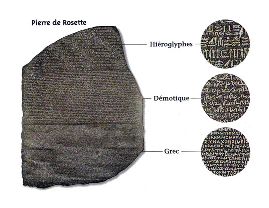
\includegraphics[width=6cm]{rosette}
      \end{minipage}
      \qquad
      \begin{minipage}{9.5cm}
         En 1821, Jean-François Champollion réussit à décrypter les caractères égyptiens. Comment a-t-il pu réussir cet exploit ? On pourra s'aider de l'image ci-contre. \\ [3mm]
         \pf \\ [3mm]
         \pf \\ [3mm]
         \pf
      \end{minipage}

      \bigskip
      
   \partie[la numération égyptienne]
      \begin{enumerate}
         \item Dans la numération égyptienne, voilà comment on écrit certains nombres indo-arabes : \smallskip
         \begin{center} 
            \begin{tabular}{|c|c|c|c|c|}
               \hline
               18 & 70 & 235 & 3\,018 & 1\,230\,012 \\
               \hline
               & & & & \\ [-3mm]
               \Large\textpmhg{\Hten\Hone\Hone\Hone\Hone\Hone\Hone\Hone\Hone}
               &
               \Large\textpmhg{\Hten\Hten\Hten\Hten\Hten\Hten\Hten}
               & 
               \Large\textpmhg{\Hhundred\Hhundred\Hten\Hten\Hten\Hone\Hone\Hone\Hone\Hone} & \Large\textpmhg{\Hthousand\Hthousand\Hthousand\Hten\Hone\Hone\Hone\Hone\Hone\Hone\Hone\Hone}
               &
               \Large\textpmhg{\Hmillion\HCthousand\HCthousand\HXthousand\HXthousand\HXthousand\Hten\Hone\Hone} \\
               \hline
            \end{tabular}
         \end{center} \medskip
      À la manière de Champollion, retrouver la valeur de ces symboles égyptiens. \smallskip
      \begin{center}
         \begin{tabular}{|C{1.8}|C{1.8}|C{1.8}|C{1.8}|C{1.8}|C{1.8}|C{1.8}|}
            \hline
            & & & & & & \\ [-3mm]
            \Large\textpmhg{\Hone}
            &
            \Large\textpmhg{\Hten}
            &
            \Large\textpmhg{\Hhundred}
            &
            \Large\textpmhg{\Hthousand}
            &
            \Large\textpmhg{\HXthousand}
            &
            \Large\textpmhg{\HCthousand}
            &
            \Large\textpmhg{\Hmillion} \\
            \hline
            & & & & & & \\ [3mm]
           \hline
         \end{tabular}
      \end{center}
 
      \bigskip
   
      \item Écrire les nombres égyptiens suivants en nombres indo-arabes : \\ [2mm]
      {\Large\textpmhg{\HXthousand\Hthousand\Hthousand\Hten\Hten\Hten\Hten\Hten\Hten}} : \pf \\ [3mm]
      {\Large\textpmhg{\HCthousand\HXthousand\HXthousand\HXthousand\Hthousand\Hthousand\Hthousand\Hhundred\Hhundred\Hhundred\Hten\Hten\Hten\Hten\Hone\Hone\Hone\Hone\Hone\Hone\Hone\Hone}} : \pf \\  [3mm]
      {\Large\textpmhg{\Hmillion\Hmillion\Hmillion\HCthousand\Hone\Hone}} : \pf \\
      \item Écrire les nombres indo-arabes suivants en nombres égyptiens : \\ [4mm]
      8\,032 : \pf \\ [5mm]
      3\,000\,100 :  \pf \\
      \item Quel nombre présent dans notre numération écrite n'existe pas dans la numération égyptienne ? Pourquoi ? \\ [3mm]
      \pf
      \end{enumerate}


\themaG
\graphicspath{{../Ch1_Premiers_elements_de_geometrie/Images/}}

\chapter{Du point à la droite}
\label{C02}

%%%%%%%%%%%%%%%%%%%%%%%%%%%%%%%%%%%%%%%%%%
\begin{prerequis}[Connaissances et compétences abordées]
   \begin{itemize}
      \item Alignement, appartenance.
      \item Segment de droite.
      \item Vocabulaire associé au milieu et à ses propriétés.
   \end{itemize}
\end{prerequis}

\vfill

\begin{debat}[Débat : les définition d'Euclide]
   La mathématicien grec {\it Euclide}, considéré comme le père de la géométrie, définit les objets géométriques au III\up{e} siècle av. J.-C. Son 1\up{er} livre comprend notamment les définitions suivantes :
   \begin{itemize}
      \item le {\bf point} est ce dont la partie est nulle ;
      \item une {\bf ligne} est une longueur sans largeur ;
      \item la {\bf ligne droite} est celle qui est également placée entre ses points.
   \end{itemize}
   \begin{pspicture}(-4,-0.25)(9,2.75)
      \psset{linecolor=B1}
      \psdot(0,1)
      \psbezier(2,0)(3,2)(4,0.5)(5,2)
      \psline(6,0)(9,2)
   \end{pspicture}
   \bigskip
   \begin{cadre}[B2][F4]
      \begin{center}
         Vidéo : \href{https://www.youtube.com/watch?v=enZpq8jvFEs}{\bf L'axiomatique. Les éléments d'Euclide}, chaîne YouTube de {\it Monsieur Phi}, de 2 min 30 s à 8 min.
      \end{center}
   \end{cadre}
\end{debat}

\vfill

\textcolor{PartieGeometrie}{\large\sffamily\bfseries Cahier de compétences} : $\varnothing$


%%%%%%%%%%%%%%%%%%%%%%%%%%%%%%%%%%%%
%%%%%%%%%%%%%%%%%%%%%%%%%%%%%%%%%%%%%
\activites

\begin{activite}[Faisceaux de traits]
   {\bf Objectifs :} employer des relations d'incidence comme l'appartenance d'un point
à un ou deux segments ou droites, intersection, alignement ; mise en place d'une chronologie de tracé. 
   \begin{QCM}
      \partie[première construction]
         {\psset{unit=0.7}
         \begin{pspicture}(-5,-1)(15,11)
            \pstGeonode[PointName=none,linewidth=1mm,PointSymbol=+](2,9){Z}(3.5,3){Y}(6,3.5){C}(8,6){D}(4,1){E}(5.42,4.27){F}(11,4.5){G}
            \pstLineAB[nodesepA=-4,nodesepB=-5]{C}{D}
            \pstLineAB[nodesepA=-1,nodesepB=-3]{Z}{Y}
            \pstLineAB[nodesepA=-4,nodesepB=-7]{Y}{D}
            \pstLineAB[nodesepA=-4,nodesepB=-8]{Y}{C}
            \pstLineAB[nodesepA=-1,nodesepB=-4]{Z}{C}
            \pstLineAB[nodesepA=-1,nodesepB=-7]{Z}{D}
         \end{pspicture}} \\
         Reproduire la figure ci-dessus en s'aidant des points d'intersection déjà placés. \\
         \begin{pspicture}(-4,0)(15,10)
            \pstGeonode[PointName=none,linewidth=1mm,PointSymbol=+](2,9){Z}(3.5,3){Y}(6,3.5){C}(8,6){D}
         \end{pspicture}
   \end{QCM}

   \begin{QCM}
      \partie[seconde construction]
       Reproduire la figure projetée au tableau en s'aidant des points d'intersection déjà placés. \\
         \begin{pspicture}(0.5,0)(15,19)
            \pstGeonode[PointName=none,linewidth=1mm,PointSymbol=+](9.5,5){Z}(10,6.5){Y}(10.5,13){C}(12.5,14){D}(15.5,2.5){E}
         \end{pspicture}
   \end{QCM}

\pagebreak

   Figure à projeter : \\
   \begin{pspicture}(0,0)(16,19) %PointName=none,
      \pstGeonode[linewidth=1mm,PointSymbol=+,PointName=none](9.5,5){A}(10,6.5){B}(10.5,13){C}(12.5,14){D}(15.5,2.5){E}
      \pstInterLL[linewidth=1mm,PointSymbol=+,PointName=none]{A}{E}{C}{D}{F}
      \pstInterLL[linewidth=1mm,PointSymbol=+,PointName=none]{B}{E}{C}{D}{G}
      \pstInterLL[linewidth=1mm,PointSymbol=+,PointName=none]{A}{G}{B}{F}{H}
      \pstInterLL[linewidth=1mm,PointSymbol=+,PointName=none]{B}{D}{C}{E}{I}
      \pstInterLL[linewidth=1mm,PointSymbol=+,PointName=none]{H}{D}{B}{G}{J}
      \pstInterLL[linewidth=1mm,PointSymbol=+,PointName=none]{B}{C}{G}{I}{K}
      \pstInterLL[linewidth=1mm,PointSymbol=+,PointName=none]{E}{C}{D}{H}{L}
      \pstLineAB[nodesepA=-10,nodesepB=-2]{A}{E}
      \pstLineAB[nodesepA=-10,nodesepB=-2]{B}{E}
      \pstLineAB[nodesepA=-3,nodesepB=-2]{A}{D}
      \pstLineAB[nodesepA=-12,nodesepB=-2]{C}{D}
      \pstLineAB[nodesepA=-3,nodesepB=-2]{C}{E}
      \pstLineAB{A}{G}
      \pstLineAB{B}{F}
      \pstLineAB{B}{F}
      \pstLineAB{H}{D}
      \pstLineAB{G}{I}
   \end{pspicture}
\end{activite}

 
%%%%%%%%%%%%%%%%%%%%%%%%%%%%%%%%%
%%%%%%%%%%%%%%%%%%%%%%%%%%%%%%%%%
\cours 

\section{Droites, demi-droites, segments} %%%%%%%%%

\begin{definition}
   \begin{itemize}
      \item Une {\bf droite} est une ligne rectiligne infinie. On peut noter une droite de différentes façons : \\
      \begin{pspicture}(-0.5,-0.7)(13,1)
         \pstGeonode[PosAngle=-90,PointSymbol=+](0,0){A}(3,0.5){B}
         \pstLineAB[nodesep=-0.5,linecolor=A1]{A}{B}
         \pstLabelAB{A}{B}{\small droite $(AB)$}
         \psline[linecolor=A1](4,0.25)(8,0)
         \rput(7.25,-0.35){$(d)$}
         \rput{-4}(6,0.5){\small droite $(d)$}
         \psline[linecolor=A1](8.5,-0.25)(12.5,0.5)
         \rput(9,-0.15){+}
         \rput(9,-0.5){$T$}
         \rput(12,0.2){$u$}
         \rput{9}(10.5,0.5){\small droite $(Tu)$}
      \end{pspicture}
      \item Une {\bf demi-droite} est une portion de droite limitée d'un seul côté par un point appelé origine. La demi-droite d'origine $A$ passant par $B$ se note $[AB)$. \\
      \begin{pspicture}(-5,-0.2)(5,1)
         \pstGeonode[PosAngle=180,PointSymbol=+](0,0){A}
         \pstGeonode[PosAngle=-90,PointSymbol=+](4,0.5){B}
         \pstLineAB[nodesepB=-1,linecolor=A1]{A}{B}
         \pstLabelAB{A}{B}{\small demi-droite $[AB)$}
      \end{pspicture}
      \item Un \textbf{segment} est une portion de droite limitée par deux points appelés extrémités. Le segment d'extrémités $A$ et $B$ se note $[AB]$ ou $[BA]$. \\
      \begin{pspicture}(-5,0.4)(5,1.2)
         \pstGeonode[PosAngle={180,-90},PointSymbol=+](0,0.2){A}(4,0.7){B}
         \pstLineAB[linecolor=A1]{A}{B}
         \pstLabelAB{A}{B}{\small segment $[AB]$}
      \end{pspicture}
   \end{itemize}
\end{definition}

\begin{exemple*1}
   \begin{minipage}{5cm}
      \begin{pspicture}(-1,-0.25)(4,1.8)
         \pstGeonode[PosAngle=-90,PointSymbol=+](0,0){A}(3,0){B}(2,1.25){C}
         \pstLineAB[nodesep=-0.5]{A}{B}
         \pstLineAB[nodesepB=-0.75]{A}{C}
         \pstLineAB{C}{B}
      \end{pspicture}
   \end{minipage}
   \begin{minipage}{6.5cm}
   \begin{itemize}
      \item $(AB)$ est une droite ;
      \item $[AC)$ est la demi-droite d'origine $A$ passant par $C$ ;
      \item $[CB]$ est le segment d'extrémités $C$ et $B$.
   \end{itemize}
   \end{minipage}
\end{exemple*1}


\section{Points particuliers} %%%%%%%%%

\begin{definition}
   Trois points sont {\bf alignés} s'ils appartiennent à une même droite.
   \begin{center}
   \begin{pspicture}(-2,-0.3)(11,-0.1)
      \pstGeonode[PosAngle=-90,PointSymbol=+](0,0){A}(4,0){B}(1.5,0){C}
      \pstLineAB[nodesep=-1]{A}{B}
      \rput(8,0){\small les points $A, B$ et $C$ sont alignés.}
   \end{pspicture}
   \end{center}
\end{definition}

\begin{notation}
   le symbole $\in$ signifie \og {\bf appartient} à \fg{} et $\not\in$ signifie \og n'appartient pas à \fg.
\end{notation}

\begin{exemple*1}
   On a par exemple $C\in(AB)$ et $B\in(AC)$ mais $A\notin[CB)$ et $B\notin[AC]$.
\end{exemple*1}

\begin{definition}
   Le {\bf milieu} $I$ du segment $[AB]$ est le point de ce segment qui est équidistant de $A$ et de $B$.
\end{definition}

\begin{remarque}
   la longueur d'un segment $[AB]$ se note $AB$, et pour indiquer que l'on a des mesures égales, c'est à dire $AI =IB$, on effectue un codage de la figure. \\
   Exemples de codes que l'on peut utiliser : \textcolor{B1}{\textsf x, +, o, /\!\!/} \dots
\end{remarque}

\begin{exemple*1}
   \begin{pspicture}(-1,1.5)(5,2) 
      \psline[linecolor=A1]{|-|}(0,1.5)(5,1.5)
      \psline[linecolor=B1](2.5,1.4)(2.5,1.6)
      \rput(0,1.9){$F$}
      \rput(2.5,1.9){$I$}
      \rput(5,1.9){$L$}
      \rput(1.25,1.5){\textcolor{B1}{\Large$\times$}}
      \rput(3.75,1.5){\textcolor{B1}{\Large$\times$}}
   \end{pspicture}
\end{exemple*1}

\medskip

\begin{definition}
   Deux droites sont {\bf sécantes} lorsqu'elles se coupent en un point appelé {\bf point d'intersection}.
\end{definition}


%%%%%%%%%%%%%%%%%%%%%%%%%%%%%%%%%%%%%%%%%%
\exercicesbase

\begin{colonne*exercice}

\serie{Droites, demi-droites, segments} %%%%%%%%%%%%%%%%%%%%%
 
\begin{exercice} %1
   Repasser en rouge la partie de la droite correspondant aux écritures mathématiques.
   \begin{enumerate}
      \item \begin{pspicture}(0,-0.1)(7,0.4)
                  \small
                  \psline(0,0)(6,0)
                  \pstGeonode[PointSymbol=+,PosAngle=-90](1,0){A}(2,0){B}(3,0){C}(4,0){D}(5,0){E}
                  \rput(7,0){$[AC)$}
               \end{pspicture}               
      \item \begin{pspicture}(0,-0.1)(7,0.7)
                  \small
                  \psline(0,0)(6,0)
                  \pstGeonode[PointSymbol=+,PosAngle=-90](1,0){D}(2.3,0){R}(3.1,0){O}(4.5,0){I}
                  \rput(5.7,-0.2){t}
                  \rput(7,0){$[IR]$}
               \end{pspicture}
      \item \begin{pspicture}(0,-0.1)(7,0.7)
                  \small
                  \psline(0,0)(6,0)
                  \pstGeonode[PointSymbol=+,PosAngle=-90](1.2,0){A}(2.2,0){U}(3.2,0){C}(4.2,0){H}(5.2,0){E}
                  \rput(0.2,-0.2){$g$}
                  \rput(7,0){$(gH]$}
               \end{pspicture} \\
   \end{enumerate}
\end{exercice}
 
\bigskip
 
\begin{exercice} %2
   Nommer la partie de la droite qui a été repassée en gras de deux manières différentes.
   \begin{enumerate}
      \item \begin{pspicture}(0,-0.1)(7,0.4)
                  \small
                  \psline(0,0)(6,0)
                  \pstGeonode[PointSymbol=+,PosAngle=-90](1,0){A}(2,0){B}(3,0){C}(4,0){D}(5,0){E}
                  \pstLineAB[linewidth=0.5mm]{C}{B}
               \end{pspicture}               
      \item \begin{pspicture}(0,-0.1)(7,0.7)
                  \small
                  \psline(0,0)(6,0)
                  \pstGeonode[PointSymbol=+,PosAngle=-90](1,0){D}(2.3,0){R}(3.1,0){O}(4.5,0){I}
                  \rput(5.7,-0.2){t}
                  \psline[linewidth=0.5mm](3.1,0)(6,0)
               \end{pspicture}
      \item \begin{pspicture}(0,-0.1)(7,0.7)
                  \small
                  \psline(0,0)(6,0)
                  \pstGeonode[PointSymbol=+,PosAngle=-90](1.2,0){A}(2.2,0){U}(3.2,0){C}(4.2,0){H}(5.2,0){E}
                  \rput(0.2,-0.2){$g$}
                  \psline[linewidth=0.5mm](0,0)(2.2,0)
               \end{pspicture} \\ [-1mm]
   \end{enumerate}
\end{exercice}

\bigskip

\begin{exercice} %3
   On considère la droite suivante : \\
   \begin{pspicture}(-1,-0.4)(7,0.4)
      \small
      \psline(0,0)(6,0)
      \pstGeonode[PointSymbol=+,PosAngle=-90](1,0){A}(2.25,0){B}(3.5,0){C}(5,0){D}
   \end{pspicture}           
   \begin{enumerate}
      \item Écrire tous les noms possibles pour cette droite.
      \item Combien y aurait-il de noms en plus si on avait placé cinq points sur la droite ?
      \item Combien faut-il de points pour que la droite ait six noms possibles ?
   \end{enumerate}
\end{exercice}

\bigskip

\serie{Points particuliers} %%%%%%%%%%%%%%%%%%%%%

\begin{exercice} %4
   Compléter les phrases à l'aide de la figure. \\
   {\psset{yunit=0.6}
   \small
   \begin{pspicture}(-0.3,-0.3)(8,5.3)
      \pstGeonode[PointSymbol=none,PosAngle={90,110,90,100,120,90}](1,4){A}(3.5,4){B}(7,4){C}(3,2.8){D}(2.5,1.3){E}(4,2.2){F}
      \pstLineAB[nodesepA=-1,nodesepB=-1]{A}{C}
      \pstLineAB[nodesepA=-0.8,nodesepB=-1.3]{B}{E}
      \pstLineAB[nodesepA=-1,nodesepB=-3]{A}{F}
      \pstLineAB[nodesepA=-1,nodesepB=-2]{C}{E}
      \rput(6.5,1.1){$(d_1)$}
      \rput(0.4,3.6){$(d_2)$}
      \rput(1,0.8){$(d_3)$}
      \rput(2.6,0.3){$(d_4)$}
   \end{pspicture}}
   \begin{enumerate}
      \item Les droites $(d_1)$ et $(d_2)$ se coupent en \pfb
      \item Le point d'intersection de $(d_1)$ et $(d_3)$ est \pfb
      \item $C$ est le point d'intersection de \pfb et \pfb
      \item Le point $B$ est à l'intersection de \pfb et \pfb
   \end{enumerate}
\end{exercice}

\bigskip

\begin{exercice} %5
   Compléter avec $\in$ ou $\notin$. \\
   \begin{pspicture}(-0.3,-0.1)(7,0.6)
      \small
      \psline(0,0)(7.5,0)
      \pstGeonode[PointSymbol=+,PosAngle=90](1,0){O}(3,0){U}(6,0){F}
   \end{pspicture}  
   \begin{colenumerate}{3}
      \item $O \pfb [UF]$
      \item $O \pfb [UF)$
      \item $O \pfb (UF)$
      \item $U \pfb [FO)$
      \item $U \pfb [OF)$
      \item $F \pfb (OU)$
   \end{colenumerate}
\end{exercice}

\bigskip

\begin{exercice} %6
   Compléter avec $\in$ ou $\notin$. \\
   {\psset{yunit=0.6}
   \begin{pspicture}(-0.5,0.6)(8,5.2)
      \pstGeonode[PointSymbol=+,PosAngle={90,110,90,100,120,90}](1,4){Q}(5,4){X}(7,4){M}(3.63,2.52){O}(2.5,1.3){L}(6,1.2){Z}(1,2){V}
      \pstLineAB[nodesepA=-1,nodesepB=-0.5]{Q}{M}
      \pstLineAB[nodesepA=-0.8,nodesepB=-1]{Q}{Z}
      \pstLineAB[nodesepB=-1]{L}{X}
   \end{pspicture}}
   \begin{colenumerate}{3}
      \item $X \pfb (QM)$
      \item $X \pfb [QM]$
      \item $Q \pfb [XM]$
      \item $X \pfb [QM)$
      \item $Q \pfb (OZ)$
      \item $O \pfb [LX]$
      \item $L \pfb [XO)$
      \item $V \pfb (OM)$
      \item $L \pfb [OX)$
   \end{colenumerate}
\end{exercice}

\bigskip

\begin{exercice} %7
   Vrai (V) ou faux (F) ?
   \begin{enumerate}
      \item Si $C \in (AB)$ alors $A \in (BC)$.
      \item Si $E \in [DF]$ alors $D \in [EF]$.
      \item Si $C \in [AB)$ mais $C \notin [AB]$ alors $A \in [CB)$.
      \item Si $C \in [BA)$ mais $C \notin [AB]$ alors $B \in [AC)$.
   \end{enumerate}
\end{exercice}

\bigskip

\begin{exercice} %8
   En s'aidant des points déjà marqués, placer les points $H, I, L$ et $M$. \\
   {\psset{yunit=0.5}
   \begin{pspicture}(-0.5,0)(8,5.5)
      \pstGeonode[PointSymbol=+,PosAngle=90](1.5,4){A}(3.5,2){B}(5.5,4){C}(7,1){D}(0.5,0.5){E}
   \end{pspicture}}
   \begin{colenumerate}{2}
      \item $H \in [AB)$ et $H \in [ED]$
      \item $I \in [CB)$ et $I \in [ED]$
      \item $L \in [BD]$ et $L \in [CH]$
      \item $M \in [AI)$ et $M \in [DH)$
   \end{colenumerate}
\end{exercice}

\bigskip

\begin{exercice}
   Construire le milieu de chaque segment sans utiliser d'instrument de géométrie. Coder la figure.
   \begin{center}
   \psset{xunit=0.5,yunit=0.4}
      \begin{pspicture}(0,0)(13,9)
         \psgrid[gridlabels=0,subgriddiv=0,gridcolor=lightgray](0,0)(13,9)
         \pstGeonode[PointSymbol=+,dotangle=45,PosAngle=-80](1,2){A}(7,2){B}(1,4){C}(2,8){D}(8,8){E}(12,2){F}(4,5){G}(8,4){H}
         \pstLineAB{A}{B}
         \pstLineAB{C}{D}
         \pstLineAB{E}{F}
         \pstLineAB{G}{H}
      \end{pspicture}
   \end{center}
\end{exercice}

\flushright{\it\footnotesize Source : Les cahiers Sesamath 6\up{e}. Magnard-Sésamath 2017.}
\end{colonne*exercice}


%%%%%%%%%%%%%%%%%%%%%%%%%%%%%%%%%%%%%%%%%%
\Recreation

\enigme[La pipopipette]
   \partie[présentation du jeu]
      La pipopipette ou \og jeu des petits carrés \fg{} est un jeu se pratiquant à deux joueurs en tour par tour dont l'idée serait attribuée à des élèves de l'École polytechnique à la fin du {\small XIX}\up{e} siècle : pipo désignait à l'époque cette école en argot. \\
      {\bf But du jeu :} former des carrés. Le gagnant est celui qui a fermé le plus de carrés. \\
      {\bf Règles du jeu :}
         \begin{itemize}
            \item À chaque tour, chaque joueur trace un petit segment suivant le quadrillage de la feuille.
            \item Chaque fois qu'un joueur peut fermer un carré, il marque le carré de son signe rejoue.
            \item Quand la grille est remplie, on compte le nombre de carrés fermés pour chaque joueur.
         \medskip
         \end{itemize}
      {\bf Exemple avec un terrain de 2 $\times$ 2:}
         \begin{center}
         {\psset{unit=0.7}
            \begin{tabular}{*{6}{C{2.4}}}
               \begin{pspicture}(0,0)(2,1.8)
                  \psgrid[subgriddiv=0,gridlabels=0,gridcolor=lightgray](0,0)(2,2)
                  \psset{linewidth=0.5mm}
                  \psline[linecolor=A1](0,2)(1,2)
               \end{pspicture}
               &
               \begin{pspicture}(0,0)(2,1.8)
                  \psgrid[subgriddiv=0,gridlabels=0,gridcolor=lightgray](0,0)(2,2)
                  \psset{linewidth=0.5mm,linecolor=A1}
                  \psline(0,2)(1,2)
                  \psset{linecolor=B1}
                  \psline(1,0)(2,0)
               \end{pspicture}
               &
               \begin{pspicture}(0,0)(2,1.8)
                  \psgrid[subgriddiv=0,gridlabels=0,gridcolor=lightgray](0,0)(2,2)
                  \psset{linewidth=0.5mm,linecolor=A1}
                  \psline(0,2)(2,2)
                  \psset{linecolor=B1}
                  \psline(1,0)(2,0)
               \end{pspicture}
               &
               \begin{pspicture}(0,0)(2,1.8)
                  \psgrid[subgriddiv=0,gridlabels=0,gridcolor=lightgray](0,0)(2,2)
                  \psset{linewidth=0.5mm,linecolor=A1}
                  \psline(0,2)(2,2)
                  \psset{linecolor=B1}
                  \psline(0,0)(2,0)
               \end{pspicture}
               &
               \begin{pspicture}(0,0)(2,1.8)
                  \psgrid[subgriddiv=0,gridlabels=0,gridcolor=lightgray](0,0)(2,2)
                  \psset{linewidth=0.5mm,linecolor=A1}
                  \psline(0,1)(0,2)(2,2)
                  \psset{linecolor=B1}
                  \psline(0,0)(2,0)
               \end{pspicture}
               &
               \begin{pspicture}(0,0)(2,1.8)
                  \psgrid[subgriddiv=0,gridlabels=0,gridcolor=lightgray](0,0)(2,2)
                  \psset{linewidth=0.5mm,linecolor=A1}
                  \psline(0,1)(0,2)(2,2)
                  \psset{linecolor=B1}
                  \psline(0,0)(2,0)(2,1)
               \end{pspicture} \\
               \textcolor{A1}{joueur 1} & \textcolor{B1}{joueur 2} & \textcolor{A1}{joueur 1} & \textcolor{B1}{joueur 2} & \textcolor{A1}{joueur 1} & \textcolor{B1}{joueur 2} \\ [5mm]
               \begin{pspicture}(0,0)(2,2)
                  \psgrid[subgriddiv=0,gridlabels=0,gridcolor=lightgray](0,0)(2,2)
                  \psset{linewidth=0.5mm,linecolor=A1}
                  \psline(1,1)(0,1)(0,2)(2,2)
                  \psset{linecolor=B1}
                  \psline(0,0)(2,0)(2,1)
               \end{pspicture}
               &
               \begin{pspicture}(0,0)(2,2)
                  \psgrid[subgriddiv=0,gridlabels=0,gridcolor=lightgray](0,0)(2,2)
                  \psset{linewidth=0.5mm,linecolor=A1}
                  \psline(1,1)(0,1)(0,2)(2,2)
                  \psset{linecolor=B1}
                  \psline(0,0)(2,0)(2,1)
                  \psline(1,1)(1,2)
                  \psdot[dotstyle=+](0.5,1.5)
               \end{pspicture}
               &
               \begin{pspicture}(0,0)(2,2)
                  \psgrid[subgriddiv=0,gridlabels=0,gridcolor=lightgray](0,0)(2,2)
                  \psset{linewidth=0.5mm,linecolor=A1}
                  \psline(1,1)(0,1)(0,2)(2,2)
                  \psset{linecolor=B1}
                  \psline(0,1)(0,0)(2,0)(2,1)
                  \psline(1,1)(1,2)
                  \psdot[dotstyle=+](0.5,1.5)
               \end{pspicture}
               &
               \begin{pspicture}(0,0)(2,2)
                  \psgrid[subgriddiv=0,gridlabels=0,gridcolor=lightgray](0,0)(2,2)
                  \psset{linewidth=0.5mm,linecolor=A1}
                  \psline(1,0)(1,1)(0,1)(0,2)(2,2)
                  \psdot[dotstyle=*](0.5,0.5)
                  \psset{linecolor=B1}
                  \psline(0,1)(0,0)(2,0)(2,1)
                  \psline(1,1)(1,2)
                  \psdot[dotstyle=+](0.5,1.5)
               \end{pspicture}
               &
               \begin{pspicture}(0,0)(2,2)
                  \psgrid[subgriddiv=0,gridlabels=0,gridcolor=lightgray](0,0)(2,2)
                  \psset{linewidth=0.5mm,linecolor=A1}
                  \psline(1,0)(1,1)(0,1)(0,2)(2,2)
                  \psline(1,1)(2,1)
                  \psdots[dotstyle=*](0.5,0.5)(1.5,0.5)
                  \psset{linecolor=B1}
                  \psline(0,1)(0,0)(2,0)(2,1)
                  \psline(1,1)(1,2)
                  \psdot[dotstyle=+](0.5,1.5)
               \end{pspicture}
               &
                \begin{pspicture}(0,0)(2,2)
                 \psgrid[subgriddiv=0,gridlabels=0,gridcolor=lightgray](0,0)(2,2)
                  \psset{linewidth=0.5mm,linecolor=A1}
                  \psline(1,0)(1,1)(0,1)(0,2)(2,2)
                  \psline(1,1)(2,1)(2,2)
                  \psdots[dotstyle=*](0.5,0.5)(1.5,0.5)(1.5,1.5)
                  \psset{linecolor=B1}
                  \psline(0,1)(0,0)(2,0)(2,1)
                  \psline(1,1)(1,2)
                  \psdot[dotstyle=+](0.5,1.5)
               \end{pspicture}
               \\
               \textcolor{A1}{joueur 1} & \textcolor{B1}{joueur 2} & \textcolor{B1}{joueur 2} & \textcolor{A1}{joueur 1} & \textcolor{A1}{joueur 1} & \textcolor{A1}{joueur 1} \\
            \end{tabular}}
         \end{center}
      Le \textcolor{A1}{joueur 1} a pris possession de trois carrés alors que le \textcolor{B1}{joueur 2} en a un seul, c'est donc le \textcolor{A1}{joueur 1} qui gagne. \\

   \partie[à vous de jouer !!!]
      En binôme, compléter  ces grilles.
      \begin{center}
         \begin{tabular}{C{2}C{3.1}C{4.2}C{5}}
            \begin{pspicture}(0,0)(2,2)
               \psgrid[subgriddiv=0,gridlabels=0,gridcolor=lightgray](0,0)(2,2)
            \end{pspicture}
            &
            \begin{pspicture}(0,0)(3,3)
               \psgrid[subgriddiv=0,gridlabels=0,gridcolor=lightgray](0,0)(3,3)
            \end{pspicture}
            &
            \begin{pspicture}(0,0)(4,4)
               \psgrid[subgriddiv=0,gridlabels=0,gridcolor=lightgray](0,0)(4,4)
            \end{pspicture}
           &
           \begin{pspicture}(0,0)(5,4.5)
               \psgrid[subgriddiv=0,gridlabels=0,gridcolor=lightgray](0,0)(5,5)
            \end{pspicture} \\ [5mm]
         \end{tabular} \\
         \begin{tabular}{C{6.2}C{9}}
            \begin{pspicture}(0,0)(6,3)
               \psgrid[subgriddiv=0,gridlabels=0,gridcolor=lightgray](0,0)(6,3)
            \end{pspicture}
            &
            \begin{pspicture}(0,0)(9,3.5)
               \psgrid[subgriddiv=0,gridlabels=0,gridcolor=lightgray](0,0)(9,4)
            \end{pspicture} \\
         \end{tabular}
      \end{center}


\themaN
\graphicspath{{../Ch2_Nombres_entiers_et_decimaux/Images/}}

\chapter{Fractions et\\nombres décimaux}
\label{C03}

%%%%%%%%%%%%%%%%%%%%%%%%%%%%%%%%%%%%%
\begin{prerequis}[Connaissances et compétences abordées]
   \begin{itemize}
      \item Connaître les unités de la numération décimale (unités simples, dixièmes, centièmes, millièmes) et les relations qui les lient.
      \item Connaître la valeur des chiffres en fonction de leur rang.
      \item Connaître et utiliser diverses désignations orales et écrites d’un nombre décimal (fractions décimales, écritures à virgule, décompositions additives et multiplicatives).
   \end{itemize}
\end{prerequis}

\vfill

\begin{debat}[Débat : un peu d'histoire]
   Le système de numération que nous employons actuellement et qui nous semble si naturel est le fruit d'une longue évolution des concepts mathématiques. En effet, un nombre est une entité abstraite qui peut surprendre : on a déjà vu {\bf un} élève, {\bf un} animal donné, on sait ce qu'est {\bf un} jour, mais qu'est-ce que {\bf un} ? C'est une entité qui, prise seule, n'a pas vraiment de sens. De nombreuses civilisations ont imaginé des systèmes de numération plus ou moins compliqués, plus ou moins pratiques : des systèmes utilisant des bases différentes, des systèmes utilisant le principe additif\dots{} jusqu'à notre système de numération positionnel de base dix maintenant utilisé de manière universelle. \\
   \begin{center}
      \textcolor{B1}{{\huge 19\textcircled{\Large 0}1\textcircled{\Large 1}7\textcircled{\Large2}8\textcircled{\Large 3}} \\ [3mm]
      \it Notation décimale de Simon Stevin \\
      représentant le nombre 19,178.}
   \end{center}
   \bigskip
   \begin{cadre}[B2][F4]
      \begin{center}
         Vidéo : \href{https://www.youtube.com/watch?v=bkGMa1EJkSA}{\bf Histoire de la virgule}, chaîne Youtube de {\it Maths 28}.
      \end{center}
   \end{cadre}
\end{debat}

\vfill

\textcolor{PartieGeometrie}{\large\sffamily\bfseries Cahier de compétences} : chapitre 1 pages 8 et 9 exercices 2 à 16. 


%%%%%%%%%%%%%%%%%%%%%%%%%%%%%%%%%%
%%%%%%%%%%%%%%%%%%%%%%%%%%%%%%%%%%
\activites

\begin{activite}[La droite graduée]
   {\bf Objectifs :} comprendre et utiliser le principe de construction d'une graduation régulière en dixièmes et en centièmes ; savoir situer des nombres décimaux sous différents écritures. \\
\begin{QCM}
      \partie[construction d'une droite graduée]
         \begin{enumerate}
            \item Sur la bande de papier fournie, tracer au stylo une droite la plus longue possible. \\
            \item Placer à gauche sur cette droite le repère de l'origine puis inscrire la valeur 0 en dessous. \\
            \item Combien faut-il aligner de petites bandes de valeur \og $\dfrac1{10}$ \fg{} pour obtenir 1 ? Justifier. \\ [3mm]
            \pf \\
            \begin{center}
               \begin{pspicture}(0,-0.25)(5,1.75)
                  \multido{\n=0+0.5}{11}{\psline(\n,0)(\n,0.5)}
                  \psframe[fillstyle=solid,fillcolor=J1](0,0.5)(5,1.5)
                  \psline(0,0)(5,0)
                  \rput(2.5,1){\white $\dfrac1{10}$}
               \end{pspicture}
            \end{center}
            \item Grâce cette petite bande de couleur, placer le nombre 1. \\
            \item Placer ensuite les nombres 2 et 3 de la même manière, toujours en dessous de la droite. \medskip
         \end{enumerate}
         
      \partie[placer des nombres décimaux sur la droite graduée]
         \begin{enumerate}
            \setcounter{enumi}{5}
            \item Sur la droite graduée, placer au crayon à papier et au-dessus les nombres suivants :
               $$\dfrac{8}{10} \hspace{2cm} \dfrac{23}{10} \hspace{2cm} 2+\dfrac{1}{10}$$
            \item Sur la droite graduée, placer au crayon à papier et au-dessus les nombres suivants :
               $$\text{cinq dixièmes} \hspace{2cm} \text{douze dixièmes}$$
            \item Sur la droite graduée, placer au crayon à papier et au-dessus les nombres suivants :
               $$0,3 \hspace{2cm} 1,7$$
            \item Trouver un moyen pour placer $\dfrac{143}{100}$ sur la droite graduée. \\
            \item \, Placer au crayon les nombres suivants :
               $$\dfrac{255}{100} \hspace{2cm} \text{cent-six centièmes} \hspace{2cm} 1+\dfrac{9}{10}+\dfrac{8}{100} \hspace{2cm} 0,23$$
         \end{enumerate}
      \end{QCM}
   \vfill\hfill{\it\footnotesize Source : Apprentissages numériques et résolution de problèmes au CM2, Ermel, Hatier 2001}.
\end{activite}


%%%%%%%%%%%%%%%%%%%%%%%%%%%%%%%%%%%%%
\cours 

\section{Des fractions décimales aux nombres décimaux}

\begin{definition}
   Une {\bf fraction décimale} est une fraction dont le dénominateur est  1, 10, 100, 1\,000 \dots \\
   Un {\bf nombre décimal} est un nombre qui peut s'écrire sous forme d'une fraction décimale.
\end{definition}

\begin{exemple*1}
   \begin{itemize}
      \item Les fractions décimales les plus \og simples \fg{} sont $\dfrac{1}{10} \; ; \; \dfrac{1}{100} \; ; \;\dfrac{1}{1\,000}, \; ; \;\dfrac{1}{10\,000}$ \dots{}
      \item  Mais $\dfrac{7}{10} \; ; \; \dfrac{32}{1\,000}  \; ; \; \dfrac{99\,999}{100\,000}$ sont également des fractions décimales.
      \item 1,8 est un nombre décimal car il peut s'écrire sous la forme $\dfrac{18}{10}$. \\ [-9mm]
   \end{itemize}
\end{exemple*1}

\begin{remarque}
   tout nombre entier est un nombre décimal \og caché \fg : par exemple $\dfrac{3}{1} =3$.
\end{remarque}

Un nombre a une seule valeur numérique mais a plusieurs écritures.
   
\begin{exemple*1}
   Voilà plusieurs écritures du nombre 16,82 : \par\medskip
    {\hautab{1.5}
    \begin{tabular}{cp{7cm}p{4cm}}
      16,82 & $=\dfrac{1\,682}{100}$ & fraction décimale \\
      & $=16+\dfrac{82}{100}$ & décompositions additives \\
      & $=(1\times10)+(6\times1)+\left(8\times\dfrac{1}{10}\right)+\left(2\times\dfrac{1}{100}\right)$ & \\
      & $= (1\times10)+(6\times1)+(8\times0,1)+(2\times0,01)$ & \\  
   \end{tabular}}
\end{exemple*1}


\section{Écrire des nombres décimaux} %%%%%%%%%%

\begin{propriete}
   On peut écrire un nombre décimal dans un tableau de numération comportant une partie entière identique aux nombres entiers à laquelle on ajoute une partie décimale :
   \begin{center}
      {\hautab{1.5}
      \begin{Ltableau}{0.9\linewidth}{16}{c}
         \hline
        \multicolumn{12}{|c@{\bf , }}{\bf partie entière} & \multicolumn{4}{c|}{\bf partie décimale} \\
         \hline
         \multicolumn{3}{|c|}{classe des} & \multicolumn{3}{c|}{classe des} & \multicolumn{3}{c|}{classe des} & \multicolumn{3}{c|}{classe des} & \multirow{3}*{\rotatebox{90}{dixièmes}} & \multirow{3}*{\rotatebox{90}{centièmes}} & \multirow{3}*{\rotatebox{90}{millièmes}} & \multirow{3}*{\rotatebox{90}{dix-millièmes}} \\
         \multicolumn{3}{|c|}{milliards} & \multicolumn{3}{c|}{millions} & \multicolumn{3}{c|}{milliers} & \multicolumn{3}{c|}{unités} & & & & \\
         c & d & u & c & d & u & c & d & u & c & d & u & & & & \\
         \hline
         & & 1 & 0 & 3 & 0 & 2 & 8 & 8 & 0 & 1 & 6 & 8 & 0 & 7 & \\
         \hline
      \end{Ltableau}}
   \end{center}  
\end{propriete}

\begin{exemple}
   Dans le nombre 1\,030\,288\,016,807 :
   \correction
   \textcolor{white}{.} \\[-29pt]
   \begin{itemize}
      \item le chiffre des dizaines de millions est 3 ;
      \item le chiffre des dixièmes est 8 ;
      \item le chiffre des centièmes est 0 ;
      \item le chiffre des millièmes est 7.
   \end{itemize}
\end{exemple}


%%%%%%%%%%%%%%%%%%%%%%%%%%%%%%%%%%%%%%%%%%
\exercicesbase

\begin{colonne*exercice}

\serie{Construction des nombres décimaux} %%%%%%%%%%%%%%%%%%%%

\begin{exercice}
   Associer chaque fraction décimale à son écriture décimale.
   \begin{center}
      \begin{tabular}{rp{1cm}l}
         $\dfrac{24}{100} \quad \bullet$ & & $\bullet \quad 204$ \\ [4mm]
         $\dfrac{2\,040}{10} \quad \bullet$ & & $\bullet \quad 2,4$ \\ [4mm]
         $\dfrac{204}{100} \quad \bullet$ & & $\bullet \quad 0,24$ \\ [4mm]
         $\dfrac{24}{10} \quad \bullet$ & & $\bullet \quad 2,04$ \\
      \end{tabular}
   \end{center}
\end{exercice}

\smallskip

\begin{exercice}
   Donner l'écriture décimale des nombres suivants :
   \begin{center}
      $\dfrac{45}{100} \; ; \; \dfrac{186}{10} \; ; \; \dfrac{5}{1\,000} \; ; \; \dfrac{6\,921}{100} \; ; \; \dfrac{850}{10} \; ; \; \dfrac{204}{1\,000}$
   \end{center}
\end{exercice}

\smallskip

\begin{exercice}
   Donner l'écriture en fraction décimale des nombres suivants :
   \begin{center}
      1,7 \; ; \; 25,04 \; ; \; 0,37 \; ; \; 4,005 \; ; \; 0,0592 \; ; \; 9,067
   \end{center}
\end{exercice}

\smallskip

\begin{exercice}
   Compléter le tableau suivant :
   \begin{center}
      {\hautab{1.8}
      \begin{ltableau}{0.97\linewidth}{4}
         \hline
         partie entière & partie décimale & fraction décimale & nombre décimal \\
         \hline
         51 &  2 & $\dfrac{512}{10}$ & $51,2$ \\
         \hline
         3 &  72 &  & \\
         \hline
         &  & & 0,81 \\
         \hline
         & & $\dfrac{330}{100}$ & \\
         \hline
         & & & 64,615 \\
         \hline
      \end{ltableau}}
   \end{center}
\end{exercice}

\smallskip

\begin{exercice}
   Associer chaque nombre de la première colonne à un nombre de la deuxième colonne.
   \begin{center}
      \begin{tabular}{rp{1cm}l}
         67 dixièmes \quad $\bullet$ & & $\bullet$ \quad 67 \\
         670 millièmes \quad $\bullet$ & & $\bullet $\quad 6\,700 \\
         670 dixièmes \quad $\bullet$ & & $\bullet$ \quad 0,67 \\
         67 millièmes \quad $\bullet$ & & $\bullet $\quad 0,006\,7 \\
         67 dix-millièmes \quad $\bullet$ & & $\bullet $\quad 0,067 \\
         67 centaines \quad $\bullet$ & & $\bullet $\quad 6,7 \\
      \end{tabular}
   \end{center}
\end{exercice}

\begin{exercice}
Dans le nombre 4 091,807 :
   \begin{enumerate}
      \item le chiffre des dixièmes est \pfb
      \item le chiffre des unités est \pfb
      \item le chiffre des millièmes est \pfb
      \item le chiffre des centaines est \pfb
      \item 409 est le nombre de \pfb
      \item 4 091 807 est le nombre de \pfb
      \item 40 est le nombre de \pfb
      \item 40 918 est le nombre de \pfb
   \end{enumerate}
\end{exercice}

\smallskip

\begin{exercice}
   Réécrire les nombres suivants en supprimant les zéros inutiles : \\
   5,00 \, ; \, 0204,02 \, ; \,0,230 \, ; \, 05\,020 \, ; \,1000,0800 \, ; \,00,010.
\end{exercice}

\smallskip

\serie{Composer/décomposer des nombres} %%%%%%%%%%%%%%%%%%%

\begin{exercice}
   Décomposer ainsi : $\dfrac{736}{100} =7+\dfrac{3}{10}+\dfrac{6}{100}$.
   \begin{center}
      $\dfrac{8\,725}{1\,000}$ \; ; \; $\dfrac{1\,253}{100}$ \; ; \; $\dfrac{32}{100}$ \; ; \; $\dfrac{908}{10}$
   \end{center}
\end{exercice}

\begin{exercice}
   Écrire sous forme d'une fraction décimale. \smallskip
   \begin{colenumerate}{2}
      \item $7+\dfrac{6}{10}$ \smallskip
      \item $45+\dfrac{8}{10}$ \smallskip
      \item $9+\dfrac{7}{1\,000}$ \smallskip
      \item $80+\dfrac{3}{10}+\dfrac{1}{100}$ \smallskip
      \item $3+\dfrac{2}{100}+\dfrac{5}{10}$ \smallskip
      \item $\dfrac{6}{10}+\dfrac{1}{1\,000}$ \smallskip
      \item $7+\dfrac{4}{10}+\dfrac{7}{100}+\dfrac{9}{1\,000}$ \smallskip
      \item $123+\dfrac{2}{1\,000}+\dfrac{4}{100}$
   \end{colenumerate}
\end{exercice}

\begin{exercice}
   Parmi ces écritures, quelles sont celles qui sont égales à 123,45 ? \smallskip
   \begin{colenumerate}{3}
      \item $12+\dfrac{345}{1\,000}$ \smallskip
      \item \small$123+\dfrac{4}{10}+\dfrac{5}{100}$ \smallskip
      \item $123+0,45$ \smallskip
      \item $\dfrac{12\,345}{10\,000}$ \smallskip
      \item $\dfrac{1\,234}{1\,000}+\dfrac{5}{100}$ \smallskip 
      \item $\dfrac{1\,234}{10}+5$ \smallskip
      \item $\dfrac{1\,234}{10}+\dfrac{5}{1\,000}$ \smallskip
      \item $1+\dfrac{2\,345}{100}$ \smallskip
      \item $123+\dfrac{45}{100}$
   \end{colenumerate}
\end{exercice}

\begin{exercice}
   Je suis un nombre qui peut s'écrire avec quatre chiffres et une virgule ; mon chiffre des unités est le double de mon chiffre des centièmes ; mon chiffre des dizaines est le triple de mon chiffre des dixièmes ; mon chiffre des centièmes est quatre ; lorsqu'on ajoute mes quatre chiffres, on obtient le nombre d'heures qu'il y a dans une journée. Qui suis-je ?
\end{exercice}

\end{colonne*exercice}

\begin{flushright}
   {\it\footnotesize Sources : Les cahiers Sesamath 6\up{e}. Magnard-Sésamath 2017 \& Delta Maths 6\up{e}. Magnard 2016.}
\end{flushright}


%%%%%%%%%%%%%%%%%%%%%%%%%%%%%%%%%%%%
%%%%%%%%%%%%%%%%%%%%%%%%%%%%%%%%%%%%%
\Recreation

\enigme[L'abaque romain\dots{} bis repetita]
      \partie[construction d'un l'abaque \og décimal \fg]
         À la manière de l'abaque romain construit dans le chapitre 1 (Nombres entiers), nous allons construire un abaque décimal \og moderne \fg. \\
         Reproduire cet abaque au verso de l'abaque romain toujours en mode paysage : sachant qu'il y a six colonnes, quelle peut être la largeur d'une colonne ? \pfb
         \begin{center}
            {\psset{unit=0.5}
            \begin{pspicture}(0,-0.5)(30,15)
               \multido{\i=0+5}{7}{\psline(\i,0)(\i,13)}
               \psset{linewidth=0.6mm}
               \psline(0,0)(0,14)(30,14)(30,0)
               \psline(15,0)(15,14)
               \psline(0,12)(30,12)
               \textcolor{B1}{\texttt{
               \rput(27.5,12.5){\large{millièmes}}
               \rput(22.5,12.5){\large{centièmes}}
               \rput(17.5,12.5){\large{dixièmes}}
               \rput(22.5,13.5){partie décimale}}}
               \textcolor{A1}{\texttt{
               \rput(12.5,12.5){\large\texttt{unités}}
               \rput(7.5,12.5){\large\texttt{dizaines}}
               \rput(2.5,12.5){\large\texttt{centaines}}
               \rput(7.5,13.5){partie entière}}}
            \end{pspicture}}
         \end{center}
         
      \partie[utilisation de l'abaque]
         \begin{enumerate}
            \item Rappeler les règles d'utilisation de l'abaque : qu'est-ce qui le différencie de l'abaque au recto ?
            \item Prendre un jeton et le placer dans l'une des colonnes de l'abaque. Quel nombre est représenté ? \\ [1mm]
               \pf \medskip
            \item Combien de nombres différents peut-on représenter avec un jeton ? Les lister en donnant la forme fractionnaire décimale et la forme décimale. \\ [2mm]
               \pf \\ [4mm]
               \pf \bigskip
            \item Combien de nombres différents peut-on représenter avec deux jetons ? En donner cinq sous forme fractionnaire et décimale. \\ [2mm]
               \pf \bigskip
            \item Représenter les nombres suivants :
               \begin{colitemize}{2}
                  \item 1,23
                  \item trente-six et deux dixièmes et trois millièmes
                  \item 0,317
                 \item cent-vingt-quatre centièmes                    
               \end{colitemize}
            \item Quels sont les nombres représentés sur l'abaque au tableau ? \\ [2mm]
               \pf
         \end{enumerate}


\themaG
\graphicspath{{../Ch7_Position_relative_de_deux_droites/Images/}}

\chapter{Position relative\\de deux droites}
\label{C04}

%%%%%%%%%%%%%%%%%%%%%%%%%%%%%%%%%%%%%%%%%%
\begin{prerequis}[Connaissances et compétences abordées]
   \begin{itemize}
      \item Perpendicularité, parallélisme.
   \end{itemize}
\end{prerequis}

\vfill

\begin{debat}[Débat : un peu de vocabulaire] 
   {\bf Perpendiculaire} : chez les Romains, {\it perpendiculum} désigne le fil à plomb ; en ancien français, un {\it perpendicle} est aussi un fil à plomb mais signifie également verticale et ce n'est  que dans la deuxième moitié du {\small XVI}\up{e} siècle que le mot {\it perpendiculaire} prend le sens que nous connaissons actuellement. \\
   {\bf Parallèle} : chez les Grecs, {\it parallelos} signifie \og placé en regard \fg{} et désigne aussi des cercles concentriques. Le mot est formé à partir de {\it para}, \og à côté \fg{} et de {\it allelon}, \og les uns et les autres \fg{}. Le mot parallèle est introduit au {\small XVI}\up{e} siècle dans le vocabulaire mathématique.
   {\centerline{\footnotesize\it Source : Les mots et les maths, Bertrand Hauchecorne, ellipses poche 2014.}}
   \begin{center}
      \begin{pspicture}(0,-0.5)(5,2.5)
         \psset{linecolor=B1,linewidth=1mm}
         \psline(0,0)(2,0)
         \psline(1,0)(1,2)
         \psline(3.5,0)(4.5,2)
         \psline(4,0)(5,2)
      \end{pspicture}
   \end{center}
   \begin{cadre}[B2][F4]
      \begin{center}
         Vidéo : \href{https://lesfondamentaux.reseau-canope.fr/video/reconnaitre-des-droites-perpendiculaires.html}{\bf Reconnaître des droites perpendiculaires}, et \href{https://lesfondamentaux.reseau-canope.fr/video/reconnaitre-des-droites-paralleles.html}{\bf Reconnaître des droites parallèles} du site {\it Canopé}, épisode de la série {\it Les fondamentaux}.
      \end{center}
   \end{cadre}
\end{debat}

\vfill

\textcolor{PartieGeometrie}{\large\sffamily\bfseries Cahier de compétences} : chapitre 7, exercices 1. 

%%%%%%%%%%%%%%%%%%%%%%%%%%%%%%%%%%%%
%%%%%%%%%%%%%%%%%%%%%%%%%%%%%%%%%%%%%
\activites

\begin{activite}[D'équerre ou pas d'équerre ?]
   {\bf Objectifs :} repérer des angles droits ; utiliser des instruments pour vérifier qu'un angle est droit ; coder une figure.
   \begin{QCM}
      \partie[construction d'un gabarit d'angle droit en papier]
         Pour vérifier qu'un angle est droit, on peut utiliser une équerre, mais il est facile de construire un gabarit d'angle droit avec un simple morceau de papier :
         \begin{center}
            \begin{pspicture}(0,0)(4,4.5)
               \psline(0,4)(0,1.5)(4,1.5)(4,3.5)
               \pslineByHand(0,4)(4,3.5)
               \rput(2,1){prendre un morceau}
               \rput(2,0.6){de papier}
            \end{pspicture}
            \begin{pspicture}(0,0)(3.5,4.5)
               \psline(1,4)(1,2.85)
               \psline(1,2.4)(1,1.5)(2.5,1.5)(3,3.5)
               \psline(2.5,1.5)(0.8,2.5)(1.8,4.2)
               \pslineByHand(1,4)(1.65,3.9)
               \pslineByHand(3,3.5)(1.75,4.25)
               \rput(2,1){le plier en deux}
               \rput(2,0.6){n'importe comment}
            \end{pspicture}
            \begin{pspicture}(0.5,0)(3.5,4.5)
               \pspolygon(3,3.5)(2.75,2.5)(1,3)(2,4.3)
               \psline(1,4)(1,3)(1.1,3.5)(1.35,3.46)
               \pslineByHand(1.65,3.9)(0.95,4)
               \rput(2,1.4){le replier en}
               \rput(2,1){suivant la}
              \rput(2,0.6){première pliure}
            \end{pspicture}
            \begin{pspicture}(0.5,0)(3.5,4.5)
               \pspolygon(3,3.5)(2.75,2.5)(1,3)(2,4.3)
               \psline(1,4)(1,3)(1.1,3.5)(1.35,3.46)
               \pspolygon[fillstyle=solid,fillcolor=black](2.75,2.5)(2.8,2.7)(2.6,2.755)(2.55,2.56)
               \pslineByHand(1.65,3.9)(0.95,4)
               \rput(2,1){marquer}
               \rput(2,0.6){l'angle droit}
            \end{pspicture}
         \end{center}
         
      \partie[angle droit ou pas ?]    
         Marquer les angles droits de cette figure : combien y en a-t-il ? \pf
         \begin{center}
            \begin{pspicture}(0,-0.5)(14,10.5)
               \pstGeonode[PointSymbol=none,PointName=none](4,0.5){Q}(6.5,0.4375){R}(10,1){C}(0.66,3.5){D}(6.5,3.5){E}(10,3.5){F}(13,3.5){G}(0.5,7.5){H}(5,7.5){I}(10,8){J}(13,8){K}(14,8.5){L}(6.5,8.5){M}(4.25,10.5){N}(7,9.5){O}
               \pstLineAB{Q}{R}
               \pstLineAB{R}{E}
               \pstLineAB{D}{G}
               \pstLineAB{C}{G}
               \pstLineAB{C}{J}
               \pstLineAB{J}{O}
               \pstLineAB{D}{H}
               \pstLineAB[nodesepB=2.36]{Q}{N}
               \pstLineAB[nodesepB=-0.87]{O}{M}
               \pstLineAB[nodesepB=0.62]{F}{L}
               \pstLineAB[nodesepB=-1.04]{F}{I}
               \pstLineAB[nodesepB=-0.62]{H}{K}
            \end{pspicture}
         \end{center}
      \end{QCM}
\end{activite}


%%%%%%%%%%%%%%%%%%%%%%%%%%%%%%%%%%%%%%%%%%
\cours 

%%%%%%%%%%%%%%%%%%%%%%%%%%%%%%%%%%%%%%%
%%%%%%%%%%%%%%%%% I %%%%%%%%%%%%%%%
\section{Droites perpendiculaires}

\begin{definition}
   Lorsque deux droites forment un angle droit, on dit qu'elles sont \textbf{perpendiculaires}.
\end{definition}

\begin{exemple}
   \begin{pspicture}(-1.5,-0.5)(4,3)
      \psline(0,0)(4,2)
      \psline(2.5,0)(1,3)
      \pspolygon[linecolor=A1](2,1)(2.25,1.125)(2.125,1.375)(1.875,1.25)
      \equerre{2}{1}{116.5}{1}
      \rput(3.8,1.6){$(d)$}
      \rput(1.5,2.9){$(\Delta)$}
   \end{pspicture}
   \correction
      Les deux droites $(d)$ et $(\Delta)$ sont perpendiculaires. \\
      On peut le constater par exemple à l'aide d'une équerre. \\
      On code grâce à un petit carré au niveau de l'angle droit. \\ [5mm]
      On note \fbox{$(d)\perp(\Delta)$}
\end{exemple}

   
%%%%%%%%%%%%%%%%% 2 %%%%%%%%%%%%%%%
\section{Droites parallèles}

\begin{definition}
   Lorsque deux droites ne se coupent pas, on dit qu'elles sont \textbf{parallèles}.
\end{definition}

\begin{exemple}
   \begin{pspicture}(-1.5,-0.5)(4,3)
      \psline(0,0)(4,2)
      \psline(-0.5,0.7)(3.5,2.7)
      \rput(3.8,1.4){$(d)$}
      \rput(3.4,2.3){$(d')$}
   \end{pspicture}
   \correction
      Les deux droites $(d)$ et $(d')$ sont parallèles. \\ [5mm]
      On note \fbox{$(d)\sslash(d')$}      
\end{exemple}

   
%%%%%%%%%%%%%%%%% I %%%%%%%%%%%%%%%
\section{Position relative de deux droites}

On peut résumer la position relative de deux droites selon l'organigramme suivant :

\begin{center}
   \pstree[levelsep=20mm,labelsep=1mm,treesep=15mm]{
   \TR{\fbox{Position relative de deux droites}}}
      {\pstree{\TR{\fbox{Sécantes}}}
	  {\TR{\fbox{Perpendiculaires}}\taput{$\perp$}	
           \TR{\fbox{Non perpendiculaires}}\taput{$\not\perp$}	   
	  }
      \pstree{\TR{\fbox{Parallèles}}}
	  {\TR{\fbox{Confondues}}\taput{$\infty$}
	   \TR{\fbox{Distinctes}}\taput{$0$}
	  }	
      }
   \end{center} 


%%%%%%%%%%%%%%%%%%%%%%%%%%%%%%%%%%%%%%%%%%
\exercicesbase

\begin{colonne*exercice}

\serie{Droites perpendiculaires et parallèles}

\begin{exercice}
   Pour chaque paire de droites suivantes, dire si elles semblent sécantes ou parallèles puis préciser si elles semblent perpendiculaires ou non, confondues ou distinctes. Vérifier avec les instruments.
   \begin{center}
   \psset{unit=0.9}
   \small
      \begin{pspicture}(0,0.5)(8,5.3)
         \small
         \psline(1,1)(7.5,1)
         \psline(1,1)(5,5)
         \psline(3,1)(6,4)
         \psline(4,4)(7.5,0.5)
         \psline(0,3)(8,3)
         \rput(0.7,0.7){A}
         \rput(3,0.7){B}
         \rput(7,0.7){C}
         \rput(0,2.7){D}
         \rput(3,2.7){E}
         \rput(5,2.7){F}
         \rput(8,2.7){G}
         \rput(4,3.7){H}
         \rput(6.3,4.3){I}
         \rput(5,4.7){J}        
      \end{pspicture}
   \end{center}
   \begin{colenumerate}{3}
      \item (AJ) et (FC)
      \item (EH) et (BF)
      \item (DE) et (FG)
      \item (AB) et (BF)
      \item (IF) et (HC)
      \item (DG) et (AJ)
   \end{colenumerate}
\end{exercice}

\medskip

\begin{exercice}
   En utilisant le quadrillage, nommer les droites parallèles et les droites perpendiculaires.
   \begin{center}
   \psset{unit=0.45}
   \small
      \begin{pspicture}(0,0)(18,13)
         \psgrid[gridlabels=0,subgriddiv=0,gridcolor=lightgray](18,13)
         \psline(5,0)(18,13)
         \psline(15,0)(2,13)
         \psline(16,0)(0,5.33)
         \psline(0,4)(9,13)
         \psline(18,4)(0,10)
         \pstGeonode[PosAngle=-90](8,12){A}(3,9){B}(12,6){C}(10,5){D}(1,5){E}(6,1){F}(10,2){G}(7.5,7.5){H}
      \end{pspicture}
   \end{center}
\end{exercice}

\smallskip

\begin{exercice}
   Complète avec les signes $\perp$ ou $\sslash$.
   \begin{colenumerate}{2}
      \item (AB) \dots{} \dots (BC)
      \item (AB) \dots{} \dots (DE)
      \item (BC) \dots{} \dots (DE)
      \item (BD) \dots{} \dots (DF)
      \item (EF) \dots{} \dots (CD)
      \item (DF) \dots{} \dots (CE)
   \end{colenumerate}
   \begin{center}
   \psset{unit=0.8}
   \small
      \begin{pspicture}(0,0)(8,4)
      \psgrid[gridlabels=0,subgriddiv=0,gridcolor=lightgray](8,4)
         \psline(1,1)(3,1)(3,3)(5,3)(5,1)(7,1)
         \pstGeonode[PosAngle={-90,-90,90,90,-90,-90},PointSymbol=none](1,1){A}(3,1){B}(3,3){C}(5,3){D}(5,1){E}(7,1){F}
         \end{pspicture}
   \end{center}
\end{exercice}

\begin{exercice}
   Vrai ou faux ?
   \begin{enumerate}
      \item Trois droites deux à deux  sécantes sont concourantes.
      \item Deux droites non parallèles sont sécantes.
      \item Deux droites peuvent avoir exactement trois points communs.
      \item Deux droites non perpendiculaires sont sécantes.
   \end{enumerate}
\end{exercice}

\smallskip

\begin{exercice}
   Dans cette figure, les droites qui semblent perpendiculaires ou parallèles le sont réellement. Déterminer :
   \begin{enumerate}
      \item La droite perpendiculaire à (HK) passant par H.
      \item La droite perpendiculaire à (CE) passant par N.
      \item La droite parallèle à (HP) passant par N.
      \item La droite parallèle à (CF) passant par S.
      \item Le droite parallèle à (PN) passant par R.
   \end{enumerate}
   \begin{center}
   \psset{unit=0.8}
      \begin{pspicture}(-0.5,0)(8.5,4)
         \small
         \psframe(0,0)(8,4)
         \psframe(2,1)(6,3)
         \pspolygon(4,0)(8,2)(4,4)(0,2)
         \psline(0,4)(8,0)
         \psline(0,0)(8,4)
         \pstGeonode[PosAngle={-135,-90,-45,-90,-90,180,90,0,90,90,135,90,45},PointSymbol=none](0,0){E}(4,0){C}(8,0){F}(2,1){Y}(6,1){P}(0,2){R}(4,2){L}(8,2){N}(2,3){H}(6,3){K}(0,4){D}(4,4){S}(8,4){G}
         \end{pspicture}
   \end{center}
\end{exercice}

\begin{exercice}
   À l'aide de la figure, répondre aux questions.
   \begin{center}
      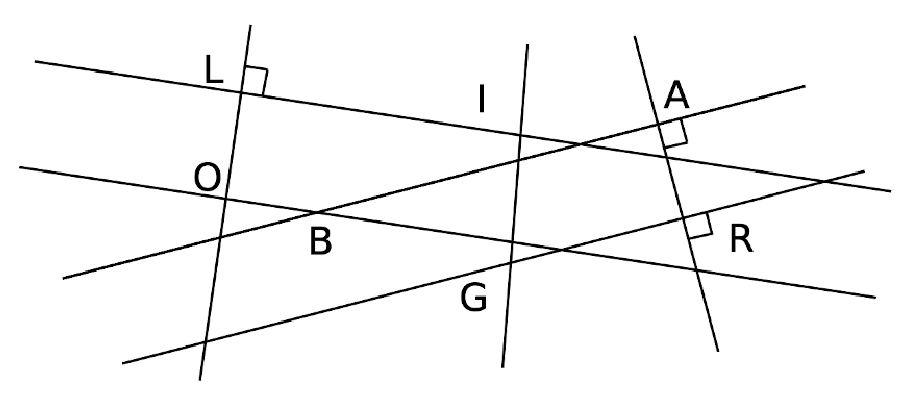
\includegraphics[width=8cm]{exercice}
   \end{center}
   \begin{enumerate}
      \item Quelles sont les droites qui sont perpendiculaires ?
      \item Quelle semble être la position relative des droites (BA) et (GR) ?
      \item Quelle est la droite perpendiculaire à la droite (GR) passant par le point A ?
      \item Quelle est la droite perpendiculaire à la droite (AR) passant par le point B ?
      \item Quelle est la droite perpendiculaire à la droite (LO) passant par le point I ?
   \end{enumerate}
\end{exercice}
\flushright{\it\footnotesize Source : Sesamath, le manuel 6\up{e}. Génération 5 - 2013}
\end{colonne*exercice}


%%%%%%%%%%%%%%%%%%%%%%%%%%%%%%%%%%%%%%%
%%%%%%%%%%%%%%%%%%%%%%%%%%%%%%%%%%%%%%%
\Recreation

\enigme[La grenouille qui saute]
   Prendre une feuille dont la longueur est deux fois plus longue que la largeur. \\
   Les plis en courts pointillés sont des plis \og vallée \fg, les plis en longs pointillés sont des plis \og montagne \fg. \\
   {\small
   \psset{linecolor=PartieStatistique}
   \begin{tabular}{p{3.8cm}p{3.8cm}p{3.8cm}p{3.8cm}}
      \begin{pspicture}(0.1,-0.25)(3.9,4.5)
         \psframe(1,0)(3,4)
         \psline[linestyle=dotted](1,2)(3,2)
         \rput(0.7,2){\textcolor{PartieStatistique}{A}}
         \rput(3.3,2){\textcolor{PartieStatistique}{B}}
      \end{pspicture}
      &
      \begin{pspicture}(0.1,-0.25)(3.9,4.5)
         \psframe(1,0)(3,4)
         \psline[linestyle=dotted](1,2)(3,2)
         \psline[linestyle=dotted](1,2)(3,4)
         \rput(0.7,2){\textcolor{PartieStatistique}{A}}
         \rput(3.3,2){\textcolor{PartieStatistique}{B}}
      \end{pspicture}
      &
      \begin{pspicture}(0.1,-0.25)(3.9,4.5)
         \psframe(1,0)(3,4)
         \psline[linestyle=dotted](1,2)(3,2)
         \psline[linestyle=dotted](1,2)(3,4)
         \psline[linestyle=dotted](1,4)(3,2)
         \psline[linestyle=dotted](1,0)(3,2)
         \psline[linestyle=dotted](1,2)(3,0)
          \rput(0.7,2){\textcolor{PartieStatistique}{A}}
         \rput(3.3,2){\textcolor{PartieStatistique}{B}}
      \end{pspicture}
      &
      \begin{pspicture}(0.1,-0.25)(3.9,4.5)
         \psframe(1,0)(3,4)
         \psline[linestyle=dotted](1,2)(3,2)
         \psline[linestyle=dotted](1,2)(3,4)
         \psline[linestyle=dotted](1,4)(3,2)
         \psline[linestyle=dotted](1,0)(3,2)
         \psline[linestyle=dotted](1,2)(3,0)
         \psline[linestyle=dashed](1,3)(3,3)
         \psline[linestyle=dashed](1,1)(3,1)
         \rput(0.7,3){\textcolor{PartieStatistique}{C}}
         \rput(3.3,3){\textcolor{PartieStatistique}{D}}
         \rput(0.7,2){\textcolor{PartieStatistique}{A}}
         \rput(3.3,2){\textcolor{PartieStatistique}{B}}
         \rput(0.7,1){\textcolor{PartieStatistique}{E}}
         \rput(3.3,1){\textcolor{PartieStatistique}{F}}
      \end{pspicture} \\
      1) Plier la feuille en deux selon la médiane la plus courte du rectangle : (AB)
      &
      2) Dans le carré du haut, plier suivant la diagonale passant par A puis déplier
      &
      3) Plier puis déplier de la même manière les trois autres diagonales
      &
      4) Plier suivant les médianes (CD) et (EF) des deux carrés \\
      \begin{pspicture}(0.1,-0.25)(3.9,3.5)
         \psframe(1,0)(3,2)
         \psline[linestyle=dotted](1,0)(3,2)
         \psline[linestyle=dotted](1,2)(3,0)
         \psline[linestyle=dashed](1,1)(3,1)
         \rput(0.7,2){\textcolor{PartieStatistique}{\footnotesize A}}
         \rput(3.3,2){\textcolor{PartieStatistique}{\footnotesize B}}
         \rput(0.7,1){\textcolor{PartieStatistique}{\footnotesize E}}
         \rput(3.3,1){\textcolor{PartieStatistique}{\footnotesize F}}      
         \psline(3,2)(2,3)(1,2)
         \psdot(2,2)
         \rput(2,1.7){\textcolor{PartieStatistique}{\footnotesize C}}
         \rput(2,2.3){\textcolor{PartieStatistique}{\footnotesize D}}    
      \end{pspicture}
      &
      \begin{pspicture}(0.1,-0.25)(3.9,3.5)
         \pspolygon(2,1)(3,2)(2,3)(1,2)
         \psline(1,2)(3,2)
         \psdot(2,2)
         \rput(1.85,1.8){\textcolor{PartieStatistique}{\footnotesize C}}
         \rput(1.85,2.2){\textcolor{PartieStatistique}{\footnotesize D}}
         \rput(2.15,1.8){\textcolor{PartieStatistique}{\footnotesize E}}
         \rput(2.15,2.2){\textcolor{PartieStatistique}{\footnotesize F}}
         \rput(0.8,2){\textcolor{PartieStatistique}{\footnotesize A}}
         \rput(3.2,2){\textcolor{PartieStatistique}{\footnotesize B}}    
      \end{pspicture}
      &
      \begin{pspicture}(0.1,-0.25)(3.9,3.5)
         \pspolygon(2,1)(3,2)(2,3)(1,2)
         \psline(1,2)(3,2)
         \psline[linestyle=dotted](2,2)(2.5,2.5)
         \rput(0.8,2){\textcolor{PartieStatistique}{\footnotesize A}}
         \rput(3.2,2){\textcolor{PartieStatistique}{\footnotesize B}}
         \rput(2,3.2){\textcolor{PartieStatistique}{\footnotesize G}}
         \psarc[linecolor=cyan]{->}(2.6,2.6){0.35}{-45}{135}
     \end{pspicture}
      &
      \begin{pspicture}(0.1,-0.25)(3.9,3.5)
         \pspolygon(2,1)(3,2)(2,3)(1,2)
         \psline(1,2)(3,2)
         \psline(2.5,1.5)(1.5,2.5)
         \psline(1.5,1.5)(2.5,2.5)
         \psline(2,1)(2,3)
      \end{pspicture} \\
      5) Joindre les points C et D l'un contre l'autre et les rabattre sur la droite (AB)
      &
      6) Faire la même chose avec les points E et F
      &
      7) Rabattre le coin B supérieur droit sur le sommet G
      &
      8) Faire de même avec les trois autres coins en A et B \\
      \begin{pspicture}(0.1,0.75)(3.9,3.5)
         \pspolygon(2,1)(3,2)(2,3)(1,2)
         \psline(1,2)(3,2)
         \psline(2.5,1.5)(1.5,2.5)
         \psline(1.5,1.5)(2.5,2.5)
         \psline(2,1)(2,3)
         \psline[linestyle=dotted](2,2)(2.29,2.71)
         \psarc[linecolor=cyan]{<-}(2.35,2.75){0.2}{-40}{130}
      \end{pspicture}
      &
      \begin{pspicture}(0.1,0.75)(3.9,3.5)
         \pspolygon(2,1)(3,2)(2,3)(1,2)
         \psline(1,2)(3,2)
         \pspolygon[fillstyle=solid,fillcolor=white](1.29,1.29)(1.71,1.29)(2.29,2.71)(2.71,2.71)
         \pspolygon[fillstyle=solid,fillcolor=white](1.29,2.71)(1.7,2.71)(2.29,1.29)(2.71,1.29)
     \end{pspicture}
      &
     \begin{pspicture}(0.1,0.75)(3.9,3.5)
         \pspolygon(1.29,1.29)(1.71,1.29)(2.29,2.71)(2.71,2.71)
         \pspolygon(1.29,2.71)(1.7,2.71)(2.29,1.29)(2.71,1.29)
         \pspolygon[fillstyle=solid,fillcolor=white](2,1)(3,2)(2,3)(1,2)
         \psline[linestyle=dotted](2,1)(2,3)
         \psline[linestyle=dashed](1,2)(3,2)
         \rput(2,3.2){\textcolor{PartieStatistique}{\footnotesize G}}
         \rput(2,0.8){\textcolor{PartieStatistique}{\footnotesize H}}
      \end{pspicture}
      &
      \begin{pspicture}(0.1,0.75)(3.9,3.5)
         \pspolygon(1.29,1.29)(1.71,1.29)(2.29,2.71)(2.71,2.71)
         \pspolygon(1.29,2.71)(1.7,2.71)(2.29,1.29)(2.71,1.29)
         \pspolygon[fillstyle=solid,fillcolor=white](2,1)(3,2)(2,3)(1,2)
         \psline[linestyle=dotted](2,1)(2,3)
         \psline[linestyle=dotted](1.42,1.58)(2,3)
         \psline[linestyle=dotted](2.58,1.58)(2,3)
         \rput(2,3.2){\textcolor{PartieStatistique}{\footnotesize G}}
         \rput(2,0.8){\textcolor{PartieStatistique}{\footnotesize H}}
         \rput(0.8,2){\textcolor{PartieStatistique}{\footnotesize B}}
         \rput(3.2,2){\textcolor{PartieStatistique}{\footnotesize A}}
         \psarc[linecolor=cyan]{<-}(2.5,2.1){0.35}{200}{-20}
         \psarc[linecolor=cyan]{->}(1.5,2.1){0.35}{200}{-20}
      \end{pspicture} \\
      9) Replier le triangle supérieur droit de manière à superposer son hypoténuse à son côté inférieur
      &
      10) Faire la même chose avec les trois autres triangles
      &
      11) Retourner la feuille, plier puis déplier suivant la diagonale (GH)
      &
      12) Amener les points A et B sur la diagonale (GH) \\ 
       \begin{pspicture}(0.1,0.75)(3.9,3.5)
         \pspolygon(1.29,1.29)(1.71,1.29)(2.29,2.71)(2.71,2.71)
         \pspolygon(1.29,2.71)(1.7,2.71)(2.29,1.29)(2.71,1.29)
         \pspolygon[fillstyle=solid,fillcolor=white](2,2)(2.5,2.5)(2,3)(1.5,2.5)
         \pspolygon[fillstyle=solid,fillcolor=white](2,1)(2.58,1.58)(2,3)(1.42,1.58)
         \psline[linestyle=dotted](2,1)(2,1.58)
         \psline(2,1.58)(2,3)
         \psline(1.42,1.58)(2.58,1.58)
         \psline(1.58,2)(2,1.58)(2.42,2)
         \psline[linestyle=dotted](1.5,1.48)(2.5,1.48)
         \psarc[linecolor=cyan]{<-}(1.9,1.58){0.5}{80}{-80}
      \end{pspicture}
      &
      \begin{pspicture}(0.1,0.75)(3.9,3.5)
         \pspolygon(1.29,1.29)(1.71,1.29)(2.29,2.71)(2.71,2.71)
         \pspolygon(1.29,2.71)(1.7,2.71)(2.29,1.29)(2.71,1.29)
         \pspolygon[fillstyle=solid,fillcolor=white](2,2)(2.5,2.5)(2,3)(1.5,2.5)
         \pspolygon[fillstyle=solid,fillcolor=white](1.5,1.5)(2.5,1.5)(2.58,1.58)(2,3)(1.42,1.58)
         \psline(2,1.58)(2,3)
         \psline(1.42,1.58)(2.58,1.58)
         \psline(1.58,2)(2,1.58)(2.42,2)
         \pspolygon[fillstyle=solid,fillcolor=white](1.5,1.5)(2.5,1.5)(2,2)
         \psline(1.71,1.29)(1.5,1.5)
         \psline(2.29,1.29)(2.5,1.5)
         \psline[linecolor=cyan]{->}(1.7,2.1)(1.95,1.7)
         \psline[linecolor=cyan]{->}(2.3,2.1)(2.05,1.7)
      \end{pspicture}
      &
      \begin{pspicture}(0.1,0.75)(3.9,3.5)
         \pspolygon(1.29,1.29)(1.71,1.29)(2.29,2.71)(2.71,2.71)
         \pspolygon(1.29,2.71)(1.7,2.71)(2.29,1.29)(2.71,1.29)
         \pspolygon[fillstyle=solid,fillcolor=white](2,2)(2.5,2.5)(2,3)(1.5,2.5)
         \pspolygon[fillstyle=solid,fillcolor=white](1.5,1.5)(2.5,1.5)(2.58,1.58)(2,3)(1.42,1.58)
         \psline(2,1.58)(2,3)
         \psline(1.42,1.58)(2.58,1.58)
         \psline(1.58,2)(2,1.58)(2.42,2)
         \pspolygon[fillstyle=solid,fillcolor=white](1.5,1.5)(2.5,1.5)(2,2)
         \psline(1.71,1.29)(1.5,1.5)
         \psline(2.29,1.29)(2.5,1.5)
        \psline[linestyle=dashed](1.58,2)(2.42,2)
         \psline[linestyle=dotted](1.48,1.75)(2.52,1.75)
         \psarc[linecolor=cyan]{<-}(2.9,1.7){0.15}{80}{-80}
         \psarc[linecolor=cyan]{->}(2.7,2.1){0.15}{-100}{100}
      \end{pspicture}
      &
      \begin{pspicture}(0.1,0.75)(3.9,3.5)
         \pspolygon(2,2.05)(2.29,2.71)(2.71,2.71)
         \pspolygon(1.29,2.71)(1.7,2.71)(2,2.05)
         \pspolygon(1.48,2.24)(2.52,2.24)(2.42,2)(1.58,2)
        \pspolygon(1.48,2.24)(1.41,2.08)(1.5,2)(2.5,2)(2.59,2.08)(2.52,2.24)
         \psline(1.41,2.08)(1.54,2.08)
         \psline(2.59,2.08)(2.46,2.08)
         \psline(1.5,2)(1.55,2.06)
         \psline(2.5,2)(2.45,2.06)      
         \pspolygon[fillstyle=solid,fillcolor=white](2,2)(2.5,2.5)(2,3)(1.5,2.5)
         \pspolygon[fillstyle=solid,fillcolor=white](1.58,2)(2,3)(2.42,2)
         \psline(2,2)(2,3)
         \psline(1.79,2)(1.72,1.79)(1.5,2)(1.32,1.79)(1.72,1.79)
         \psline(2.21,2)(2.28,1.79)(2.5,2)(2.68,1.79)(2.28,1.79)  
      \end{pspicture}
       \\
      13) Plier le triangle inférieur au niveau des pattes de derrière
      &
      14) Rentrer les coins dans les encoches du triangle plié
      &
      15) Faire un pli montagne au niveau du sommet du triangle inférieur puis un pli vallée entre ce pli et la base &
      16) On obtient une jolie grenouille\dots{} ou pas ! \\
   \end{tabular}}

   Il ne reste plus qu'à décorer la grenouille ;-)

%\enigme[Pythagorea]
%   \partie[introduction]
%      {\bf Pythagorea} est un jeu géométrique qui propose de résoudre des problèmes à l’aide d’un quadrillage de manière graduée. Les notions abordées trouvent des applications dans toutes les classes de collège notamment : longueurs et distances, parallèles, triangles isocèles, médianes et milieux, symétrie axiale, perpendiculaires, parallélogrammes, trapèzes, carrés, cercles, symétrie centrale, théorème de Pythagore, longueurs et proportions, aire, triangles rectangles, hauteurs, losanges, rotation, angles\dots). \\
%      Il est possible de le télécharger gratuitement sur smartphones et tablettes sur l'\href{https://apps.apple.com/fr/app/pythagorea/id994864779}{App Store}{} ou sur \href{https://play.google.com/store/apps/details?id=com.hil_hk.pythagorea&hl=fr}{Google Play}.
%      
%   \partie[jouons !]
%      Deux \og thèmes \fg{} du jeu se rapportent à ce chapitre, il s'agit du thème 2 : Parallèles et du thème 6 : Perpendiculaires. \\
%      Voici résumé dans ce tableau les différentes \og missions \fg{} que l'on demande de résoudre :
%      \begin{center}
%         \begin{tabular}{|C{5}|C{5}|C{5}|}
%            \hline
%            \multicolumn{3}{|c|}{\bf Droites parallèles} \\
%            \hline
%            Construire une droite parallèle à une droite existante passant par un point donné. & Sélectionner deux droites parallèles parmi des droites données. & Construire deux droites parallèles passant par des paires de points donnés. \\
%            \includegraphics[width=4cm]{pythagorea_a1} & \includegraphics[width=4cm]{pythagorea_a2} & \includegraphics[width=4cm]{pythagorea_a3} \\
%            \hline
%            \hline
%            \multicolumn{3}{|c|}{\bf Droites perpendiculaires} \\
%            \hline
%            Construire une droite perpendiculaire à une droite existante passant par un point donné. & Sélectionner deux droites perpendiculaires parmi des droites données. & Construire deux droites perpendiculaires passant par des paires de points donnés. \\
%            \includegraphics[width=4cm]{pythagorea_e1} & \includegraphics[width=4cm]{pythagorea_e2} & \includegraphics[width=4cm]{pythagorea_e3} \\
%            \hline
%         \end{tabular}
%      \end{center}
 

\themaN
\graphicspath{{../Ch4_Relations_d_ordre_sur_les_nombres/Images/}}

\chapter{Comparer\\des décimaux}
\label{C05}


%%%%%%%%%%%%%%%%%%%%%%%%%%%%%%%%%%%%%
\begin{prerequis}[Connaissances et compétences abordées]
   \begin{itemize}
      \item Repérer et placer un nombre décimal sur une demi-droite graduée adaptée.
      \item Comparer, ranger des nombres décimaux.
      \item Encadrer un nombre décimal par deux nombres entiers, par deux nombres décimaux.
      \item Trouver des nombres décimaux à intercaler entre deux nombres donnés.
      \item Connaître des procédures élémentaires de calcul, notamment : multiplier ou diviser un nombre décimal par 10, par 100, par 1000;
   \end{itemize}
\end{prerequis}

\vfill

\begin{debat}[Débat : vrai ou faux ?]
   \begin{enumerate}
      \item $4,26<4,249$ \hfill vrai \psframe(0,0)(0.25,0.25) \qquad faux \psframe(0,0)(0.25,0.25) \qquad \textcolor{white}{espace}
      \item $1,4 =1,40$ \hfill vrai \psframe(0,0)(0.25,0.25) \qquad faux \psframe(0,0)(0.25,0.25) \qquad \textcolor{white}{espace}
      \item 2,47 est le successeur de 2,46 \hfill vrai \psframe(0,0)(0.25,0.25) \qquad faux \psframe(0,0)(0.25,0.25) \qquad \textcolor{white}{espace}
      \item $2,3+7,12 =9,15$ \hfill vrai \psframe(0,0)(0.25,0.25) \qquad faux \psframe(0,0)(0.25,0.25) \qquad \textcolor{white}{espace}
      \item Entre 5 et 8, il y a une infinité de nombres décimaux \hfill vrai \psframe(0,0)(0.25,0.25) \qquad faux \psframe(0,0)(0.25,0.25) \qquad \textcolor{white}{espace}
   \end{enumerate}
   \bigskip
   \begin{center}
      \textcolor{B1}{\huge $1,11111>1,1111>1,111>1,11>1,1>1$}
   \end{center}
   \bigskip
   \begin{cadre}[B2][F4]
      \begin{center}
         Vidéo : \href{https://lesfondamentaux.reseau-canope.fr/discipline/mathematiques/nombres/comparer-les-decimaux/ranger-des-nombres.html}{\bf Ranger des nombres} du site {\it Canopé}, épisode de la série {\it Les fondamentaux}
      \end{center}
   \end{cadre}
\end{debat}

\vfill

\textcolor{PartieGeometrie}{\large\sffamily\bfseries Cahier de compétences} : chapitre 2, exercices 22 à 39.


%%%%%%%%%%%%%%%%%%%%%%%%%%%%%%%%%%%%
%%%%%%%%%%%%%%%%%%%%%%%%%%%%%%%%%%%%%
\activites

\begin{activite}[Avec une droite graduée, le retour !]
   {\bf Objectifs :} comparer, ordonner, encadrer, intercaler des nombres décimaux.
   \begin{QCM}
      \partie[réinvestissement]
         Reprendre la bande graduée du chapitre 3. \\
         Rappeler oralement la manière dont a été construire la graduation de la bande graduée. \\
         Quels sont les nombres qui ont été placés sur cette droite ? \\ [3mm]
         \pf \\ [5mm]
         \pf \\
         
      \partie[ordonner, encadrer, intercaler des nombres décimaux]
      
         \begin{enumerate}
            \item Écrire dans l'ordre croissant les nombres inscrits sur la droite graduée : \\ [3mm]
               \pf \\ [5mm]
               \pf \\
            \item Encadrer chacun des nombres suivants par deux nombres entiers consécutifs. \\
            \begin{colitemize}{3}
               \item \pfh < $\dfrac{8}{10}$ < \pfh \bigskip
               \item \pfh < 0,3 < \dashrulefill[0.5mm]{4 2}{0.15}  \bigskip
               \item \pfh < {\small cinq dixièmes} < \pfh \bigskip
               \item \pfh < $\dfrac{23}{10}$ < \pfh  \bigskip
               \item \pfh < 1,7 < \pfh
               \item \pfh < $2+\dfrac{1}{10}$ < \pfh
               \item \pfh < {\small douze dixièmes} < \pfh
               \item \pfh < $\dfrac{143}{100}$ < \pfh
               \item \pfh < $\dfrac{255}{100}$ < \pfh
               \item \pfh < 0,23 < \pfh
               \item \pfh < {\small 106 centièmes} < \pfh
               \item \pfh < $1+\dfrac{9}{10}+\dfrac{8}{100}$ < \pfh
            \end{colitemize}
            \item Encadrer chacun des nombres suivants par deux nombres décimaux séparés d'un dixième. \\
            \begin{colitemize}{3}
               \item \pfh < $\dfrac{143}{100}$ < \pfh \bigskip
               \item \pfh < $\dfrac{255}{100}$ < \pfh \bigskip
               \item \pfh < 0,23 < \pfh
               \item \pfh < {\small 106 centièmes} < \pfh
               \item \pfh < $1+\dfrac{9}{10}+\dfrac{8}{100}$ < \pfh
            \end{colitemize}
            \item \, Intercaler trois nombres entre : \medskip
            \begin{itemize}
               \item cinq dixièmes et $\dfrac{8}{10}$ : \pfb \\
               \item 2 et $2+\dfrac{1}{10}$ : \pfb \\
               \item 0,23 et 0,3 : \pfb
            \end{itemize}
         \end{enumerate}
   \end{QCM}
\end{activite}


%%%%%%%%%%%%%%%%%%%%%%%%%%%%%%%%%
%%%%%%%%%%%%%%%%% III %%%%%%%%%%%%%%%
\cours

\section{La droite graduée}

Si on partage l'unité d'une droite graduée en dix, on obtient des dixièmes; en partageant un dixième en dix, on obtient des centièmes \dots
      
\begin{center}   
   \begin{pspicture}(-2,-3)(11,1)
   {\psset{yunit=0.7}
      \small
      \rput(0,-1){
\includegraphics[width=3cm]{loupe}}
      \psaxes[yAxis=false]{->}(0,0)(10.3,0)
      \multido{\n=0.1+0.1}{9}{\psline[linewidth=0.01,linecolor=A1](\n,0.08)(\n,-0.08)}
      \psline[linestyle=dashed,linecolor=A1]{->}(0,0)(0,-2)
      \psline[linestyle=dashed,linecolor=A1]{->}(1,0)(10,-2)
      \psaxes[Dx=0.1,dx=1,comma,yAxis=false,linecolor=A1]{->}(0,-2)(10.3,-2)
      \multido{\n=0.1+0.1}{9}{\psline[linewidth=0.01,linecolor=B1](\n,-1.92)(\n,-2.08)}
      \psline[linestyle=dashed,linecolor=B1]{->}(0,-2)(0,-4)
      \psline[linestyle=dashed,linecolor=B1]{->}(1,-2)(10,-4)
      \psaxes[Dx=0.01,dx=1,comma,yAxis=false,linecolor=B1]{->}(0,-4)(10.3,-4)
      \multido{\n=0.1+0.1}{9}{\psline[linewidth=0.01](\n,-3.92)(\n,-4.08)}}
   \end{pspicture}
\end{center}


%%%%%%%%%%%%%%%%% III %%%%%%%%%%%%%%%
\section{Comparer des nombres décimaux}

\begin{methode}[Comparaison de deux nombres décimaux]
   Pour comparer deux nombres décimaux :
   \begin{itemize}
      \item je compare les parties entières ;
      \item si les parties entières sont égales, alors je compare les chiffres des dixièmes ;
      \item si les chiffres des dixièmes sont égaux, alors je compare les chiffres des centièmes et ainsi de suite jusqu’à ce que les deux nombres aient des chiffres différents.
   \end{itemize}
   \exercice
      Comparer 4,735 et 4, 74.  
   \correction
      Ils ont même partie entière, même chiffre des dixièmes mais un chiffre des centièmes différent : $3<4$ don $4,735<4,74$.
\end{methode}


%%%%%%%%%%%%%%%%%%%%%%%%%%%%%%%%%
\section{Ranger, encadrer, intercaler}

Tout comme les nombres entiers, on peut ranger, encadrer, intercaler des nombres décimaux.

\begin{exemple*1}
   \begin{itemize}
      \item $8,37<8,6<8,7$ sont rangés dans l'ordre croissant.
      \item $8,7>8,6>8,37$ sont rangés dans l'ordre décroissant.
      \item On peut encadrer $8,37$ par deux entiers consécutifs : $8<8,37<9$.
      \item On peut intercaler un nombre entre 8,6 et 8,7 : par exemple 8,63. \\
        \begin{pspicture}(0,-0.3)(11,0.7)
           {\psset{xunit=1.3}
           \small
           \rput(10,-0.45){9}
           \rput(10,0){|}
           \psaxes[yAxis=false,Ox=8,Dx=0.1,dx=1,comma,subticks=10]{->}(0,0)(10.15,0)
           \psline[linewidth=0.05,linecolor=violet,linestyle=dashed]{->}(0,0.5)(0,0)
           \psline[linewidth=0.05,linecolor=violet]{->}(3.7,0.5)(3.7,0) 
           \psline[linewidth=0.05,linecolor=violet,linestyle=dashed]{->}(10,0.5)(10,0)
           \psline[linewidth=0.05,linecolor=teal]{->}(7,0.5)(7,0)
           \psline[linewidth=0.05,linecolor=teal,linestyle=dashed]{->}(6.3,0.5)(6.3,0)
           \psline[linewidth=0.05,linecolor=teal]{->}(6,0.5)(6,0)}
        \end{pspicture}
   \end{itemize}
\end{exemple*1}

\begin{remarque}
   on peut intercaler autant de nombres que l'on veut entre deux nombres décimaux (on dit qu'il y en a une infinité). \\
   Par exemple, entre 8,6 et 8,7 on a 8,63, mais aussi 8,64 ; 8,699 ; 8, 675344355\dots
\end{remarque}


%%%%%%%%%%%%%%%%%%%%%%%%%%%%%%%%%%%%%%%%%%
\exercicesbase

\begin{colonne*exercice}

\serie{La droite graduée} %%%%%%%%%%%%%%%%%%%%

\begin{exercice} %1
   Écrire l'abscisse de chaque point.
   \begin{enumerate}
      \small
      \item \begin{pspicture}(0,0)(8,0.7)
                  \psset{xunit=5}
                  \psaxes[yAxis=false,subticks=10,subtickcolor=black]{->}(0,0)(1.5,0)
                  \pstGeonode[PosAngle=90](0.3,0){A}(0.8,0){B}(1.1,0){C}(1.3,0){D}
               \end{pspicture}
      \item \begin{pspicture}(0,0)(8,1.2)
                  \psset{xunit=5}
                  \psaxes[yAxis=false,Ox=12,subticks=10,subtickcolor=black]{->}(0.2,0)(1.5,0)
                  \psline(0,0)(0.2,0)
                  \psline[linewidth=0.07mm](0.1,0.1)(0.1,-0.1)
                  \pstGeonode[PosAngle=90](0.3,0){E}(0.5,0){F}(0.7,0){G}(1.3,0){H}
               \end{pspicture}
      \item \begin{pspicture}(0,0)(8,1.2)
                  \psset{xunit=1.1}
                  \psaxes[yAxis=false,Ox=24,subticks=2,subtickcolor=black,labels=none]{->}(0,0)(6.5,0)
                  \rput(1,-0.3){25}
                  \rput(2,-0.3){26}
                  \psline(0,0)(0.2,0)
                  \psline[linewidth=0.07mm](0.1,0.1)(0.1,-0.1)
                  \pstGeonode[PosAngle=90](1.5,0){J}(3.5,0){K}(5.5,0){L}
               \end{pspicture}
      \item \begin{pspicture}(0,0)(8,1.2)
                  \psset{xunit=0.45}
                  \psline{->}(0,0)(16,0)
                  \multido{\n=1+1}{15}{\psline[linecolor=darkgray,linewidth=0.1mm](\n,-0.1)(\n,0.1)}
                  \psline(2,-0.1)(2,0.1)
                  \rput(2,-0.35){7,8}
                  \psline(12,-0.1)(12,0.1)
                  \rput(12,-0.35){7,9}
                  \pstGeonode[PosAngle=90](3,0){M}(5,0){N}(11,0){P}(13,0){Q}
               \end{pspicture}
       \item \begin{pspicture}(0,0)(8,1.2)
                  \psset{xunit=0.45}
                  \psline{->}(0,0)(16,0)
                  \multido{\n=1+1}{15}{\psline[linecolor=darkgray,linewidth=0.1mm](\n,-0.1)(\n,0.1)}
                  \psline(4,-0.1)(4,0.1)
                  \rput(4,-0.35){6,41}
                  \psline(14,-0.1)(14,0.1)
                  \rput(14,-0.35){6,42}
                  \pstGeonode[PosAngle=90](2,0){V}(7,0){W}(10,0){Y}(12,0){Z}
               \end{pspicture}
   \end{enumerate}
\end{exercice}

%\begin{corrige}
%   \ \\ [-5mm]
%   \begin{enumerate}
%      \item $A({\blue 0,3}) \; ; \; B({\blue 0,8}) \; ; \; C({\blue 1,1}) \; ; \; D({\blue 1,3})$.
%      \item $E({\blue 12,1}) \; ; \; F({\blue 12,3}) \; ; \; G({\blue 12,5}) \; ; \; H({\blue 13,1})$.
%      \item $J({\blue 25,5}) \; ; \; K({\blue 27,5}) \; ; \; L({\blue 29,5})$.
%      \item $M({\blue 7,81}) \; ; \; N({\blue 7,83}) \; ; \; P({\blue 7,89}) \; ; \; Q({\blue 7,91})$.
%      \item $V({\blue 6,408}) \; ; \; W({\blue 6,413}) \; ; \; Y({\blue 6,416}) \; ; \; Z({\blue 6,418})$.
%   \end{enumerate}
%\end{corrige}

\bigskip

\begin{exercice}
   Placer les points donnés sur chaque droite.
   {\psset{unit=0.9}
   \small
   \begin{enumerate}
      \item A(11,5) \; ; \; B(8,5) \; ; \; C(9,7) \; et \; D(8,1). \\
        \begin{pspicture}(0.3,-0.5)(8,1.2)
           \milli{0}{-0.5}{8}{1}
           \psaxes[yAxis=false,Dx=2,labels=none]{->}(0,0)(8,0)
           \rput(2,-0.35){9}
           \rput(4,-0.35){10}
        \end{pspicture}
      \item E(0,2) \; ; \; F(0,55) \; ; \; G(0,73) \; et \; H(0,40). \\
        \begin{pspicture}(0.3,-0.5)(8,1.2)
           \milli{0}{-0.5}{8}{1}
           \psaxes[yAxis=false,labels=none]{->}(0,0)(8,0)
           \rput(2,-0.35){0,3}
           \rput(3,-0.35){0,4}
        \end{pspicture}
     \item J(5,33) \; ; \; K(5,28) \; ; \; L(5,315) \; et \; M(5,304). \\
        \begin{pspicture}(0.3,-0.5)(8,1.2)
           \milli{0}{-0.5}{8}{1}
           \psaxes[yAxis=false,Dx=1,labels=none]{->}(0,0)(8,0)
           \rput(3,-0.35){5,3}
           \rput(4,-0.35){5,31}
        \end{pspicture}
   \end{enumerate}}
\end{exercice}


\serie{Comparer des nombre décimaux} %%%%%%%%%%%%%


\medskip

\begin{exercice} %3
   Compléter avec le signe < ou >. \medskip
   \begin{colenumerate}{2}
      \item 15,1 \pfh 15,09 \smallskip
      \item 132,45 \pfh 132,46 \smallskip
      \item 7,101 \pfh 17,011 \smallskip
      \item 435,6 \pfh 438,6
      \item 5,126 \pfh 5,1236
      \item 6,048 \pfh 6,15
   \end{colenumerate}
\end{exercice}

%\begin{corrige}
%   \begin{colenumerate}{2}
%      \item 15,1 {\blue\,>\,} 15,09 \smallskip
%      \item 132,45 {\blue\,<\,} 132,46 \smallskip
%      \item 7,101 {\blue\,>\,} 17,011 \smallskip
%      \item 435,6 {\blue\,<\,} 438,6 \smallskip
%      \item 5,126 {\blue\,>\,} 5,1236
%      \item 6,048 {\blue\,<\,} 6,15
%      \item 8,75 {\blue\,<\,} 8,9
%      \item 19,47 {\blue\,>\,} 19,435
%   \end{colenumerate}
%\end{corrige}

\begin{exercice} %2
   Compléter avec le signe < ou >. \medskip
   \begin{colenumerate}{2}
      \item $\dfrac{32}{100} \pfh \dfrac{40}{100}$ \medskip
      \item $\dfrac{7}{10} \pfh \dfrac{7}{100}$ \medskip
      \item $\dfrac{43}{100} \pfh \dfrac{4}{10}$ \medskip
      \item $\dfrac{37}{100} \pfh \dfrac{307}{1\,000}$
      \item $5+\dfrac{8}{10} \pfh 5+\dfrac{8}{100}$
      \item $3+\dfrac{2}{10} \pfh 3+\dfrac{22}{100}$
   \end{colenumerate}
\end{exercice}

%\begin{corrige}
%   \begin{colenumerate}{2}
%      \item $\dfrac{32}{100} {\blue\,<\,} \dfrac{40}{100}$ \medskip
%      \item $\dfrac{7}{10} {\blue\,>\,} \dfrac{7}{100}$ \medskip
%      \item $\dfrac{43}{100} {\blue\,>\,} \dfrac{4}{10}$ \medskip
%      \item $\dfrac{85}{100} {\blue\,<\,} \dfrac{9}{10}$
%      \item $\dfrac{37}{100} {\blue\,>\,} \dfrac{307}{1\,000}$
%      \item $5+\dfrac{8}{10} {\blue\,>\,} 5+\dfrac{8}{100}$
%      \item $3+\dfrac{2}{10} {\blue\,<\,} 3+\dfrac{22}{100}$
%      \item $\dfrac{7\,859}{1\,000} {\blue\,<\,} 78+\dfrac{59}{100}$
%   \end{colenumerate}
%\end{corrige}


\serie{Ranger, encadrer, intercaler} %%%%%%%%%%%%%%%%%%

\begin{exercice}
   Ranger chaque série de nombres :
   \begin{enumerate}
      \item dans l'ordre croissant. \smallskip
      \begin{enumerate}
         \item \fbox{4,99} \; \fbox{4,9} \; \fbox{4,88} \; \fbox{5,01} \; \fbox{4,909} \; \fbox{4,879} \smallskip
         \item \fbox{0,7} \; \fbox{0,07} \; \fbox{0,707} \; \fbox{0,007} \; \fbox{0,77} \; \fbox{0,077}
      \end{enumerate}
      \item dans l'ordre décroissant. \smallskip
      \begin{enumerate}
         \item \fbox{1,28} \; \fbox{1,82} \; \fbox{1,028} \; \fbox{1,8} \; \fbox{1,282} \; \fbox{1,2} \smallskip
         \item \fbox{5,3} \; \fbox{3,5} \; \fbox{5,35} \; \fbox{3,53} \; \fbox{5,353} \; \fbox{3,535}
      \end{enumerate}
   \end{enumerate}
\end{exercice}

%\begin{corrige}
%   \ \\ [-5mm]
%   \begin{enumerate}
%      \item \blue 0,007 \, < \, 0,07 \, < \, 0,077 \, < \, 0,7 \, < \, 0,707 \, < \, 0,77
%      \item 5,353 \, > \, 5,35 \, > \, 5,3 \, > \, 3,535 \, > \, 3,53 \, > \, 3,5
%   \end{enumerate}
%\end{corrige}

\begin{exercice} %17
   Classer dans l'ordre croissant l'ensemble de ces lettres afin de trouver le mot mystère.
   \begin{colitemize}{3}
      \item I = 65,165
      \item S = $\dfrac{655}{10}$
      \item B = $\dfrac{6\,503}{100}$
   \end{colitemize}
   \begin{colitemize}{2}
      \item A = $56+\dfrac{6}{100}$
      \item M = $50+6+\dfrac{65}{1\,000}$
      \item O = $\dfrac{651}{10}+\dfrac{3}{100}$
      \item R = $56+\dfrac{5}{100}$
   \end{colitemize}
   \begin{colitemize}{1}
      \item E = $(6\times10)+(5\times1)+(6\times0,1)$
      \item F = 56 unités et 6 millièmes
   \end{colitemize}
\end{exercice}
%
%\begin{corrige}
%   \begin{colitemize}{3}
%      \item I = 65,165
%      \item S = 65,5
%      \item B = 65,03
%      \item A = 56,06
%      \item O = 65,13
%      \item M = 56,065
%      \item R = 56,05
%      \item E = 65,6
%      \item F = 56,006
%   \end{colitemize}
%   On a $65,006 < 56,05 < 56,06 < 56,065 < 65,03 < 65,13 < 65,165 < 65,5 < 65,6$. \\
%   Conclusion : le mot mystère est \blue FRAMBOISE.
%\end{corrige}

\medskip

\begin{exercice} %5
   Encadrer ces nombres par deux nombres décimaux séparés d'un dixième.
   \begin{colenumerate}{2}
      \item \pfh < 8,51 < \pfh
      \item \pfh < 99,01 < \pfh
      \item \pfh < 0,956 < \pfh
      \item \pfh < 29,108 < \pfh
      \item \pfh < 123,19 < \pfh
      \item \pfh < 77,777 < \pfh
   \end{colenumerate}
\end{exercice}

%\begin{corrige}
%   \begin{colenumerate}{2}
%      \item {\blue 8,5} < 8,51 < {\blue 8,6}
%      \item {\blue 99} < 99,01 < {\blue 99,1}
%      \item {\blue 0,9} < 0,956 < {\blue 1}
%      \item {\blue 29,1} < 29,108 < {\blue 29,2}
%      \item {\blue 123,1} < 123,19 < {\blue 123,2}
%      \item {\blue 77,7} < 77,777 < {\blue 77,8}
%   \end{colenumerate}
%\end{corrige}

\medskip


\begin{exercice} %10
   Intercaler un nombre décimal entre les deux nombres donnés.
   \begin{colenumerate}{2}
      \item 57 < \pfh < 58
      \item 0,6 < \pfh < 0,61
      \item 8,4 < \pfh < 8,5
      \item 5,12 < \pfh < 5,123
      \item 74,1 < \pfh < 74,2
      \item 45,78 < \pfh < 45,781
   \end{colenumerate}
\end{exercice}

%\begin{corrige}
%   On a, par exemple (solutions non uniques) :
%   \begin{colenumerate}{2}
%      \item 57 < {\blue 57,5} < 58
%      \item 0,6 < {\blue 0,607} < 0,61
%      \item 8,4 < {\blue 8,41} < 8,5
%      \item 5,12 < {\blue 5,122} < 5,123
%      \item 74,1 < {\blue 74,13} < 74,2
%      \item {\small 45,78 < {\blue 45,7806} < 45,781}
%   \end{colenumerate}
%\end{corrige}

\medskip


\begin{exercice} %12
   Quel pingouin vérifie les caractéristiques suivantes (justifier) :
   \begin{itemize}
      \item il mesure entre \um{0,75} et \um{0,85} ;
      \item il pèse entre \ukg{4,8} et \ukg{5,2} ;
      \item il a moins de 10 ans.
   \end{itemize}
  \begin{center}
      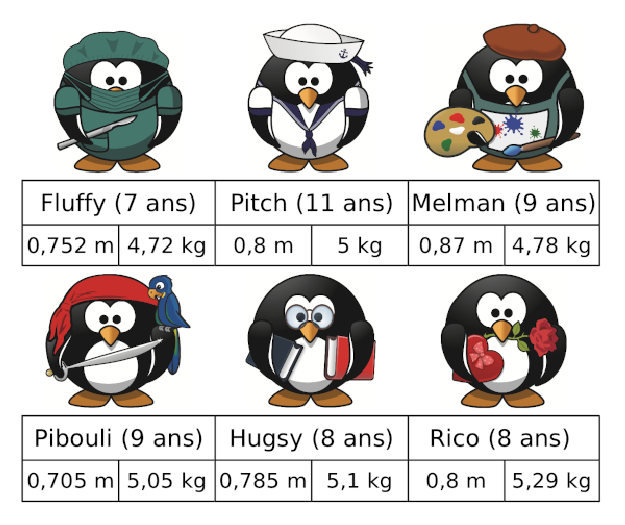
\includegraphics[width=5.5cm]{pingouin}
   \end{center}
\end{exercice}

%\begin{corrige}
%   \begin{itemize}
%      \item Le pingouin doit mesurer entre \um{0,75} et \um{0,85} donc, on peut éliminer Melman et Pibouli.
%      \item Le pingouin doit peser entre \ukg{4,8} et \ukg{5,2} donc, on peut éliminer Fluffy, Melman et Rico.
%      \item Le pingouin doit avoir moins de 10 ans donc, on peut éliminer Pitch.
%   \end{itemize}
%   Conclusion : {\blue on choisit Hugsy}. \\
%\end{corrige}

\end{colonne*exercice}


%%%%%%%%%%%%%%%%%%%%%%%%%%%%%%%%%%%%%%%
%%%%%%%%%%%%%%%%%%%%%%%%%%%%%%%%%%%%%%%
\Recreation

\enigme[Nombres croisés]
   \partie[mode d'emploi]
      Une grille de nombres croisés se comporte comme une grille de mots croisés :
      \begin{itemize}
         \item horizontalement, les lignes sont repérées par des chiffres romains de I à V ;
         \item verticalement, les colonnes sont repérées par des lettres de A à E ;
         \item les indications des nombres à trouver sont indiquées sous la grille de nombres croisés, repérées par des chiffres romains ou des lettres selon s'ils sont horizontaux ou verticaux ;
         \item il est interdit d'écrire dans les cases noires ;
         \item lorsqu'une ligne ou une colonne ne possède pas de carré noir, il y a un seul nombre à écrire ;
         \item lorsqu'une ligne ou une colonne possède un carré noir, il y a deux nombres à écrire, ces deux nombres sont définis par deux lignes différentes. \\
      \end{itemize}
      
   \partie[let's go !]
Compléter la grille à l'aide de nombres entiers correspondant aux définitions.
   \begin{center}
      {\psset{unit=1.2}\begin{pspicture}(-1,-0.5)(5,5.8)
         \psgrid[gridlabels=0,subgriddiv=0](0,0)(5,5)
         \psframe[fillstyle=solid,fillcolor=black](0,0)(1,1)
         \psframe[fillstyle=solid,fillcolor=black](4,1)(5,2)
         \psframe[fillstyle=solid,fillcolor=black](1,2)(2,3)
         \psframe[fillstyle=solid,fillcolor=black](3,4)(4,5)
         \rput(0.5,5.4){\bf A}
         \rput(1.5,5.4){\bf B}
         \rput(2.5,5.4){\bf C}
         \rput(3.5,5.4){\bf D}
         \rput(4.5,5.4){\bf E}
         \rput(-0.4,0.5){\bf V}
         \rput(-0.4,1.5){\bf IV}
         \rput(-0.4,2.5){\bf III}
         \rput(-0.4,3.5){\bf II}
         \rput(-0.4,4.5){\bf I}
      \end{pspicture}}
   \end{center}
   \begin{multicols}{2}
      {\bf Horizontalement} \\ [3mm]
         {\bf I} : Partie entière de 328,54. \\
         \hspace*{2.7mm} Chiffre des centièmes de 634,152. \\ [2mm]
         {\bf II} : Son chiffre des dizaines est le triple \\
         \hspace*{4mm} de celui des unités. \\ [2mm]
         {\bf III} : Chiffre des dixièmes de 34. \\
         \hspace*{5.6mm} Entier précédant 178,356. \\ [2mm]
         {\bf IV} : Entier compris entre 8\,000 et 9\,000. \\ [2mm]
         {\bf V} : Quarante-deux centaines. \\ [5mm]
      {\bf Verticalement} \\ [3mm]
        {\bf A} : $(3\times1 000) + (5\times100) + (8\times1)$. \\ [2mm]
        {\bf B} : Nombre de dixièmes dans 2,6. \\ [1mm]
        \hspace*{4mm} Partie entière de $\dfrac{2\,498}{100}$. \\ [3mm]
        {\bf C} : Quatre-vingt-six milliers et cent-deux unités. \\ [2mm]
        {\bf D} : En additionnant tous les chiffres \\
        \hspace*{4.5mm} du nombre, on trouve 20. \\ [2mm]
        {\bf E} : Entier qui suit 537,56. \\
        \hspace*{3.5mm} Entier qui précède 1. \\
     \end{multicols}

\themaG
\graphicspath{{../Ch6_Se_reperer_sur_un_plan_et_dans_l_espace/Images/}}

\chapter{Se repérer}
\label{C06}


%%%%%%%%%%%%%%%%%%%%%%%%%%%%%%%%%%%%%%%%%%
\begin{prerequis}[Connaissances et compétences abordées]
   \begin{itemize}
      \item Se repérer sur un plan ou sur une carte (école, quartier, ville, village).
      \item Divers modes de représentation de l’espace : maquettes, plans, schémas.
   \end{itemize}
\end{prerequis}

\vfill

\begin{debat}[Débat : le GPS] 
   GPS est l'acronyme de l'anglais \og Global Positioning System \fg{}, qui signifie \og système de positionnement global\fg. Le système comprend au moins vingt-quatre satellites émetteurs, et un nombre quasi-illimité de récepteurs. Le récepteur GPS calcule les informations émises par quatre satellites au minimum, pour obtenir les coordonnées en longitude, latitude, et altitude du point où il se trouve. Il permet de situer de manière assez précise un objet ou un personnage sur la Terre. Actuellement, la plupart des téléphones portables possèdent un GPS.
   \flushright{\footnotesize\it Source : Wikidia, l'encyclopédie des 8-13 ans}
   \begin{center}
      \begin{pspicture}(0,-0.3)(5,4.2)
         \psset{linewidth=1mm}
         \pscircle[linecolor=A1](2,2){1}
         \pscircle[linecolor=B1](3.7,1.5){1}
         \pscircle[linecolor=J1](3,3){1}
         \psline[linewidth=0.4mm,arrowsize=0.5]{->}(0,3)(2.95,2.05)
         \rput(-1,3){Je suis là !}
      \end{pspicture}
   \end{center}
   \begin{cadre}[B2][F4]
      \begin{center}
         Vidéo : \href{https://www.youtube.com/watch?v=WoqpQbWdacQ}{\bf Comment fonctionne un GPS}, chaîne YouTube {\it Unisciel}, série {\it Kezako}.
      \end{center}
   \end{cadre}
\end{debat}

\vfill

\textcolor{PartieGeometrie}{\large\sffamily\bfseries Cahier de compétences} : chapitre 1, exercices 1, 18, 20, 21, 23, 37, 40, 41, 42. 


%%%%%%%%%%%%%%%%%%%%%%%%%%%%%%%%%%%%%
%%%%%%%%%%%%%%%%%%%%%%%%%%%%%%%%%%%%%
\activites

\begin{activite}[La rose des vents]
   {\bf Objectifs :} tracer une figure géométrique précise et soignée ; suivre un programme de construction ; connaître les quatre points cardinaux.
   \begin{QCM}
         Suivre les étapes de construction de la rose des vents, la colorier, la découper et la coller dans le cours.
         {\psset{unit=0.9}
         \small
         \begin{center}
            \begin{pspicture}(-4,-4)(4,3.5)
               \psset{linewidth=0.7mm}
               \pscircle(0,0){3}
               \psline(-3,0)(3,0)
               \psline(0,-3)(0,3)
               \rput(-1.5,0.35){\ucm{3}}
               \rput(-3.7,0){\large\textcolor{B1}{\bf 1)}}
            \end{pspicture}
         \begin{pspicture}(-4,-4)(4,3.5)
            \pscircle(0,0){3}
               \psline(-3,0)(3,0)
               \psline(0,-3)(0,3)
               \psset{linewidth=0.7mm}
               \psline(3;45)(3;-135)
               \psline(3;135)(3;-45)
               \rput(-3.7,0){\large\textcolor{B1}{\bf 2)}}
            \end{pspicture}

            \begin{pspicture}(-4,-4)(4,3)
               \pscircle(0,0){3}
               \psline(-3,0)(3,0)
               \psline(0,-3)(0,3)
               \psline(3;45)(3;-135)
               \psline(3;135)(3;-45)
               \psset{linewidth=0.7mm}
               \pscircle(0,0){1}
               \pscircle(0,0){2.5}
               \rput(-0.6,0.25){\ucm{1}}
               \rput(1.5,0.25){\ucm{2,5}}
               \rput(-3.7,0){\large\textcolor{B1}{\bf 3)}}
            \end{pspicture}
            \begin{pspicture}(-4,-4)(4,3)
               \pscircle(0,0){3}
               \psline(-3,0)(3,0)
               \psline(0,-3)(0,3)
               \psline(3;45)(3;-135)
               \psline(3;135)(3;-45)
               \pscircle(0,0){1}
               \pscircle(0,0){2.5}
               \psset{linewidth=0.7mm}
               \pspolygon(0,-2.9)(1;-45)(2.9,0)(1;45)(0,2.9)(1;135)(-2.9,0)(1;-135)
               \rput(-3.7,0){\large\textcolor{B1}{\bf 4)}}
            \end{pspicture}

            \begin{pspicture}(-4,-3.3)(4,3)
               \pscircle(0,0){3}
               \psline(-3,0)(3,0)
               \psline(0,-3)(0,3)
               \psline(3;45)(3;-135)
               \psline(3;135)(3;-45)
               \pscircle(0,0){1}
               \pscircle(0,0){2.5}
               \pspolygon(0,-2.9)(1;-45)(2.9,0)(1;45)(0,2.9)(1;135)(-2.9,0)(1;-135)
               \psset{linewidth=0.7mm}
               \pspolygon(2.5;45)(0,1)(2.5;135)(-1,0)(2.5;-135)(0,-1)(2.5;-45)(1,0)
               \rput(-3.7,0){\large\textcolor{B1}{\bf 5)}}
            \end{pspicture}
            \begin{pspicture}(-4,-3.3)(4,3)
               \psset{linewidth=0.7mm}
               \pspolygon(2.5;45)(0,1)(2.5;135)(-1,0)(2.5;-135)(0,-1)(2.5;-45)(1,0)
               \pspolygon[fillstyle=solid,fillcolor=white](0,-3)(1;-45)(3,0)(1;45)(0,3)(1;135)(-3,0)(1;-135)
               \psline(-3,0)(3,0)
               \psline(0,-3)(0,3)
               \psline(2.5;45)(2.5;-135)
               \psline(2.5;135)(2.5;-45)
               \rput(-3.7,0){\large\textcolor{B1}{\bf 6)}}
            \end{pspicture}
         \end{center}}
   \end{QCM}
\end{activite}


%%%%%%%%%%%%%%%%%%%%%%%%%%%%%%%%%%%%%%
%%%%%%%%%%%%%%%%%%%%%%%%%%%%%%%%%%%%%%
\cours 

\section{Se repérer sur un quadrillage} %%%

\begin{methode*2*2}[Repérage sur un quadrillage]
Pour se repérer sur un quadrillage, on peut utiliser les {\bf coordonnées} des cases ou des n\oe uds.
   \exercice
      Quadrillage à {\bf cases}. \\
      Déterminer l'emplacement du carré et du disque. \\
      \psset{unit=0.7}
      \begin{pspicture}(-2,0)(6,6.5)
         \rput(1,1){\psgrid[gridlabels=0,subgriddiv=0](5,5)}
         \rput(1.5,0.5){A}
         \rput(2.5,0.5){B}
         \rput(3.5,0.5){C}
         \rput(4.5,0.5){D}
         \rput(5.5,0.5){E}
         \rput(0.5,0.5){\multido{\n=1+1}{5}{\rput(0,\n){\n}}}
         \pscircle[linecolor=violet,fillstyle=solid,fillcolor=violet](4.5,3.5){0.3}
         \psframe[linecolor=violet,fillstyle=solid,fillcolor=violet](2.25,4.25)(2.75,4.75)
      \end{pspicture}
   \correction
      Le carré est en B4, le disque en D3.
   \exercice
      Quadrillage à {\bf n\oe uds}. Déterminer l'emplacement du triangle et du pentagone. \\
      \psset{unit=0.7}
      \begin{pspicture}(-2,0)(6,6.5)
         \rput(1,1){\psgrid[gridlabels=0,subgriddiv=0](5,5)}
         \rput(1,0.5){A}
         \rput(2,0.5){B}
         \rput(3,0.5){C}
         \rput(4,0.5){D}
         \rput(5,0.5){E}
         \rput(6,0.5){F}
         \rput(0.5,1){\multido{\n=0+1}{6}{\rput(0,\n){\n}}}
         \psdot[linecolor=violet,linewidth=2mm,dotstyle=triangle*](3,2)
         \psdot[linecolor=violet,linewidth=1.8mm,dotstyle=pentagon*](4,6)
      \end{pspicture}
   \correction
      Triangle (C;1) et pentagone (D;5).
\end{methode*2*2}


%%%%%%%%%%%%%%%%%%%%%%%%%%%%%%%%%%%%%%%
\section{Se repérer sur un plan ou une carte}

\begin{definition}
   \begin{minipage}{8cm}
      Une {\bf rose des vents} est une figure qui indique les 4 points cardinaux : est, nord, ouest et sud et éventuellement les orientations intermédiaires.
   \end{minipage}
   \hfill
   \begin{minipage}{4cm}
      \psset{unit=0.5}
      \footnotesize
      \begin{pspicture}(-3,-4)(4,4)
         \pspolygon[fillstyle=solid,fillcolor=white](2.5;45)(0,1)(2.5;135)(-1,0)(2.5;-135)(0,-1)(2.5;-45)(1,0)
         \pspolygon[fillstyle=solid,fillcolor=white](0,-3)(1;-45)(3,0)(1;45)(0,3)(1;135)(-3,0)(1;-135)
         \psline(-3,0)(3,0)
         \psline(0,-3)(0,3)
         \psline(2.5;45)(2.5;-135)
         \psline(2.5;135)(2.5;-45)
         \rput(3.5;0){E}
         \rput(3.4;45){NE}
         \rput(3.5;90){N}
         \rput(3.4;135){NO}
         \rput(3.5;180){O}
         \rput(3.4;225){SO}
         \rput(3.5;270){S}
         \rput(3.4;315){SE}
      \end{pspicture}
   \end{minipage}
\end{definition}

\begin{center}
   \begin{minipage}{7cm}
      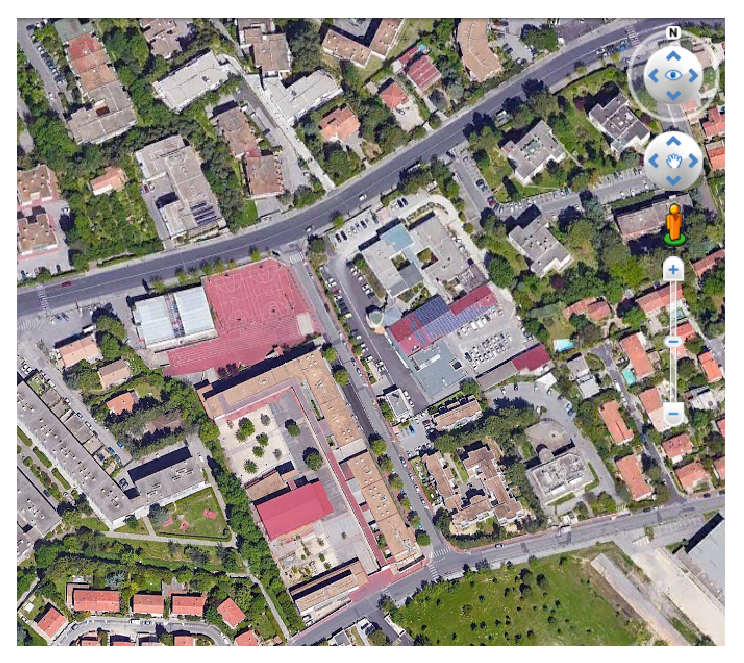
\includegraphics[width=7cm]{plan_college}
   \end{minipage}
   \qquad
   \begin{minipage}{7cm}
      Sur une carte, on peut se repérer grâce à la rose des vents, mais sur les cartes actuelles et les GPS, bien souvent, seule la direction du nord est indiquée. Elle permet à elle seule de se repérer dans le plan.
   \end{minipage}
\end{center}


%%%%%%%%%%%%%%%%%%%%%%%%%%%%%%%%%%%%%%%%%%
\exercicesbase

\begin{colonne*exercice}

\serie{Se repérer sur un quadrillage}

\begin{exercice}
   Déterminer l'emplacement des formes suivantes : \\
   \psset{unit=0.7}
   \begin{center}
      \begin{pspicture}(0,0)(8,7.5)
         \psgrid[gridlabels=0,subgriddiv=0](8,8)
         \rput(1.5,0.5){A}
         \rput(2.5,0.5){B}
         \rput(3.5,0.5){C}
         \rput(4.5,0.5){D}
         \rput(5.5,0.5){E}
         \rput(6.5,0.5){F}
         \rput(7.5,0.5){G}
         \rput(0.5,0.5){\multido{\n=1+1}{7}{\rput(0,\n){\n}}}
         \psset{linecolor=A1,linewidth=1.5mm}
         \psdot[dotstyle=triangle*](3.5,1.5)
         \psdot[dotstyle=pentagon*](4.5,6.5)
         \psdot[dotstyle=square*](1.5,2.5)
         \psdot[dotstyle=*](7.5,3.5)
         \psdot[dotstyle=diamond*](6.5,5.5)
      \end{pspicture}
   \end{center}
\end{exercice}

\begin{exercice}
   Déterminer l'emplacement des formes suivantes :  \\
   \psset{unit=0.7}
   \begin{center}
      \begin{pspicture}(0,0)(8,7.5)
         \psgrid[gridlabels=0,subgriddiv=0](1,1)(8,8)
         \rput(1,0.5){A}
         \rput(2,0.5){B}
         \rput(3,0.5){C}
         \rput(4,0.5){D}
         \rput(5,0.5){E}
         \rput(6,0.5){F}
         \rput(7,0.5){G}
         \rput(8,0.5){H}
         \rput(0.5,1){\multido{\n=0+1}{8}{\rput(0,\n){\n}}}
         \psset{linecolor=A1,linewidth=1.5mm}
         \psdot[dotstyle=triangle*](6,1)
         \psdot[dotstyle=pentagon*](2,3)
         \psdot[dotstyle=square*](1,7)
         \psdot[dotstyle=*](4,5)
         \psdot[dotstyle=diamond*](8,6)
      \end{pspicture}
   \end{center}
\end{exercice}

\begin{exercice}
   Placer les lettres suivantes dans la grille, puis vérifier en lisant de gauche à droite et de haut en bas. \\
   A $\to$ g6 ; B $\to$ b8 ; C $\to$ b4 ; E $\to$ d4 et h1 ; J $\to$ a2 ; O $\to$ h5 \\
   R $\to$ d7 ; S $\to$ b1 et f3 ; T $\to$ e1 et h3 ; U $\to$ c2 ; V $\to$ c5.
   \psset{unit=0.6}
   \begin{center}
      \begin{pspicture}(0,0)(9,9)
         \psgrid[gridlabels=0,subgriddiv=0](9,9)
         \rput(1.5,0.5){a}
         \rput(2.5,0.5){b}
         \rput(3.5,0.5){c}
         \rput(4.5,0.5){d}
         \rput(5.5,0.5){e}
         \rput(6.5,0.5){f}
         \rput(7.5,0.5){g}
         \rput(8.5,0.5){h}
         \rput(0.5,0.5){\multido{\n=1+1}{8}{\rput(0,\n){\n}}}
      \end{pspicture}
   \end{center}
\end{exercice}

\begin{exercice}
   Placer les formes suivantes dans la grille. \\
   \psset{linecolor=A1,linewidth=1.5mm}
   \hspace*{10mm} \psdot[dotstyle=*](0,0.08) \quad (d,4) \quad \psdot[dotstyle=triangle*](0,0.08) \quad (g,2) \quad \psdot[dotstyle=square*](0,0.08) \quad (a,0) \quad \psdot[dotstyle=pentagon*](0,0.08) \quad (b,6) \quad \psdot[dotstyle=diamond*](0,0.08) \quad (f,3)
   \psset{unit=0.6}
   \begin{center}
      \begin{pspicture}(0,0)(7,7)
         \psgrid[gridlabels=0,subgriddiv=0](1,1)(7,7)
         \rput(1,0.5){a}
         \rput(2,0.5){b}
         \rput(3,0.5){c}
         \rput(4,0.5){d}
         \rput(5,0.5){e}
         \rput(6,0.5){f}
         \rput(7,0.5){g}
         \rput(0.5,1){\multido{\n=0+1}{7}{\rput(0,\n){\n}}}
      \end{pspicture}
   \end{center}

\end{exercice}

\end{colonne*exercice}

\serie{Se repérer sur un plan ou une carte}

\begin{exercice}
   Voici le plan d'une cabine d'un Boeing 767.
   \begin{center}
      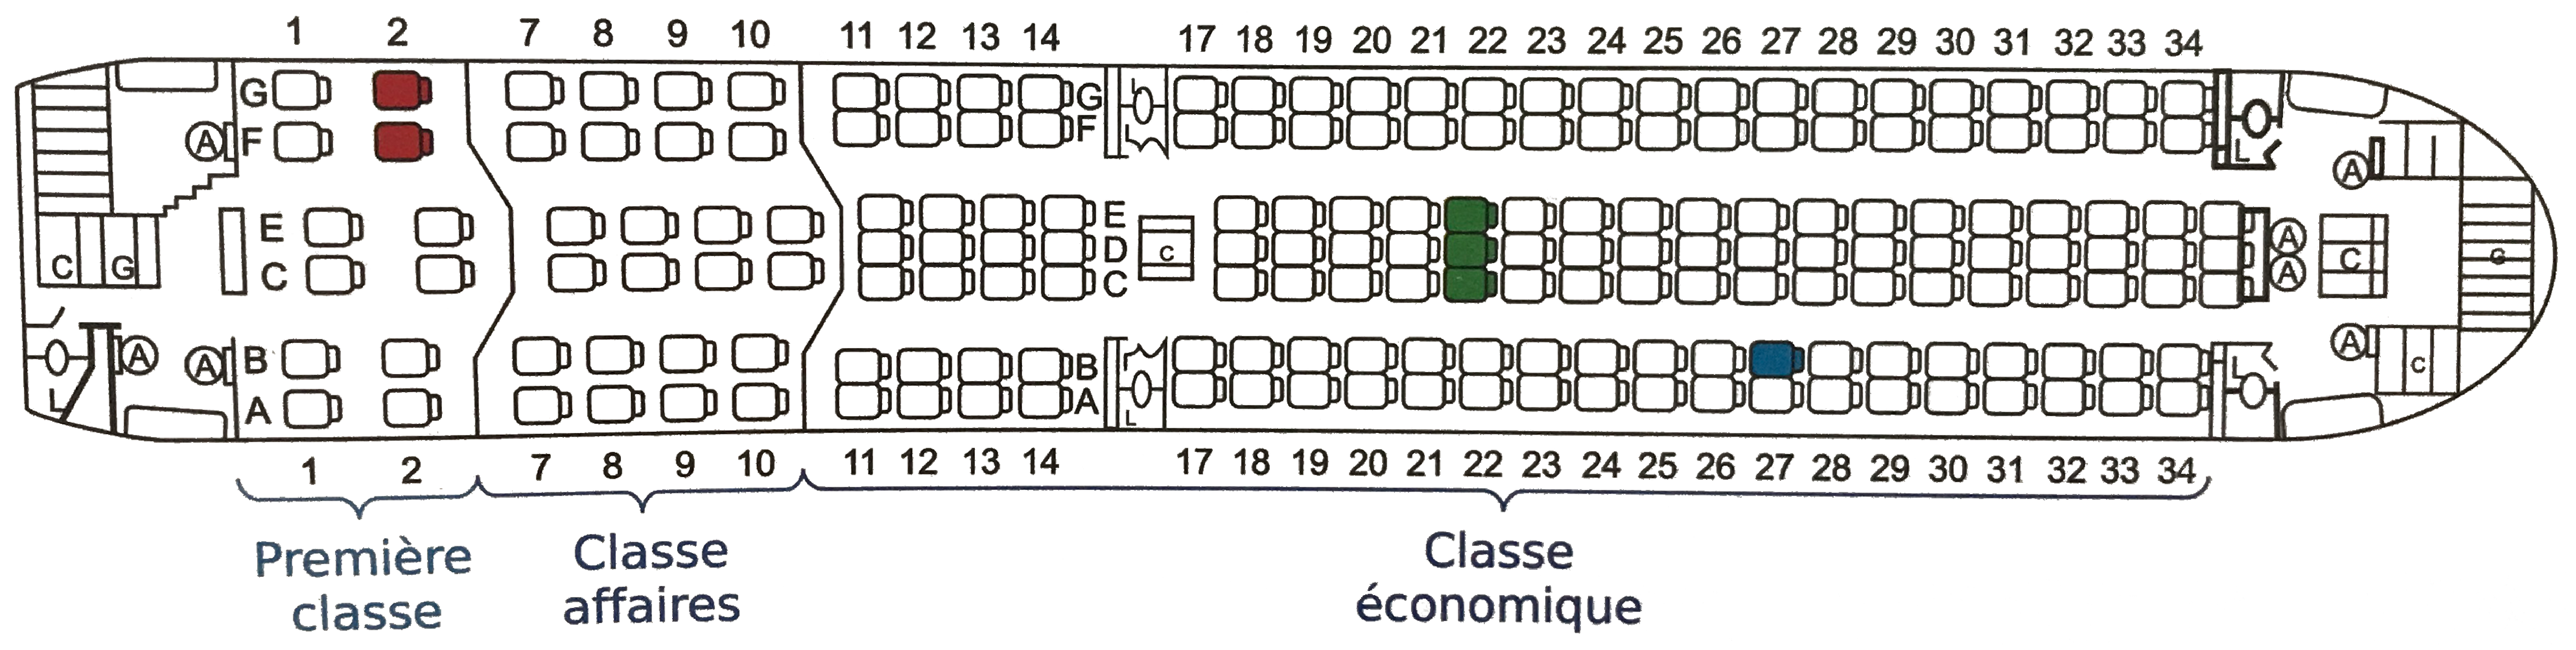
\includegraphics[width=15cm]{boeing}
   \end{center}
   \begin{enumerate}
      \item Indiquer à quelle classe correspond chaque siège : E26 ; E1 ; E7 ; C9 ; B14 ; A34.
      \item Donner la référence des sièges colorés.
      \item Colorier : en rouge les sièges A17 et B17 ; en bleu le siège A1 ; en vert les sièges G29 et F29 ; en noir le siège D12.
   \end{enumerate}
\end{exercice}

\begin{exercice}
   Voici le plan du jardin des plantes de Nantes. \\
  \begin{minipage}{7cm}
      \begin{enumerate}
         \item Combien d'entrées possède ce jardin ?
         \item L'Orangerie se trouve en B1. \\
         Où se trouvent :
         \begin{itemize}
            \item la grande porterie ;
            \item la station de tram ;
            \item la statue Jules Verne ;
            \item la ménagerie ;
            \item le jardin botanique.
         \end{itemize}
         \item Que peut se trouver en :
         \begin{itemize}
            \item C1 ?
            \item D3 ?
            \item C4 ?
            \item B5 ?
         \end{itemize}
         \item Quelles sont les rues qui bordent le jardin des plantes ?
      \end{enumerate}
   \end{minipage}
   \qquad
   \begin{minipage}{9.5cm}
      \includegraphics[width=9.4cm]{jardin}
   \end{minipage}
   \qquad
\end{exercice}

\begin{exercice}
   Voici le plan des trams de l'agglomération de Montpellier : \\ [1mm]
   \begin{minipage}{11.5cm}
      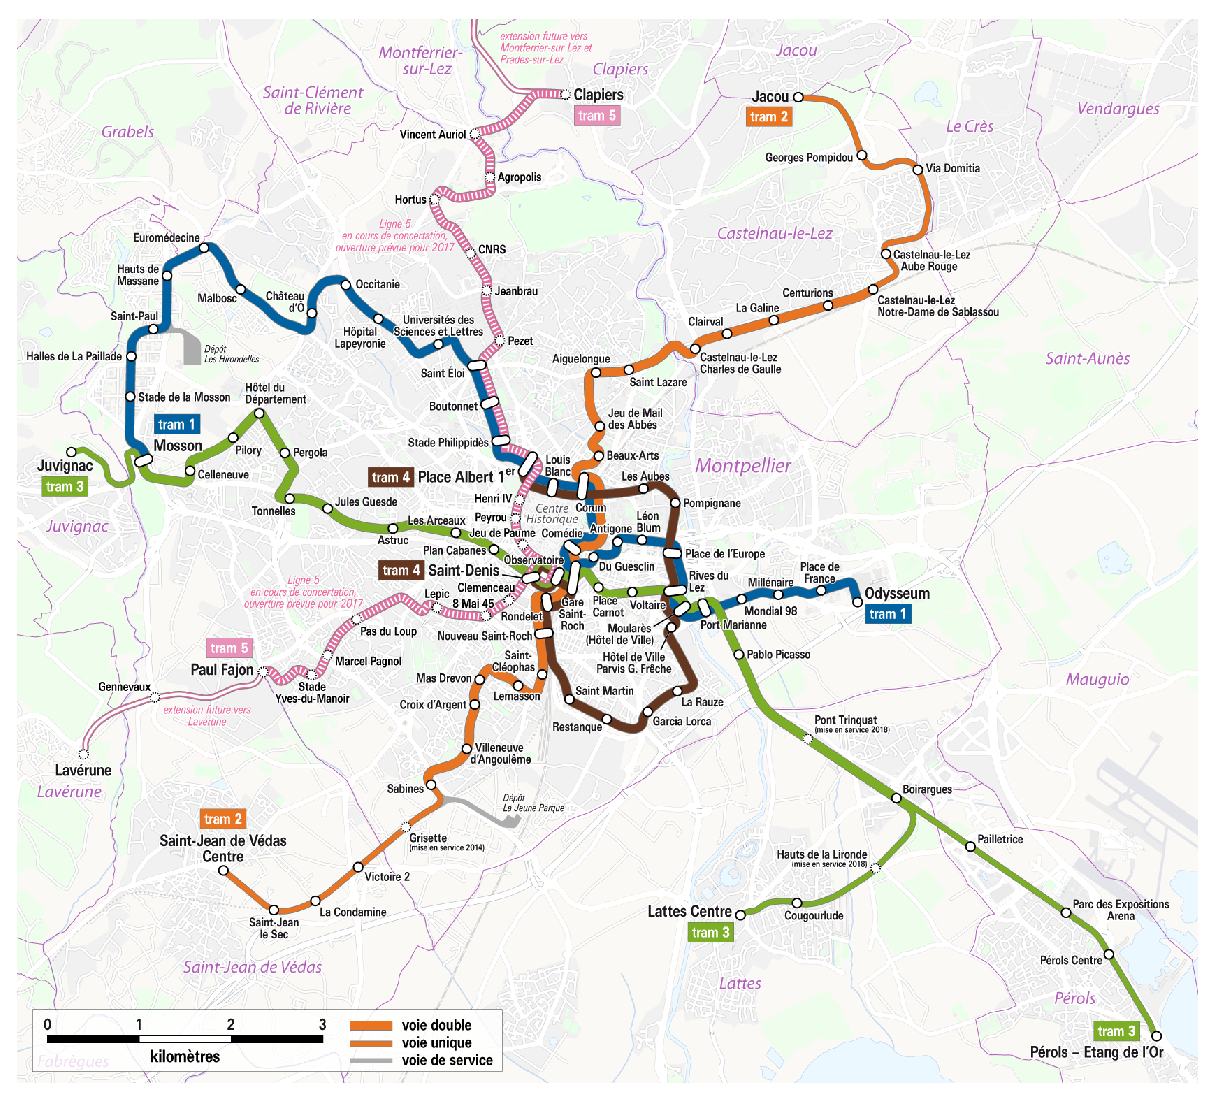
\includegraphics[width=11.5cm]{TAM}
   \end{minipage}
   \quad
   \begin{minipage}{5.5cm}
      \begin{enumerate}
         \item Combien de lignes de tram sont indiquées sur ce plan ?
         \item Combien de lignes de tram sont actuellement en fonctionnement ?
         \item Environ combien de kilomètres mesure la ligne 1 ?
         \item Combien y a-t-il de stations pour la ligne 2 ?
         \item Quelles sont les villes traversées par le ligne 3 ?
         \item Quelle est la particularité de la ligne 4 ?
         \item Quelles sont les deux destinations de la future ligne 5 ?
         \item Quel est l'arrêt le plus proche du collège Simone Veil ?
         \item Vous habitez à Le Crès et souhaitez voir un match de foot au stade de la Mosson. Quel parcours en tram allez-vous effectuer ? 
      \end{enumerate}
   \end{minipage}
\end{exercice}


%%%%%%%%%%%%%%%%%%%%%%%%%%%%%%%%%%%%%%%
%%%%%%%%%%%%%%%%%%%%%%%%%%%%%%%%%%%%%%%
\Recreation

\enigme[La bataille navale]
   \begin{minipage}{5.5cm}  
      \partie[but du jeu.] Faire couler les 5 bateaux de son adversaire.

      \partie[matériel.] Deux grilles composées de 100 cases numérotées horizontalement de 1 à 10 et verticalement de A à J. L'une des grilles sert à disposer ses 5 bateaux et l’autre à marquer les tentatives de localisation des bateaux de l’adversaire. \\  
      {\bf Bateaux à placer} sur la grille :
      \begin{itemize}
         \item 1 porte-avions de 5 cases ;
         \item 1 croiseur de 4 cases ;
         \item 1 contre-torpilleur de 3 cases ;
         \item 1 sous-marin de 3 cases ;
         \item 1 torpilleur de 2 cases.
      \end{itemize}
   
      \partie[règles du jeu.] Les deux joueurs disposent leurs bateaux sur la grille de manière à ce que deux bateaux ne puissent pas être sur des cases adjacentes. \\
      Tour à tour, les joueurs proposent les coordonnées d'un point de la grille en annonçant par exemple \og tir en D8 \fg. L’autre joueur regarde sa grille :
      \begin{itemize}
         \item si un morceau de son bateau s’y trouve, il répond \og touché \fg{} et les deux joueurs marquent cette case d'un cercle ;
         \item si aucun morceau de bateau ne s’y trouve, il répond \og à l'eau \fg{} et les deux joueurs marquent cette case d'une croix ;
         \item si tous les morceaux d’un bateau sont touchés, le joueur dit \og touché-coulé \fg.
      \end{itemize}
      Le premier joueur à couler tous les bateaux de son adversaire gagne.
   \end{minipage}
   \quad
   \begin{minipage}{11cm}
      {\psset{unit=0.95}
      \begin{center}
         \begin{pspicture}(0,0)(11,11)
            \psgrid[gridlabels=0,subgriddiv=0](1,0)(11,10)
            \rput(0.5,0.5){J}
            \rput(0.5,1.5){I}
            \rput(0.5,2.5){H}
            \rput(0.5,3.5){G}
            \rput(0.5,4.5){F}
            \rput(0.5,5.5){E}
            \rput(0.5,6.5){D}
            \rput(0.5,7.5){C}
            \rput(0.5,8.5){B}
            \rput(0.5,9.5){A}
            \rput(0.5,1){\multido{\n=1+1}{10}{\rput(\n,9.5){\n}}}
         \end{pspicture}
      \end{center}
      \begin{center}
         \begin{pspicture}(0,0)(11,11)
            \psgrid[gridlabels=0,subgriddiv=0](1,0)(11,10)
            \rput(0.5,0.5){J}
            \rput(0.5,1.5){I}
            \rput(0.5,2.5){H}
            \rput(0.5,3.5){G}
            \rput(0.5,4.5){F}
            \rput(0.5,5.5){E}
            \rput(0.5,6.5){D}
            \rput(0.5,7.5){C}
            \rput(0.5,8.5){B}
            \rput(0.5,9.5){A}
            \rput(0.5,1){\multido{\n=1+1}{10}{\rput(\n,9.5){\n}}}
         \end{pspicture}
      \end{center}}
   \end{minipage}


\themaM
\graphicspath{{../Ch8_Longueurs_et_perimetre/Images/}}

\chapter{Longueurs et\\périmètres}
\label{C07}

%%%%%%%%%%%%%%%%%%%%%%%%%%%%%%%%%%%%%%%%%%
\begin{prerequis}[Connaissances et compétences abordées]
   \begin{itemize}
      \item Distance entre deux points.
      \item Connaître le lien entre les unités de numération et les unités de mesure (exemple : dixième -> dm, centième -> cm).
      \item Notion de longueur : cas particulier du périmètre.
      \item Comparer des périmètres avec ou sans recours à la mesure (par exemple en utilisant une ficelle, ou en reportant les longueurs des côtés d’un polygone sur un segment de droite avec un compas).
      \item Calculer le périmètre d’un polygone en ajoutant les longueurs de ses côtés.
   \end{itemize}
\end{prerequis}

\vfill

\begin{debat}[Débat : le compas, un instrument de report de mesures]
   Étymologiquement le mot {\bf compas} vient du latin {\it compassare} signifiant - qui partage le même pas, la même mesure - et qui fait donc référence à un instrument qui mesure et non qui trace des cercles.
   \flushright{\it\footnotesize Source : https://compas-passion.jimdo.com}. \\
   \begin{center}
      \small
      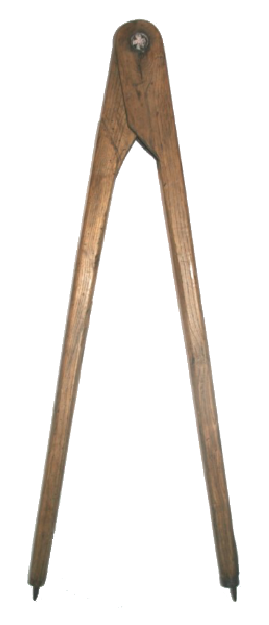
\includegraphics[height=4.5cm]{compas_simple}
      \qquad
      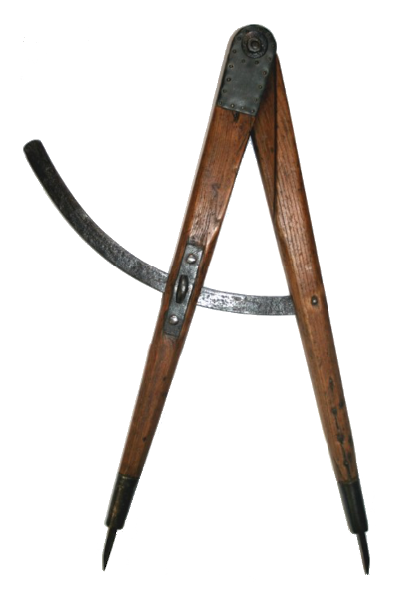
\includegraphics[height=4.5cm]{compas_secteur}
      \qquad
      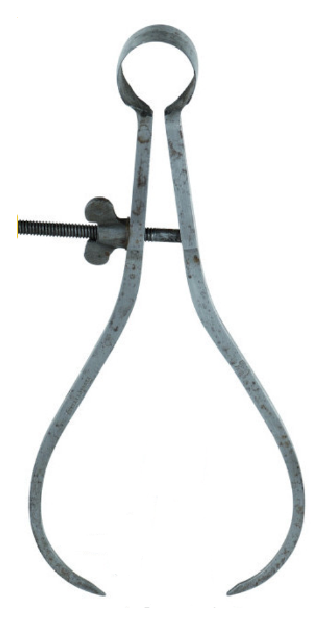
\includegraphics[height=4.5cm]{compas_epaisseur}
      \qquad
      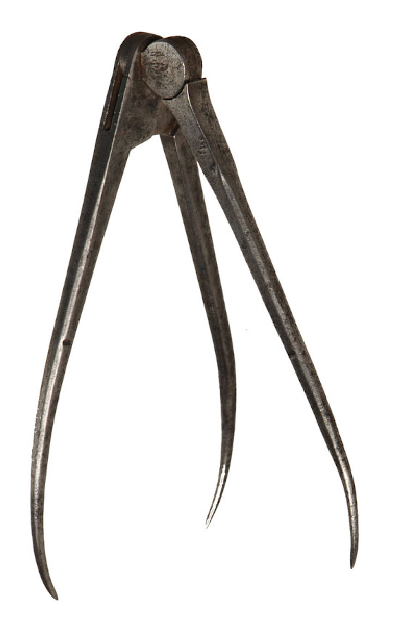
\includegraphics[height=4.5cm]{compas_3jambes} \\
      Compas simple \quad Compas à secteur courbe \; Compas d'épaisseur \quad Compas à trois jambes
   \end{center}
   \bigskip
   \begin{cadre}[B2][F4]
      \begin{center}
         Vidéo : \href{https://www.youtube.com/watch?v=gXOW4e708Hs&vl=fr}{\bf Dessin d'un cercle parfait sans outils}, chaîne YouTube de {\it Rajarts}.      \end{center}
   \end{cadre}
\end{debat}

\vfill

\textcolor{PartieGeometrie}{\large\sffamily\bfseries Cahier de compétences} : chapitre 11, exercices 1 ; 3 ; 4 ; 6 ; 23 ; 24 ; 25 ; 31 ; 37.

%%%%%%%%%%%%%%%%%%%%%%%%%%%%%%%%%%%%
%%%%%%%%%%%%%%%%%%%%%%%%%%%%%%%%%%%%%
\activites

\begin{activite}[L'art de mesurer]
   {\bf Objectifs} : mesurer une longueur et le périmètre d'un polygone avec un étalon et une règle ; comparer des méthodes, communiquer.
   \begin{QCM}
      \partie[mesurer grâce à un étalon]
         On considère la bandelette en bas de page. La découper puis donner en fonction de cette bande la mesure de la longueur d'un stylo, le périmètre du cahier de compétences et le périmètre de votre table. \\
         Écrire les résultats dans le tableau ci-dessous et comparer avec les autres élèves de la classe. \\
         
      \partie[créer une graduation]
         Avec la bandelette entière, il est difficile d'évaluer correctement les mesures demandées. Plier la bande en dix parties égales : une partie correspond donc à un dixième de bandelette. Mesurer de nouveau les trois objets cités en nombre de dixièmes de bandelette. \\
         Écrire les résultats dans le tableau ci-dessous et comparer avec les autres élèves de la classe. \\
      
      \partie[mesurer à l'aide d'une règle graduée]
         Enfin, refaire ces mesures à l'aide d'une règle graduée. \\
         Écrire les résultats dans le tableau ci-dessous et comparer avec les autres élèves de la classe. \\
         Débattre des avantages et inconvénients de chacun des outils. \\
      
      \begin{center}
         {\hautab{1.5}
         \small
         \begin{tabular}{c|C{4}|C{4}|C{4}|}
            \cline{2-4}
            & Longueur du stylo & Périmètre du cahier & Périmètre de la table \\
            \cline{2-4}
            & \begin{pspicture}(0,0.3)(4,4)
                  \pspolygon(1.8,0.5)(2.2,0.5)(2.2,3)(2,3.4)(1.8,3)
                  \psarc(2,3.4){0.06}{-120}{-70}
                  \psline(1.8,3)(1.9,2.9)(2,3)(2.1,2.9)(2.2,3)
                  \psset{linecolor=lightgray}
                  \psline(1.9,0.5)(1.9,2.9)
                  \psline(2,0.5)(2,2.98)
                  \psline(2.1,0.5)(2.1,2.9)
               \end{pspicture}
            & \begin{pspicture}(0,0.3)(4,4)
                  \psframe(1,0.5)(3,3.5)
                  \rput(2,2){\begin{minipage}{1.5cm} \footnotesize Cahier\\de\\compétences \end{minipage}}
                  \rput(2.5,3){\large 6\up{e}}
               \end{pspicture}
               & \begin{pspicture}(0,0.3)(4,4)
                     \psline(0.5,0.7)(0.5,2.5)(1.5,3.3)(3.5,3.3)(2.5,2.5)(2.5,0.7)
                     \psline(3.5,1.7)(3.5,3.3)
                     \psline(0.5,2.5)(2.5,2.5)
                     \psline(0.5,2.3)(2.5,2.3)(3.5,3.1)
                     \psline(1.5,1.7)(1.5,2.3)
                  \end{pspicture} \\
            \hline
            Avec l'étalon & & & \\
            \hline
            Etalon gradué & & & \\
            \hline
            Règle graduée & & & \\
            \hline
         \end{tabular}}
      \end{center}
      \bigskip
   \end{QCM}
   \vfill
   Bandelette à découper :
   \begin{center}
      \begin{pspicture}(0,0)(15,1.5)
         \psframe(0,0)(15,1.5)
     \end{pspicture}
  \end{center}
\end{activite}


%%%%%%%%%%%%%%%%%%%%%%%%%%%%%%%%%%%%%%
%%%%%%%%%%%%%%%%%%%%%%%%%%%%%%%%%%%%%%
\cours 

%%%%%%%%%%%%%%%%%%%%%%%%%%%%%%%%%%%%%%%%%%
\section{Le compas comme instrument de report de mesure}

\begin{methode}[Reporter une longueur au compas]
   Pour reporter la mesure de la longueur d'un segment avec un compas, prendre la longueur de ce segment en plaçant chaque pointe du compas sur l'une des extrémités du segment puis la reporter sur une autre portion de droite.
   \exercice
      Reproduire un segment $[CD]$ de même mesure que $[AB]$. \\
      \begin{pspicture}(0,0.5)(4,1.5)
         \psline[linecolor=violet]{|-|}(1,0.5)(2.8,1.4)
         \rput(1,0.1){\textcolor{violet}{$A$}}
         \rput(2.8,1){\textcolor{violet}{$B$}}
      \end{pspicture}
   \correction
      {\psset{unit=0.7}
      \begin{pspicture}(-3,0)(4.5,3.5)
         \psline[linecolor=violet]{|-|}(1,0.5)(2.8,1.4)
         \rput(1,0.1){\textcolor{violet}{$A$}}
         \rput(2.8,1){\textcolor{violet}{$B$}}
         \compas{2}{0.8}{25}{1}{18}
         \psline[linewidth=1mm]{->}(2,3.9)(4.5,3.7)
      \end{pspicture}
      \begin{pspicture}(0.5,-0.5)(4,3.5)
         \rotatebox{-27}{
            \psline(0,0)(4,2)
            \rput(1,0.1){\textcolor{cyan}{$C$}}
            \rput(2.8,1){\textcolor{cyan}{$D$}}
            \psline[linecolor=cyan]{|-|}(1,0.5)(2.8,1.4)
            \psarc[linecolor=gray!50](2.8,1.4){2}{180}{240}
            \compas{2}{0.8}{25}{1}{18}}
      \end{pspicture}}
\end{methode}




\section{Unités de longueur} %%% 1

On peut mesurer une longueur grâce au mètre (m) et à toutes les unités qui en découlent :
   \begin{center}
   \begin{CLtableau}{0.9\linewidth}{8}{p{3cm}}
      \hline
      Préfixe & kilo & hecto & déca & & déci & centi & milli \\
      \hline
      Signification & 1 000 & 100 & 10 & 1 & 1/10 & 1/100 & 1/1 000 \\
      \hline
      Unité de longueur & km & hm & dam & m & dm & cm & mm \\
      \hline
      Exemple & & $9$ & $7$ & $3$ & $2$ & $1$ & \\
      \hline
   \end{CLtableau}
   \end{center}

\begin{exemple*1}
   $\ukm{0,97321} =\uhm{9,7321} =\udam{97,321} =\um{973,21}=\udm{9732,1} =\ucm{97321} =\umm{973210}$. Pour passer d'une unité à une autre, on multiplie/divise par 10, 100, 1 000 \dots
\end{exemple*1}

\begin{definition}
   La {\bf longueur} $AB$ d'un segment [$AB$] est la distance qui sépare ses deux extrémités $A$ et $B$.
\end{definition}


%%%%%%%%%%%%%%%%%%%%%%%%%%%%%%%%%%%%%
\section{Périmètre d'un polygone}

\begin{definition}
   Le \textbf{périmètre} d'une figure est la mesure du contour de cette figure.
\end{definition}

\begin{propriete}
   Pour calculer le périmètre d'un polygone, on additionne la mesure de chacun de ses segments.
\end{propriete}

\begin{exemple}[0.5]
   {\psset{unit=0.45}
   \begin{pspicture}(-0.5,0)(11,5.5)
      \psgrid[subgriddiv=0,gridlabels=0pt,gridcolor=gray](11,5)
      \put(1,1){\pspolygon[fillstyle=solid,fillcolor=B2,linewidth=0.1](0,0)(2,0)(2,3)(0,3)(0,2)(1,2)(1,1)(0,1)(0,0)}
      \put(4,1){\pspolygon[fillstyle=solid,fillcolor=A2,linewidth=0.1](0,0)(2,0)(2,2)(1,2)(1,3)(0,3)(0,0)}
      \put(7,1){\pspolygon[fillstyle=solid,fillcolor=J2,linewidth=0.1](1,0)(2,0)(2,1)(3,1)(3,2)(2,2)(2,3)(1,3)(1,2)(0,2)(0,1)(1,1)(1,0)}
      \rput(2.5,2.4){\textbf{A}}
      \rput(5,2.4){\textbf{B}}
      \rput(8.5,2.4){\textbf{C}}
      \psline[linewidth=0.4mm]{|-|}(6,4)(7,4)
      \rput(6.5,4.6){\small$u.\ell$.}
   \end{pspicture}}
\correction
   $u.\ell$ désigne l'unité de longueur :
   \begin{itemize}
      \item le périmètre de la figure A vaut 12 $u.\ell$;   
      \item le périmètre de la figure B vaut 10 $u.\ell$;
      \item le périmètre de la figure C vaut 12 $u.\ell$
   \end{itemize} 
\end{exemple}


%%%%%%%%%%%%%%%%%%%%%%%%%%%%%%%%%%%%%%
%%%%%%%%%%%%%%%%%%%%%%%%%%%%%%%%%%%%%%
\exercicesbase

\begin{colonne*exercice}

\serie{Reporter des mesures} %%%%%%%%%%%%%%%%%%%%%%%%%%

\begin{exercice}
   Reporter la mesure de chaque segment qui compose les deux polygones sur une droite. En déduire lequel de ces deux polygones a le plus grand périmètre.
   \begin{pspicture}(0.5,0.5)(8,6.5)
      \pspolygon(1,1)(3,1)(4,5)(2,6)
      \pspolygon(5,1)(7,2)(8,3)(7,4)(5,4)(4,3)
      \rput(2.5,3.2){\large 1}
      \rput(5.9,2.8){\large2}
   \end{pspicture}
\end{exercice}

\begin{exercice}
   À l'aide d'un compas, classer ces segments du plus petit au plus grand. Vérifier ensuite en mesurant chaque segment.
   \begin{center}
   {\psset{unit=0.55}
      \begin{pspicture}(0,0)(13,10)
         \pstGeonode[PointSymbol=+,PosAngle={180,0,-100,80,130,-60,170,-10,-100,80}](1,2){A}(7,2){B}(1,4){C}(2,9){D}(7,8){E}(11,2){F}(3,5){G}(8,4){H}(12,2.5){I}(13,9){J}
         \pstLineAB{A}{B}
         \pstLineAB{C}{D}
         \pstLineAB{E}{F}
         \pstLineAB{G}{H}
         \pstLineAB{I}{J}
      \end{pspicture}}
   \end{center}
\end{exercice}


\serie{Calculer de périmètres} %%%%%%%%%%%%%%%%%%%%

\begin{exercice}
   En prenant comme unité de longueur la longueur du côté d'un carreau du cahier, réaliser trois figures différentes qui ont un périmètre de douze unités.
\end{exercice}

\medskip

\begin{exercice}
   Sachant que l'unité de longueur est la longueur d'un côté de carreau, déterminer le périmètre de chacune des figures suivantes.
   \begin{center}
      \psset{unit=0.52}
      \begin{pspicture}(0,-1.5)(15,10)
         \psgrid[subgriddiv=0,gridlabels=0,gridcolor=lightgray](0,-1)(15,10)
         \psset{linewidth=0.3mm}
         \psframe(1,1)(4,3)
         \rput(2.5,2){\ding{205}} %4
         \pspolygon(5,0)(11,0)(11,1)(10,1)(10,4)(8,4)(8,2)(5,2)
         \rput(8.5,1.5){\ding{206}} %5
         \pspolygon(1,4)(1,9)(5,9)(5,8)(2,8)(2,7)(4,7)(4,6)(2,6)(2,4)
         \rput(1.5,6.5){\ding{202}} %1
         \pspolygon(6,7)(8,7)(8,8)(11,8)(11,9)(6,9)
         \rput(7.5,8.4){\ding{203}} % 2
         \pspolygon(5,4)(5,6)(12,6)(12,8)(14,8)(14,4)(13,4)(13,2)(14,2)(14,1)(12,1)(12,2)(11,2)(11,5)(6,5)(6,5)(6,4)
         \rput(13,5.5){\ding{204}} %3
      \end{pspicture}
   \end{center}
\end{exercice}
         
\begin{exercice}
   Classer ces figures dans l'ordre croissant de leur périmètre \og au jugé \fg{} puis déterminer le périmètre de chaque figure, exprimé en unités de longueur (u.l.) et vérifier que le classement est correct.
   \begin{center}
      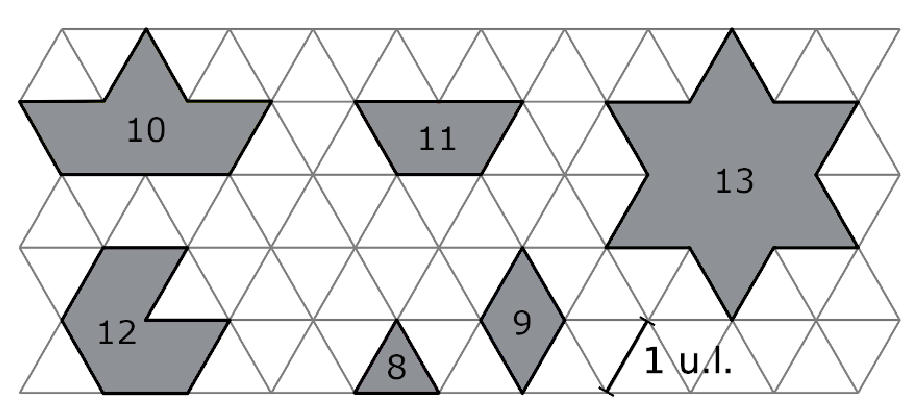
\includegraphics[width=8cm]{triangulaire}
   \end{center}
\end{exercice}

\medskip

\begin{exercice}
   Déterminer le périmètre de chaque figure en \ucm{}. \smallskip
   \begin{center}
      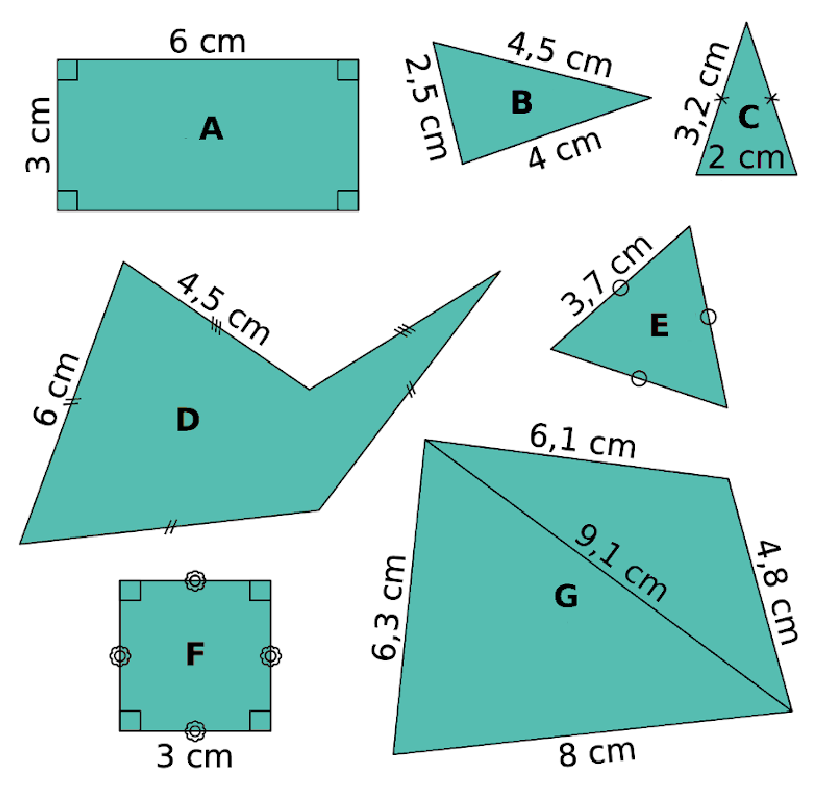
\includegraphics[width=8cm]{perimetres_divers}
   \end{center}
\end{exercice}

\hfill {\footnotesize\it Source : inspiré de Sesamath, le manuel 6\up{e}. Génération 5 - 2013}
\end{colonne*exercice}


%%%%%%%%%%%%%%%%%%%%%%%%%%%%%%%%%%%%%%%
%%%%%%%%%%%%%%%%%%%%%%%%%%%%%%%%%%%%%%%
\Recreation
   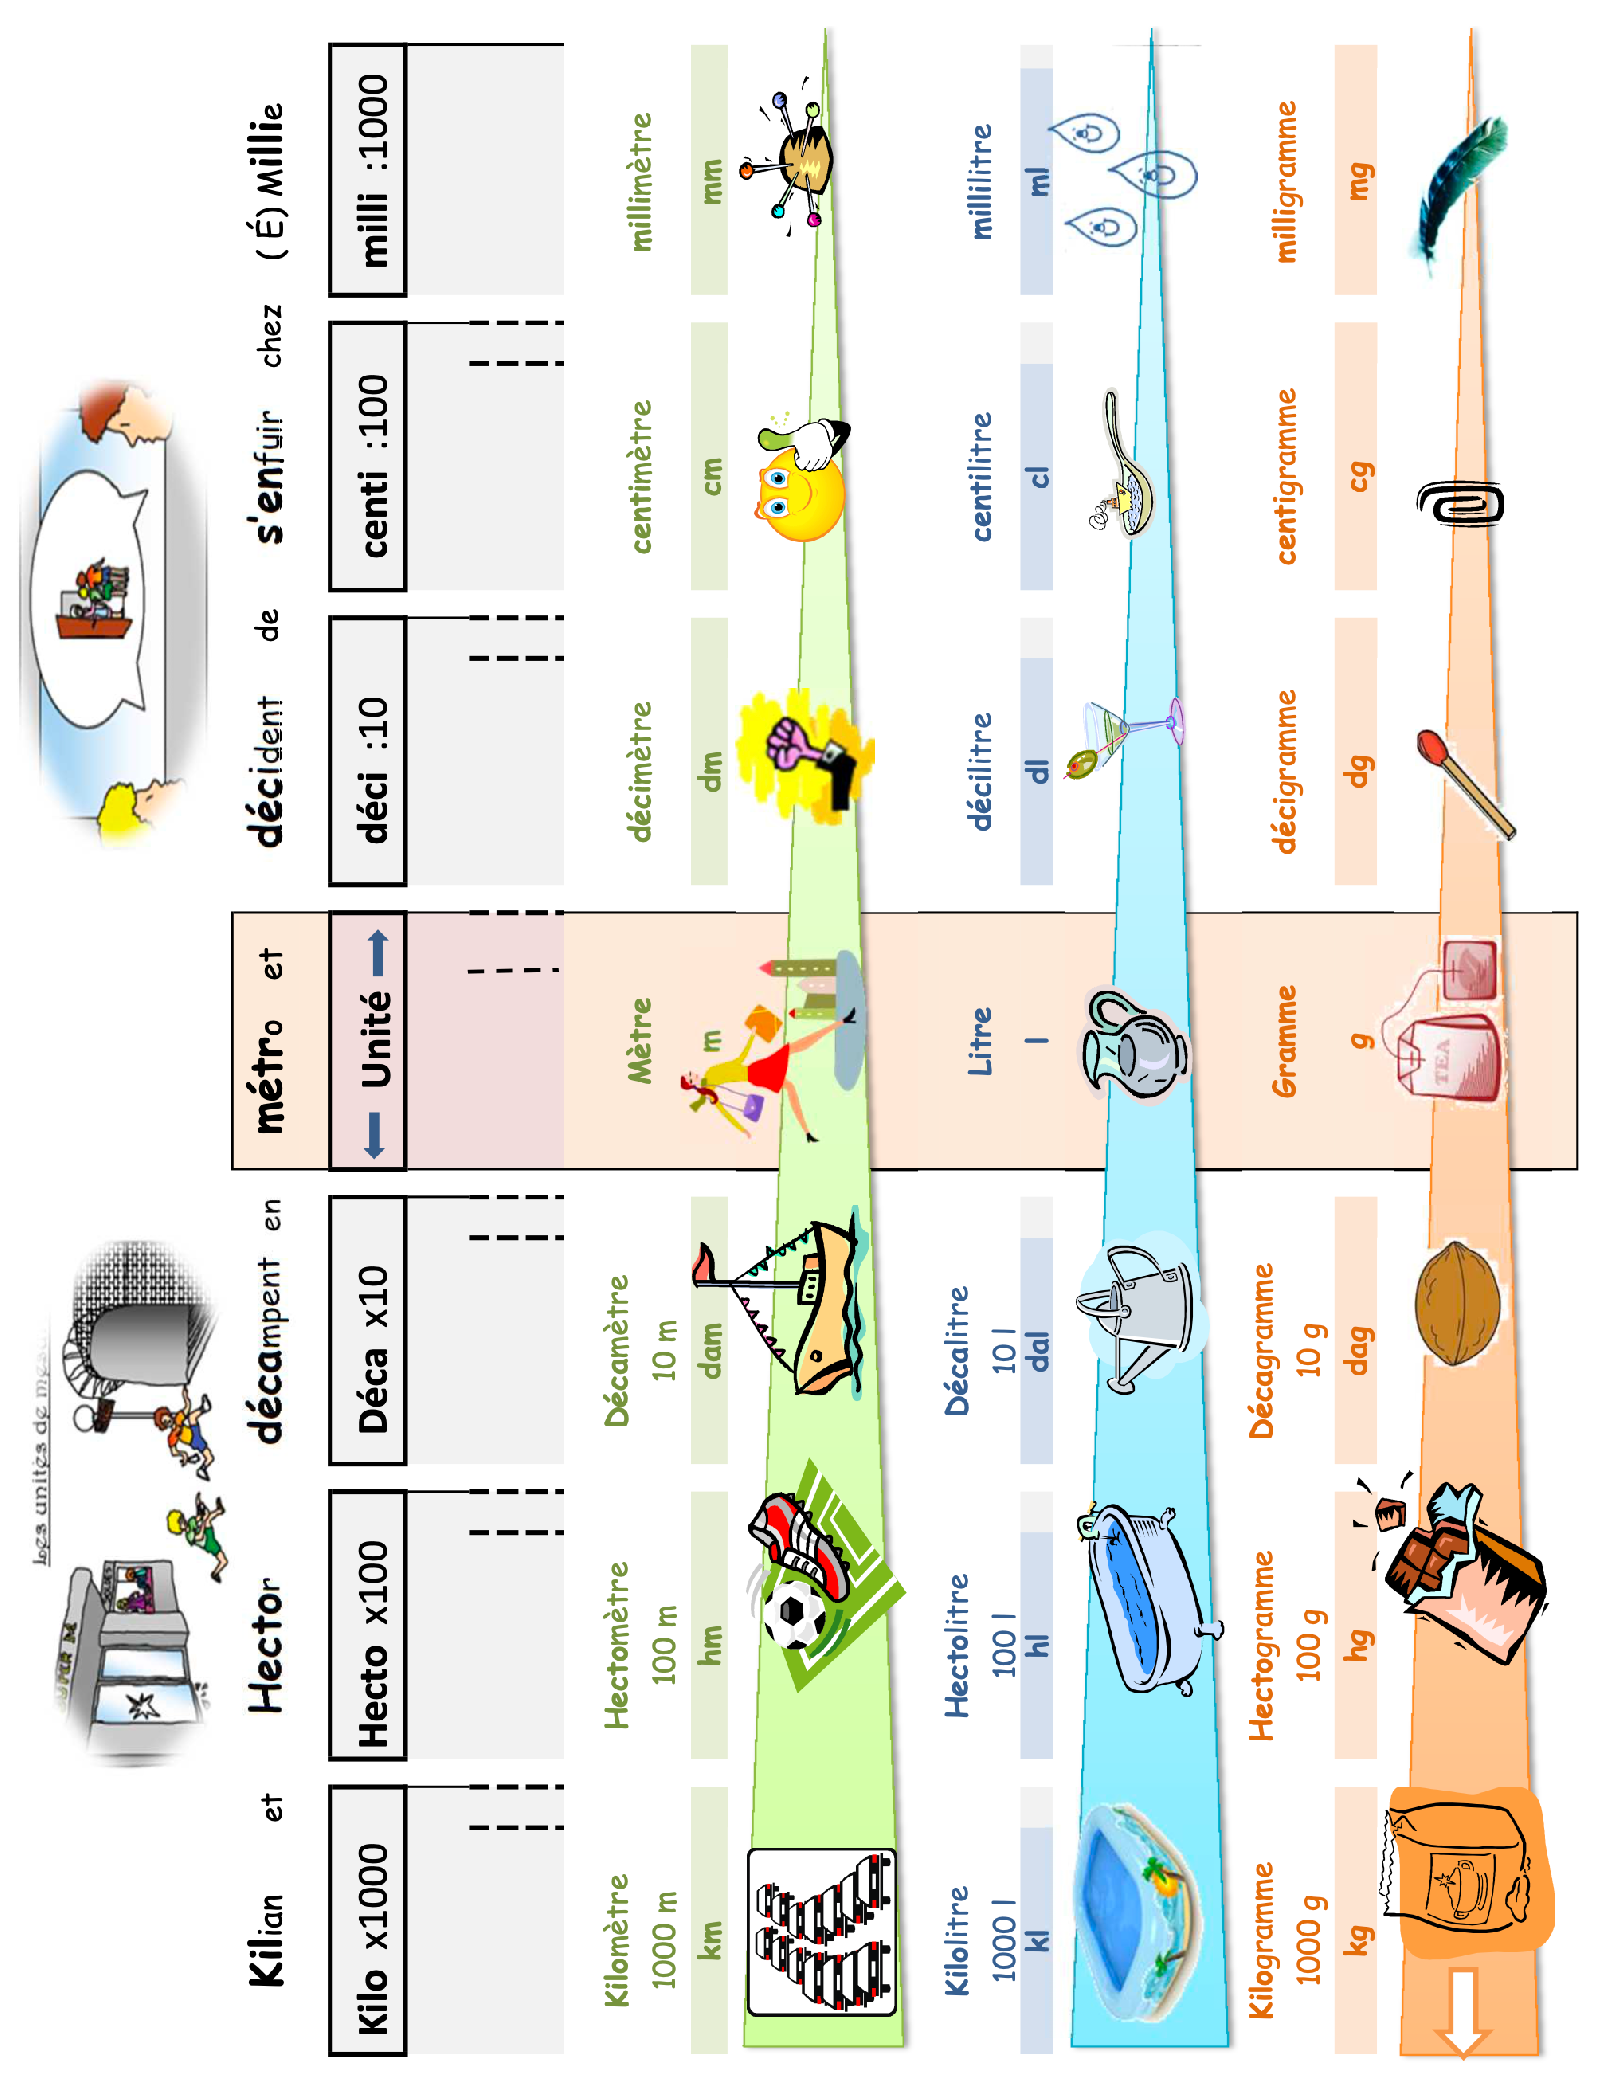
\includegraphics[width=16.6cm]{tableau_mesures}
   \begin{flushright}
      {\it\footnotesize Source : \href{https://ateliersdys.ch/les-unites-de-mesure}{Les ateliers DYS}}
   \end{flushright}


\themaN
\graphicspath{{../Ch12_Additions_et_soustractions/Images/}}

\chapter{Additions et\\soustractions}
\label{C08}


%%%%%%%%%%%%%%%%%%%%%%%%%%%%%%%%%%%%%%%%%%
\begin{prerequis}[Connaissances et compétences abordées]
   \begin{itemize}
      \item Connaître des procédures élémentaires de calcul, notamment : rechercher le complément à l’entier supérieur.
      \item Connaître des propriétés de l’addition, de la soustraction et notamment la commutativité et l'associativité.
      \item Connaître et mettre en œuvre un algorithme de calcul posé pour effectuer l’addition, la soustraction de nombres entiers ou décimaux.
   \end{itemize}
\end{prerequis}

\vfill

\begin{debat}[Débat : levez vos ardoises !] 
   {\bf Claude Martin} (1735-1800) est un soldat français. À sa mort, il lègue une grande partie de sa fortune à la création d'écoles \og La Martinière \fg{} à Lyon, Lucknow et Calcutta. À Lyon, on invente une technique d’utilisation de l’ardoise portant son nom : il s'agit de la méthode \og La Martinière \fg{} dont voici une description tirée du manuel de CM2 de 1969 :
   \begin{itemize}
      \item les enfants ont devant eux leur ardoise et un morceau de craie ;
      \item le maître pose la question et la répète une fois ;
      \item le maître laisse les élèves réfléchir quelques instants ;
      \item au signal (coup de règle), les enfants écrivent la réponse ;
      \item au second coup de règle, les élèves doivent lever l’ardoise ;
      \item le maître contrôle les résultats et on fait la correction. \\ [-15mm]
   \end{itemize}
   \begin{center}
      \begin{pspicture}(0,-0.5)(3.5,3.8)
         \psset{fillstyle=solid}
         \psframe[fillcolor=brown!50,framearc=.1](0,0)(3.5,2.5)
         \psframe[fillcolor=black!90,framearc=.1](0.3,0.3)(3.2,2.2)
         \rput(1.75,1.25){\textcolor{white}{\large $1+1=2$}}
      \end{pspicture}
   \end{center}
   \begin{cadre}[B2][F4]
      \begin{center}
         Vidéo : \href{https://www.dailymotion.com/video/x2j0wh1}{\bf Plickers : une méthode la Martinière \og moderne \fg}, académie d'{\it Orléans Tours}.
      \end{center}
   \end{cadre}
\end{debat}

\vfill

\textcolor{PartieGeometrie}{\large\sffamily\bfseries Cahier de compétences} : chapitre 2, exercices 1 à 14 et 58.


%%%%%%%%%%%%%%%%%%%%%%%%%%%%%%%%%%%%
%%%%%%%%%%%%%%%%%%%%%%%%%%%%%%%%%%%%%
\activites

\begin{activite}[Le labyrinthe]
   {\bf Objectifs :} effectuer une addition ou une soustraction mentalement ; manipuler les nombres entiers et décimaux.

   \begin{QCM}
      \partie[règle du jeu]
         Pour chaque labyrinthe, l'objectif est de trouver le chemin qui mène à la sortie en effectuant l'une des opérations proposées et en passant d'une case à l'autre horizontalement ou verticalement uniquement. \\
         Le point de départ est le nombre entouré dans la première ligne et le point d'arrivée est le nombre entouré dans la dernière ligne. \\
         
      \partie[à vous de jouer !]
         \begin{center}
            {\hautab{2.2}
            \begin{tabular}{|*{5}{C{0.7}|}}
               \multicolumn{5}{c}{$+6$ ou $-6$} \\
               \hline
               28 & \textcircledd{42} & 49 & 21 & 27 \\
               \hline
               32 & 36 & 30 & 24 & 30 \\
              \hline
               60 & 54 & 18 & 42 & 36 \\
               \hline
               66 & 48 & 54 & 48 & 56 \\
               \hline
               \textcircledd{72} & 42 & 30 & 36 & 48 \\
               \hline
            \end{tabular}
            \hspace*{1cm}
            \begin{tabular}{|*{5}{C{0.7}|}}
               \multicolumn{5}{c}{$+9$ ou $-9$} \\
               \hline
               45 & 37 & 29 & \textcircledd{38} & 47 \\
               \hline
               56 & 65 & 56 & 47 & 29 \\
               \hline
               47 & 38 & 65 & 60 & 45 \\
               \hline
               36 & 29 & 20 & 11 & 28 \\
               \hline
               42 & 35 & 42 & \textcircledd{2} & 37 \\
               \hline
            \end{tabular}
            \bigskip

            \begin{tabular}{|*{5}{C{0.7}|}}
               \multicolumn{5}{c}{$+0,5$ ou $-0,5$} \\
               \hline
               5,5 & 5 & \textcircledd{3,5} & 4 & 3,5 \\
               \hline
               6 & 4,5 & 4 & 3,5 & 5,5 \\
               \hline
               5,5 & 7 & 5,5 & 6 & 6,5 \\
               \hline
               5 & 4,5 & 5 & 7,5 & 7 \\
               \hline
               6,5 & \textcircledd{6} & 6,5 & 7 & 2,5 \\
               \hline
            \end{tabular}
            \hspace*{1cm}
            \begin{tabular}{|*{5}{C{0.7}|}}
               \multicolumn{5}{c}{$+0,08$ ou $-0,08$} \\
               \hline
               1,04 & 1,14 & \textcircledd{1,22} & 10,2 & 0,99 \\
               \hline
               0,98 & 1,06 & 1,1 & 0,95 & 0,82 \\
               \hline
               1,06 & 0,98 & 1,07 & 0,9 & 0,86 \\
               \hline
               1,14 & 1,22 & 1,3 & 1,38 & 1,46 \\
               \hline
               0,86 & 0,74 & 0,82 & 0,9 & \textcircledd{1,38} \\
               \hline
            \end{tabular}}
         \end{center}
      \vspace*{1cm}
   \end{QCM}
   
   \begin{flushright}
      {\it\footnotesize Source : inspiré de 123 jeux de nombres, 8 à 13 ans, Accès Édition, 2007.}
   \end{flushright}
\end{activite}


%%%%%%%%%%%%%%%%%%%%%%%%%%%%%%%%%%%%%
%%%%%%%%%%%%%%%%%%%%%%%%%%%%%%%%%%%%%
\cours 

\section{Propriétés des additions et soustractions} %%%%%%%%%%%%

\begin{propriete}
   L'addition est {\bf commutative} (on peut changer l’ordre des facteurs) et {\bf associative} (on peut regrouper les facteurs de la manière dont on veut).
\end{propriete}

\begin{exemple*1}
   $123+234 =234+123 =357$ \\
      $12,3+(0,7+15) =(12,3+0,7)+15 =13+15 =28$.
\end{exemple*1}

\begin{remarque}
   attention, la soustraction n'est pas commutative, par exemple $3-2 \neq2-3$, ni associative, par exemple $(3-2)+1 \neq3-(2+1)$.
\end{remarque}


%%%%%%%%%%%%%%%%%%%%%%%%%%%%%%%%%%
\section{Calcul en ligne et en colonnes}

Pour effectuer une addition ou une soustraction, on peut : calculer mentalement ; calculer en ligne en posant l'opération ; calculer en colonnes en posant l'opération ; calculer grâce à une calculatrice.

\begin{methode}[Priorités opératoires dans un calcul en ligne]
   Dans un calcul comportant des parenthèses, additions et soustractions, on effectue en priorité les calculs dans les parenthèses les plus intérieures, puis les additions/soustractions de gauche à droite. S'il n'y a que des additions, on peut faire les calculs dans l'importe quel {\small ordre}
   \exercice
   Calculer la valeur de $A$ :
   $A =5+3+(15-(9+2))$ \\
   \correction
      $A =5+3+(15-\underline{(9+2)}) =5+3+\underline{(15-\psframebox*[fillcolor=yellow]{11})}$ \\
      $\phantom{A} =\underline{5+3}+\psframebox*[fillcolor=yellow]{4} =\underline{\psframebox*[fillcolor=yellow]{8}+4} =\psframebox*[fillcolor=yellow]{12}$
\end{methode}
 
\begin{propriete}
   Lorsqu'on calcule une somme ou une différence en colonnes, on aligne les chiffres de même rang les uns au-dessus des autres.
\end{propriete}

\begin{exemple}
   Calculer  : \\
   $27,89+1\,298,7$ \\
   $85,8-34,54$.
   \correction
   \opadd[voperation=center,resultstyle=\red,carrystyle=\footnotesize\blue,decimalsepsymbol={,}]{1298,7}{27,89}
   \qquad
   \opsub[voperation=center,resultstyle=\red,carrystyle=\footnotesize\blue,carrysub,lastcarry,columnwidth=2.5ex,offsetcarry=-0.4,decimalsepsymbol={,}]{85,8}{34,54}
   \; ou \;
   \opsub[voperation=center,resultstyle=\red,columnwidth=2.5ex,offsetcarry=-0.4,decimalsepsymbol={,}]{85,8}{34,54} 
   \rput(-0.65,0.7){\textcolor{blue}{/}}
   \rput(-0.65,1.1){\textcolor{blue}{\small 7}}
   \rput(-0.42,0.71){\textcolor{blue}{\small 1}}
\end{exemple}


%%%%%%%%%%%%%%%%%%%%%%%%%%%%%%%%%%%%%%%%
\section{Ordre de grandeur}

\begin{definition}
   Un {\bf ordre de grandeur} d'un nombre est une valeur approchée de ce nombre.
\end{definition}

\begin{exemple*1}
   Ordre de grandeur de $392,5+703,56$ : \\
   une valeur approchée de 392,5 est 400 et une valeur approchée de 703,56 est 700 donc, un ordre de grandeur de $392,5+703,56$ est $400+700 =1\,100$.
\end{exemple*1}


%%%%%%%%%%%%%%%%%%%%%%%%%%%%%%%%%%%%%
%%%%%%%%%%%%%%%%%%%%%%%%%%%%%%%%%%%%%
\exercicesbase

\begin{colonne*exercice}

\serie{Techniques opératoires} %%%%%

\begin{exercice}
   Compléter les égalités suivantes.
   \begin{colenumerate}{2}
      \item $4,5+\pfb =5$
      \item $7,8+\pfb=8$
      \item $0,8+\pfb=1$
      \item $\pfb+0,23=1$
      \item $\pfb+5,8=6$
      \item $\pfb-2,3 =2$
      \item $\pfb-0,9 =4$
      \item $\pfb-5,8 =7$
      \item $7,3-\pfb =7$
      \item \, $8-\pfb =7,6$
   \end{colenumerate}
\end{exercice}

\begin{exercice}
   Donner un ordre de grandeur pour chaque terme puis en déduire un ordre de grandeur du résultat.
   \begin{colenumerate}{2}
      \item $52,758+46,7$
      \item $97,367+4,692$
      \item $149+201+52$
      \item $10,397-4,754$
      \item $49,021-0,003$
      \item $753-148-99$
   \end{colenumerate}
\end{exercice}

\begin{exercice}
   Calculer les sommes en effectuant des regroupements astucieux.
   \begin{enumerate}
      \item $6,5+12,6+1,5$
      \item $36,99+45,74+2,01+13,26$
      \item $9,25+8,7+5,3+16,75$
      \item $7,42+4,2+7,8+25,58$
      \item $3,01+2,9+6,1+7,99$
   \end{enumerate}
\end{exercice}

\begin{exercice}
   Poser et effectuer les opérations suivantes :
   \begin{colenumerate}{2}
      \item $85\,326+40\,383$
      \item $52,21+8,63$
      \item $49,35+7,432+12,7$
      \item $94\,825-732 $
      \item $9,85-2,07$
      \item $83-43,51$
   \end{colenumerate}
\end{exercice}

\medskip

\serie{Écriture des opérations} %%%

\begin{exercice}
   Pour chaque problème, écrire en ligne la (ou les) opération(s) à faire pour le résoudre puis effectuer le calcul à la calculatrice.
   \begin{enumerate}
      \item La somme de deux nombres vaut 78,92. Un des deux nombres est 29,6. Quel est le second nombre ?
      \item La différence de deux nombres est 68,72. Un des deux nombres est 70,35. Quel est le second nombre ?
      \item Philippe fait une randonnée de 13,7 km. Il a parcouru 8,6 km le matin.
Combien lui reste-t-il à parcourir ?
      \item Un manteau coûte 56,80 \euro. Le commerçant me fait une remise de 12,40 \euro. Combien vais-je payer ?
      \item Noé veut acheter un livre. Il a 12,42 \euro{} mais il lui manque 3,45 \euro{}. Quel est le prix du livre ?   
   \end{enumerate}
\end{exercice}


\serie{Défis et problèmes} %%%%%

\begin{exercice}
   Un carré magique est un tableau carré tel que la somme pour chaque ligne, chaque  colonne et chaque diagonale soit la même. Compléter les carrés suivants pour les rendre magiques.
   \begin{center}
      {\hautab{1.8}
      \begin{tabular}{|C{0.5}|C{0.5}|C{0.5}|}
         \hline
         8 & & \\
         \hline
         & 5 & \\
         \hline
         4 & & 2 \\
         \hline
      \end{tabular}
      \qquad
      \begin{tabular}{|C{0.5}|C{0.5}|C{0.5}|}
         \hline
         18 & & 24 \\
         \hline
         & 15 & \\
         \hline
         & & 12 \\
         \hline
      \end{tabular}}
   \end{center}
\end{exercice}

\begin{exercice}
   Compléter les pyramides en suivant la règle suivante : le nombre d’une case est égal à la somme des deux nombres qui se trouvent dans les deux cases qui sont juste en-dessous. \\ [1mm]
   \begin{tikzpicture}
      \pyramidedenombres{4}
      \pyramideplacernombre{1}{1}{32,3}
      \pyramideplacernombre{1}{3}{31,5}
      \pyramideplacernombre{1}{4}{16,8}
      \pyramideplacernombre{2}{1}{63,3}
   \end{tikzpicture}
   \qquad
   \begin{tikzpicture}
      \pyramidedenombres{4}
      \pyramideplacernombre{1}{1}{4,2}
      \pyramideplacernombre{2}{1}{12,5}
      \pyramideplacernombre{3}{1}{21,7}
      \pyramideplacernombre{4}{1}{35}
   \end{tikzpicture}
\end{exercice}

\begin{exercice}
   Le physicien anglais Newton, né en 1642, est mort en 1727. Le mathématicien allemand Gauss, né en 1777, est mort en 1855. La mathématicienne française Sophie Saint Germain est née un an avant Gauss et a vécu trente ans de moins que Newton. En quelle année est-elle décédée ?
\end{exercice}

\begin{exercice}
   Au restaurant avec des amis, Théo se demande si le serveur n'a pas
fait une erreur en calculant l'addition. Voici ce qu'il a sur sa note :
   \begin{center}
      \fbox{\begin{minipage}{5cm}
         3 riz cantonnais \hfill 29,70 \euro \\
        2 poulet-frite \hfill 12, 20 \euro \\
         2 tartes aux pommes \hfill 9,20 \euro \\
         2 glaces à la vanille \hfill 6,40 \euro \\
         TOTAL : \hfill 88, 70 \euro
      \end{minipage}}
   \end{center}
   Calculer un ordre de grandeur de cette addition et dire si le serveur semble avoir fait une erreur.
\end{exercice}

\end{colonne*exercice}


%%%%%%%%%%%%%%%%%%%%%%%%%%%%%%%%%%%%%
%%%%%%%%%%%%%%%%%%%%%%%%%%%%%%%%%%%%%
\Recreation

   \enigme[Addition à l'abaque romain]
      \partie[introduction]
         Pour additionner à l'abaque romain, on inscrit les deux nombres à l'abaque l'un au-dessus de l'autre puis, pour chaque rang, on dénombre les jetons en faisant éventuellement des échanges. \\ [3mm]
         {\bf Exemple :} calcul de $63+52$. Expliquer sous chaque tableau ce qui a été fait dans l'abaque.
         \begin{center}
            \begin{tabular}{C{5}C{5}C{5}}
               \begin{pspicture}(0,0)(3,4)
                  \multido{\n=0+1}{4}{\psline(\n,0)(\n,4)}
                  \multido{\n=3+1}{2}{\psline(0,\n)(3,\n)}
                  \rput(0.5,3.5){C}
                  \rput(1.5,3.5){X}
                  \rput(2.5,3.5){I}
                  \psdots[linecolor=A1](1.3,2.7)(1.7,2.7)(1.3,2.4)(1.7,2.4)(1.3,2.1)(1.7,2.1) %X1
                  \psdots[linecolor=A1](2.3,2.7)(2.5,2.4)(2.7,2.1) %I1
                  \psdots[linecolor=B1](1.3,1.3)(1.7,1.3)(1.5,1)(1.3,0.7)(1.7,0.7) %X2
                  \psdots[linecolor=B1](2.4,1.15)(2.6,0.85) %I2
               \end{pspicture}
               &
               \begin{pspicture}(0,0)(3,4)
                  \multido{\n=0+1}{4}{\psline(\n,0)(\n,4)}
                  \multido{\n=3+1}{2}{\psline(0,\n)(3,\n)}
                  \rput(0.5,3.5){C}
                  \rput(1.5,3.5){X}
                  \rput(2.5,3.5){I}
                  \psdots(1.3,2.7)(1.7,2.7)(1.3,2.4)(1.7,2.4)(1.3,2.1)(1.7,2.1) %X1
                  \psdots(2.3,2.7)(2.5,2.4)(2.7,2.1) %I1
                  \psdots(1.3,1.8)(1.7,1.8)(1.5,1.5)(1.3,1.2)(1.7,1.2) %X2
                  \psdots(2.4,1.65)(2.6,1.35) %I2
                  \pspolygon[linecolor=J1](1.1,1)(1.1,2.9)(1.9,2.9)(1.9,1.5)(1.5,1.3)(1.5,1)
               \end{pspicture}
               &
               \begin{pspicture}(0,0)(3,4)
                  \multido{\n=0+1}{4}{\psline(\n,0)(\n,4)}
                  \multido{\n=3+1}{2}{\psline(0,\n)(3,\n)}
                  \rput(0.5,3.5){C}
                  \rput(1.5,3.5){X}
                 \rput(2.5,3.5){I}
                  \psdot[linecolor=J1](0.5,2.4) %C1
                  \psdots(2.3,2.7)(2.3,2.1)(2.5,2.4)(2.7,2.1)(2.7,2.7) %I1
               \end{pspicture} \\ [3mm]
              \pfb & \pf & \pf \\ [3mm]
              \pfb & \pf & \pf \\ [3mm]
              \pfb & \pf & \pf \\ [3mm]
            \end{tabular}
        \end{center}
      
      \partie[à vous de jouer]
         Effectuer à l'abaque les additions suivantes (représenter dans les tableaux le calcul effectué).
         \begin{center}
            \begin{tabular}{C{3}C{3}C{4}C{5}}
               \begin{pspicture}(0,-1)(3,4)
                  \multido{\n=0+1}{4}{\psline(\n,-1)(\n,4)}
                  \multido{\n=3+1}{2}{\psline(0,\n)(3,\n)}
                  \rput(0.5,3.5){C}
                  \rput(1.5,3.5){X}
                  \rput(2.5,3.5){I}
               \end{pspicture}
               &
               \begin{pspicture}(0,-1)(3,4)
                  \multido{\n=0+1}{4}{\psline(\n,-1)(\n,4)}
                  \multido{\n=3+1}{2}{\psline(0,\n)(3,\n)}
                  \rput(0.5,3.5){C}
                  \rput(1.5,3.5){X}
                  \rput(2.5,3.5){I}
               \end{pspicture}
               &
               \begin{pspicture}(0,-1)(4,4)
                  \multido{\n=0+1}{5}{\psline(\n,-1)(\n,4)}
                  \multido{\n=3+1}{2}{\psline(0,\n)(4,\n)}
                  \rput(0.5,3.5){X}
                  \rput(1.5,3.5){I}
                  \rput(2.5,3.5){$\frac{1}{10}$}
                  \rput(3.5,3.5){$\frac{1}{100}$}
               \end{pspicture}
               &
               \begin{pspicture}(0,-1)(5,4)
                  \multido{\n=0+1}{6}{\psline(\n,-1)(\n,4)}
                  \multido{\n=3+1}{2}{\psline(0,\n)(5,\n)}
                  \rput(0.5,3.5){X}
                  \rput(1.5,3.5){I}
                  \rput(2.5,3.5){$\frac{1}{10}$}
                  \rput(3.5,3.5){$\frac{1}{100}$}
                  \rput(4.5,3.5){$\frac{1}{1000}$}
               \end{pspicture} \\ [1mm]
               $136+321$ & $89+23$ & $23,45+1,3$ & $34,891+59,129$ \\
               = \pf & = \pf & = \pf & = \pf \\ [5mm]
            \end{tabular}
         \end{center}
      
      \partie[le défi de la soustraction]
         Obélix souhaite acheter un sanglier à 234 sesterces. Il dispose d'un menhir à 1622 sesterces. Imaginer une méthode permettant de trouver le résultat sur l'abaque. \\
         Et s'il voulait acheter un deuxième sanglier ?
         


\themaG
\graphicspath{{../Ch19_Les_triangles/Images/}}

\chapter{Les triangles}
\label{C09}


%%%%%%%%%%%%%%%%%%%%%%%%%%%%%%%%
%%%%%%%%%%%%%%%%%%%%%%%%%%%%%%%%
\begin{prerequis}[Connaissances et compétences abordées]
   \begin{itemize}
      \item Reconnaître, nommer, décrire des triangles, dont les triangles particuliers (triangle rectangle, triangle isocèle, triangle équilatéral).
      \item Vocabulaire associé à ces objets et à leurs propriétés : côté, sommet, angle, hauteur.
   \end{itemize}
\end{prerequis}

\vfill

\begin{debat}[Débat : vocabulaire du triangle] 
   Le mot {\bf triangle} est construit à partir du préfixe \og tri \fg, trois et angle, c'est donc un polygone à trois\dots{} angles ! À la renaissance, on hésite entre triangle et trigone (du grec trigônum). Les mathématiciens choisissent {\it triangle} et les astrologues {\it trigone}, qui donnera le mot {\it trigonométrie}, branche des mathématiques qui traite des relations entre distances et angles dans les triangles.
   \begin{center}
      \begin{pspicture}(0,-0.5)(4.3,4.2)
         \pspolygon[fillstyle=solid,fillcolor=A2](0,1.6)(4,0)(4.2,3.8)
         \rput[r](-0.3,1.6){Floride}
         \rput[l](4.4,4){Bermudes}
         \rput[l](4.3,0){Porto Rico}
      \end{pspicture}
   \end{center}
   \begin{cadre}[B2][F4]
      \begin{center}
         Vidéo : \href{https://www.youtube.com/watch?v=MUr7dgn8wdo}{\bf Le triangle des Bermudes}, chaîne YouTube {\it SYMPA}.
      \end{center}
   \end{cadre}
\end{debat}

\vfill

\textcolor{PartieGeometrie}{\large\sffamily\bfseries Cahier de compétences} : chapitre 10, exercices 1 à 5. 


%%%%%%%%%%%%%%%%%%%%%%%%%%%%%%%%%%%%
%%%%%%%%%%%%%%%%%%%%%%%%%%%%%%%%%%%%%
\activites

\begin{activite}[Avec des allumettes]
   {\bf Objectifs} : construire puis nommer des triangles. 
   \begin{QCM}
      Devant vous, vous avez douze allumettes. Pour chacune des questions suivantes, faire la construction si elle est possible avec des allumettes puis faire un dessin pour schématiser la situation. \\
      \begin{enumerate}
         \item Aligner cinq allumettes en les plaçant les unes à côté des autres.
         \smallskip
         \begin{center}
            
\includegraphics[width=2.5cm]{allumette}
\includegraphics[width=2.5cm]{/allumette}
\includegraphics[width=2.5cm]{allumette}
\includegraphics[width=2.5cm]{allumette}
\includegraphics[width=2.5cm]{allumette}
         \end{center}
         \smallskip
         À partir de ce segment de longueur cinq allumettes et en utilisant les douze allumettes, combien peut-on construire de triangles différents ? Ces triangles sont-ils particuliers ? \\ [4cm]
         \item Mêmes questions si l'on place quatre allumettes côte à côte. \\ [3cm]
         \item Mêmes questions si l'on place six allumettes côte à côte. \\ [3cm]
         \item Mêmes questions si l'on place sept allumettes côte à côte ou plus. \\ [3cm]
      \end{enumerate}
   \end{QCM}
\end{activite}


%%%%%%%%%%%%%%%%%%%%%%%%%%%%%%%%
%%%%%%%%%%%%%%%%%%%%%%%%%%%%%%%%
\cours 

\section{Triangles particuliers} %%%%%%%%%

\begin{pspicture}(-5,-0.5)(10,2.5)
   \rput[l](-4,2){Triangle : }
   \rput[l](-4,1.5){$\bullet$ 3 angles}
   \rput[l](-4,1){$\bullet$ 3 côtés}
   \rput[l](-4,0.5){$\bullet$ 3 sommets}
   \rput[l](-4,0){$\bullet$ 3 hauteurs}
   \pstTriangle[PointSymbol=none,linecolor=A1](0,0){U}(4,0){I}(-1,2){O}
   \pstTriangle[PointSymbol=none,linecolor=A1](6,0){Y}(10,0){S}(7,2){E}
   \rput(2,2){\textcolor{A1}{côté}}
   \psline[linecolor=A1]{->}(1.5,1.8)(1.2,1.2)
   \rput(9,2){sommet}
   \psline{->}(8.2,2)(7.3,2)
   \pstMarkAngle[linecolor=J1,MarkAngleType=double,MarkAngleRadius=1,LabelSep=1.8]{O}{I}{U}{\textcolor{J1}{angle}}
   \psset{linecolor=B1}
   \psline(-1,0)(-1,2)
   \psline(-1,0.25)(-0.75,0.25)(-0.75,0)
   \psline(7,0)(7,2)
   \psframe(7,0)(7.25,0.25)
   \rput(5,1.5){\textcolor{B1}{hauteur}}
   \psline{->}(5.8,1.3)(6.8,1)
\end{pspicture}

\begin{definition}
   \begin{itemize}
      \item Un \textbf{triangle rectangle} est un triangle ayant un angle droit.
      \item Un \textbf{triangle isocèle} est un triangle ayant deux côtés de même longueur.
      \item Un triangle \textbf{équilatéral} est un triangle dont tous les côtés sont de même longueur.
   \end{itemize}
\end{definition}


{\psset{unit=0.9}
\begin{pspicture}(-2,-0.8)(4,2.8)
   \pstTriangle[PointSymbol=none](0,0){E}(4,0){C}(0,2){R}
   \pstRightAngle[linecolor=B1]{R}{E}{C}
   \rput(2,-0.5){triangle rectangle}
\end{pspicture}
\begin{pspicture}(-1.5,0.5)(5.5,3.3)
   \pstTriangle[PointSymbol=none](0,1){I}(4,1){O}(2,3){S}
   \pstSegmentMark[SegmentSymbol=MarkHashh,MarkAngle=90,linecolor=A1]{I}{S} 
   \pstSegmentMark[SegmentSymbol=MarkHashh,MarkAngle=90,linecolor=A1]{S}{O}
   \pstLineAB{I}{O}
   \pstMarkAngle[linecolor=J1,MarkAngleType=double]{S}{O}{I}{}
   \pstMarkAngle[linecolor=J1,MarkAngleType=double]{O}{I}{S}{}
   \rput(2,0.5){triangle isocèle}
\end{pspicture}
\begin{pspicture}(0,-0.5)(5,3.3)
   \pstTriangle[PointSymbol=none](0,0){E}(3,0){I}(1.5,2.55){Q}
   \psset{SegmentSymbol=MarkHash,MarkAngle=90,linecolor=A1}
   \pstSegmentMark{E}{Q} 
   \pstSegmentMark{I}{Q}
   \pstSegmentMark{I}{E}
   \psset{linecolor=A1}
   \pstMarkAngle[linecolor=J1]{Q}{I}{E}{}
   \pstMarkAngle[linecolor=J1]{I}{E}{Q}{}
   \pstMarkAngle[linecolor=J1]{E}{Q}{I}{}
   \rput(1.5,-0.5){triangle équilatéral}
\end{pspicture}}

\begin{remarques}
   un triangle équilatéral et un triangle isocèle particulier et un triangle rectangle peut être isocèle, mais pas équilatéral.
\end{remarques}


%%%%%%%%%%%%%%%%%%%%%%%%%%%%%%%%%%
\section{Construction d'un triangle connaissant trois longueurs}

\begin{methode*1}
   Pour construire un triangle $ABC$ dont on connaît les longueurs des trois côtés :
   \begin{itemize}
      \item on trace à la règle graduée l'un des côtés (en général le plus grand), par exemple $[AB]$ ;
      \item on trace un arc de cercle de centre $A$ et de rayon $AC$ ;
      \item on trace un arc de cercle de centre $B$ et de rayon $BC$ ;
      \item le point $C$ se situe à l'intersection des deux arcs de cercle.
   \end{itemize}
   \exercice
   Tracer le triangle $ABC$ tel que : $AB =\ucm{3,5}$ ; $BC =\ucm{2,2}$ et $CA =\ucm{3,2}$.
   %\correction
   \small
   \psset{unit=0.7}
   \begin{pspicture}(-1.5,-1.5)(4.8,3.5)
      \pstGeonode[PointSymbol=none,PosAngle={225,-45}](0,0){A}(3.5,0){B}
      \pstLineAB{A}{B}
      \rput(1.75,-0.25){3,5 cm}
   \end{pspicture}
   \begin{pspicture}(0,-1.5)(4.8,3.5)
      \pstGeonode[PointSymbol=none,PosAngle={225,-45}](0,0){A}(3.5,0){B}
      \pstLineAB{A}{B}
      \psset{linecolor=A1}
      \psarc(0,0){3.2}{30}{60}
      \rput{55}(0.8,1.3){\textcolor{A1}{3,2 cm}}
      \compas{1.5}{1.2}{55}{0.9}{34.5}
      \end{pspicture}
   \begin{pspicture}(0,-1.5)(4.8,3.5)
      \pstGeonode[PointSymbol=none,PosAngle={225,-45}](0,0){A}(3.5,0){B}
      \pstLineAB{A}{B}
      \psset{linecolor=A1}
      \psarc(0,0){3.2}{30}{60}
      \psset{linecolor=B1}
      \psarc[fillstyle=none](3.5,0){2.2}{90}{130}
      \rput{-45}(2.8,0.8){\textcolor{B1}{2,2 cm}}
      \compas{3.3}{1.1}{130}{0.9}{23}
   \end{pspicture}
   \begin{pspicture}(0,-1.5)(2,3.5)
      \pstGeonode[CurveType=polygon,PointSymbol=none,PosAngle={225,90,-45}](0,0){A}(2.5,2){C}(3.5,0){B}
   \end{pspicture}
\end{methode*1}

\begin{remarque}
   on a deux choix de construction pour $C$, d'un côté ou de l'autre du segment.
\end{remarque}


%%%%%%%%%%%%%%%%%%%%%%%%%%%%%%%%%%%
\exercicesbase

\begin{colonne*exercice}

\serie{Reconnaître des triangles} %%%%%%%%%%

\begin{exercice}
   Classer les triangles suivants dans le tableau.
   \begin{center}
      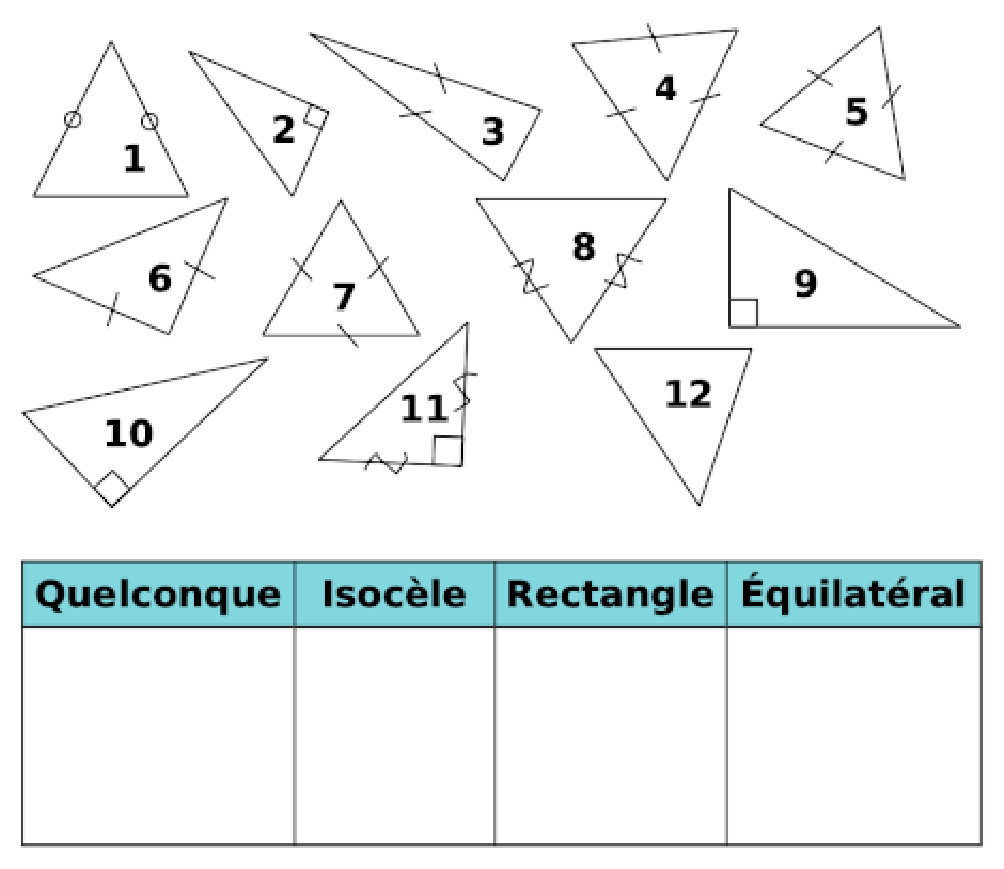
\includegraphics[width=8cm]{classement}
   \end{center}
\end{exercice}

\begin{exercice}
   On considère la figure suivante :
   \begin{center}
     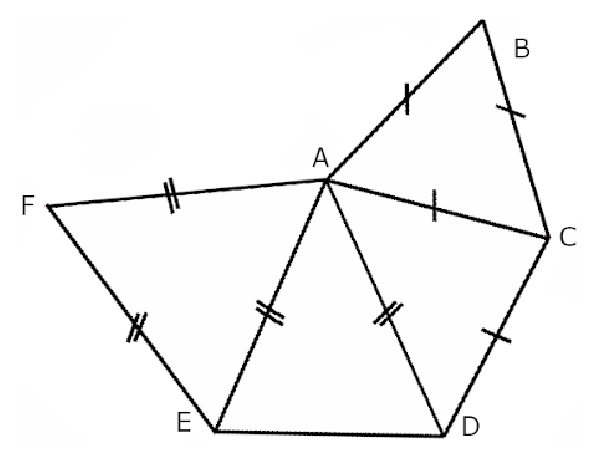
\includegraphics[width=4cm]{triangles}
   \end{center}
   \begin{enumerate}
      \item Nommer les triangles isocèles. Préciser, pour chacun, son sommet principal et sa base.
      \item Nommer les triangles équilatéraux tracés.
      \item Nommer les triangles isocèles que l'on peut tracer en joignant des sommets de la figure.
   \end{enumerate}
\end{exercice}

\serie{Construire des triangles} %%%%%%%%%%%

\begin{exercice}
   Un segment $[AB]$ mesure 7 cm. Construire sur la même figure, lorsque cela est possible, des points $M, N, P, Q$ et $R$ du même côté de $(AB)$, vérifiant les conditions ci-dessous.
   \begin{enumerate}
      \item $AM = 6$ cm et $BM = 4,5$ cm.
      \item $AN=4,8$ cm et $BN=2,2$ cm.
      \item $AP = 5$ cm et $BP = 12$ cm.
      \item $AQ=3,1$ cm et $BQ=3$ cm.
      \item $AR=11$ cm et $BR=4$ cm.
   \end{enumerate}
\end{exercice}

\begin{exercice}
   Tracer chacun des triangles suivants :
   \begin{enumerate}
      \item Le triangle $ABC$ tel que $AB =7$ cm ; $BC = 5$ cm et $CA =$ 6 cm.
      \item Le triangle $GHI$ tel que $HI = 5,1$ cm ; $GI = 5,6$ cm et $GH = 6,3$ cm.
      \item Le triangle équilatéral $EQU$ de périmètre 9 cm.
      \item Le triangle $RST$ isocèle en $S$ de périmètre 13 cm et tel que $ST=4$ cm.
      \item Le triangle $WHY$ rectangle en $W$ tel que \\ $WH =2,5$ cm et $WY =4$ cm.
   \end{enumerate}
\end{exercice}

\medskip

\begin{exercice}
   Voici les trois étapes de construction d'une figure.
   \begin{center}
      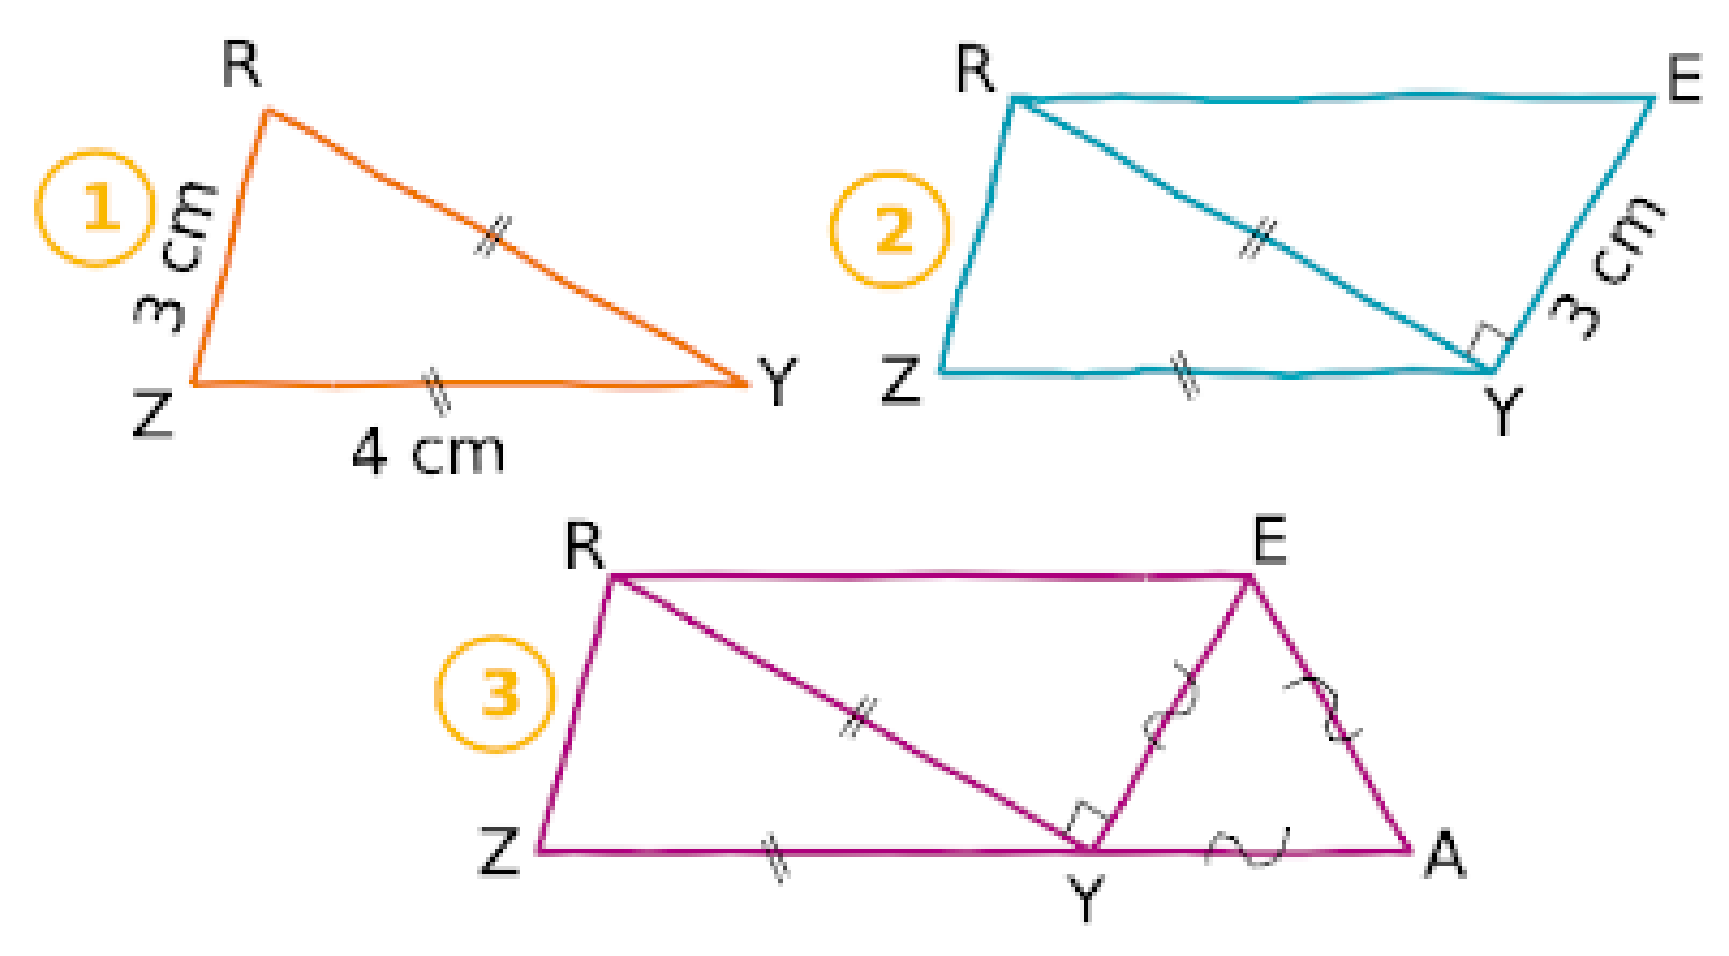
\includegraphics[width=7cm]{programme}
   \end{center}
   \vspace*{-6mm}
   \begin{enumerate}
      \item Écrire un programme permettant de construire la figure.
      \item Construire cette figure taille réelle.
   \end{enumerate}
\end{exercice}

\begin{exercice}
   Remettre les consignes du programme de construction dans l'ordre.
   \begin{center}
      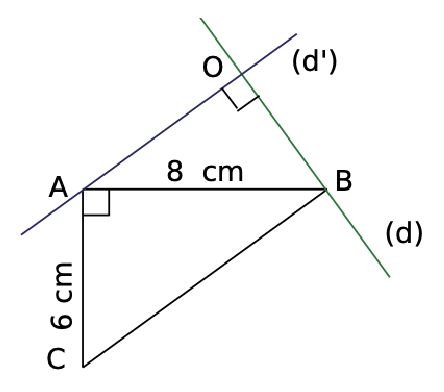
\includegraphics[width=4cm]{consignes}
   \end{center}
   \vspace*{-5mm}
   \begin{itemize}
      \item Trace la droite $(d')$ parallèle à la droite $(BC)$ passant par le point A.
      \item Nomme $O$ le point d'intersection des droites $(d)$ et $(d')$.
      \item Trace un triangle $ABC$ rectangle en $A$ tel que : \\
       $AB = 8$ cm et $AC = 6$ cm.
      \item Trace la droite $(d)$ perpendiculaire à la droite $(d')$ passant par $B$.
   \end{itemize}
\end{exercice}

\hfill {\it\footnotesize Source : Sesamath, le manuel 6\up{e}. Génération 5 - 2013}

\end{colonne*exercice}


%%%%%%%%%%%%%%%%%%%%%%%%%%%%%%%%%%%%%
%%%%%%%%%%%%%%%%%%%%%%%%%%%%%%%%%%%%%
\Recreation

   \enigme[Le triangle de Sierpinski]
     
   \partie[tracé du triangle]
       \begin{enumerate}
          \item Étape 1. Sur une feuille unie, tracer un triangle équilatéral de 16 cm de côté.
          \item Étape 2. 
          \begin{enumerate}
             \item Placer le milieu de chacun des trois côtés du triangle.
             \item Tracer le triangle équilatéral passant par les milieux des trois côtés à l'intérieur du grand triangle.
         \end{enumerate}
         \item Étape 3.
         \begin{enumerate}
            \item Pour les trois triangles situés aux sommets du triangle principal, placer les milieux des côtés.
            \item Construire les trois triangles à l'intérieur.
         \end{enumerate}
         \item Étape 4. Reproduire l'étape 3 pour chacun des neuf triangles ainsi construits.
         \item Décorer/colorier les triangles à votre guise.
     \end{enumerate}
     
      \begin{pspicture}(0.5,0)(4.5,4)
         \pspolygon(0,0)(4,0)(2,3.46)
      \end{pspicture}
      \multido{\i=1+1}{3}
         {\begin{pspicture}(4.5,4)
             \psSier(0,0){4cm}{\i}
          \end{pspicture}} \\
      \hspace*{0.9cm} Étape 1 \hspace*{3.3cm} Étape 2 \hspace*{3.3cm} Étape 3 \hspace*{3.3cm} Étape 4 \\
      
  \partie[dénombrement]
    \begin{enumerate}
       \item En se référant aux dessins ci-dessus, combien y a-t-il de triangles coloriés en noir à chaque étape ? \\ [2mm]
         Étape 1 : \dotfill Étape 2 : \dotfill Étape 3 : \dotfill Étape 4 : \dotfill \medskip
      \item Combien y aurait-il de triangles coloriés en noir à l'étape 5 ? \dotfill À l'étape 6 ? \dotfill
    \end{enumerate}
    
      \vfill

      \begin{center}
         \fbox{
            \begin{minipage}{13cm}
               {\bf Wacław Franciszek Sierpiński} (1882-1969) est un mathématicien polonais. \\
               Il s'intéresse entre autre aux fractales (une fractale est une forme géométrique qui se répète à l'identique lorsqu'on zoome ou qu'on \og dezoome\fg) dont certaines portent son nom : le triangle de Sierpiński, le tapis de Sierpiński et la courbe de Sierpiński. \\
               \begin{pspicture}(-0.7,0)(3,3.5)
                  \psSier(0,0){3cm}{5}
               \end{pspicture}
               \qquad
               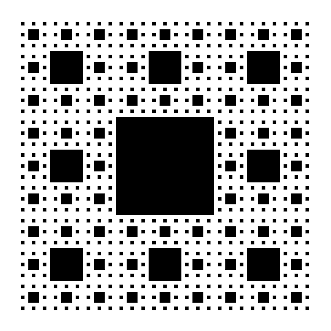
\includegraphics[width=3cm]{Sierpinski_carpet}
               \quad
               \begin{pspicture}(-2,-1.5)(2,1.5)
                  \psSier[unit=0.1,n=4,fillstyle=solid,fillcolor=black] 
               \end{pspicture}
               \medskip
            \end{minipage}}
      \end{center}



\themaM
\graphicspath{{../Ch18_Aires_et_surfaces/Images/}}

\chapter{Aires par pavages}
\label{C10}


%%%%%%%%%%%%%%%%%%%%%%%%%%%%%%%%%%%%%
%%%%%%%%%%%%%%%%%%%%%%%%%%%%%%%%%%%%%
\begin{prerequis}[Connaissances et compétences associées]
   \begin{itemize}
      \item Différencier périmètre et aire d’une figure.
      \item Comparer des surfaces selon leurs aires sans avoir recours à la mesure, par superposition ou par découpage et recollement.
      \item Déterminer la mesure de l’aire d’une surface à partir d’un pavage simple.
      \item Unités usuelles d’aire et leurs relations : multiples et sous-multiples du m$^2$.
      \item Estimer la mesure d’une aire et l’exprimer dans une unité adaptée.
   \end{itemize}
\end{prerequis}

\vfill

\begin{debat}[Débat : le SI (Système International)]
   En 1795, il existe en France plus de 700 {\bf unités de mesures différentes} qui varient d'une ville à l'autre. Source d'erreurs et de fraudes lors des transactions commerciales, politiques et scientifiques vont tenter de réformer cet état de fait : leur idée est d'assurer l'invariabilité des mesures en les rapportant à un étalon universel emprunté à un phénomène naturel. Le 26 mars 1791 nait le mètre (du grec {\it metron}, mesure), dont la longueur est établie comme égale à la dix-millionième partie du quart du méridien terrestre. L'unité de mesure de base étant déterminée, il suffit désormais d'établir toutes les autres unités de mesure qui en découlent : le mètre carré et le mètre cube, le litre, le gramme\dots{} Le système international des unités (SI) est né en 1960. En 2018, les unités de base sont redéfinies à partir de sept constantes physiques. \\
   \begin{center}
      {\psset{unit=0.8}
      \begin{pspicture}(-2.5,-2)(2.5,1.8)
         \pscircle*[linecolor=gray](0,0){2.5}
         \pswedge*[linecolor=orange](0,0){2}{0}{51}
         \rput(1.25;25){\large\white m}
         \pswedge*[linecolor=red](0,0){2}{51}{103}
         \rput(1.25;75){\large\white kg}
         \pswedge*[linecolor=magenta](0,0){2}{103}{154}
         \rput(1.25;126){\large\white cd}
         \pswedge*[linecolor=violet](0,0){2}{154}{205}
         \rput(1.25;176){\large\white mol}
         \pswedge*[linecolor=blue](0,0){2}{205}{257}
         \rput(1.25;228){\large\white K}
         \pswedge*[linecolor=cyan](0,0){2}{257}{308}
         \rput(1.25;280){\large\white A}
         \pswedge*[linecolor=green](0,0){2}{308}{360}
         \rput(1.25;334){\large\white s}
      \end{pspicture}}
   \end{center}
   \bigskip
   \begin{cadre}[B2][F4]
      \begin{center}
         Vidéo : \href{https://www.youtube.com/watch?time_continue=2&v=bInHclEN6zQ&feature=emb_logo}{\bf Système International d'unités. L'épopée}, {\it Laboratoire national de métrologie et d'essais}. 
      \end{center}
   \end{cadre}
\end{debat}

\vfill

\textcolor{PartieGeometrie}{\sffamily\bfseries Cahier de compétences} : chapitre 11, exercices 12 ; 26 à 28 ; 30 à 35 ; 42.


%%%%%%%%%%%%%%%%%%%%%%%%%%%%%%%%%%%%
%%%%%%%%%%%%%%%%%%%%%%%%%%%%%%%%%%%%
\activites

\begin{activite}[Curvica]
   {\bf Objectif :} différencier aire et périmètre ; comparer des périmètres ; comparer des aires.
   \begin{QCM}
      \partie[présentation]
         À partir d’un carré, on obtient une pièce du puzzle Curvica en \og creusant \fg, en \og bombant \fg{} ou en \og laissant droit \fg{} les côtés. Par exemple, voici une pièce de Curvica : \\
         \begin{center}
           \curvica{}
            \begin{pspicture}(0,-0.25)(2,2.25)
               \rput(1,1){$\Longrightarrow$}
            \end{pspicture}
            \curvica{
               \psline(0,0)(2,0)(2,2)
               \psarc(1,4){2.24}{-116.6}{-63.4}
               \psarc(2,1){2.24}{153.4}{-153.4}}
            \begin{pspicture}(-1.5,-0.25)(2.5,2.25)
               \rput(1,1.75){\it\small tous les arcs de cercles}
               \rput(1,1.25){\it\small (creusés et bombés) reliant}
               \rput(1,0.75){\it\small deux sommets du carré}
               \rput(1,0.25){\it\small sont superposables.} 
            \end{pspicture}
         \end{center}
         \bigskip
      \partie[défis]
         Construire deux pièces différentes (non superposables par rotation, déplacement ou retournement) telles que : \\ [8mm]
         \parbox{5cm}{les deux pièces ont la même aire mais des périmètres différents}\parbox{1.5cm}{\phantom{}}\parbox{5cm}{\curvica{}}\parbox{5cm}{\curvica{}} \\ [10mm]
         \parbox{5cm}{les deux pièces ont le même périmètre mais des aires différentes.}\parbox{1.5cm}{\phantom{}}\parbox{5cm}{\curvica{}}\parbox{5cm}{\curvica{}} \\ [10mm]
         \parbox{5cm}{les deux pièces ont le même périmètre et la même aire} \parbox{1.5cm}{\phantom{}}\parbox{5cm}{\curvica{}}\parbox{5cm}{\curvica{}} \\ [5mm] 
   \end{QCM}
   \vfill\hfill {\footnotesize\it Source : Yves Martin. Curvica - activités mathématiques ludiques. 2015, pp.75. hal-01502901}
\end{activite}


%%%%%%%%%%%%%%%%%%%%%%%%%%%%%%%%%%%%
%%%%%%%%%%%%%%%%%%%%%%%%%%%%%%%%%%%%
\cours 

%%%%%%%%%%%%%%%%%%%%%%%%%%%%
\section{Surface et aire}

\begin{definition}
   La \textbf{surface} d'une figure est la partie située à l'intérieur de son contour. \\
   Sa mesure s'appelle l'\textbf{aire}, qui est le nombre d'unités d'aire que la figure contient.
\end{definition}

\begin{remarque}
   attention à ne pas confondre avec le périmètre qui est une mesure de longueur !
\end{remarque}

Pour déterminer l'aire d'une surface, on peut découper la figure en figure simples ou utiliser un pavage simple de la figure.

\begin{exemple*1}
\ \\
   {\psset{unit=0.8}
   \begin{pspicture}(-3,-0.5)(10,6.6)
      \put(1,1){\pspolygon[fillstyle=solid,fillcolor=B2,linewidth=0.1](0,0)(2,0)(2,3)(0,3)(0,2)(1,2)(1,1)(0,1)(0,0)}
      \put(4,1){\pspolygon[fillstyle=solid,fillcolor=A2,linewidth=0.1](1,0)(2,0)(2,2)(1,2)(1,3)(0,3)(0,1)}
      \put(7,1){\pspolygon[fillstyle=solid,fillcolor=J2,linewidth=0.1](1,0)(1.5,0.5)(2,0)(2,1)(3,1)(2.5,1.5)(3,2)(2,2)(2,3)(1.5,2.5)(1,3)(1,2)(0,2)(0.5,1.5)(0,1)(1,1)(1,0)}
      \rput(2.5,2.4){\textbf{A}}
      \rput(5,2.4){\textbf{B}}
      \rput(8.5,2.4){\textbf{C}}
      \rput(1.5,5.5){{$u_1$}} 
      \psframe[fillstyle=solid,fillcolor=darkgray,linewidth=0.1](2,5)(3,6)
      \rput(4.5,5.5){{$u_2$}}
      \pspolygon[fillstyle=solid,fillcolor=darkgray,linewidth=0.1](6,5)(6,6)(5.5,5.5)
      \rput(7.5,5.5){{$u_3$}}\pspolygon[fillstyle=solid,fillcolor=darkgray,linewidth=0.1](8,5)(9,5)(8,6)
      \psgrid[subgriddiv=0,gridlabels=0pt,gridwidth=0.02,gridcolor=darkgray](11,7)
      \multido{\i=0+1}{5}{%
	\FPeval{a}{\i+7}
	\psline[linecolor=darkgray,linewidth=0.02](\i,0)(\a,7)
	\psline[linecolor=darkgray,linewidth=0.02](\i,7)(\a,0)
	}
      \multido{\i=1+1}{6}{%
	\FPeval{b}{7-\i}
	\FPeval{c}{4+\i}
	\psline[linecolor=darkgray,linewidth=0.02](0,\i)(\b,7)
	\psline[linecolor=darkgray,linewidth=0.02](\i,0)(0,\i)
	\psline[linecolor=darkgray,linewidth=0.02](\c,0)(11,\b)
	\psline[linecolor=darkgray,linewidth=0.02](\c,7)(11,\i)
	}
   \end{pspicture}}
   \correction   
   Lorsque l'on n'a pas une unité d'aire entière $u_1$, on prend une partie de l'unité : 
   \begin{itemize}
      \item $u_2$ correspond à la moitié d'un carré $=\dfrac12 =0,5$ ;
      \item $u_3$ correspond au quart d'un carré $=\dfrac14 =0,25$. \smallskip
   \end{itemize}
   On peut aussi \og découper \fg{} une partie de la figure afin de la déplacer ailleurs pour former une unité d'aire.
   \begin{center}
      \begin{cltableau}{0.9\linewidth}{4}
         \hline
         Unité & fig. A & fig. B & fig. C \\
         \hline
            $u_1$ & $5$ & $4,5$ & $4$ \\
         \hline
         $u_2$ & $20$ & $18$ & $16$ \\
         \hline
         $u_3$ & $10$ & $9$ & $8$ \\
         \hline
      \end{cltableau}
   \end{center}
\end{exemple*1}


\section{Unités de mesure d'aires}

Pour désigner une aire, on utilise le mètre carré (\umq{}) et ses multiples et sous-multiples. Pour les mesures agraires, on utilise l'are (a) qui équivaut à \umq{100} et l'hectare (ha) qui vaut 100 ares, c'est-à-dire \umq{10000}.

\begin{center}
   \renewcommand{\arraystretch}{1}
   \begin{ltableau}{0.8\linewidth}{14}
      \hline
      \multicolumn{2}{|c|}{\ukmq{}} & \multicolumn{2}{c|}{\uhmq{}} & \multicolumn{2}{c|}{\udamq{}} & \multicolumn{2}{c||}{\umq{}} & \multicolumn{2}{c|}{\udmq{}} & \multicolumn{2}{c|}{\ucmq{}} & \multicolumn{2}{c|}{\ummq{}} \\
      \hline
      & & & & & $3$ & $7$ & \multicolumn{1}{C{0.5}||}{$0$} & $1$ & $5$ & $0$ & $4$ & & \\
      \hline
   \end{ltableau}
\end{center}

\begin{exemple*1}
   \umq{370,1504} = \udmq{37015,04} = \ummq{370150400} = \udamq{3,701504}.
\end{exemple*1}


%%%%%%%%%%%%%%%%%%%%%%%%%%%%%%%%%%%
%%%%%%%%%%%%%%%%%%%%%%%%%%%%%%%%%%%
\exercicesbase

\begin{colonne*exercice}

\serie{Différencier aire et périmètre}

\begin{exercice} %1
   On choisit comme unité de longueur $u.\ell.$ la longueur du côté d'un carreau du cahier et comme unité d'aire $u.a.$ la surface d'un carreau.
   \begin{enumerate}
      \item Construire cinq polygones de périmètre 10 $u.\ell.$ \\
         Ont-ils tous la même aire ?
      \item Construire huit polygones d'aire 5 $u.a.$ \\
         Ont-ils tous le même périmètre ?
   \end{enumerate}
\end{exercice}

\medskip

\begin{exercice} %2
   On considère les deux figures A et B suivantes :
   \begin{center}
      {\psset{unit=0.5}
      \begin{pspicture}(-1,-1)(8,3)
         \pspolygon[fillstyle=solid,fillcolor=A2,linecolor=gray](0,0)(3,0)(1,2)(0,2)
         \pspolygon[fillstyle=solid,fillcolor=B2,linecolor=gray](4,0)(7,0)(7,1)(6,1)(6,2)(4,2)
         \psgrid[subgriddiv=1,gridlabels=0,gridcolor=gray](-1,-1)(8,3)
         \rput(1,1){A}
         \rput(5,1){B}
      \end{pspicture}}
   \end{center}
   Dans toute la suite, les sommets des polygones doivent être des noeuds du quadrillage.
   \begin{enumerate}
      \item Construire une figure différente de A mais de même périmètre que A.
      \item Construire une figure différente de B mais de même périmètre que B.
      \item Construire une figure de même aire que la figure A.
      \item Construire une figure de même aire que la figure B.
      \item Construire trois figures différentes qui ont à la fois le même périmètre que la figure A et la même aire que la figure B.
   \end{enumerate}
\end{exercice}

\medskip

\begin{exercice} %3
   On considère les figures 1 et 2 :
   \begin{center}
      {\psset{unit=0.5}
      \begin{pspicture}(0,-5.5)(10,7)
         \psgrid[subgriddiv=1,gridlabels=0,gridcolor=gray](0,-6)(10,7)
         \pspolygon[linewidth=0.5mm](1,1)(3,1)(3,2)(4,1)(8,1)(9,2)(9,4)(8,5)(6,5)(6,4)(4,6)(1,6)(1,5)(2,4)(1,3)
         \rput(5,3){figure 1}
         \pspolygon[linewidth=0.5mm](1,0)(9,0)(9,-2)(8,-3)(7,-2)(6,-3)(7,-4)(6,-5)(5,-4)(3,-4)(2,-5)(1,-4)(1,-3)(2,-3)(2,-1)(1,-1)
         \rput(4.5,-2){figure 2}
      \end{pspicture}}
   \end{center}
   \begin{enumerate}
      \item Comparer le périmètre de ces deux figures sans les calculer.
      \item Comparer l'aire de ces deux figures sans les calculer.
    \end{enumerate}
\end{exercice}


%%%%%%%
\serie{Calculer des aires}

\begin{exercice} %4
   Sachant que l'unité d'aire est le carreau, déterminer l'aire de chaque figure suivante.
   \begin{center}
      {\psset{unit=0.5}
      \begin{pspicture}(0,-5)(15,10)
         \psgrid[subgriddiv=0,gridlabels=0pt,gridcolor=gray](0,-5)(15,10)
         \psset{linewidth=0.5mm}
         \psframe(1,1)(4,3)
         \rput(2.5,2){\bf 1}
         \pspolygon(5,0)(11,0)(10,4)(8,4)(5,2)
         \rput(8,2){\bf 4}
         \pspolygon(1,4)(1,9)(5,9)(5,8)(2,8)(2,7)(4,7)(4,6)(2,6)(2,4)
         \rput(1.5,6.5){\bf 2}
         \pspolygon(6,7)(12,9)(6,9)
         \rput(7.5,8.4){\bf 3}
         \pspolygon(5,4)(5,6)(12,6)(12,8)(14,8)(14,4)(13,3)(14,2)(14,1)(12,1)(11,3)(12,5)(6,5)
         \rput(13,5.5){\bf 5}
         \psline(3,-2)(1,-2)(1,-4)(2,-4)
         \psarc(3,-4){1}{0}{180}
         \psline(4,-4)(6,-4)(6,-2)(5,-2)
         \psarc(4,-2){1}{0}{180}
         \rput(4,-2.5){\bf 6} 
         \psline(7,-1)(14,-1)
         \psline(7,-4)(14,-4)
         \psline(8,-2)(8,-3)
         \psline(13,-2)(13,-3)
         \psarc(8,-4){1}{90}{180}
         \psarc(8,-1){1}{180}{-90}
         \psarc(13,-4){1}{0}{90}
         \psarc(13,-1){1}{-90}{0}
         \pscircle(10,-2.5){1}
         \rput(12,-2.5){\bf 7}
      \end{pspicture}}
   \end{center}
\end{exercice}

\begin{exercice} %5
   Quelle est l'aire, en \ucmq{}, de la figure grisée sachant que \begin{pspicture}(3,2)(4,3)
         \psframe[fillstyle=solid,fillcolor=lightgray](3,2)(4,3)
         \psline(3,2)(4,3)
         \psline(3,3)(4,2)
      \end{pspicture} vaut \ucmq{1} ? Expliquer.
   \begin{center}
      \begin{pspicture*}(5,0)(10,5)
         \pspolygon[fillstyle=solid,fillcolor=lightgray](6,0)(9,0)(9,1)(10,2)(8,4)(9,4)(8,5)(7,5)(6,4)(7,4)(5,2)(6,1)
         \pspolygon[fillstyle=solid,fillcolor=white](6.5,0.5)(7.5,1.5)(8.5,0.5)(9,1)(9,2)(8,2)(7.5,2.5)(8,3)(7.5,3.5)(8,4)(7,4)(7.5,3.5)(7,3)(7.5,2.5)(7,2)(6,2)(6,1)
         \psgrid[subgriddiv=1](5,0)(10,5)
         \multido{\i=10+-1}{10}{%
	   \FPeval{a}{\i+5}
	   \psline(\i,0)(\a,5)
	   \psline(\i,5)(\a,0)}
      \end{pspicture*}
   \end{center}
\end{exercice}

\begin{exercice} %6
   Estimer l'aire de la figure suivante :
   \begin{center}
      {\psset{unit=0.6,linewidth=0.5mm}
      \small
         \begin{pspicture}(0,-3)(10,3)
            \psgrid[subgriddiv=0,gridlabels=0pt,gridcolor=gray](0,-3)(10,3)
            \psarc(2,0){2}{180}{0}
            \psarc(3,0){3}{180}{0}
            \psarc(8,0){2}{0}{180}
            \psarc(7,0){3}{0}{180}
            \psline{<->}(8,-1)(9,-1)
            \rput(8.5,-1.5){2 cm}
         \end{pspicture}}
   \end{center}
\end{exercice}

\end{colonne*exercice}


%%%%%%%%%%%%%%%%%%%%%%%%%%%%%%%%%%%%%
%%%%%%%%%%%%%%%%%%%%%%%%%%%%%%%%%%%%%
\Recreation

\vspace*{-5mm}

\enigme[Le retour du Curvica !]

   \partie[les 24 formes du Curvica] \smallskip

   \curvica{\rput(1,1){\textcolor{B1}{a}} \psline(0,0)(0,2) \psline(0,2)(2,2) \psline(2,2)(2,0) \psarc(1,-2){2.24}{63.4}{116.6}}
   \curvica{\rput(1,1){\textcolor{B1}{b}} \psline(0,0)(0,2) \psline(0,2)(2,2) \psarc(4,1){2.24}{153.4}{-153.4} \psarc(1,2){2.24}{-116.6}{-63.4}}
   \curvica{\rput(1,1){\textcolor{B1}{c}} \psarc(2,1){2.24}{153.4}{-153.4} \psline(2,0)(2,2) \psline(0,2)(2,2) \psarc(1,2){2.24}{-116.6}{-63.4}}
   \curvica{\rput(1,1){\textcolor{B1}{d}} \psline(0,0)(0,2) \psline(2,0)(2,2) \psline(0,2)(2,2) \psline(0,0)(2,0)} \\ [1mm]
   
   \curvica{\rput(1,1){\textcolor{B1}{e}} \psline(0,0)(0,2) \psline(2,0)(2,2) \psarc(1,0){2.24}{63.4}{116.6} \psarc(1,2){2.24}{-116.6}{-63.4}}
   \curvica{\rput(1,1){\textcolor{B1}{f}} \psline(0,0)(0,2) \psline(2,0)(2,2) \psarc(1,4){2.24}{-116.6}{-63.4} \psarc(1,2){2.24}{-116.6}{-63.4}}
   \curvica{\rput(1,1){\textcolor{B1}{g}} \psline(0,0)(0,2) \psline(2,0)(2,2) \psarc(1,4){2.24}{-116.6}{-63.4} \psarc(1,-2){2.24}{63.4}{116.6}}
   \curvica{\rput(1,1){\textcolor{B1}{h}} \psline(0,0)(0,2) \psline(2,0)(2,2) \psline(0,2)(2,2) \psarc(1,2){2.24}{-116.6}{-63.4}} \\ [1mm]
   
   \curvica{\rput(1,1){\textcolor{B1}{i}} \psline(0,0)(0,2) \psarc(1,4){2.24}{-116.6}{-63.4} \psarc(4,1){2.24}{153.4}{-153.4} \psarc(1,2){2.24}{-116.6}{-63.4}} 
   \curvica{\rput(1,1){\textcolor{B1}{j}} \psarc(2,1){2.24}{153.4}{-153.4} \psarc(1,4){2.24}{-116.6}{-63.4} \psarc(4,1){2.24}{153.4}{-153.4} \psarc(1,-2){2.24}{63.4}{116.6}}
   \curvica{\rput(1,1){\textcolor{B1}{k}} \psarc(2,1){2.24}{153.4}{-153.4} \psarc(0,1){2.24}{-26.6}{26.6} \psarc(1,0){2.24}{63.4}{116.6} \psarc(1,2){2.24}{-116.6}{-63.4}}
   \curvica{\rput(1,1){\textcolor{B1}{l}} \psarc(-2,1){2.24}{-26.6}{26.6} \psline(2,0)(2,2) \psarc(1,4){2.24}{-116.6}{-63.4} \psarc(1,-2){2.24}{63.4}{116.6}} \\ [1mm]
   
   \curvica{\rput(1,1){\textcolor{B1}{m}} \psline(0,0)(0,2) \psarc(0,1){2.24}{-26.6}{26.6} \psarc(1,4){2.24}{-116.6}{-63.4} \psarc(1,-2){2.24}{63.4}{116.6}} 
   \curvica{\rput(1,1){\textcolor{B1}{n}} \psarc(-2,1){2.24}{-26.6}{26.6} \psarc(4,1){2.24}{153.4}{-153.4} \psarc(1,0){2.24}{63.4}{116.6} \psarc(1,2){2.24}{-116.6}{-63.4}}
   \curvica{\rput(1,1){\textcolor{B1}{o}} \psarc(2,1){2.24}{153.4}{-153.4} \psarc(1,4){2.24}{-116.6}{-63.4} \psarc(4,1){2.24}{153.4}{-153.4} \psarc(1,2){2.24}{-116.6}{-63.4}}
   \curvica{\rput(1,1){\textcolor{B1}{p}} \psarc(2,1){2.24}{153.4}{-153.4} \psline(2,0)(2,2) \psarc(1,0){2.24}{63.4}{116.6} \psarc(1,-2){2.24}{63.4}{116.6}} \\ [1mm]
   
      \curvica{\rput(1,1){\textcolor{B1}{q}} \psline(0,0)(0,2) \psarc(4,1){2.24}{153.4}{-153.4} \psarc(1,0){2.24}{63.4}{116.6} \psarc(1,2){2.24}{-116.6}{-63.4}}
      \curvica{\rput(1,1){\textcolor{B1}{r}} \psarc(2,1){2.24}{153.4}{-153.4} \psarc(0,1){2.24}{-26.6}{26.6} \psarc(1,4){2.24}{-116.6}{-63.4} \psarc(1,2){2.24}{-116.6}{-63.4}}
      \curvica{\rput(1,1){\textcolor{B1}{s}} \psarc(-2,1){2.24}{-26.6}{26.6} \psarc(1,4){2.24}{-116.6}{-63.4} \psarc(4,1){2.24}{153.4}{-153.4} \psarc(1,-2){2.24}{63.4}{116.6}}
      \curvica{\rput(1,1){\textcolor{B1}{t}} \psarc(2,1){2.24}{153.4}{-153.4} \psline(2,0)(2,2) \psarc(1,0){2.24}{63.4}{116.6} \psarc(1,2){2.24}{-116.6}{-63.4}} \\ [1mm]
      
      \curvica{\rput(1,1){\textcolor{B1}{u}} \psline(0,0)(0,2) \psarc(1,4){2.24}{-116.6}{-63.4} \psarc(4,1){2.24}{153.4}{-153.4} \psline(0,0)(2,0)} 
      \curvica{\rput(1,1){\textcolor{B1}{v}} \psarc(2,1){2.24}{153.4}{-153.4} \psarc(1,4){2.24}{-116.6}{-63.4} \psarc(4,1){2.24}{153.4}{-153.4} \psline(0,0)(2,0)}
      \curvica{\rput(1,1){\textcolor{B1}{w}} \psarc(2,1){2.24}{153.4}{-153.4} \psarc(1,0){2.24}{63.4}{116.6} \psarc(4,1){2.24}{153.4}{-153.4} \psline(0,0)(2,0)}
      \curvica{\rput(1,1){\textcolor{B1}{x}} \psarc(2,1){2.24}{153.4}{-153.4} \psarc(1,4){2.24}{-116.6}{-63.4} \psline(2,0)(2,2) \psline(0,0)(2,0)}

\pagebreak

\partie[la grille réponse] \bigskip

{\hautab{1.75}
\begin{tabular}{|p{11cm}|C{3}|C{1}|}
   \hline
   Défis & Réponses & Points \\
   \hline
   \multicolumn{2}{|c|}{Niveau facile} & 1 pt \\
   \hline
   1. Trouver la pièce dont l'aire est la plus grande. & & \\
   \hline
   2. Trouver la pièce dont le périmètre est le plus petit. & & \\
   \hline
   3. Assembler deux pièces pour obtenir un rectangle. & & \\
   \hline
   4. Trouver la pièce de plus grand périmètre et de plus petite aire. & & \\
   \hline
   5. Trouver une pièce ayant un seul axe de symétrie. & & \\
   \hline
   6. Trouver une pièce ayant exactement deux axes de symétrie. & & \\
   \hline
   7. Trouver deux pièces de même périmètre mais d'aires différentes. & & \\
   \hline
   \hline
   \multicolumn{2}{|c|}{Niveau moyen} & 1,5 pt \\
   \hline
   8. Trouver deux pièces de même aire mais de périmètres différents. & & \\
   \hline
   9. Trouver deux pièces de même aire et de même périmètre. & & \\
   \hline
   10. Assembler quatre pièces pour obtenir un carré. & & \\
   \hline
   11. Trouver deux pièces ayant même aire, même périmètre et au moins un axe de symétrie chacune. & & \\
   \hline
   12. Trouver deux pièces dont l'une a un périmètre plus grand que l'autre mais une aire plus petite. & & \\
   \hline
   13. Assembler deux pièces pour obtenir une figure dont l'aire et le périmètres sont les plus grands possibles. & & \\
   \hline
   \hline
   \multicolumn{2}{|c|}{Niveau difficile} & 2 pts \\
   \hline
   14. Trouver deux pièces ayant ni axe de symétrie, ni même périmètre, ni même aire. & & \\
   \hline
   15. Assembler cinq ou six pièces pour obtenir un rectangle. & & \\
   \hline
   \hline
   \multicolumn{2}{|r|}{Total sur 20 points} & \\
   \hline
\end{tabular}}


\themaN
\graphicspath{{../Ch9_Fractions/Images/}}

\chapter{Fractions}
\label{C11}


%%%%%%%%%%%%%%%%%%%%%%%%%%%%%%%%%%%%%%%%%%
\begin{prerequis}[Connaissances et compétences abordées]
   \begin{itemize}
      \item Connaître diverses désignations des fractions : orales, écrites et décompositions additives et multiplicatives (ex : quatre tiers ; 4/3 ; 1/3 + 1/3 + 1/3 + 1/3 ; 4 x 1/3).
      \item Connaître et utiliser quelques fractions simples comme opérateur de partage en faisant le lien entre les formulations en langage courant et leur écriture mathématique.
      \item Repérer et placer des fractions sur une demi-droite graduée adaptée.
   \end{itemize}
\end{prerequis}

\vfill

\begin{debat}[Débat : les fractions, ces nombres rompus !] 
   C'est vers 3000 ans avant J.-C. que l'on trouve les premières représentations des fractions en Mésopotamie. Au {\small XII}\up{e} siècle, le mot {\bf fractiones} est traduit de l'arabe du mot {\it kasr}, qui veut dire {\it rompu}. En effet, à cette époque, les fractions sont considérées comme des nombres rompus : des nombres que l'on aurait cassé en plusieurs morceaux. Au {\small XIV}\up{e} siècle, le mathématicien {\it Nicole Oresme} utilise la notation des fractions avec la barre et définit les termes de numérateur et dénominateur.
   \begin{center}
      \textcolor{B1}{\fontsize{30}{30}\selectfont $\dfrac{a}{b} =a\div b =a\times\dfrac{1}{b}$}
   \end{center}
   \bigskip
   \begin{cadre}[B2][F4]
      \begin{center}
         Vidéo : \href{https://leblob.fr/fondamental/les-fractions}{\bf Les fractions}, site Internet {\it Le Blob, l'extra-média}.
      \end{center}
   \end{cadre}
\end{debat}

\vfill

\textcolor{PartieGeometrie}{\sffamily\bfseries Cahier de compétences} : chapitre 4, exercices 1 à 10 ; 31 à 45.


%%%%%%%%%%%%%%%%%%%%%%%%%%%%%%%%%%%%
%%%%%%%%%%%%%%%%%%%%%%%%%%%%%%%%%%%%
\activites

\begin{activite}[Des briques et des fractions]
   {\bf Objectifs :} utiliser des fractions pour exprimer une proportion ; utiliser le vocabulaire des fractions : moitié, tiers, quart\dots{} et leur correspondance rationnelle.
   \begin{QCM}
      \begin{minipage}{10cm}
         On considère la brique de Lego® classique ci-contre que l'on choisit comme unité. Caractériser les briques suivantes, par rapport à la brique unité. On pourra utiliser plusieurs formulations.
      \end{minipage}
      \hspace{2cm}
      \begin{minipage}{5cm}
         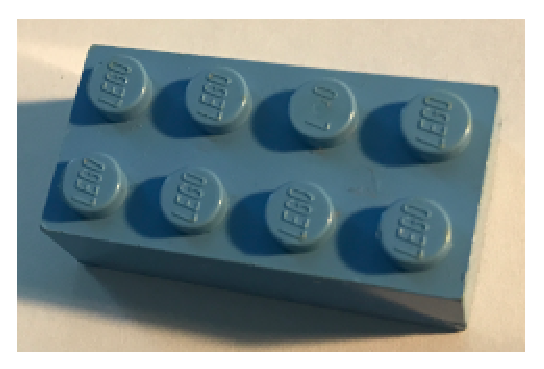
\includegraphics[width=3.5cm]{lego_4_2}
      \end{minipage}
      \partie[]
         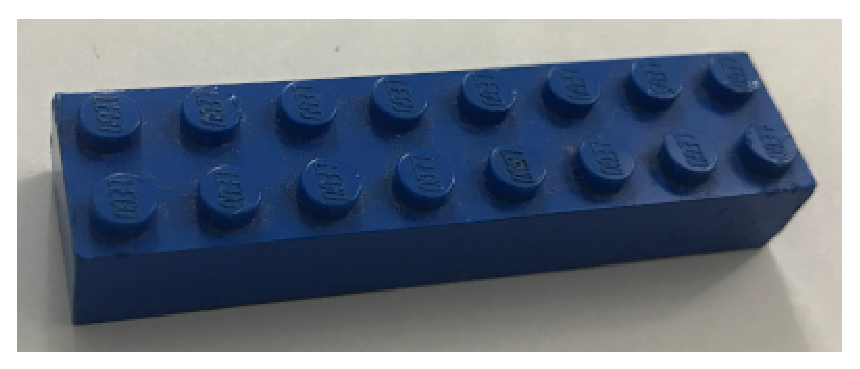
\includegraphics[height=2cm]{lego_8_2}
         \hspace{2.6cm}
         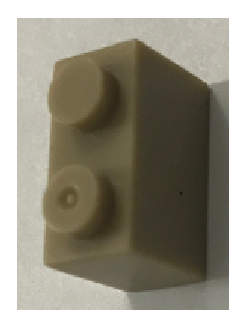
\includegraphics[height=2cm]{lego_2_1}
         \hspace{4.8cm}
         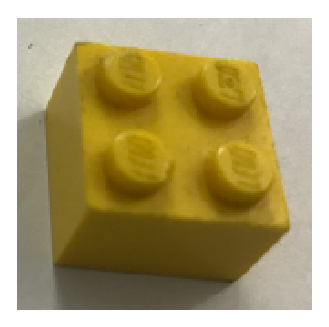
\includegraphics[height=2cm]{lego_2_2} \\ [2.5mm]
         \pf \hfill \pf \hfill \pf \\ [2.5mm]
         \pf \hfill \pf \hfill \pf \smallskip

      \partie[]
         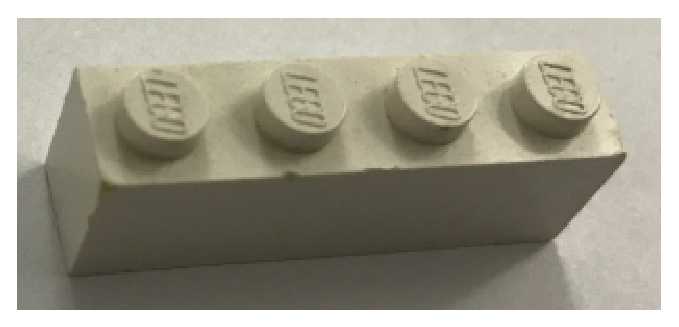
\includegraphics[height=2cm]{lego_4_1}
         \hspace{1.3cm}
         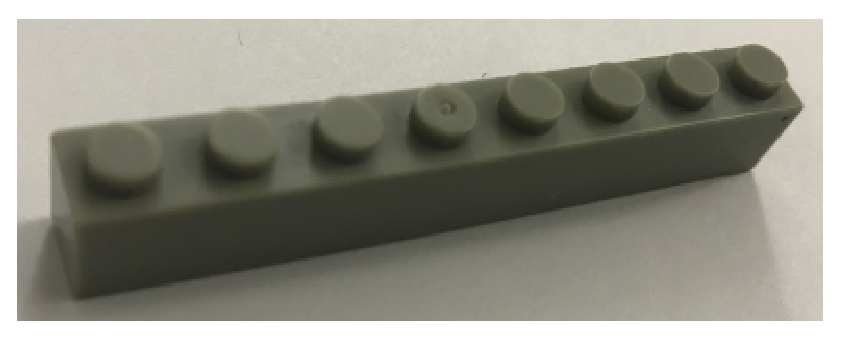
\includegraphics[height=2cm]{lego_8_1}
         \hspace{2.7cm}
         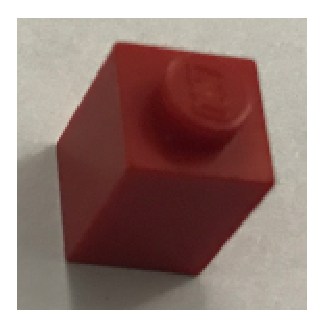
\includegraphics[height=2cm]{lego_1_1} \\ [2.5mm]
         \pf \hfill \pf \hfill \pf \\ [2.5mm]
         \pf \hfill \pf \hfill \pf \smallskip
         
      \partie[]
         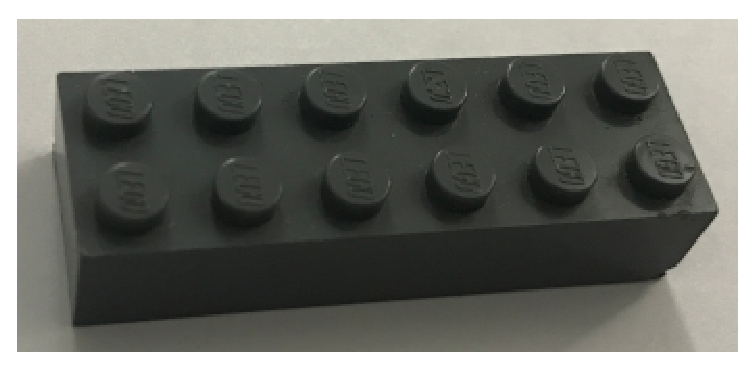
\includegraphics[height=2cm]{lego_6_2}
         \hspace{2.8cm}
         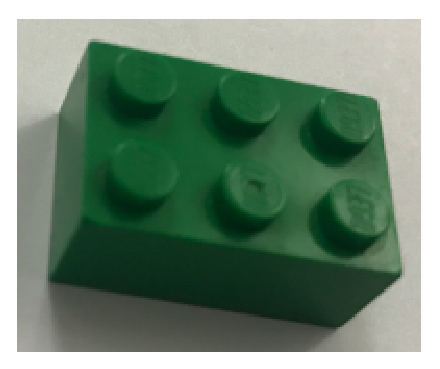
\includegraphics[height=2cm]{lego_3_2}
         \hspace{2.5cm}
         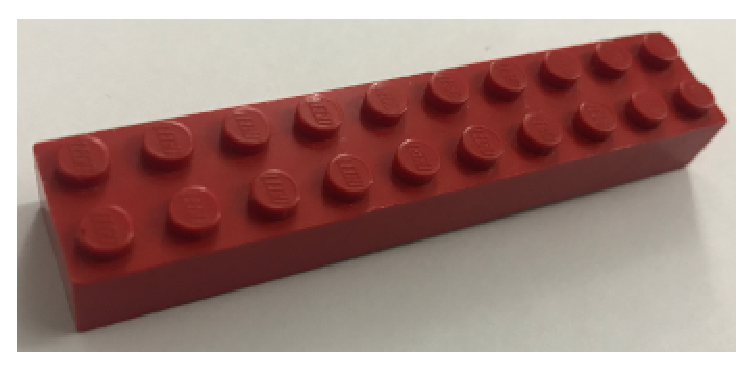
\includegraphics[height=2cm]{lego_10_2} \\ [2.5mm]
         \pf \hfill \pf \hfill \pf \\ [2.5mm]
         \pf \hfill \pf \hfill \pf \smallskip
      
      \partie[]
         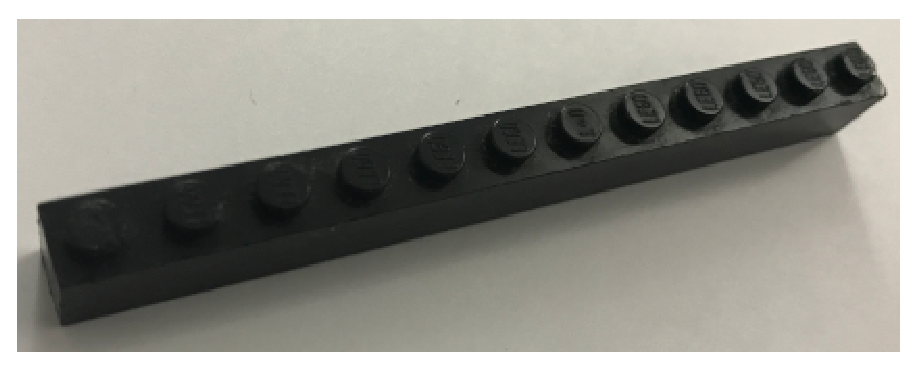
\includegraphics[height=2cm]{lego_12_1}
         \hspace{0.5cm}
         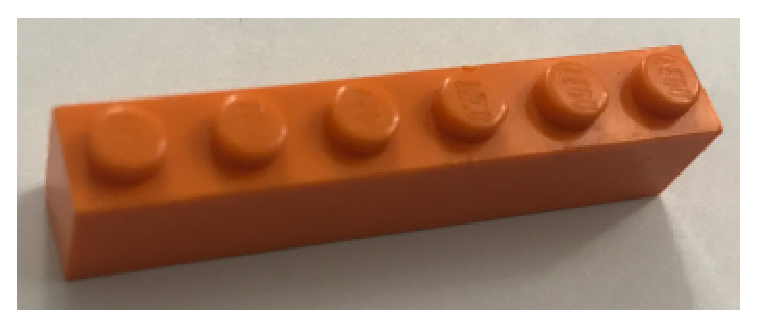
\includegraphics[height=2cm]{lego_6_1}
         \hspace{2cm}
         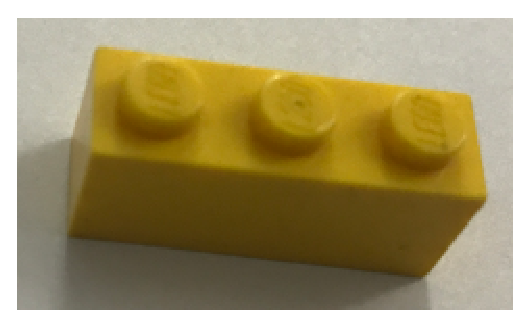
\includegraphics[height=2cm]{lego_3_1} \\ [2.5mm]
         \pf \hfill \pf \hfill \pf \\ [2.5mm]
         \pf \hfill \pf \hfill \pf \medskip
   \end{QCM}
\end{activite}
   

%%%%%%%%%%%%%%%%%%%%%%%%%%%%%%%%%%%%
%%%%%%%%%%%%%%%%%%%%%%%%%%%%%%%%%%%%
\cours 

%%%%%%%%%%%%%%%%%%%%%%%%%%
\section{Différentes manière de penser les fractions}

\begin{definition}
   Une \textbf{fraction} indique quelle partie d'un tout on doit prendre, elle peut représenter un {\bf partage}, une {\bf proportion}.
\end{definition}

\bigskip

On partage une pizza en quatre parts égales.

\begin{center}
   {\small
   \begin{tabular}{C{3}C{3}C{3.5}C{4}}
      \begin{pspicture}(-1,-1.1)(1,1.1)
         \rput(0,0){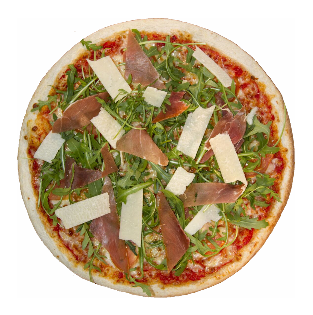
\includegraphics[width=2cm]{pizza}}
         \pscircle(0,0){1}
         \psset{linecolor=white,fillstyle=solid,fillcolor=white}
         \pswedge(0,0){0.98}{90}{0}
         \psset{linecolor=black}
         \psline(-1,0)(1,0)
         \psline(0,-1)(0,1)  
      \end{pspicture}
      &
      \begin{pspicture}(-1,-1.1)(1,1.1)
         \rput(0,0){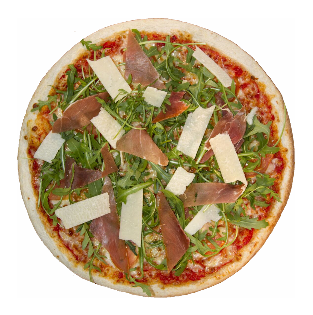
\includegraphics[width=2cm]{pizza}}
         \pscircle(0,0){1}
        \psset{linecolor=white,fillstyle=solid,fillcolor=white}
         \pswedge(0,0){0.98}{180}{0}
         \psline[linewidth=0.7mm](0,0)(0,1) 
         \psset{linecolor=black}
         \psline(-1,0)(1,0)
         \psline(0,-1)(0,0)  
      \end{pspicture}
      &
      \begin{pspicture}(-1,-1.1)(1,1.1)
         \rput(0,0){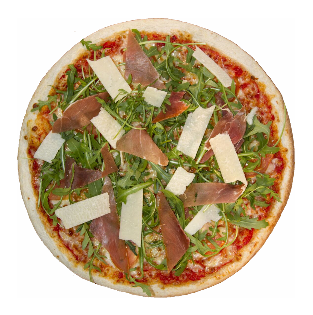
\includegraphics[width=2cm]{pizza}}
         \pscircle(0,0){1}
         \psset{linecolor=white,fillstyle=solid,fillcolor=white}
         \pswedge(0,0){0.98}{-90}{0}
         \psline[linewidth=0.7mm](-1,0)(1,0)
         \psline[linewidth=0.7mm](0,0)(0,1)
      \end{pspicture}
      &
      \begin{pspicture}(-1,-1.1)(1,1.1)
         \rput(0,0){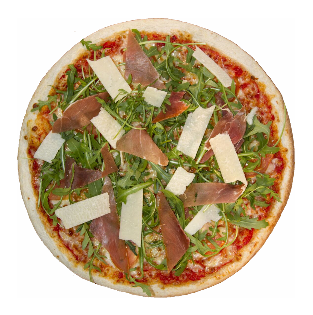
\includegraphics[width=2cm]{pizza}}
        \pscircle(0,0){1}
         \psset{linewidth=0.7mm,linecolor=white}
         \psline(-1,0)(1,0)
         \psline(0,-1)(0,1) 
      \end{pspicture} \\
      {\bf une} part & \textbf{deux} parts & \textbf{trois} parts & \textbf{quatre} parts \\   
      un {\bf quart} de pizza & deux {\bf quarts} de pizza & trois {\bf quarts} de pizza & quatre {\bf quarts} de pizza \\ [2mm]
      $\dfrac14$ & $\dfrac24 =\dfrac14+\dfrac14 =2\times\dfrac14$ & $\dfrac34 =\dfrac14+\dfrac14+\dfrac14 =3\times\dfrac14$ & $\dfrac44 =\dfrac14+\dfrac14+\dfrac14+\dfrac14 =4\times\dfrac14$ \\ 
   \end{tabular}}
\end{center}

\smallskip

\begin{minipage}{10cm}
   Et si on mangeait plus d'une pizza ? \\
   Dans ce cas, on obtient une fraction supérieure à 1. \\
   On a pris {\bf sept} parts de pizza, soit $\dfrac74$ de pizza. \\
   On peut aussi dire {\bf une} pizza et {\bf trois} quarts de pizza, soit $1+\dfrac34$.
\end{minipage}
\qquad
\begin{minipage}{6cm}
   \begin{pspicture}(-1,-1.2)(1,1.2)
      \rput(0,0){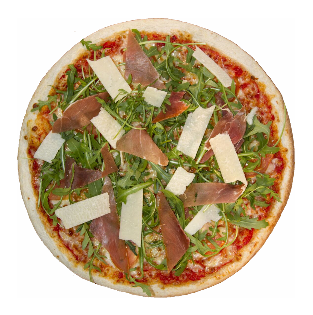
\includegraphics[width=2cm]{pizza}}
      \pscircle(0,0){1}
      \psset{linewidth=0.7mm,linecolor=white}
      \psline(-1,0)(1,0)
      \psline(0,-1)(0,1) 
   \end{pspicture}
   \qquad 
   \begin{pspicture}(-1,-1.2)(1,1.2)
      \rput(0,0){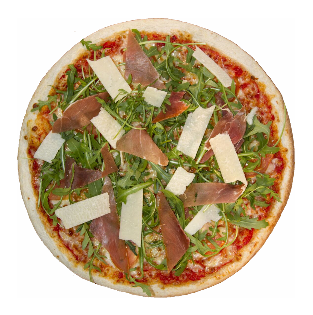
\includegraphics[width=2cm]{pizza}}
      \pscircle(0,0){1}
      \psset{linecolor=white,fillstyle=solid,fillcolor=white}
      \pswedge(0,0){0.98}{-90}{0}
      \psline[linewidth=0.7mm](-1,0)(1,0)
      \psline[linewidth=0.7mm](0,0)(0,1)
   \end{pspicture}
\end{minipage}


\begin{definition}
   Soit $a$ et $b$ deux nombres ($b\neq0$). Le {\bf quotient} $\dfrac{a}{b}$ est le nombre qui, multiplié par $b$, donne $a$. \\
   Ce quotient écrit sous forme d'une fraction est le résultat d'une division : $\dfrac{a}{b} =a\div b$.
\end{definition}

\begin{exemple}
   La fraction $\dfrac73$ peut être interprétée comme :
   \correction
   \ \\ [-10mm]
   \begin{itemize}
      \item $7\div3$, dont une valeur approchée est 2,33 ;
      \item sept tiers ;
      \item le nombre qui, multiplié par $3$, donne $7$.
   \end{itemize}
\end{exemple}

\begin{remarque} 
   quand on partage une quantité en 
   \begin{itemize}
      \item  \textbf{deux} parts égales, on obtient des \textbf{demis}, le \textbf{double} d'un demi fait un.
      \item \textbf{trois} parts égales, on obtient des \textbf{tiers}, le \textbf{triple} d'un tiers fait un.
      \item \textbf{quatre} parts égales, on obtient des \textbf{quarts}, le \textbf{quadruple} d'un quart fait un.
   \end{itemize}
\end{remarque}


%%%%%%%%%%%%%%%%%%%%%%%%%%%%%%%%
\section{Repérage sur une demi-droite graduée}

Comme tous les autres nombres, on peut placer les fractions sur une droite graduée.

\begin{exemple*1}
   Si on partage l'unité d'une droite graduée en quatre, on peut placer des \og quarts \fg.
   \begin{center}
   \begin{pspicture}(0,0.2)(13,0.7)
      \psaxes[dx=1,yAxis=false,labels=none]{->}(0,0)(13,0)
      \rput(0,-0.3){0}
      \rput(4,-0.3){1}
      \rput(8,-0.3){2}
      \rput(12,-0.3){3}
      \uput[u](0,.1){$\frac04$}
      \uput[u](1,.1){$\frac14$}
      \uput[u](2,.1){$\frac24$}
      \uput[u](3,.1){$\frac34$}
      \uput[u](4,.1){$\frac44$}
      \uput[u](5,.1){$\frac54$}
      \uput[u](6,.1){$\frac64$}
      \uput[u](7,.1){$\frac74$}
      \uput[u](8,.1){$\frac84$}
      \uput[u](9,.1){$\frac94$}
      \uput[u](10,.1){$\frac{10}{4}$}
      \uput[u](11,.1){$\frac{11}{4}$}
      \uput[u](12,.1){$\frac{12}{4}$}
   \end{pspicture}
   \end{center}
\end{exemple*1}


%%%%%%%%%%%%%%%%%%%%%%%%%%%%%%%%%%%%%%%%%%
\exercicesbase

\begin{colonne*exercice}

\serie{Fractions}

\begin{exercice} %1
   Ecrire la fraction qui représente la partie colorée de chaque figure ci-dessous :
   \begin{center}
      \psset{unit=0.65}
      \begin{pspicture}(-1,-1.5)(2,1)
         \psframe[fillstyle=solid,fillcolor=A2](0,0)(-1,-1)
         \psframe(-1,-1)(1,1)
         \psline(-1,0)(1,0)
         \psline(0,-1)(0,1)
         \rput(-1.4,0){$a$}
      \end{pspicture}
      \begin{pspicture}(-1,-1.5)(2,1)
         \pspolygon[fillstyle=solid,fillcolor=A2](0,0)(0,-1)(1,-1)(1,1)(1,1)(-1,1)(-1,0)
         \psframe(-1,-1)(1,1)
         \psline(-1,0)(1,0)
         \psline(0,-1)(0,1)
         \rput(-1.4,0){$b$}
      \end{pspicture}
      \begin{pspicture}(-1,-1.5)(2,1)
         \psframe[fillstyle=solid,fillcolor=A2](-1,-1)(1,0)
         \psframe(-1,-1)(1,1)
         \psline(-1,0)(1,0)
         \psline(0,-1)(0,1)
         \rput(-1.4,0){$c$}
      \end{pspicture}
      \begin{pspicture}(-1,-1.5)(1,1)
         \psframe[fillstyle=solid,fillcolor=A2](-1,-1)(1,1)
         \psline(-1,0)(1,0)
         \psline(0,-1)(0,1)
         \rput(-1.4,0){$d$}
      \end{pspicture}
      
      \begin{pspicture}(-1,-1.5)(2,1)
         \pswedge[fillstyle=solid,fillcolor=B2](0,0){1}{30}{-30}
         \pscircle(0,0){1}
         \multido{\n=0+30}{12}{\psline(0,0)(1;\n)}
         \rput(-1.4,0){$e$}
      \end{pspicture}
      \begin{pspicture}(-1,-1.5)(2,1)
         \pswedge[fillstyle=solid,fillcolor=B2](0,0){1}{90}{180}
         \pscircle(0,0){1}
         \multido{\n=0+30}{12}{\psline(0,0)(1;\n)}
         \rput(-1.4,0){$f$}
      \end{pspicture}
      \begin{pspicture}(-1,-1.5)(2,1)
         \pswedge[fillstyle=solid,fillcolor=B2](0,0){1}{-120}{-60}
         \pscircle(0,0){1}
         \multido{\n=0+30}{12}{\psline(0,0)(1;\n)}
         \rput(-1.4,0){$g$}
      \end{pspicture}
      \begin{pspicture}(-1,-1.5)(1,1)
         \pswedge[fillstyle=solid,fillcolor=B2](0,0){1}{60}{-120}
         \pscircle(0,0){1}
         \multido{\n=0+30}{12}{\psline(0,0)(1;\n)}
         \rput(-1.4,0){$h$}
      \end{pspicture}
      
      \begin{pspicture}(-1,-1.2)(2,1.3)
         \pspolygon[fillstyle=solid,fillcolor=H1](1.2;210)(0,-0.6)(1.2;90)
         \pspolygon(1.2;-30)(1.2;90)(1.2;210)
         \psline(0.6;150)(1.2;-30)
         \psline(0.6;30)(1.2;210)
         \psline(0,-0.6)(0,1.2)
         \rput(-1.4,0.25){$i$}
      \end{pspicture}
      \begin{pspicture}(-1,-1.2)(2,1.3)
         \pspolygon[fillstyle=solid,fillcolor=H1](0,0)(1.2;-30)(0,-0.6)
         \pspolygon[fillstyle=solid,fillcolor=H1](0,0)(1.2;210)(0.6;150)
         \pspolygon[fillstyle=solid,fillcolor=H1](0,0)(1.2;90)(0.6;30)
         \pspolygon(1.2;-30)(1.2;90)(1.2;210)
         \psline(0.6;150)(1.2;-30)
         \psline(0.6;30)(1.2;210)
         \psline(0,-0.6)(0,1.2)
         \rput(-1.4,0.25){$j$}
      \end{pspicture}
      \begin{pspicture}(-1,-1.2)(2,1.3)
         \pspolygon[fillstyle=solid,fillcolor=H1](0,0)(0.6;30)(1.2;90)(0.6;150)
         \pspolygon(1.2;-30)(1.2;90)(1.2;210)
         \psline(0.6;150)(1.2;-30)
         \psline(0.6;30)(1.2;210)
         \psline(0,-0.6)(0,1.2)
         \rput(-1.4,0.25){$k$}
      \end{pspicture}
      \begin{pspicture}(-1,-1.2)(1,1.3)
         \pspolygon[fillstyle=solid,fillcolor=H1](0,0)(0.6;30)(1.2;90)(1.2;210)(1.2;-30)
         \pspolygon(1.2;-30)(1.2;90)(1.2;210)
         \psline(0.6;150)(1.2;-30)
         \psline(0.6;30)(1.2;210)
         \psline(0,-0.6)(0,1.2)
         \rput(-1.4,0.25){$l$}
      \end{pspicture}
      
      \begin{pspicture}(-1,-1.5)(2,1)
         \psgrid[subgriddiv=2,subgridcolor=black,subgridwidth=0.8pt,gridlabels=0](-1,-1)(1,1)
         \psframe[fillstyle=solid,fillcolor=J1](-1,0)(0,1)
         \rput(-1.4,0){$m$}
      \end{pspicture}
      \begin{pspicture}(-1,-1.5)(2,1)
         \psgrid[subgriddiv=2,subgridcolor=black,subgridwidth=0.8pt,gridlabels=0](-1,-1)(1,1)
         \psframe[fillstyle=solid,fillcolor=J1](-1,0)(0,1)
         \psframe[fillstyle=solid,fillcolor=J1](0,0.5)(0.5,0)
         \psframe[fillstyle=solid,fillcolor=J1](-1,-0.5)(-0.5,0)
         \rput(-1.4,0){$n$}
      \end{pspicture}
      \begin{pspicture}(-1,-1.5)(2,1)
         \psgrid[subgriddiv=2,subgridcolor=black,subgridwidth=0.8pt,gridlabels=0](-1,-1)(1,1)
         \psframe[fillstyle=solid,fillcolor=J1](-1,-1)(1,0)
         \psframe[fillstyle=solid,fillcolor=J1](-1,0)(0,1)
         \psframe[fillstyle=solid,fillcolor=J1](0,0)(0.5,0.5)
         \rput(-1.4,0){$p$}
      \end{pspicture}
      \begin{pspicture}(-1,-1.5)(1,1)
         \psgrid[subgriddiv=2,subgridcolor=black,subgridwidth=0.8pt,gridlabels=0](-1,-1)(1,1)
         \psframe[fillstyle=solid,fillcolor=J1](-1,-1)(0.5,0)
         \psframe[fillstyle=solid,fillcolor=J1](-1,0)(-0.5,1)
         \psframe[fillstyle=solid,fillcolor=J1](0.5,-0.5)(1,0)
         \rput(-1.4,0){$q$}
      \end{pspicture}
      
   \end{center}
\end{exercice}
   
\begin{exercice} %2
   Dans chaque figure ci-dessous, colorier selon la fraction donnée.
   \begin{center}
   \small
      \psset{unit=0.9}
      \begin{pspicture}(-1,-1.3)(1.7,1)
         \psframe(-1,-1)(1,1)
         \rput(1.25,0){$\dfrac13$}
      \end{pspicture}
      \begin{pspicture}(-1,-1.3)(1.7,1)
         \psframe(-1,-1)(1,1)
         \rput(1.25,0){$\dfrac34$}
      \end{pspicture}
      \begin{pspicture}(-1,-1.3)(1.5,1)
         \psframe(-1,-1)(1,1)
         \rput(1.25,0){$\dfrac58$}
      \end{pspicture}
      
      \begin{pspicture}(-1,-1.3)(1.7,1)
         \pscircle(0,0){1}
         \rput(1.25,0){$\dfrac13$}
      \end{pspicture}
      \begin{pspicture}(-1,-1.3)(1.7,1)
         \pscircle(0,0){1}
         \rput(1.25,0){$\dfrac34$}
      \end{pspicture}
      \begin{pspicture}(-1,-1.3)(1.5,1)
         \pscircle(0,0){1}
         \rput(1.25,0){$\dfrac58$}
      \end{pspicture}
      
      \begin{pspicture}(-1,-1.3)(1.7,1)
         \pspolygon(1;30)(1;90)(1;150)(1;210)(1;270)(1;330)
         \rput(1.25,0){$\dfrac13$}
      \end{pspicture}
      \begin{pspicture}(-1,-1.3)(1.7,1)
         \pspolygon(1;30)(1;90)(1;150)(1;210)(1;270)(1;330)
         \rput(1.25,0){$\dfrac34$}
      \end{pspicture}
      \begin{pspicture}(-1,-1.3)(1.5,1)
         \pspolygon(1;30)(1;90)(1;150)(1;210)(1;270)(1;330)
         \rput(1.25,0){$\dfrac56$}
      \end{pspicture}

      \begin{pspicture}(-1,-1.3)(1.7,1)
         \pspolygon(-1,-0.33)(-1,0.33)(-0.33,0.33)(-0.33,1)(0.33,1)(0.33,0.33)(1,0.33)(1,-0.33)(0.33,-0.33)(0.33,-1)(-0.33,-1)(-0.33,-0.33)
         \rput(1.25,0){$\dfrac14$}
      \end{pspicture}
      \begin{pspicture}(-1,-1.3)(1.7,1)
         \pspolygon(-1,-0.33)(-1,0.33)(-0.33,0.33)(-0.33,1)(0.33,1)(0.33,0.33)(1,0.33)(1,-0.33)(0.33,-0.33)(0.33,-1)(-0.33,-1)(-0.33,-0.33)
         \rput(1.25,0){$\dfrac38$}
      \end{pspicture}
      \begin{pspicture}(-1,-1.3)(1.5,1)
         \pspolygon(-1,-0.33)(-1,0.33)(-0.33,0.33)(-0.33,1)(0.33,1)(0.33,0.33)(1,0.33)(1,-0.33)(0.33,-0.33)(0.33,-1)(-0.33,-1)(-0.33,-0.33)
         \rput(1.25,0){$\dfrac25$}
      \end{pspicture}
   \end{center}
\end{exercice}

\begin{exercice} %3
   Écrire chaque désignation sous la forme d'une fraction, d'une somme de fractions et d'un produit comme dans l'exemple : $\dfrac24 =\dfrac14+\dfrac14 =2\times\dfrac14$. \smallskip
   \begin{colenumerate}{2}
      \item trois cinquièmes
      \item quatre tiers
      \item cinq septièmes
      \item six centièmes
   \end{colenumerate}
\end{exercice}

\begin{exercice} %4
   Sur la figure suivante, on a représenté un réseau de droites parallèles et équidistantes ainsi qu'un segment de longueur $u$ à trois reprises. À l'aide du compas, tracer sur le cahier les segments de longueur suivante :
   \smallskip
   \begin{colenumerate}{6}
      \item $\dfrac16u$
      \item $\dfrac15u$
      \item $\dfrac13u$
      \item $\dfrac56u$
      \item $\dfrac23u$
      \item $\dfrac35u$
   \end{colenumerate}
   \medskip
   \psset{xunit=0.7,yunit=0.3}
   \begin{pspicture*}(0,0)(11,8)
      \multido{\n=-3+1,\i=1+1}{14}{\psline[linecolor=gray](\n,0)(\i,8)}
       \psline[linewidth=0.5mm]{|-|}(0.5,3)(5.8,7.6)
      \psline[linewidth=0.5mm]{|-|}(2,2)(8.4,4.8)
      \psline[linewidth=0.5mm]{|-|}(3.5,1)(10.3,2.6)
      \rput(10.6,2.6){$u$}
      \rput(8.7,4.8){$u$}
      \rput(6.2,7.6){$u$}
   \end{pspicture*}
\end{exercice}

\begin{exercice} %5
   Compléter les phrases ci-dessous avec des mots.
   \begin{enumerate}
      \item 6 mois représentent \pf année.
      \item 4 mois représentent \pf année.
      \item 30 minutes représentent \pf heure.
      \item 45 minutes représentent \pf heure.
   \end{enumerate}
\end{exercice}

\medskip

\begin{exercice} %6
   Par quel nombre faut-il :
   \begin{enumerate}
      \item multiplier 5 pour obtenir 3 ?
      \item multiplier 19 pour obtenir 97 ?
      \item multiplier 12 pour obtenir 11 ?
   \end{enumerate}
\end{exercice}

%%%%%%%%%%%%%
\serie{Repérage}

\begin{exercice} %7
   Écrire l'abscisse de chaque point à l'aide d'une ou plusieurs fractions.
   {\small
   \begin{enumerate}
      \item \begin{pspicture}(0,0)(8,0.7)
                  \psset{xunit=5}
                  \psaxes[yAxis=false,subticks=10,subtickwidth=0.7pt]{->}(0,0)(1.5,0)
                  \pstGeonode[PosAngle=90](0.3,0){A}(0.8,0){C}(1.1,0){D}(1.3,0){B}
               \end{pspicture}
      \item \begin{pspicture}(0,0)(8,1.2)
                  \psset{xunit=3}
                  \psaxes[yAxis=false,subticks=5,subtickwidth=0.7pt]{->}(0,0)(2.5,0)
                  \pstGeonode[PosAngle=90](0.2,0){F}(0.6,0){E}(2.2,0){G}(1.8,0){H}
               \end{pspicture}
      \item \begin{pspicture}(0,0)(8,1.2)
                  \psset{xunit=4}
                  \psaxes[yAxis=false,subticks=8,subtickwidth=0.7pt]{->}(0,0)(1.9,0)
                  \pstGeonode[PosAngle=90](0.25,0){J}(1.125,0){K}(1.5,0){L}(0.625,0){M}
               \end{pspicture}
      \item \begin{pspicture}(0,-0.5)(8,1.2)
                  \psset{xunit=3}
                  \psaxes[yAxis=false,subticks=12,subtickwidth=0.7pt]{->}(0,0)(2.5,0)
                  \pstGeonode[PosAngle=90](0.25,0){P}(1.67,0){Q}(1,0){N}(2.08,0){R}
               \end{pspicture}
   \end{enumerate}}
\end{exercice}

\medskip

\begin{exercice} %8
   Placer les points donnés sur chaque demi-droite.
   \smallskip
   {\small
   \begin{enumerate}
      \item $S\left(\dfrac56\right)$ \; ; \; $T\left(\dfrac26\right)$ \; ; \; $U\left(\dfrac96\right)$ \; et \; $V\left(\dfrac66\right)$. \\
        \begin{pspicture}(0,-0.5)(8,0.5)
           \psset{xunit=4}
           \psaxes[yAxis=false,subticks=6,subtickwidth=0.7pt]{->}(0,0)(1.9,0)
        \end{pspicture}
        \item $W\left(\dfrac{7}{15}\right)$ \; ; \; $X\left(\dfrac{17}{15}\right)$ \; ; \; $Y\left(\dfrac{3}{15}\right)$ \; et \; $Z\left(\dfrac{10}{15}\right)$. \\
        \begin{pspicture}(0,-0.5)(8,0.5)
           \psset{xunit=5}
           \psaxes[yAxis=false,subticks=15,subtickwidth=0.7pt]{->}(0,0)(1.4,0)
        \end{pspicture} 
   \end{enumerate}}
\end{exercice}

\end{colonne*exercice}


%%%%%%%%%%%%%%%%%%%%%%%%%%%%%%%
%%%%%%%%%%%%%%%%%%%%%%%%%%%%%%%
\Recreation
   \enigme[L'atelier des potions]
      \partie[présentation du jeu]
         L’atelier des potions est un jeu innovant, basé sur la manipulation, qui permet un enseignement et un apprentissage ludique et concret des fractions. \\  
Il a été conçu de façon collaborative par des chercheurs et des enseignants, dans le but d'être facilement utilisable en classe, en petits groupes ou en classe entière. \\
         \begin{center}
           \includegraphics[width=11cm]{potions}
         \end{center}

      \partie[principes du jeu]
         Les élèves, apprentis sorciers, réalisent des potions en sélectionnant la bonne fraction d’ingrédient parmi ceux à leur disposition. Les cartes, ordonnées suivant un ordre croissant de difficulté, permettent de travailler les notions suivantes :
         \begin{itemize}
            \item représentation de fractions ;
            \item fractions supérieures à 1 ;
            \item équivalence de fraction ;
            \item somme de fractions ;
            \item décomposition de fractions, etc.
         \end{itemize}
         \begin{center}
            \includegraphics[width=4cm]{carte}
         \end{center}

\begin{flushright}
   \href{https://www.atelier-potions.fr}{{\small https://www.atelier-potions.fr}}
\end{flushright}

\themaG
\graphicspath{{../Ch5_Le_cercle/Images/}}

\chapter{Cercles et disques}
\label{C12}


%%%%%%%%%%%%%%%%%%%%%%%%%%%%%%%%%%%%%%%%%%
\begin{prerequis}[Connaissances et compétences abordées]
   \begin{itemize}
      \item Reconnaître, nommer le cercle (comme ensemble des points situés à une distance donnée d’un point donné), le disque.
      \item Vocabulaire associé au cercle et à leurs propriétés : centre, rayon, diamètre, milieu.
   \end{itemize}
\end{prerequis}

\vfill

\begin{debat}[Débat : les crop circle] 
   Un {\bf cercle de culture} (traduction de {\bf crop circle}), ou {\bf agrogramme} ou encore {\bf agroglyphe} est un très grand motif ou un ensemble de motifs géométriques réalisé dans un champ de céréales en couchant les épis au sol, ils sont apparus pour la première fois dans les années 1970. Ces formes impressionnantes sont visibles depuis le ciel. Pendant plusieurs années, on croyait que leur origine était extra-terrestre jusqu'à ce que l'on découvre leur vraie origine\dots{} terrestre.
   \begin{center} 
      \includegraphics[width=5cm]{crop}
   \end{center}
   \bigskip
   \begin{cadre}[B2][F4]
      \begin{center}
         Vidéo : \href{https://www.francetvinfo.fr/replay-jt/france-2/20-heures/video-en-alsace-les-mysterieux-cercles-dans-le-champ-etaient-un-cours-de-maths_3505711.html}{\bf Les mystérieux cercles dans le champ étaient un cours de maths}, {\it franceinfo}, émission {\it L'Oeil du 20 h}.
      \end{center}
   \end{cadre}
\end{debat}

\vfill

\textcolor{PartieGeometrie}{\sffamily\bfseries Cahier de compétences} : chapitre 7, exercices 16 à 21 ; 25.


%%%%%%%%%%%%%%%%%%%%%%%%%%%%%%%%%%%%
%%%%%%%%%%%%%%%%%%%%%%%%%%%%%%%%%%%%
\activites

   \begin{activite}[Tracer des cercles avec GeoGebra]
      {\bf Objectif :} construire un point ; un cercle ; une figure complexe avec un logiciel de géométrie dynamique.
      \begin{QCM}
         Ouvrir Geogebra et choisir l'onglet \textbf{Géométrie}. \\
         \partie[placer un point et le renommer]
            Dans la barre d'outils, sélectionner le menu relatif aux points :
            \begin{pspicture}(-0.5,-0.5)(0.5,0)
               \psframe[framearc=0.2,linecolor=lightgray](-0.5,-0.5)(0.5,0.5)
               \psdot[linecolor=blue,linewidth=0.6mm](-0.15,-0.15)   
               \rput(0.15,0.15){\blue A}
            \end{pspicture} \\
            Choisir l'item \og Point \fg{} puis cliquer sur l'écran, que se passe-t-il ? \\ [1mm]
            \pf \\ [2mm]
            Déplacer le point grâce à l'outil \og Déplacer \fg :
            \begin{pspicture}(-0.5,-0.1)(0.5,.5)
               \psframe[framearc=0.2,linecolor=lightgray](-0.5,-0.5)(0.5,0.5)
               \pspolygon(0.15,-0.35)(0.26,-0.28)(0.01,0.1)(0.2,0.12)(-0.2,0.34)(-0.2,-0.12)(-0.1,0.03)
            \end{pspicture} \\

            Faire un clic droit sur le point et choisir \og Propriétés \fg. Changer le nom du point en O. \\
         
         \partie[tracer un cercle]
            Dans la barre d'outils, sélectionner le menu relatif aux cercles :
            \begin{pspicture}(-0.5,-0.5)(0.5,0)
               \psframe[framearc=0.2,linecolor=lightgray](-0.5,-0.5)(0.5,0.5)
               \psdots[linecolor=blue](0,0)(0.3;60)
               \pscircle(0,0){0.3}       
            \end{pspicture}. Que contient ce menu ? \\ [1mm]
                \pf \\ [2mm]
               \pf \\ [2mm]
            Il existe trois façons de tracer un cercle :
            \begin{center}
               \newcolumntype{M}{>{\itshape\footnotesize}p{5cm}}
               \begin{tabular}{|c|p{6cm}|p{2.5cm}|M|}
                  \hline
                  & Instructions & outil du menu & action \\
                  \hline
                  1 & \multicolumn{3}{l|}{On a le {\bf centre} et un {\bf point} du cercle} \\
                  \hdashline
                  & Placer un point O sur l'écran & Point & placer le point sur l'écran puis changer son nom \\
                  & Placer un point A sur l'écran & Point & placer le point sur l'écran puis changer son nom \\
                  & Tracer le cercle de centre O passant par A & Cercle\newline(centre-point) & sélectionner O, puis A \\
                  & Faire bouger A et O & Déplacer & sélectionner O ou A et les faire bouger \\
                  \hline
                  2 & \multicolumn{3}{l|}{On a le centre et le rayon du cercle} \\
                  \hdashline
                  & Placer un point B sur l'écran & & \\
                  & Tracer le cercle de centre B de rayon \ucm{3} & Cercle\newline(centre-rayon) & sélectionner B, puis entrer la valeur du rayon \\
                  & Faire bouger B & & \\
                  \hline
                  3 & \multicolumn{3}{l|}{On a trois points du cercle} \\
                  \hdashline
                  & Placer trois points C, L et E & Point & \\
                  & Tracer le cercle passant par C, L et E & Cercle (passant\newline par trois points) & sélectionner successivement, C, L et E \\
                  \hline
               \end{tabular}
            \end{center} \medskip
        
         \partie[défi !!!]
            Dessiner un bonhomme de neige : il est tout à fait possible d'explorer les autres menus de GeoGebra et de faire preuve de créativité. Le menu propriétés (clic droit) permet de colorier la figure ou de la remplir de motifs. \medskip
      \end{QCM}
   \end{activite}
   
   
%%%%%%%%%%%%%%%%%%%%%%%%%%%%%%%%%%%%
%%%%%%%%%%%%%%%%%%%%%%%%%%%%%%%%%%%%
\cours 

%%%%%%%%%%%%%%%%%%%%%%%%%%%%%%%%%%%%
\section{Le cercle, le disque}

\begin{definition}
   Le \textbf{cercle} de centre O de rayon $r$ est l'ensemble des points situés à une distance $r$ du point O. \\ 
   Le \textbf{disque} est l'intérieur du cercle.
\end{definition}

{\psset{unit=0.6}
\begin{pspicture}(-5,0.1)(10,4.9)
   \psdots(2,2)
   \rput(2,1.6){$O$}
   \psarc(2,2){2}{70}{-45}
   \psarc[linestyle=dashed](2,2){2}{-45}{70}
   \psline[linecolor=B1,arrowsize=0.25]{<->}(0,2)(2,2)
   \rput(1,2.3){\textcolor{B1}{$r$}}
   \rput(10,2){\begin{minipage}{3.2cm} Un cercle se dessine en général à l'aide d'un compas. \end{minipage}}
\end{pspicture}}

\begin{definition}
   \begin{itemize}
      \item Un {\bf rayon} d'un cercle est un segment d'extrémité le centre du cercle et un point du cercle, c'est aussi la longueur de ce segment.
      \item Une \textbf{corde} est un segment reliant deux points du cercle.
      \item Lorsqu'une corde passe par le centre du cercle, on l'appelle un \textbf{diamètre} du cercle.
      \item Une partie du cercle comprise entre deux points est appelée \textbf{arc} de cercle.
   \end{itemize}
\end{definition}

\begin{minipage}{9cm}
   \psset{unit=0.9}
   \begin{pspicture}(-3.5,0.2)(4,4.4)
      \psdots(2,2)
      \psarc[linecolor=A1](2,2){2}{180}{240}
      \psarc(2,2){2}{240}{180}
      \rput(2,1.6){$O$}
      \rput(0.4,3.7){$\mathcal{C}$}
      \psline[linecolor=B1](0,2)(2,2)
      \psdots(0,2)
      \rput(-0.3,2){$A$}
      \psdots(3,3.7)
      \rput(3.2,4){$B$}
      \psdots(1,0.3)
      \rput(0.8,-0.2){$C$}
      \psline[linecolor=D1](1,0.3)(3,3.7)
      \psline[linecolor=J1](0,2)(3,3.7)
      \psdots[dotstyle=+](1,2)(2.5,2.85)(1.52,1.2)
   \end{pspicture}
\end{minipage}
\begin{minipage}{7cm}
   \textcolor{B1}{$[OA]$ est un rayon du cercle $\mathcal{C}$.} \\
   \textcolor{D1}{$[BC]$ est un diamètre du cercle $\mathcal{C}$.} \\
   \textcolor{A1}{$\wideparen{AC}$ est un arc du cercle $\mathcal{C}$.} \\
   \textcolor{J1}{$[AB]$ est une corde du cercle $\mathcal{C}$.} \\[3mm]
   On a $OA = OB = OC$ et $BC =2\,OC$ \\
   $O$ est le milieu du segment $[BC]$
\end{minipage}


%%%%%%%%%%%%%%%%%%%%%%%%
\section{Rédiger un programme de construction}

Rédiger un programme de construction signifie écrire des instructions permettant de construire une figure.

\begin{exemple}
   Écrire un programme de construction permettant d'obtenir la figure ci-dessous puis la construire. \\   
   \small\psset{unit=0.5}
   \begin{pspicture}(0,-4)(12,4.5)
      \pscircle(2,0){2}
      \psarc(4,0){4}{0}{180}
      \psarc(8,0){4}{180}{0}
      \pscircle(10,0){2}
      \psdots(0,0)(4,0)(8,0)(12,0)
      \rput(0.4,-0.4){$A$}
      \rput(4.4,-0.43){$B$}
      \rput(8.4,-0.4){$C$}
      \rput(12.4,-0.4){$D$}
      \psline(0,0)(12,0)
      \rput(2,0.7){5 cm}
      \rput(2,0){/\!\!/}
      \rput(6,0){/\!\!/}
      \rput(10,0){/\!\!/}
   \end{pspicture}
   \correction
      - Tracer le segment $[AD]$ de longueur $AD =15$ cm. \\
      - Placer les points $B$ et $C$ sur ce segment tels que $AB =5$ cm et $AC =10$ cm. \\
      - Tracer le cercle de diamètre $[AB]$. \\ 
      - Tracer le demi-cercle de diamètre $[AC]$ situé au-dessus du segment $[AD]$. \\      
      - Tracer le demi-cercle de diamètre $[BD]$ situé en-dessous du segment $[AD]$. \\
      - Tracer le cercle de diamètre $[CD]$. \\ [2mm]
      {\it Attention : un programme de construction n'est pas unique et il ne mentionne pas les instruments à utiliser.}
\end{exemple}

   
%%%%%%%%%%%%%%%%%%%%%%%%%%%%%%%%%
%%%%%%%%%%%%%%%%%%%%%%%%%%%%%%%%%
\exercicesbase

\begin{colonne*exercice}

%%%%%
\serie{Vocabulaire du cercle}

\begin{exercice}
   Compléter les phrases suivantes en utilisant les mots : cercle - corde - rayon - centre - diamètre - milieu.
   \begin{itemize}
      \item Le \pfb ($\mathcal{C}_1$) de \pfb $E$ \\
         passe par les points $A, B, C, D$ et $F$.
      \item Le segment $[EF]$ est un \pf de ce cercle.
      \item Le segment $[AC]$ est une \pf de ce cercle.
      \item $E$ est le \pfb du \pfb $[AD]$.
   \end{itemize}
   \begin{center}
   \psset{unit=0.75}
   \begin{pspicture}(-2,-2.3)(2,2.5)
      \pstGeonode[PointSymbol=none,PosAngle={-135,80,140,220,-60,-40}]{E}(2;80){B}(2;140){A}(2;220){C}(2;-60){F}(2;-40){D}
      \pstCircleOA{E}{A}
      \pstSegmentMark{E}{A}
      \pstSegmentMark{E}{B}
      \pstSegmentMark{E}{D}
      \pstSegmentMark{E}{F}
      \pstLineAB{B}{C}
      \pstLineAB{A}{C}
      \rput(2.5;40){($\mathcal{C}_1$)}
   \end{pspicture}
   \end{center}
\end{exercice}

\begin{exercice}
   Compléter les phrases ci-dessous en utilisant la règle graduée ou le compas.
   \begin{itemize}
      \item Le cercle ($\mathcal{C}_1$) de centre J passant par G passe également par les points \pf et  \pf \\ [-5mm]
      \item Le cercle ($\mathcal{C}_2$) de centre P et de rayon PH passe par les points  \pf,  \pf et  \pf
      \item Les points  \pf,  \pf et  \pf sont sur \\
         le cercle ($\mathcal{C}_3$) de centre F et de rayon EF.
      \item Les points A, F et I sont sur le même cercle ($\mathcal{C}_4$) de centre  \pf
      \item Le point situé à l'intersection des cercles ($\mathcal{C}_2$) et ($\mathcal{C}_4$) est le point  \pf
   \end{itemize}
   \begin{center}
      \includegraphics[width=8cm]{points}
   \end{center}
\end{exercice}

%%%%%
\serie{Programmes de construction}

\begin{exercice}
   Construire les figures suivantes :
   \begin{enumerate}
      \item
      \begin{itemize}
         \item Tracer un cercle ($\mathcal{C}$) de centre O et de rayon 4 cm puis un cercle de rayon 4 cm et passant par O.
         \item Où se trouve le centre du deuxième cercle ?
      \end{itemize}
      \item
      \begin{itemize}
         \item Tracer un segment [AB] de longueur 5 cm.
         \item Tracer le cercle ($\mathcal{C}$) de diamètre [AB].
         \item Quel est le rayon du cercle ($\mathcal{C}$) ?
      \end{itemize}
   \end{enumerate}
\end{exercice}

\begin{exercice}
   {\small Construire un carré} ABCD de côté 8 cm de centre O.
   \begin{itemize}
      \item Placer les points I, J, K et L milieux respectifs de [AB], [BC], [CD] et [DA].
      \item Sur ce carré, tracer chacun des cercles suivants :
      \begin{itemize}
         \item[-] ($\mathcal{C}_1$) de centre O passant par A.
         \item[-] ($\mathcal{C}_2$) de centre O et de rayon 2,5 cm.
         \item[-] ($\mathcal{C}_3$) dont [OD] est un diamètre.
      \end{itemize}
   \end{itemize}
\end{exercice}

\begin{exercice}
   Écrire un programme de construction pour chaque figure puis la construire. \\
   \psset{unit=0.6}
   \small
   \begin{pspicture}(-4,-2)(3,2.3)
      \pscircle(0,0){2}
      \psline{|-}(0,0)(2;45)
      \rput{45}(1,0.3){3,5 cm}
      \rput(-0.3,-0.3){P}
   \end{pspicture}
   \begin{pspicture}(-3,-2)(3,2.3)
      \pscircle(0,0){2}
      \psline{-}(2;180)(2;0)
      \psline[linecolor=gray]{<->}(2;175)(2;5)
      \rput(0,0.6){6,8 cm}
      \rput(0,-0.5){M}
      \rput(0,0){$\times$}
   \end{pspicture}
\end{exercice}

\begin{exercice}
   Écrire un texte pour décrire les différentes étapes de cette construction. \\
   \psset{unit=0.5}
   \footnotesize
   \begin{pspicture}(-3,-2.3)(3,2.3)
      \pscircle(0,0){2}
      \psline{-}(2;180)(2;0)
      \psline{<->}(2;175)(2;5)
      \rput(0,0.6){16 cm}
      \rput(0,-0.5){C}
      \rput(-2.5,0){A}
      \rput(2.5,0){B}
      \rput(0,0){$\times$}
      \rput(0,-2.7){étape 1}
   \end{pspicture}
   \begin{pspicture}(-3,-2.3)(3,2.3)
      \pscircle(0,0){2}
      \psline{-}(2;180)(2;0)
      \rput(-0.2,-0.5){C}
      \rput(1,-0.5){D}
      \rput(-2.5,0){A}
      \rput(2.5,0){B}
      \rput(0,0){$\times$}
      \rput(1,0){$\times$}
      \pscircle(1,0){1}
      \rput(0,-2.7){étape 2}
   \end{pspicture}
   \begin{pspicture}(-3,-2.3)(3,2.3)
      \pscircle(0,0){2}
      \psline{-}(2;180)(2;0)
      \rput(-0.2,-0.5){C}
      \rput(0.9,-0.5){D}
      \rput(-2.5,0){A}
      \rput(2.5,0){B}
      \rput(0,0){$\times$}
      \rput(1,0){$\times$}
      \pscircle(1,0){1}
      \pscircle(1.5,0){0.5}
      \rput(0,-2.7){étape 3}
   \end{pspicture}
\end{exercice}

%%%%%
\serie{Reproduire des figures}

\begin{exercice}
   Reproduire chaque figure sur le cahier. \\
   \psset{unit=0.25}
   \begin{pspicture}(-2,0)(14,16.5)
      \psgrid[griddots=20, subgriddiv=0, gridlabels=0,gridcolor=gray](-2,0)(14,16)
      \psarc(7,1){1}{180}{0}
      \psline(6,1)(6,8)
      \psline(0,10)(6,16)(12,10)
      \psline(4,10)(6,16)(8,10)
      \psarc(2,10){2}{180}{0}
      \psarc(6,10){2}{180}{0}
      \psarc(10,10){2}{180}{0}
   \end{pspicture}
   \begin{pspicture}(0,0)(16,16.5)
      \psgrid[griddots=20, subgriddiv=0, gridlabels=0,gridcolor=gray](0,0)(16,16)
      \psarc(3,3){2}{90}{0}
      \psarc(8,3){3}{0}{180}
      \psarc(13,3){2}{180}{90}
      \psarc(13,8){3}{90}{270}
      \psarc(13,13){2}{-90}{180}
      \psarc(8,13){3}{180}{0}
      \psarc(3,13){2}{0}{270}
      \psarc(3,8){3}{-90}{90}
   \end{pspicture}
\end{exercice}

\end{colonne*exercice}


%%%%%%%%%%%%%%%%%%%%%%%%%%%%%%%%%%%%
\Recreation

   \enigme[Rosaces]
      Dessiner une rosace (sur une feuille unie) puis la colorier et la découper. Elle peut par exemple ressembler à l'une des trois rosaces ci-dessous mais il est aussi possible de faire travailler son imagination !
   \begin{center}
      \begin{pspicture}(-4,-5)(4,5.5)
         \pscircle(0,0){4}
         \multido{\n=0+30,\i=120+30,\r=240+30}{12}{\psarc(4;\n){4}{\i}{\r}}
      \end{pspicture}
      \qquad
      \begin{pspicture}(-4,-5)(4,6)
         \multido{\n=0+30}{12}{\pscircle(2;\n){2}}
      \end{pspicture}
      \begin{pspicture}(-4,-4)(4,4)
         \pscircle(0,0){4}
         \pscircle(0,0){2}
         \pscircle(0,0){3.5}
         \multido{\n=0+60}{6}{\pscircle(2;\n){2}}
      \end{pspicture}
   \end{center}







\themaM
\graphicspath{{../Ch22_Les_angles/Images/}}

\chapter{Angles et degrés}
\label{C13}


%%%%%%%%%%%%%%%%%%%%%%%%%%%%%%%%%%%%%%%%%
%%%%%%%%%%%%%%%%%%%%%%%%%%%%%%%%%%%%%%%%%
\begin{prerequis}[Connaissances et compétences associées]
   \begin{itemize}
      \item Identifier des angles dans une figure géométrique.
      \item Comparer des angles, en ayant ou non recours à leur mesure (par superposition, avec un calque).
      \item Reproduire un angle donné en utilisant un gabarit.
      \item Estimer qu’un angle est droit, aigu ou obtus.
      \item Utiliser l’équerre pour vérifier qu’un angle est droit, aigu ou obtus, ou pour construire un angle droit.
   \end{itemize}
\end{prerequis}

\vfill

\begin{debat}[Débat : angles et perspective]
   La {\bf perspective} est un ensemble de techniques destinées à représenter un objet ou une image en trois dimensions sur une surface plane. Il existe plusieurs sortes de perspectives, comme par exemple la perpective cavalière, la perspective isométrique, la perpective à point de fuite\dots{} Selon la perspective utilisée, on utilise des directions suivant des angles différents.
   \begin{center}
      \begin{pspicture}(0,-1)(4,3.5)
         \psframe(0,0)(1.5,1.5)
         \psline(0,1.5)(0.8,2.3)(2.3,2.3)(2.3,0.8)(1.5,0)
         \psline(1.5,1.5)(2.3,2.3)
         \psset{linestyle=dashed,linecolor=A1}
         \psline(0.8,2.3)(1.6,3.1)
         \psline(2.3,2.3)(3.1,3.1)
         \psline(2.3,0.8)(3.1,1.6)
         \rput(0.75,-0.75){\it cavalière}
      \end{pspicture}
      \begin{pspicture}(-2,-2.5)(2,2)
         \pspolygon(1.3;-30)(1.3;30)(1.3;90)(1.3;150)(1.3;-150)(1.3;-90)
         \psline(1.3;150)(0,0)(1.3;30)
         \psline(0,0)(1.3;-90)
        \psset{linestyle=dashed,linecolor=A1}
         \psline(1.3;150)(2.3;150)
         \psline(1.3;30)(2.3;30)
         \psline(1.3;-90)(2;-90)
         \rput(0,-2.25){\it isométrique}
      \end{pspicture}
      \begin{pspicture}(-1,-1)(3,3.5)
         \psframe(0,0)(1.5,1.5)
         \psline(0,1.5)(0.8,1.9)(1.9,1.9)(1.9,0.8)(1.5,0)
         \psline(1.5,1.5)(1.9,1.9)
         \psdot(3,3)
         \psset{linestyle=dashed,linecolor=A1}
         \psline(0.8,1.9)(3,3)
         \psline(1.9,1.9)(3,3)
         \psline(1.9,0.8)(3,3)
         \rput(0.75,-0.75){\it un point de fuite}
      \end{pspicture}
   \end{center}
   \bigskip
   \begin{cadre}[B2][F4]
      \begin{center}
         Vidéo : \href{https://www.youtube.com/watch?v=zCIxdOCQiZg}{\bf Comment dessiner des illusions d'optique 3D}, chaîne YouTube {\it Simple drawing tutorial}.
      \end{center}
   \end{cadre}
\end{debat}

\vfill

\textcolor{PartieGeometrie}{\sffamily\bfseries Cahier de compétences} : chapitre 8, exercices 1 ; 2 ; 5 ;  6 ; 9.


%%%%%%%%%%%%%%%%%%%%%%%%%%%%%%%%%%%%
%%%%%%%%%%%%%%%%%%%%%%%%%%%%%%%%%%%%
\activites

\begin{activite}[Une nouvelle unité de mesure]
   {\bf Objectif :} comparer des angles sans recours à la mesure ; découvrir le degré ; mesurer un angle donné.
   \begin{QCM}
      \partie[fabrication d'angles]
      {\it Partie à faire en binôme.}
         \begin{enumerate}
            \item 
            \begin{enumerate}
               \item Sur une feuille, construire deux \textbf{carrés} dont les mesures des côtés sont respectivement \ucm{4} et \ucm{7}.
               \item Découper ces carrés puis les plier en deux suivant une \textbf{diagonale} : on obtient pour chaque carré deux triangles identiques à découper.
               \begin{center}
                  {\psset{unit=0.7}
                  \begin{pspicture}(-0.5,-0.3)(4,3)
                     \psframe(0,0)(3,3)
                     \psline[linestyle=dashed](0,0)(3,3)
                     \rput(4,1.5){$\Longrightarrow$}
                  \end{pspicture}
                  \begin{pspicture}(0,-0.3)(4,3)
                     \pswedge[fillstyle=solid,fillcolor=G1,linecolor=G1](0,0){0.8}{0}{45}
                     \pswedge[fillstyle=solid,fillcolor=G1,linecolor=G1](3,3){0.8}{225}{-90}
                     \psframe[fillstyle=solid,fillcolor=B1,linecolor=B1](3,0)(2.5,0.5)
                     \pspolygon(0,0)(3,0)(3,3)
                  \end{pspicture}}
               \end{center}
            \end{enumerate}
            \item
            \begin{enumerate}
               \item Construire deux \textbf{triangles équilatéraux} dont les mesures des côtés sont respectivement de \ucm{5} et \ucm{7}.
               \item Découper ces triangles puis les plier en deux suivant une \textbf{hauteur} : on obtient pour chaque triangle deux triangles identiques à découper.
            \end{enumerate}
            \begin{center}
               {\psset{unit=0.7}
               \begin{pspicture}(0,0.3)(4.5,2.5)
                  \pspolygon(0,0)(3.5,0)(1.75,3.03)
                  \psline[linestyle=dashed](1.75,0)(1.75,3.03)
                  \rput(4,1.5){$\Longrightarrow$}
               \end{pspicture}
               \begin{pspicture}(-0.7,0.3)(2,2.5)
                 \pswedge[fillstyle=solid,fillcolor=J1,linecolor=J1](0,0){0.6}{0}{60}
                  \pswedge[fillstyle=solid,fillcolor=A1,linecolor=A1](1.75,3.03){0.7}{240}{-90}
                  \psframe[fillstyle=solid,fillcolor=B1,linecolor=B1](1.75,0)(1.25,0.5)
                  \pspolygon(0,0)(1.75,0)(1.75,3.03)
               \end{pspicture}}
            \end{center}
         \item Au total on obtient huit triangles, deux à deux identiques. Prendre chacun un triangle de chaque sorte. \bigskip
         \end{enumerate}

      \partie[classement des angles]
      \ \\ [-9mm]
         \begin{enumerate}
            \setcounter{enumi}{3}
            \item Colorier les trois angles de chaque triangle : combien d'angles différents obtient-on ? \pf \smallskip
            \item La taille des angles dépend-elle de la longueur des côtés ? \pf \smallskip
            \item Classer ces angles du plus grand au plus petit en les codant A, B, C et D (le plus grand est A) : \\ [1mm]
            \pf \\ [1mm]
            \textit{Ces différents angles sont appelés des \textbf{gabarits}.} \bigskip
         \end{enumerate}

      \partie[le degré]
         Le {\bf degré} est une unité de mesure d'angle. L'angle droit mesure \udeg{90}.
         \begin{enumerate}
            \setcounter{enumi}{6}
            \item À partir de l'assemblage de quels angles peut-on former l'angle A (deux possibilités) ? \\ [1mm]
            \pf \smallskip
            \item À partir de quels angles peut-on former l'angle B ? \pf \smallskip
            \item Sachant que l'angle A mesure \udeg{90}, retrouver la mesure des angles B, C et D. \\ [1mm]
               \pf \\ [1mm]
               \pf \\ [1mm]
               \pf \bigskip
         \end{enumerate}
    \end{QCM}
\end{activite}


%%%%%%%%%%%%%%%%%%%%%%%%%%%%%%%%%%%%%%%%%%%%%%%%%%%%%%%%%%%%%%%%%%%%%%%%
\cours 

%%%%%%%%%%%%%%%%%%%%%%%%%%%%%%%
\section{Les angles}

\begin{definition}
   Un \textbf{angle} est une portion du plan délimitée par deux droites.
\end{definition}

\begin{pspicture}(-6,-0.3)(4,2.7)
   {\psset{yunit=0.6}
   \small
   \rput(0,-0.3){A}
   \rput(4,3.6){B}
   \rput(0,2.35){C}
   \rput(4,0.4){D}
   \rput(1.4,1){O}
   \psline(0,0)(4,4)
   \psline(0,2)(4,0)
   \psarc[linecolor=A1](1.4,1.4){1}{-20}{30}
   \psline[linecolor=B2]{->}(-1,1.1)(1.3,1.3)
   \rput(-1.8,1.3){\textcolor{B2}{sommet}}
   \rput(3.5,1.7){\textcolor{A1}{angle $\widehat{BOD}$}}}
\end{pspicture}

En général, on marque l'angle considéré par un arc de cercle. Pour nommer un angle, il suffit de connaître son sommet et un point de chacun de ses côtés.

\begin{exemple}
   \begin{pspicture}(-1,-0.5)(3,2)
      \psset{unit=1.2}
      \pspolygon(0,0)(3,0)(3,1.5)
      \rput(0,-0.3){A}
      \rput(3,-0.3){B}
      \rput(3,1.8){C}
      \psarc[linecolor=A1,doubleline=true](0,0){0.7}{0}{27}
      \psarc[linecolor=J1,linestyle=dashed](3,0){0.5}{90}{180}
      \psarc[linecolor=B1](3,1.5){0.5}{205}{270}
   \end{pspicture}
   \correction
   Dans le triangle (trois angles) ABC, on a les angles :
   \begin{itemize}
      \item \textcolor{A1}{$\widehat{BAC} =\widehat{CAB}$} ;
      \item \textcolor{J1}{$\widehat{ABC} =\widehat{CBA}$} ;
      \item \textcolor{B1}{$\widehat{BCA} =\widehat{ACB}$}.
   \end{itemize}
\end{exemple}


%%%%%%%%%%%%%%%%%%%%%%%%%%%%%%%%%%%
\section{Le degré}

\begin{definition}
   Pour mesurer l'ouverture d'un angle, on utilise au collège le {\bf degré} noté \degre.
\end{definition}

\begin{minipage}{7cm}
   {\psset{unit=0.7}
   \begin{pspicture}(-5,-3.5)(4,4)
      \pscircle(0,0){3}
      \multido{\n=0+10}{36}{\psline[linecolor=lightgray](0;\n)(3.1;\n)\rput(3.5;\n){\tiny\n}}  
      \psline(-3,0)(3,0)
      \psline(0,-3)(0,3)  
   \end{pspicture}}
\end{minipage}
\begin{minipage}{8cm}
   L'angle droit mesure \udeg{90}. \\
   Un angle plat, c'est deux angles droits, soit \udeg{180}. \\
   Un tour entier, c'est quatre angles droits, soit \udeg{360}.
\end{minipage}

\begin{minipage}{4.5cm}
   On peut classer les angles \\
   selon leur mesure en degrés : 
\end{minipage}
\begin{minipage}{10cm}
   \begin{center}
      \begin{pspicture}(-4.5,-0.5)(3,2.5)
         \rput(0,-0.3){0}
         \rput(4,0){angle nul : 0\degre}
         \pswedge[fillstyle=solid,fillcolor=B2,linecolor=B2](0,0){1.5}{0}{90}
         \rput(2.5,1.5){\parbox{2cm}{\textcolor{B2}{angle aigu : \\ 0\degre < \pswedge[fillstyle=solid,fillcolor=B2,linecolor=B2](0.2,0){0.3}{0}{90} \qquad\, < 90\degre}}}
         \pswedge[fillstyle=solid,fillcolor=A1,linecolor=A1](0,0){1.5}{90}{180}
         \rput(-2.5,1.5){\parbox{2.5cm}{\textcolor{A1}{angle obtus : \\ 90\degre < \pswedge[fillstyle=solid,fillcolor=A1,linecolor=A1](0.4,0){0.3}{90}{180} \quad\;\; < 180\degre}}}
         \rput(0,2.5){angle droit : 90\degre}
         \rput(-4,0){angle plat : 180\degre}
         \psline(-2.5,0)(2.5,0)
         \psline(0,2)
      \end{pspicture}
   \end{center}
\end{minipage}

\begin{remarque}
   pour mesurer un angle, on utilise un {\bf rapporteur}, son utilisation sera vue dans le chapitre 28. Ici, on utilisera l'équerre pour savoir si un angle est aigu, droit ou obtus.
\end{remarque}


%%%%%%%%%%%%%%%%%%%%%%%%%%%%%%%%
%%%%%%%%%%%%%%%%%%%%%%%%%%%%%%%%
\exercicesbase

\begin{colonne*exercice}

\serie{Nom des angles } %%%%%%%%%

\begin{exercice} %1
   Utiliser les figures ci-dessous pour compléter le tableau.
   \begin{center}
      \includegraphics[width=8cm]{noms_angles} \\ [5mm]
      {\hautab{1.5}
      \begin{Ltableau}{0.9\linewidth}{4}{c}
         \hline
         Angle & nom & sommet & côtés \\
         \hline
         1 & & & \\
         \hline
         2 & & & \\
         \hline
         3 & & & \\
         \hline
         4 & & & \\
         \hline
         5 & & & \\
         \hline
      \end{Ltableau}}
   \end{center}
\end{exercice}

\medskip

\begin{exercice} %2
   Sur la figure suivante : \\
   \begin{center}
      \begin{pspicture}(-0.3,-0.3)(8,4)
         \pstGeonode[PointSymbol=none,PosAngle={90,110,90,100,120,90}](1,4){A}(3.5,4){B}(7,4){C}(3,2.8){D}(2.5,1.3){E}(4,2.2){F}
         \pstLineAB[nodesepA=-1,nodesepB=-1]{A}{C}
         \pstLineAB[nodesepA=-0.8,nodesepB=-1.3]{B}{E}
         \pstLineAB[nodesepA=-1,nodesepB=-3]{A}{F}
         \pstLineAB[nodesepA=-1,nodesepB=-2]{C}{E}
         \rput(6.5,1.1){$G$}
         \rput(0.4,3.6){$H$}
         \rput(1,0.8){$I$}
         \rput(2.6,0.3){$J$}
      \end{pspicture}
      \begin{enumerate}
         \item Colorier en vert l'angle $\widehat{ADB}$.
         \item Colorier en rouge l'angle $\widehat{CFA}$.
         \item Colorier en noir l'angle $\widehat{DEF}$.
         \item Colorier en bleu l'angle $\widehat{BCF}$.
         \item Donner d'autres noms à l'angle $\widehat{DFE}$.
         \item Donner d'autres noms à l'angle $\widehat{BEC}$.
      \end{enumerate}
   \end{center}
\end{exercice}

\serie{Types d'angles} %%%

\begin{exercice} %3
   Pour chaque cas, donner la nature de l'angle (aigu, obtus, droit ou plat).
   \begin{colenumerate}{2}
      \item \udeg{27} \pf \smallskip
      \item \udeg{32} \pf \smallskip
      \item \udeg{12,3} \pf \smallskip
      \item \udeg{179,9} \pf \smallskip
      \item \udeg{90} \pf \smallskip
      \item \udeg{80} \pf \medskip
      \item \udeg{1} \pf
      \item \udeg{180} \pf
      \item \udeg{154} \pf
      \item \, \udeg{93,90} \pf
      \item \, \udeg{89,999} \pf
      \item \, \udeg{0} \pf
   \end{colenumerate}
\end{exercice}

\begin{exercice} %4
   Marquer les angles aigus d'un arc rouge, les angles obtus d'un arc bleu et les angles droits avec un carré vert.
   \begin{center}
         \begin{pspicture}(0,1)(8,7.5)
         \pspolygon(1,2)(1,7)(7,7)(7,6)(4,5)(2,6)(2,4)(4,2)(5,4)(6,5)(5,1)
      \end{pspicture}
   \end{center}
\end{exercice}

\begin{exercice} %5
   Pour chaque chiffre, marquer tous les angles plus petits qu'un angle plat puis les dénombrer. \\
   Que remarque-t-on ? \medskip
   \begin{center}
      {\psset{unit=0.5}
      \begin{pspicture}(0,0)(3,4)
         \psellipse(1,2)(1,2)
      \end{pspicture}
      \begin{pspicture}(0,0)(3,4)
         \psline(0,2)(2,4)(2,0)
      \end{pspicture}
      \begin{pspicture}(0,0)(3,4)
         \psline(0,4)(2,4)(0,0)(2,0)
      \end{pspicture}
      \begin{pspicture}(0,0)(3,4)
         \psline(0,4)(2,4)(0,2)(2,0)(0,0)
      \end{pspicture}
      \begin{pspicture}(0,0)(2,4)
         \psline(2,0)(2,4)(0,2)(2,2)
      \end{pspicture} \\ [8mm]
      \begin{pspicture}(0,0)(3,4)
         \psline(2,4)(0,4)(0,2)(2,2)(2,0)(0,0)(0,0.5)
      \end{pspicture}
      \begin{pspicture}(0,0)(3,4)
         \psline(2,4)(0,4)(0,2)(2,2)(2,0)(0,0)(0,2)
      \end{pspicture}
      \begin{pspicture}(0,0)(3,4)
         \psline(0,4)(2,4)(0.5,0)
         \psline(0.5,2)(2,2)
         \psline(0,0)(1,0)
      \end{pspicture}
      \begin{pspicture}(0,0)(3,4)
         \psframe(0,0)(2,4)
         \psline(0,2)(2,2)
      \end{pspicture}
      \begin{pspicture}(0,0)(2,4)
         \psline(2.5,2)(0,2)(0,4)(2,4)(2,0)(0,0)(0,0.5)
      \end{pspicture}}
   \end{center}
\end{exercice}

\end{colonne*exercice}


%%%%%%%%%%%%%%%%%%%%%%%%%%%%%%%%%%%%
%%%%%%%%%%%%%%%%%%%%%%%%%%%%%%%%%%%%
\Recreation

   \enigme[Le triangle de Penrose]
      \partie[une figure impossible]
         Le {\bf triangle de Penrose}, aussi appelé tripoutre ou tribarre est un triangle impossible à construire physiquement en 3D mais facilement modélisable en 2D. Il a été conçu par le physicien et mathématicien britannique {\bf Roger Penrose} (né à Colchester en 1931) dans les années 1950.
         \begin{enumerate}
            \item Observer le triangle de Penrose et en particulier ses angles sur ce quadrillage à maille triangulaire (aussi appelé isométrique en raison de l'égalité de longueur de tous ses côtés). Pourquoi est-il impossible à construire ?
            \item Le reproduire sur le quadrillage juste à droite, puis le colorier. \\
         \end{enumerate}
         \begin{pspicture*}(0,2)(17,11)
            \pstVerb{gsave [0.866 0.5 0 1 0 -400] concat }
            {\psset{linewidth=0.3pt,linecolor=black!40}
               \multido{\iA=-0+1,\iB=-10+1,\iC=-25+1}{40}{
                  \psline(\iA,-4)(\iA,20)
                  \psline(-5,\iB)(20,\iB)
                  \rput(0,\iC){\psline(0,0)(!\iA\space abs dup add dup )}}}
            \pspolygon[fillstyle=solid,fillcolor=PartieStatistique](2,2)(1,2)(1,8)(6,8)(5,7)(2,7)
            \pspolygon[fillstyle=solid,fillcolor=PartieStatistique!66](2,2)(2,7)(3,7)(3,4)(8,9)(8,8)
            \pspolygon[fillstyle=solid,fillcolor=PartieStatistique!33](3,4)(3,5)(6,8)(1,8)(2,9)(8,9)
            \pstVerb{grestore}
         \end{pspicture*}

      \partie[d'autres curiosités]
      \ \\ [-10mm]
         \begin{enumerate}
            \item Le jeu {\bf Monument Valley} est un jeu de réflexion en perspective isométrique qui se passe dans un décor composé de structures aux formes géométriques impossibles basées sur ce triangle.
            \item {\bf An impossible triangle sculpture in Perth.} \\
               In 1997, a new landmark has been created for Perth, in a unique collaboration between a leading WA artist Brian McKay and architect Ahmad Abas. Destined to become a bold icon for Perth, the \og Impossible Triangle \fg{} has been erected in Claisebrook Square, East Perth. The sculpture is 13.5 meters height and the design striations on the polished aluminium reflects both sunlight and artificial lighting. The view of the triangle depends on where it is observed from. \hfill {\footnotesize\it Source : https://im-possible.info/english/}
            \end{enumerate}
            \begin{center}
               \includegraphics[height=3.5cm]{Penrose1} \qquad \includegraphics[height=3.5cm]{Penrose2} \qquad \includegraphics[height=3.5cm]{Penrose3}
            \end{center}


\themaN
\graphicspath{{../Ch17_Multiplications/Images/}}

\chapter{La multiplication}
\label{C14}


%%%%%%%%%%%%%%%%%%%%%%%%%%%%%%%%%%
%%%%%%%%%%%%%%%%%%%%%%%%%%%%%%%%%%
\begin{prerequis}[Connaissances et compétences abordées]
   \begin{itemize}
      \item Connaître des propriétés de la multiplication, et notamment la commutativité et la distributivité simple.
      \item Dans un calcul en ligne, utiliser des parenthèses pour indiquer ou respecter une chronologie dans les calculs.
      \item Connaître et mettre en œuvre un algorithme de calcul posé pour effectuer la multiplication de nombres entiers ou décimaux.
   \end{itemize}
\end{prerequis}

\vfill

\begin{debat}[Débat : multiplication par 9] 
   On peut facilement retrouver le résultat de la \og table des 9 \fg{} avec\dots{} une paire de main ! \\
   Par exemple, calculons $8\times9$ :
   \begin{itemize}
      \item placer les faces des mains devant soi, abaisser le 8\up{e} doigt en partant de la gauche ;
      \item les doigts à gauche du doigt abaissé correspondent au nombre de dizaines ;
      \item les doigts à droite du doigt abaissé correspondent au nombre d'unités.
   \end{itemize}
   Ici, $8\times9 =72$. \\ [1mm]
   Cette technique fonctionne pour la multiplication par 9 d'un nombre entier compris entre 1 et 10 inclus.
   \begin{center}
      \includegraphics[width=5cm]{mains}
   \end{center}
   \bigskip
   \begin{cadre}[B2][F4]
      \begin{center}
         Vidéo : \href{https://www.youtube.com/watch?v=BPL7gmfH7V8}{\bf Table de multiplication avec les doigts}, chaîne YouTube {\it Les Parents Créatifs}.
      \end{center}
   \end{cadre}
\end{debat}

\vfill

\textcolor{PartieGeometrie}{\large\sffamily\bfseries Cahier de compétences} : chapitre 2, exercices 16 à 43 ; 59 à 61 ; 64.


%%%%%%%%%%%%%%%%%%%%%%%%%%%%%%%%%%%%
%%%%%%%%%%%%%%%%%%%%%%%%%%%%%%%%%%%%%
\activites

\begin{activite}[Les multiplications incomplètes]
   {\bf Objectifs} : calculer une multiplication ; résoudre un problème de calcul mental ; compléter un tableau à double entrée.
   \begin{QCM}
   Compléter ces tables de multiplication dont on a effacé le contenu de certaines cases. Les nombres sont tous strictement positifs, il ne peut pas y avoir deux fois le même nombre sur une même colonne ou une même ligne. \medskip
   {\hautab{1.8}
   \partie[piste verte] \medskip
      \hfill
      \begin{tabular}{|C{0.5}||C{0.5}|C{0.5}|}
         \hline
         {\Large $\times$} & & \\
         \hline\hline
         & & 24 \\
         \hline
         & 25 & 30 \\
         \hline
      \end{tabular}
      \hfill
      \begin{tabular}{|C{0.5}||C{0.5}|C{0.5}|}
         \hline
         {\Large $\times$} & & 7 \\
         \hline\hline
         & & 21 \\
         \hline
         4 & 8 & \\
         \hline
      \end{tabular}
      \hfill
      \begin{tabular}{|C{0.5}||C{0.5}|C{0.5}|}
         \hline
         {\Large $\times$} & 6 & \\
         \hline\hline
         & 24 & 32 \\
         \hline
         & 36 & \\
         \hline
      \end{tabular}
      \hfill
      \begin{tabular}{|C{0.5}||C{0.5}|C{0.5}|}
         \hline
         {\Large $\times$} & 3 & \\
         \hline\hline
         & & 18 \\
         \hline
         5 & & 45 \\
         \hline
      \end{tabular}
      \hspace*{1cm} \\
         
   \partie[piste bleue] \medskip
      \hfill
      \begin{tabular}{|C{0.5}||C{0.5}|C{0.5}|C{0.5}|}
         \hline
         {\Large $\times$} & 2 & & \\
         \hline\hline
         & & 9 & \\
         \hline
         & 8 & & \\
         \hline
         & 16 & & 56 \\
         \hline
      \end{tabular}
      \hfill
      \begin{tabular}{|C{0.5}||C{0.5}|C{0.5}|C{0.5}|}
         \hline
         {\Large $\times$} & 2 & & \\
         \hline\hline
         4 & & 16 & \\
          \hline
         & & & 35 \\
         \hline
         9 & 18 & & 45 \\
         \hline
      \end{tabular}
      \hfill
      \begin{tabular}{|C{0.5}||C{0.5}|C{0.5}|C{0.5}|}
         \hline
         {\Large $\times$} & & 7 & \\
         \hline\hline
         & 12 & & 32 \\
         \hline
         & & & 64 \\
         \hline
         & & 63 & 72 \\
         \hline
      \end{tabular}
      \hspace*{1cm} \\
      
   \partie[piste rouge] \medskip 
      \hfill
      \begin{tabular}{|C{0.5}||C{0.5}|C{0.5}|C{0.5}|}
         \hline
         {\Large $\times$} & & 3 & \\
         \hline\hline
         & 20 & & \\
         \hline
         & & 18 & \\
         \hline
         & & 6 & 4 \\
         \hline
      \end{tabular}
      \hfill
      \begin{tabular}{|C{0.5}||C{0.5}|C{0.5}|C{0.5}|}
         \hline
         {\Large $\times$} & & & 7 \\
         \hline\hline
         2 & & & 14 \\
         \hline
         & 72 & 54 & \\
          \hline
         & 40 & & 35 \\
         \hline
      \end{tabular}
      \hfill
      \begin{tabular}{|C{0.5}||C{0.5}|C{0.5}|C{0.5}|}
         \hline
         {\Large $\times$} & & & \\
         \hline\hline
         & 18 & & 15 \\
         \hline
         & & 64 & \\
         \hline
         & & 32 & \\
         \hline
      \end{tabular}
      \hspace*{1cm} \\
      
   \partie[piste noire] \medskip
      \hfill
      \begin{tabular}{|C{0.5}||C{0.5}|C{0.5}|C{0.5}|}
         \hline
         {\Large $\times$} & & & 10 \\
         \hline\hline
         & 20 & 8 & \\
         \hline
         & 35 & & 70 \\
         \hline
         & & & 100 \\
         \hline
      \end{tabular}
      \hfill
      \begin{tabular}{|C{0.5}||C{0.5}|C{0.5}|C{0.5}|}
         \hline
         {\Large $\times$} & & & \\
         \hline\hline
         & & 45 & \\
         \hline
         & 28 & & \\
         \hline
         & 44 & & 99 \\
         \hline
      \end{tabular}
      \hfill
      \begin{tabular}{|C{0.5}||C{0.5}|C{0.5}|C{0.5}|}
         \hline
         {\Large $\times$} & & 13 & \\
         \hline\hline
         & & 65 & \\
         \hline
         & 42 & & 49 \\
         \hline
         & 72 & & 84 \\
         \hline
      \end{tabular}}
      \hspace*{1cm}
      \vspace*{1cm}
   \end{QCM}
\end{activite}
 

%%%%%%%%%%%%%%%%%%%%%%%%%%%%%%%%%%
%%%%%%%%%%%%%%%%%%%%%%%%%%%%%%%%%%
\cours 

%%%%%%%%%%%%%%%%%%%%%%%%%%%%%%%%%%%%
\section{Propriétés de la multiplication}

\begin{propriete}
   Dans un calcul, on effectue en {\bf priorité} les calculs entre parenthèses les plus intérieures, puis les multiplications et divisions, et enfin les additions et soustractions de gauche à droite.
\end{propriete}

\begin{exemple*1}
   $8\times(5\times(\underline{8-2})) =8\times(\underline{5\times6}) =8\times30 =240$.
\end{exemple*1}

\medskip

\begin{propriete}
   \begin{itemize}
      \item La multiplication est {\bf commutative} : lors du calcul d’un produit de plusieurs facteurs, on peut changer l’ordre des facteurs.
      \item La multiplication est {\bf distributive} : pour effectuer un produit en ligne, on peut décomposer un ou les deux facteurs afin de simplifier les calculs. 
   \end{itemize}
   \ \\ [-14mm]
\end{propriete}

\begin{exemple*1}
   \begin{itemize}
      \item Commutativité : $36\times2 =2\times36 =72$.
      \item Distributivité simple : $40\times23 =40\times(20+3)=40\times20+40\times3 =800+120 =920$.
   \end{itemize}
\end{exemple*1}

\begin{propriete}
   Pour obtenir un \textbf{ordre de grandeur} d'un produit, on multiplie des ordres de grandeur de chaque facteur.
\end{propriete}

\begin{exemple*1}
   Ordre de grandeur de $785, 98\times 103,89$ : un ordre de grandeur de chacun des deux facteurs est 800 et 100. Donc, l'ordre de grandeur du résultat vaut $800\times100 =80\,000$.
\end{exemple*1}


%%%%%%%%%%%%%%%%%%%%%%%%%%%%%%%%%%%%
\section{Calcul posé en colonnes}

\begin{methode}[Multiplication posée en colonnes]
   Pour multiplier deux nombres décimaux :
   \begin{itemize}
      \item on effectue la multiplication sans tenir compte des virgules ;
      \item on place la virgule en faisant en sorte que la somme du nombre de décimales dans les deux facteurs soit égale au nombre de décimales dans le résultat.
   \end{itemize}
   L'ordre des termes n'a pas d'importance mais il est préférable de mettre celui qui a le plus de chiffres au-dessus.
   \exercice
      Calculer $27,89\times8,7$
   \correction
      {\psset{yunit=0.5}
      \begin{pspicture}(-0.5,0)(8,6.5)
         \rput[r](2,5.7){\blue\tiny +2\quad\;+6\quad\;+7\quad\;+7\qquad\;}
         \rput[r](2,5.2){\red\tiny +1\quad\;+5\quad\;+6\quad\;+6\qquad\;}
         \rput[r](2.13,4.5){2\;\;\;7\,,\,\ovalbox{8\;\;\,9}}
         \rput[r](2.13,3.5){$\times$ \qquad\quad {\blue 8}\,,\ovalbox{\red 7}}
         \psline(-0.5,3)(2.2,3)
         \rput(-0.1,2.8){\tiny +1}
         \rput[r](2,2.5){\red 1\;\;\;9\;\;\;5\;\;\;2\;\;\;3}
         \rput[r](2,1.5){\blue 2\;\;\;2\;\;\;3\;\;\;1\;\;\;2\;\;\;0}
         \psline(-0.5,1)(2.2,1)
         \rput[r](2.22,0.5){2\;\;\;4\;\;\;2\,,\ovalbox{6\;\;\;4\;\;\;\,3}  }  
         \psline{->}(2.3,4.5)(3,4.5)
         \rput[l](3.2,4.5){\small 2 décimales : 27,89 c'est 2\,789 centièmes}
         \psline{->}(2.3,3.5)(3,3.5)
         \rput[l](3.2,3.5){\small 1 décimale : 8,7 c'est 87 dixièmes}
         \psline{->}(4,3)(4,1)
         \rput[l](4.2,2){\small centièmes$\times$dixièmes = millièmes}
        \psline{->}(2.3,0.5)(3,0.5)
         \rput[l](3.2,0.5){\small 3 décimales : 242\,463 millièmes, c'est 272,463}
      \end{pspicture}}
\end{methode}


%%%%%%%%%%%%%%%%%%%%%%%%%%%%%%
%%%%%%%%%%%%%%%%%%%%%%%%%%%%%%
\exercicesbase

\begin{colonne*exercice}

\serie{Calcul mental et en ligne} %%%%%%%%%%

\begin{exercice}
   Calculer en regroupant astucieusement.
   \begin{colenumerate}{2}
      \item $2\times17\times5$.
      \item $0,5\times3\times2\times50$.
      \item $5\times2,5\times10\times 4$.
      \item $0,25\times5,65\times4$.
   \end{colenumerate}
\end{exercice}
 
\smallskip
 
\begin{exercice}
   Calculer de tête.
   \begin{colenumerate}{2}
      \item $2\times0,5$.
      \item $3\times2\times0,1$.
      \item $0,1\times28\times2$.
      \item $4\times0,5\times10$.
   \end{colenumerate}
\end{exercice}

\smallskip

\begin{exercice}
   Sachant que $65\times132 =8\,580$, déterminer le résultat des calculs suivants.
   \begin{colenumerate}{2}
      \item $6,5\times13,2$.
      \item $650\times132$.
      \item $0,65\times0,132$.
      \item $0,065\times1\,320$.
   \end{colenumerate}
\end{exercice}

\medskip

\serie{Orde de grandeur} %%%%%%%%%%

\begin{exercice}
   Relier chaque produit à son ordre de grandeur.
   \begin{tabular}{rcp{2cm}cp{2cm}}
      $21\times1,05$ & $\bullet$ & & $\bullet$ & 200 \\
      $0,011\times20,1$ & $\bullet$ & & $\bullet$ & 2\,000 \\
      $50,4\times40,2$ & $\bullet$ & & $\bullet$ & 20 \\
      $1,99\times0,99$ & $\bullet$ & & $\bullet$ & 2 \\
      $19,8\times0,001$ & $\bullet$ & & $\bullet$ & 0,2 \\
      $2,1\times98$ & $\bullet$ & & $\bullet$ & 0,02 \\
   \end{tabular}
\end{exercice} 

\begin{exercice}
   Quelle unité choisir pour mesurer :
   \begin{enumerate}
      \item l'épaisseur d'un dictionnaire ?
      \item la surface d'un jardin ?
      \item la longueur d'un stade ?
      \item le prix d'un magazine ? 
      \item le poids d'un sac d'école ?
      \item la quantité d'eau d'une bouteille ?
      \item le poids d'un éléphant ? 
   \end{enumerate}
\end{exercice}

\bigskip

\begin{exercice}
   Entourer le résultat juste, sans poser l'opération ni utiliser de calculatrice.
   \begin{center}
      {\small
      \hautab{1.6}
      \begin{Ctableau}{\linewidth}{6}{c}
         \hline
         $2,5\times4,4$ & 8,444 & 11 & 33,5 & 2,2 \\
         \hline
         $10,3\times7,5$ & 77,29 & 68,412 & 77,25 & 7,25 \\
         \hline
         $11,6\times29,8$ & 354,578 & 321,12 & 512,88 & 345,68 \\
         \hline
         $346\times0,97$ & 3\,263,62 & 36,62 & 335,62 & 348,62 \\
         \hline
         $1,03\times698,4$ & 7\,233,352 & 719,352 & 687,352 & 68,352 \\
         \hline
      \end{Ctableau}}
   \end{center}
\end{exercice}

\medskip

\serie{Calcul en colonnes} %%%%%%%%%%

\begin{exercice}
   Poser en colonnes les calculs suivants :
   \begin{colenumerate}{2}
      \item $74\times21$.
      \item $1\,002\times870$.
      \item $89,5\times35$.
      \item $5,5\times0,4$.
      \item $14,60\times2\,560$.
      \item $0,0039\times34,6$.
   \end{colenumerate}
\end{exercice}  

\smallskip

\begin{exercice}
   Calculer :
   \begin{enumerate}
      \item Le double de 3,74.
      \item Le produit de 4,5 par la somme de 6,73 et de 67,8.
      \item Le produit de la somme de 34,879 et de 32,8 par la différence de 78,45 et de 6,9.
   \end{enumerate}
\end{exercice}

\medskip

\serie{Problèmes et défis} %%%%%%%%%%

\begin{exercice}
   Kamel veut acheter trois stylos à 1,01 \euro{} pièce et un cahier à 1,99 \euro{}. Il a 5 \euro{} dans sa poche. \\
   Kamel pourra-t-il réaliser cet achat ?
\end{exercice}  

\smallskip
  
\begin{exercice}
   On a reçu au collège 7 rames de 500 feuilles pour la photocopieuse et 3 paquets de 24 pièces de carton plume. L'épaisseur d'une feuille de papier est de \umm{0,11} et celle d'une pièce de carton plume est de \umm{5}. Écrire la hauteur totale des paquets en une seule expression puis la calculer.
\end{exercice}

\smallskip

\begin{exercice}
   Une feuille de papier mesure \umm{0,11} d'épaisseur et cette épaisseur double à chaque fois que l'on plie la feuille. \\
   Combien de fois faut-il plier la feuille pour dépasser pour la première fois la hauteur d'une pièce de \um{2,50} ?
\end{exercice}

\smallskip

\begin{exercice}
   Compléter les carrés magiques suivants pour que le produit de chaque ligne, de chaque colonne et de chaque diagonale soient égaux.   
   \begin{center}
      {\hautab{2.2}
      \small
      \begin{tabular}{|C{0.5}|C{0.5}|C{0.5}|}
         \hline
         2 & & \\
         \hline
         6,25 & & \\
         \hline
         10 & & 12,5 \\
         \hline
      \end{tabular}
      \qquad 
      \begin{tabular}{|C{0.5}|C{0.5}|C{0.5}|}
         \hline
         & & 0,16 \\
         \hline
         & 0,2 & 0,125 \\
         \hline
         0,25 & & \\
         \hline
      \end{tabular}}
   \end{center}
\end{exercice}

\end{colonne*exercice}

\hfill {\it\footnotesize Source : Les cahiers Sésamath 6\up{e}. Magnard-Sésamath 2017.}


%%%%%%%%%%%%%%%%%%%%%%%%%%%%%%%%%%%%%
%%%%%%%%%%%%%%%%%%%%%%%%%%%%%%%%%%%%%
\Recreation

   \enigme[La multiplication per Gelosia]
      La {\bf multiplication per gelosia} est une technique opératoire venant de la civilisation indienne au {\small XII}\up{e} siècle, puis introduite en Europe par le mathématicien italien {\bf Léonard de Pise}, plus connu sous le nom de {\bf Fibonacci}. Elle est très utilisée jusqu'au {\small XV}\up{e} siècle. \\
      Le nom fait allusion à la pièce en bois qui, en Italie, équipait certaines \og fenêtres à jalousie \fg{} chez les maris jaloux : la femme pouvait regarder ce qui se passait dans la rue sans être vue des autres hommes. \bigskip

      \partie[multiplication par un nombre à un chiffre]
         Etudier les deux exemples ci-dessous et en déduire la dernière opération.
         \begin{center}
            \begin{pspicture}(-1,-1)(4.5,2.7)
               \multido{\n=0+1}{4}{\psline(\n,1)(\n,2)}
               \multido{\n=1+1}{2}{\psline(0,\n)(3,\n)}
               \rput(0.5,2.3){1}
               \rput(1.5,2.3){2}
               \rput(2.5,2.3){3}
               \rput(3.25,1.5){3}
               \psline(1,2)(-0.5,0.5)
               \psline(2,2)(0.5,0.5)
               \psline(3,2)(1.5,0.5)
               \rput(2.3,1.7){\blue 0}
               \rput(2.7,1.3){\red 9} 
               \rput(1.3,1.7){\blue 0}
               \rput(1.7,1.3){\red 6} 
               \rput(0.3,1.7){\blue 0}
               \rput(0.7,1.3){\red 3}
               \rput(2.1,0.7){\bf 9} 
               \rput(1.1,0.7){\bf 6} 
               \rput(0.1,0.7){\bf 3} 
               \rput(1.5,-0.2){$123\times3 =369$}
            \end{pspicture}
            \begin{pspicture}(-1,-1)(4.5,2.7)
               \multido{\n=0+1}{4}{\psline(\n,1)(\n,2)}
               \multido{\n=1+1}{2}{\psline(0,\n)(3,\n)}
               \rput(0.5,2.3){3}
               \rput(1.5,2.3){4}
               \rput(2.5,2.3){8}
               \rput(3.25,1.5){7}
               \psline(1,2)(-0.5,0.5)
               \psline(2,2)(0.5,0.5)
               \psline(3,2)(1.5,0.5)
               \rput(2.3,1.7){\blue 5}
               \rput(2.7,1.3){\red 6} 
               \rput(1.3,1.7){\blue 2}
               \rput(1.7,1.3){\red 8} 
               \rput(0.3,1.7){\blue 2}
               \rput(0.7,1.3){\red 1}
               \rput(2.1,0.7){\bf 6} 
               \rput(1.1,0.7){\bf 3} 
               \rput(0.1,0.7){\bf 4}
               \rput(-0.9,0.7){\bf 2}
               \rput(1.7,2.13){\tiny{$+1$}} 
               \rput(1.5,-0.2){$\hdashrule{1.5cm}{0.15pt}{4pt 2pt}\times\hdashrule{1.5cm}{0.15pt}{4pt 2pt} =2\,436$}
            \end{pspicture}
            \begin{pspicture}(-1,-1)(4,2.7)
               \multido{\n=0+1}{4}{\psline(\n,1)(\n,2)}
               \multido{\n=1+1}{2}{\psline(0,\n)(3,\n)}
               \rput(0.5,2.3){2}
               \rput(1.5,2.3){5}
               \rput(2.5,2.3){7}
               \rput(3.25,1.5){6}
               \psline(1,2)(-0.5,0.5)
               \psline(2,2)(0.5,0.5)
               \psline(3,2)(1.5,0.5)
               \rput(1.5,-0.2){$257\times6 =\hdashrule{2cm}{0.15pt}{4pt 2pt}$}
            \end{pspicture}
         \end{center}
         
      \partie[multiplication par un nombre à deux chiffres]
         Etudier l'exemple ci-dessous et en déduire les deux autres calculs.
         \begin{center}
            \begin{pspicture}(-1,-2)(3.5,2.7)
               \rput(0.5,2.3){7}
               \rput(1.5,2.3){3}
               \rput(2.5,2.3){5}
               \rput(3.25,1.5){4}
               \rput(3.25,0.5){2} 
               \multido{\n=0+1}{4}{\psline(\n,0)(\n,2)}
               \multido{\n=0+1}{3}{\psline(0,\n)(3,\n)} 
               \psline(1,2)(-1.5,-0.5)
               \psline(2,2)(-0.5,-0.5)
               \psline(3,2)(0.5,-0.5)
               \psline(3,1)(1.5,-0.5) 
               \rput(2.3,1.7){\blue 2}
               \rput(2.7,1.3){\red 0} 
               \rput(1.3,1.7){\blue 1}
               \rput(1.7,1.3){\red 2} 
               \rput(0.3,1.7){\blue 2}
               \rput(0.7,1.3){\red 8}       
               \rput(0.3,0.7){\blue 1}
               \rput(0.7,0.3){\red 4} 
               \rput(1.3,0.7){\blue 0}
               \rput(1.7,0.3){\red 6} 
               \rput(2.3,0.7){\blue 1}
               \rput(2.7,0.3){\red 0} 
               \rput(2.1,-0.3){\bf 0} 
               \rput(1.1,-0.3){\bf 7} 
               \rput(0.1,-0.3){\bf 8} 
               \rput(-0.9,-0.3){\bf 0}
               \rput(0.7,2.13){\tiny{$+1$}} 
               \rput(-1.9,-0.3){\bf 3} 
               \rput(1.5,-1.2){$735\times42 =30\,870$}
            \end{pspicture}
            \begin{pspicture}(-2,-2)(3.5,2.7)
               \multido{\n=0+1}{4}{\psline(\n,0)(\n,2)}
               \multido{\n=0+1}{3}{\psline(0,\n)(3,\n)}
               \rput(0.5,2.3){1}
               \rput(1.5,2.3){2}
               \rput(2.5,2.3){8}
               \rput(3.25,1.5){3}
               \rput(3.25,0.5){5}
               \psline(1,2)(-1.5,-0.5)
               \psline(2,2)(-0.5,-0.5)
               \psline(3,2)(0.5,-0.5)
               \psline(3,1)(1.5,-0.5)
               \rput(1.5,-1.2){$128\times35 =\hdashrule{2cm}{0.15pt}{4pt 2pt}$}
            \end{pspicture}
            \begin{pspicture}(-2,-2)(3,2.7)
               \multido{\n=0+1}{4}{\psline(\n,0)(\n,2)}
               \multido{\n=0+1}{3}{\psline(0,\n)(3,\n)}
               \psline(1,2)(-1.5,-0.5)
               \psline(2,2)(-0.5,-0.5)
               \psline(3,2)(0.5,-0.5)
               \psline(3,1)(1.5,-0.5)
               \rput(1.5,-1.2){$934\times75 =\hdashrule{2cm}{0.15pt}{4pt 2pt}$}
            \end{pspicture}
         \end{center}
         
      \partie[let's go !!!]
         \begin{center}
            \begin{pspicture}(-3,-2)(3.5,3.7)
               \multido{\n=0+1}{4}{\psline(\n,0)(\n,3)}
               \multido{\n=0+1}{4}{\psline(0,\n)(3,\n)}
               \psline(1,3)(-2.5,-0.5)
               \psline(2,3)(-1.5,-0.5)
               \psline(3,3)(-0.5,-0.5)
               \psline(3,2)(0.5,-0.5)
               \psline(3,1)(1.5,-0.5)
               \rput(0.5,3.3){3}
               \rput(1.5,3.3){4}
               \rput(2.5,3.3){5}
               \rput(3.25,2.5){4}
               \rput(3.25,1.5){3}
               \rput(3.25,0.5){7}
               \rput(0.5,-1.5){$\hdashrule{5cm}{0.15pt}{4pt 2pt}$}
            \end{pspicture} 
            \begin{pspicture}(-4,-2)(4.5,3.7)
               \multido{\n=0+1}{5}{\psline(\n,0)(\n,3)}
               \multido{\n=0+1}{4}{\psline(0,\n)(4,\n)}
               \psline(1,3)(-2.5,-0.5)
               \psline(2,3)(-1.5,-0.5)
               \psline(3,3)(-0.5,-0.5)
               \psline(4,3)(0.5,-0.5)
               \psline(4,2)(1.5,-0.5)
               \psline(4,1)(2.5,-0.5)
               \rput(1.7,-1.5){$1\,345\times824 =\hdashrule{3cm}{0.15pt}{4pt 2pt}$}
            \end{pspicture} 
         \end{center}


\themaG
\graphicspath{{../Ch10_Droites_perpendiculaires_paralleles/Images/}}

\chapter{Droites\\perpendiculaires\\et parallèles}
\label{C15}

%%%%%%%%%%%%%%%%%%%%%%%%%%%%%%%%%%%%%%%%%%
\begin{prerequis}[Connaissances et compétences abordées]
   \begin{itemize}
      \item Tracer avec l’équerre la droite perpendiculaire à une droite donnée passant par un point donné.
      \item Tracer avec la règle et l’équerre la droite parallèle à une droite donnée passant par un point donné.
      \item Déterminer le plus court chemin entre un point et une droite.
      \item Distance entre un point et une droite.
   \end{itemize}
\end{prerequis}

\vfill

\begin{debat}[Débat : un YouTubeur matheux !] 
   {\bf Yvan Monka} est professeur de mathématiques dans l'académie de Strasbourg : il dispose d'un site internet {\it m@ths et tiques} avec de nombreux cours et exercices de la sixième à la terminale et d'une chaîne YouTube comportant près de 1\,500 vidéos, à consommer sans modération !!! \\
   \begin{center}
      \includegraphics[width=5cm]{Monka}
   \end{center}
   \bigskip
   \begin{cadre}[B2][F4]
      \begin{center}
         Vidéo : \href{https://www.youtube.com/watch?v=tUzoATZrAmc}{\bf Mesurer la distance d'un point à une droite}, chaîne YouTube d'{\it Yvan Monka}.
      \end{center}
   \end{cadre}
\end{debat}

\vfill

\textcolor{PartieGeometrie}{\sffamily\bfseries Cahier de compétences} : chapitre 7, exercices 2 à 15 ; 23 ; 24 ; 26 ; 29.


%%%%%%%%%%%%%%%%%%%%%%%%%%%%%%%%%%%%
%%%%%%%%%%%%%%%%%%%%%%%%%%%%%%%%%%%%
\activites

   \begin{activite}[La carte au trésor]
      {\bf Objectifs :} tracer une droite parallèle ; une droite perpendiculaire ; se repérer sur un plan ; suivre un programme.
      \begin{QCM}
         Un lutin trouve un jour un parchemin en sortant de sa maison.
Ce parchemin est en fait la carte d’un trésor caché. Voici ce qui est écrit dessus :
         \begin{center}
            \fbox{\begin{minipage}{12cm}
               \og {\it À partir de cet endroit, fait 550 m perpendiculairement à la Route de la baie, vers la mer. \\
               Ensuite, fait 900 m parallèlement à la route de la ville, vers le nord-ouest. \\
               Poursuis ta route parallèlement à la route de la baie en faisant 750 m vers le sud-est. \\
               Enfin, perpendiculairement à la route de la ville vers le nord-est, fait 270 m. \\
               Tu trouveras ainsi le trésor.} \fg
            \end{minipage}}
         \end{center}
         Où se trouve le trésor ? Faire les tracés nécessaires sur la feuille. \\ [3mm]
            \includegraphics[width=16.8cm]{tresor}
      \end{QCM}
\end{activite}


%%%%%%%%%%%%%%%%%%%%%%%%%%%%%%%%
%%%%%%%%%%%%%%%%%%%%%%%%%%%%%%%%
\cours 

%%%%%%%%%%%%%%%%% I %%%%%%%%%%%%%%%
\section{Construction de droites perpendiculaires et parallèles}

Pour construire des droites perpendiculaires et parallèles à une droite passant par un point, on peut utiliser le quadrillage de sa feuille ou une règle et une équerre.

\begin{methode}[Construction d'une perpendiculaire avec une équerre]
   Pour construire la perpendiculaire $(d)$ à une droite $(D)$ passant par un point $A$, on place la règle le long de la droite $(D)$, puis on place un bord de l'équerre (contenant l'angle droit) contre la règle avec l'angle droit au niveau du point $A$ et on trace la droite $(d)$.
   \exercice
      \begin{pspicture}(0,-0.5)(3.5,2.6)
         \psline(0,0)(4,1)
         \psdot[dotstyle=+](1,0.25)
         \rput(0.7,0.45){$A$}
         \rput(3.6,1.2){$(D)$}
      \end{pspicture} 
   \correction
      \qquad
      \begin{pspicture}(0,-0.5)(3.5,2.6)
         \psline(0,0)(4,1)
         \psdot[dotstyle=+](1,0.25)
         \rput(0.7,0.45){$A$}
         \equerre{1}{0.25}{14}{1}
         \regle{0}{-0.29}{14}{1}
         \rput(3.6,1.2){$(D)$}
      \end{pspicture}      
      \qquad
      \begin{pspicture}(0,-0.5)(3.5,2.6)
         \psline(0,0)(4,1)
         \psdot[dotstyle=+](1,0.25)
         \rput(0.7,0.45){$A$}
         \psline[linecolor=A1,linewidth=0.05](1.135,-0.3)(0.34,2.9)
         \equerre{1.02}{0.28}{14}{1}
         \rput(3.6,1.2){$(D)$}
         \rput(0.8,2.7){\textcolor{A1}{$(d)$}}
      \end{pspicture}
\end{methode}

\medskip

\begin{methode}[Construction d'une parallèle à la règle et à l'équerre]
   Pour tracer la parallèle $(\Delta)$ à $(D)$ passant par $B$, on trace la perpendiculaire $(d)$ à $(D)$ passant par $B$, puis on trace la perpendiculaire $(\Delta)$ à $(d)$ passant par $B$.
   \exercice
      \begin{pspicture}(-0.5,-0.4)(3.5,3)
         \psline(0,0)(4,1)
         \psdot[dotstyle=+](0.65,1.69)
         \rput(0.55,1.45){$B$}
         \rput(3.6,1.2){$(D)$}
      \end{pspicture}  
   \correction   
      \begin{pspicture}(-0.3,-0.4)(3.5,3)
         \psline(0,0)(4,1)
         \psdot[dotstyle=+](0.65,1.69)
         \rput(0.55,1.45){$B$}
         \psline[linecolor=A1,linewidth=0.05](1.135,-0.3)(0.34,2.9)
         \equerre{1.02}{0.28}{14}{1}
         \regle{0}{-0.25}{14}{1}
         \rput(3.6,1.2){$(D)$}
         \rput(0.6,2.5){\textcolor{A1}{$(d)$}}
      \end{pspicture} 
      \begin{pspicture}(-1,-0.4)(3.5,3)
         \psline(0,0)(4,1)
         \psdot[dotstyle=+](0.65,1.69)
         \rput(0.55,1.45){$B$}
         \psline[linecolor=B2,linewidth=0.05](-0.2,1.5)(3.8,2.5)
          \equerre{0.68}{1.68}{-76}{1}
         \psline[linecolor=A1,linewidth=0.05](1.135,-0.3)(0.34,2.9)
         \rput(3.6,1.2){$(D)$}
         \rput(0.8,2.5){\textcolor{A1}{$(d)$}}
         \rput(3.5,2.85){\textcolor{B1}{$(\Delta)$}}
         \regle{0.25}{2}{-76}{1}
      \end{pspicture} 
\end{methode}
   
\begin{remarque}
   deux droites perpendiculaires à une même droite sont parallèles.
\end{remarque}


%%%%%%%%%%%%%%%%%%%%%%%%%%%%%%%%%%%%%%%%%
\section{Distance d'un point à une droite}

\begin{minipage}{11cm}
   \begin{definition}
      La distance d'un point $A$ à une droite $(d)$ est la plus courte distance séparant le point A d'un point de $(d)$.
   \end{definition}
   \smallskip
   \begin{propriete}
      La distance d'un point $A$ à une droite $(d)$ est égale à la longueur du segment [AH] où H est le pied de la perpendiculaire à $(d)$ passant par $A$.
   \end{propriete}
\end{minipage}
\begin{minipage}{7cm}
   \begin{pspicture}(1.5,1.5)(6,6)
      \pstGeonode[PointSymbol=+,PosAngle={90,-45}](1,5){A}(4,4){P}(2,2){N}(5,5){Q}(3,3){H}
      \pstLineAB[nodesep=-10mm]{N}{Q}
      \pstLineAB[linecolor=A1]{A}{N}
      \pstLineAB[linecolor=B1]{A}{H}
      \pstLineAB[linecolor=A1]{A}{P}
      \pstLineAB[linecolor=A1]{A}{Q}
      \pstRightAngle[linecolor=B1]{Q}{H}{A}
      \rput(5.5,3){\textcolor{B1}{distance de $A$ à $(d)$ : AH}}
      \rput(6,6){$(d)$} 
   \end{pspicture}
\end{minipage}


%%%%%%%%%%%%%%%%%%%%%%%%%%%%%%%%%%%%%%%%%%
\exercicesbase

\begin{colonne*exercice}

\serie{Tracé de droites}

\begin{exercice}
   Sur ces trois figures, tracer en rouge la droite parallèle à la droite $(d)$ passant par $A$ et en vert la droite perpendiculaire à la droite $(d)$ passant par $B$.
   \begin{center}
      \psset{unit=0.68}
      \begin{pspicture}(11,9)
         \psgrid[subgriddiv=1,griddots=5,gridlabels=0](0,0)(11,9)
         \pstGeonode[PointSymbol=none,PointName=none](1,5){D}(10,5){E}
         \pstGeonode(8,8){A}(3,2){B}
         \pstLineAB{D}{E}
         \rput(1.5,5.5){$(d)$}
      \end{pspicture}
   \end{center} 
   
   \begin{center}
      \psset{unit=0.68}
      \begin{pspicture}(11,9)
         \psgrid[subgriddiv=1,griddots=5,gridlabels=0](0,0)(11,9)
         \pstGeonode[PointSymbol=none,PointName=none](1,1){D}(8,8){E}
         \pstGeonode(2,5){A}(9,3){B}
         \pstLineAB{D}{E}
         \rput(2,8){$(d)$}
      \end{pspicture}
   \end{center} 

  \begin{center}
      \psset{unit=0.68}
      \begin{pspicture}(11,9)
         \psgrid[subgriddiv=1,griddots=5,gridlabels=0](0,0)(11,9)
         \pstGeonode[PointSymbol=none,PointName=none](1,8){D}(10,2){E}
         \pstGeonode(4,8){A}(2,3){B}
         \pstLineAB{D}{E}
         \rput(2,8){$(d)$}
      \end{pspicture}
   \end{center} 
\end{exercice}
  
\begin{exercice}
   Sur ces deux dessins, tracer en vert la droite perpendiculaires à la droite $(d)$ passant par $B$ et en rouge la droite parallèle à la droite $(d)$ passant par $A$.
   \begin{center}
      \psset{unit=0.65}
      \begin{pspicture}(11,9)
         \pstGeonode[PointSymbol=none,PointName=none](1,5){D}(10,5){E}
         \pstGeonode(8,8){B}(3,2){A}
         \pstLineAB{D}{E}
         \rput(1.5,5.5){$(d)$}
      \end{pspicture}
   \end{center} 
   
   \begin{center}
      \psset{unit=0.65}
      \begin{pspicture}(0,-1)(11,6)
         \pstGeonode[PointSymbol=none,PointName=none](1,1){D}(11,6){E}
         \pstGeonode(2,5){A}(9,3){B}
         \pstLineAB{D}{E}
         \rput(2,1){$(d)$}
      \end{pspicture}
   \end{center} 
\end{exercice}
   

\begin{exercice}
   \begin{enumerate}
      \item Tracer sur le cahier un triangle $ABC$.
      \item Tracer la droite $(d_1)$ perpendiculaire à la droite $(AB)$ passant par $C$.
      \item Tracer la droite $(d_2)$ perpendiculaire à la droite $(BC)$ passant par $A$.
      \item Tracer la droite $(d_3)$ perpendiculaire à la droite $(CA)$ passant par $B$.
      \item Comment sont les droites $(d_1)$, $(d_2)$ et $(d_3)$ ?
   \end{enumerate}
\end{exercice}

\begin{exercice}
   Réaliser la figure suivante :
   \begin{itemize}
      \item tracer la droite $(AB)$ ;
      \item tracer la droite $(d)$, perpendiculaire à $(AB)$ passant par le point $B$ ;
      \item placer un point $M$ appartenant à la droite $(d)$ ;
      \item placer un point $K$ appartenant au segment $[AB]$ ;
      \item placer le point $P$, intersection entre la perpendiculaire à la droite $(d)$ passant par le point $M$ et la perpendiculaire à la droite $(AB)$ passant par le point $K$.
   \end{itemize}
\end{exercice}


\serie{Distance d'un point à une droite} %%%%%

\begin{exercice}
   Sur ces trois figures, effectuer les tracés nécessaires afin de mesurer la distance des points $A, B$ et $C$ à la droite $(d)$. 
   \begin{center}
      \psset{unit=0.5}
      \begin{pspicture}(16,10)
         \psgrid[subgriddiv=1,gridcolor=lightgray,gridlabels=0](0,0)(16,10)
         \pstGeonode[PointSymbol=none,PointName=none](1,5){D}(15,5){E}
         \pstGeonode(8,9){A}(3,2){B}(14,1){C}
         \pstLineAB{D}{E}
         \rput(1.5,5.5){$(d)$}
         \psline{|-|}(1,9)(3,9)
         \rput(2,9.5){\small 1 cm}
      \end{pspicture}
   \end{center}
   
   \begin{center}
      \psset{unit=0.5}
      \begin{pspicture}(16,10)
         \psgrid[subgriddiv=1,gridcolor=lightgray,gridlabels=0](0,0)(16,10)
         \pstGeonode[PointSymbol=none,PointName=none](3,1){D}(12,10){E}
         \pstGeonode(5,9){A}(6,2){B}(14,1){C}
         \pstLineAB{D}{E}
         \rput(1.5,5.5){$(d)$}
         \psline{|-|}(1,9)(2,8)
         \rput{-45}(2,9){\small 0,7 cm}
      \end{pspicture}
   \end{center}

   \begin{center}
      \psset{unit=0.5}
      \begin{pspicture}(16,10)
          \pstGeonode[PointSymbol=none,PointName=none](1,5){D}(15,3){E}
         \pstGeonode(8,9){A}(3,2){B}(14,1){C}
         \pstLineAB{D}{E}
         \rput(1.5,5.5){$(d)$}
      \end{pspicture}
   \end{center}
\end{exercice}

\begin{exercice}
   $ABC$ est un triangle rectangle en $A$, et $H$ est le pied de la hauteur issue de $A$. Quelle est la distance en centimètres :
   \begin{enumerate}
      \item du point $A$ à la droite $(BC)$ ?
      \item du point $B$ à la droite $(AC)$ ?
      \item du point $B$ à la droite $(AH)$ ?
      \item du point $C$ à la droite $(AB)$ ?
      \item du point $C$ à la droite $(AH)$ ?
   \end{enumerate}
   \begin{center}
      \psset{unit=0.9}
      \begin{pspicture}(-0.5,-0.3)(6,5)
         \pstGeonode[CurveType=polygon,PointSymbol=none,PosAngle={-135,90,0}](0,0){A}(0,4.5){B}(6,0){C}
         \pstGeonode[PosAngle=45,PointSymbol=none](2.15,2.9){H}
         \pstLineAB{A}{H}
         \pstRightAngle{B}{A}{C}
         \pstRightAngle{A}{H}{C}
         \rput(3,-0.3){6 cm}
         \rput{90}(-0.3,2.25){4,5 cm}
         \rput{53}(1,1.8){3,6 cm}
         \rput{-37}(1.2,3.9){2,7 cm}
         \rput{-37}(4.2,1.65){4,8 cm}
      \end{pspicture}
   \end{center}
\end{exercice}

\begin{exercice}
   Pour chaque triangle, placer $H$, point d'intersection entre la droite $(BC)$ et la droite perpendiculaire à $(BC)$ passant par $A$. En déduire la distance de $A$ à $(BC)$.
   \begin{center}
      \begin{pspicture}(-2,-0.3)(6,3.8)
         \pstGeonode[CurveType=polygon,PointSymbol=none,PosAngle={-135,90,0}](0,0){A}(2,3.3){B}(6,0){C}
      \end{pspicture}
      
      \begin{pspicture}(0,-0.3)(6,3.8)
         \pstGeonode[CurveType=polygon,PointSymbol=none,PosAngle={135,-135,0}](0,3){A}(3,0){B}(6,0){C}
      \end{pspicture}
      
      \begin{pspicture}(-2,-0.3)(6,3.8)
         \pstGeonode[CurveType=polygon,PointSymbol=none,PosAngle={-135,-45,45}](1,-0.5){A}(6,1.5){B}(6,3.5){C}
      \end{pspicture}
   \end{center}
\end{exercice}

\end{colonne*exercice}


%%%%%%%%%%%%%%%%%%%%%%%%%%%%%%%%%%%
%%%%%%%%%%%%%%%%%%%%%%%%%%%%%%%%%%%
\Recreation

   \enigme[Shikaku]
      Le {\bf Shikaku} est un casse-tête japonais. Son nom vient du Japonais et signifie \og diviser en carrés \fg. \\
      Le but de ce jeu est de diviser une grille donnée en plusieurs rectangles. \medskip
      
      \partie[règle du jeu]
         \ \\[-11mm]
         \begin{itemize}
            \item Paver la grille à l'aide de rectangles.
            \item Chaque rectangle doit contenir un nombre et un seul.
            \item Le nombre contenu dans un rectangle indique combien de cases le constituent. \medskip
         \end{itemize}

      \partie[exemple]
         {\psset{unit=0.6}\footnotesize
         \begin{tabular}{*{6}{C{2.5}}}
            \begin{pspicture}(0,0)(4,4)
               \psgrid[subgriddiv=0,gridlabels=0](0,0)(4,4)
               \rput(3.5,3.5){4}
               \rput(3.5,2.5){3}
               \rput(2.5,2.5){6}
               \rput(2.5,0.5){1}
               \rput(0.5,0.5){2}
            \end{pspicture}
            &
            \begin{pspicture}(0,0)(4,4)
               \psgrid[subgriddiv=0,gridlabels=0](0,0)(4,4)
               \rput(3.5,3.5){4}
               \rput(3.5,2.5){3}
               \rput(2.5,2.5){6}
               \rput(2.5,0.5){1}
               \rput(0.5,0.5){2}
              \psset{linewidth=0.8mm,linecolor=PartieStatistique}
               \psframe(2,0)(3,1)
            \end{pspicture}
            &
            \begin{pspicture}(0,0)(4,4)
               \psgrid[subgriddiv=0,gridlabels=0](0,0)(4,4)
               \rput(3.5,3.5){4}
               \rput(3.5,2.5){3}
               \rput(2.5,2.5){6}
               \rput(2.5,0.5){1}
               \rput(0.5,0.5){2}
               \psset{linewidth=0.8mm,linecolor=PartieStatistique}
               \psframe(2,0)(3,1)
               \psframe(0,3)(4,4)
            \end{pspicture}
            &
            \begin{pspicture}(0,0)(4,4)
               \psgrid[subgriddiv=0,gridlabels=0](0,0)(4,4)
               \rput(3.5,3.5){4}
               \rput(3.5,2.5){3}
               \rput(2.5,2.5){6}
               \rput(2.5,0.5){1}
               \rput(0.5,0.5){2}
               \psset{linewidth=0.8mm,linecolor=PartieStatistique}
               \psframe(2,0)(3,1)
               \psframe(0,3)(4,4)
               \psframe(3,0)(4,3)
            \end{pspicture}
            &
            \begin{pspicture}(0,0)(4,4)
               \psgrid[subgriddiv=0,gridlabels=0](0,0)(4,4)
               \rput(3.5,3.5){4}
               \rput(3.5,2.5){3}
               \rput(2.5,2.5){6}
               \rput(2.5,0.5){1}
               \rput(0.5,0.5){2}
               \psset{linewidth=0.8mm,linecolor=PartieStatistique}
               \psframe(2,0)(3,1)
               \psframe(0,3)(4,4)
               \psframe(3,0)(4,3)
               \psframe(0,1)(3,3)
            \end{pspicture}
            &
            \begin{pspicture}(0,0)(4,4)
               \psgrid[subgriddiv=0,gridlabels=0](0,0)(4,4)
               \rput(3.5,3.5){4}
               \rput(3.5,2.5){3}
               \rput(2.5,2.5){6}
               \rput(2.5,0.5){1}
               \rput(0.5,0.5){2}
               \psset{linewidth=0.8mm,linecolor=PartieStatistique}
               \psframe(2,0)(3,1)
               \psframe(0,3)(4,4)
               \psframe(3,0)(4,3)
               \psframe(0,1)(3,3)
               \psframe(0,0)(2,1)
            \end{pspicture}
            \\
            grille d'origine
            &
            un rectangle à 1 case est forcément un carré de côté 1
            &
            un rectangle à 4 cases est un carré de côté 2 ou un rectangle de côtés 1 et 4
            &
            un rectangle à 3 cases est un rectangle de côtés 1 et 3
            &
            un rectangle à 6 cases est un rectangle de côtés 2 et 3 ou de côtés 1 et 6
            &
            un rectangle à 2 cases est un rectangle de côtés 1 et 2 \\
         \end{tabular}} \smallskip

      \partie[let's go !!!]
          {\hautab{1.49}
          \begin{tabular}{|*{4}{C{0.33}|}}
            \hline
            2 & 2 & 4 & \\
            \hline
            & & & \\
            \hline
            2 & 3 & & \\
            \hline
            & & & 3 \\
            \hline
         \end{tabular}
         \hfill
         \begin{tabular}{|*{5}{C{0.33}|}}
            \hline
            3 & & & 4 & \\
           \hline
            & & 2 & & \\
            \hline
            & & & 4 & \\
            \hline
            & 2 & 2 & 2 & \\
            \hline
            2 & & 4 & & \\
            \hline
         \end{tabular}
         \hfill
         \begin{tabular}{|*{6}{C{0.33}|}}
            \hline
            4 & 5 & & & 3 & \\
            \hline
            & & 3 & & & \\
            \hline
            & & & 6 & & \\
            \hline
            & & & & 4 & \\
            \hline
            & & & 2 & 2 & \\
            \hline
            2 & & 5 & & & \\
            \hline
         \end{tabular}

         \bigskip

         \begin{tabular}{|*{7}{C{0.33}|}}
            \hline
            & & & & & & 2 \\
            \hline
            & & & 6 & 2 & 2 & 2 \\
            \hline
            & 2 & & 4 & & & \\
            \hline
            6 & & 3 & & & & \\
            \hline
            & 3 & & & & 4 &  \\
            \hline
            & & & 4 & & 2 & 2 \\
            \hline
            & 2 & & & 3 & & \\
            \hline
         \end{tabular}
         \hfill
         \begin{tabular}{|*{9}{C{0.33}|}}
            \hline
            2 & & & & & & & & \\
            \hline
            2 & & 6 & & & 3 & 2 & 4 & \\
            \hline
            & & & 2 & & & & 2 & \\
            \hline
            & & & 2 & & 2 & & & \\
            \hline
            5 & & 6 & & & 2 & 3 & 4 & \\
            \hline
            & 7 & & 3 & & & & & \\
            \hline
            & & & & & & & 6 & \\
            \hline
            & & & & 9 & & & & \\
           \hline
            & 3 & & & 4 & & & 2 & \\
            \hline
         \end{tabular}}


\themaM
\graphicspath{{../Ch8_Longueurs_et_perimetre/Images/}}

\chapter{Périmètres\\et formules}
\label{C16}


%%%%%%%%%%%%%%%%%%%%%%%%%%%%%%%%%%%%%%%%%%
\begin{prerequis}[Connaissances et compétences abordées]
   \begin{itemize}
      \item Calculer le périmètre d’un carré et d’un rectangle, la longueur d’un cercle, en utilisant une formule.
   \end{itemize}
\end{prerequis}

\vfill

\begin{debat}[Débat : ce fabuleux nombre $\pi$] 
   $\pi$ est un nombre, au même titre que 2 ou 100, ou 6,538. Il désigne le rapport du périmètre d'un cercle par son diamètre. Il a fasciné de nombreux savants depuis l'antiquité et il existe des livres entiers qui lui sont consacrés !
   \begin{center}
      \DeclareFixedFont{\ps}{U}{psy}{m}{n}{7cm}
      \begin{pspicture}(-3,-3)(3,3)
         \rput(0,-2){\pscharpath[linecolor=B2,fillstyle=solid,fillcolor=B2,opacity=0.5]{\rput[b](0,0){\ps p}}}
         \pstextpath{
            \pscustom[linestyle=none]{%
               \parametricplot[plotpoints=500]{0}{1350}{t cos t 500 div mul t sin t 500 div mul}
               \psline(!51 cos 51 600 div mul 600 add 51 sin 3510 600 div mul)}}
               {3,141 592 653 589 793 238 462 643 383 279 502 884 197 169 399 375 105 820 974 944 592 307 816 406 286 208 998 628 034 825 342 117 067 982 148 086 513 282 306 647 093 844 609 550 582 231 725 359 408 128 481 117 450 284 102 701 938 521 105 559 644 622 948 954 930\dots}
      \end{pspicture}
   \end{center}
   \bigskip
   \begin{cadre}[B2][F4]
      \begin{center}
         Vidéos : \href{https://leblob.fr/fondamental/le-nombre-pi}{\bf Le nombre Pi}, site Internet {\it Le Blob}, épisode des {\it Petits contes mathématiques}. \\
         \href{https://www.mypiday.com/}{Un site pour trouver sa date de naissance dans les décimales de $\pi$.}
      \end{center}
   \end{cadre}
\end{debat}

\vfill

\textcolor{PartieGeometrie}{\sffamily\bfseries Cahier de compétences} : chapitre 11, exercices 2 ; 5 ; 7 à 11 ; 38 ; 39.


%%%%%%%%%%%%%%%%%%%%%%%%%%%%%%%%%%%%
%%%%%%%%%%%%%%%%%%%%%%%%%%%%%%%%%%%%
\activites

\begin{activite}[À la découverte du nombre $\pi$]
   {\bf Objectifs :} retrouver la formule donnant la longueur d’un cercle ; traiter un problème de proportionnalité ; organiser des données.
   \begin{QCM}
      Par groupe de trois ou quatre, choisir cinq objets circulaires parmi ceux    disponibles dans la classe.
      \begin{center}
         \includegraphics[height=2cm]{tasse}
         \qquad
         \includegraphics[height=2cm]{bouchon}
         \qquad
         \includegraphics[height=2cm]{assiette}
         \qquad
         \includegraphics[height=2cm]{boite}
         \qquad
         \includegraphics[height=2cm]{camembert}
      \end{center}
      \begin{minipage}{8cm}
         Pour chaque objet, il s'agit de mesurer le périmètre, c'est-à-dire la mesure de son contour à un endroit où l'objet est circulaire ; de mesurer son diamètre, et enfin d'effectuer le rapport de ces deux mesures.
      \end{minipage}
      \qquad
      \begin{minipage}{8cm}
         {\psset{yunit=0.4}
         \begin{pspicture}(-1.5,-1.5)(6,6.7)       
            \psline(4,1)(4,5)
            \psline(0,1)(0,5)
            \psellipse(2,5)(2,1)
            \psellipticarc(2,1)(2,1){180}{0}
            \psline[linewidth=1mm,linecolor=A1]{<->}(0,5)(4,5)
            \rput(5,5){\textcolor{A1}{diamètre}}
            \psellipticarc[linewidth=0.8mm,linecolor=B1](2,2.5)(2,1){188}{0}
            \psellipticarc[linewidth=0.8mm,linestyle=dashed,linecolor=B1]{->}(2,2.5)(2,1){0}{178}
            \rput(5,2.5){\textcolor{B1}{périmètre}}
         \end{pspicture}}
      \end{minipage}
      Pour cela, on dispose de différents outils et instruments de mesure : quel est le nom de chacun de ces instruments ?
      \begin{center}
         \begin{pspicture}(0,1.7)(16,8)
            \rput(5.5,7){\includegraphics[width=9cm]{regle}}
            \rput(13.5,7){\hdashrule{4.5cm}{0.15pt}{4pt 2pt}}
            \rput(3,4.2){\includegraphics[width=3.5cm]{couturiere}}
            \rput(2.5,1.8){\hdashrule{4.5cm}{0.15pt}{4pt 2pt}}
            \rput(8,4.2){\includegraphics[width=3.5cm]{pied_coulisse}}
            \rput(8,1.8){\hdashrule{4.5cm}{0.15pt}{4pt 2pt}}
            \rput(13.5,4.2){\includegraphics[width=4cm]{bande}}
            \rput(13.5,1.8){\hdashrule{4.5cm}{0.15pt}{4pt 2pt}}
         \end{pspicture}
      \end{center}
      Remplir le tableau suivant où $p\div d$ est le rapport entre le périmètre de l'objet et son diamètre.
      \begin{center}
         {\hautab{1.5}
         \begin{tabular}{|p{1.8cm}|*{5}{C{2.2}|}}
            \hline
            Objet & & & & & \\
            \hline
            Instrument & & & & & \\
            \hline
            Périmètre $p$ & & & & & \\
            \hline
            Diamètre $d$ & & & & & \\
            \hline
            $p\div d$ & & & & & \\
            \hline
         \end{tabular}}
      \end{center} \bigskip
      Que constate-t-on ? \pf \\
   \end{QCM}
\end{activite}


%%%%%%%%%%%%%%%%%%%%%%%%%%%%%%%%%%%
%%%%%%%%%%%%%%%%%%%%%%%%%%%%%%%%%%%
\cours 

%%%%%%%%%%%%%%%%%%%%%%%%
\section{Formules pour les polygones}

Le périmètre d'un polygone est la somme des longueurs de ses segments, on peut également utiliser des formules. \medskip

\begin{Ltableau}{0.97\linewidth}{4}{C{4}|p{2.6cm}|C{3.5}|p{4.5cm}}
   \hline 
   Figure plane & Formule & Exemple & Calcul \\
   \hline
   {\psset{unit=0.7}
   \begin{pspicture}(0,-0.5)(4,3.5) % carré
      \pstGeonode[PointName=none,linecolor=red,PointSymbol=none](0.5,0.5){A}(3.5,0.5){B}(3.5,3.5){C}(0.5,3.5){D}
      \psset{linecolor=A1}
      \pstSegmentMark{A}{B}
      \pstSegmentMark{B}{C}
      \pstSegmentMark{C}{D}
      \pstSegmentMark{D}{A}
      \rput(2,2){carré}
      \rput(2,0.1){\textcolor{A1}{$c$}}
      \rput(2,3.9){\textcolor{A1}{$c$}}
      \rput(0.1,2){\textcolor{A1}{$c$}}
      \rput(3.9,2){\textcolor{A1}{$c$}}
   \end{pspicture}}
   &
   \begin{minipage}[b]{3cm}
      $p =c+c+c+c$ \\ 
      $p =4\times c$ \\
      $p =4\,c$ \\ [8mm]
   \end{minipage}
   &
   \begin{pspicture}(0.3,0.2)(4,4)
      \psframe(1,1)(3,3)
      \psset{linestyle=dashed}
      \small
      \psline{<->}(1,0.7)(3,0.7)
      \rput(2,0.4){2 cm}
      \psline{<->}(0.7,1)(0.7,3)
      \rput{90}(0.4,2){2 cm}
      \psline{<->}(1,3.3)(3,3.3)
      \rput(2,3.6){2 cm}
      \psline{<->}(3.3,1)(3.3,3)
      \rput{90}(3.6,2){2 cm}
   \end{pspicture}
   &
   \begin{minipage}[b]{5cm}
      $p =\ucm{2}+\ucm{2}+\ucm{2}+\ucm{2}$ \\ 
      $p =4\times \ucm{2}$ \\
      $p =\ucm{8}$ \\ [8mm]
   \end{minipage} \\
   \hline
   \begin{pspicture}(0,.3)(4,3.5) % rectangle
      \pstGeonode[PointName=none,linecolor=B2,PointSymbol=none](0.5,1){A}(3.5,1){B}(3.5,3){C}(0.5,3){D}
      \pstSegmentMark[linecolor=B2]{A}{B}
      \pstSegmentMark[SegmentSymbol=MarkCros,linecolor=A1]{B}{C}
      \pstSegmentMark[linecolor=B2]{C}{D}
      \pstSegmentMark[SegmentSymbol=MarkCros,linecolor=A1]{D}{A}
      \rput(2,2){\small rectangle}
      \rput(2,0.6){\textcolor{B2}{$L$}}
      \rput(2,3.5){\textcolor{B2}{$L$}}
      \rput(0.1,2){\textcolor{A1}{$\ell$}}
      \rput(3.8,2){\textcolor{A1}{$\ell$}}
   \end{pspicture}
   &
   \begin{minipage}[b]{3cm}
      $p =L+\ell+L+\ell$ \\ 
      $p =2\times L+2\times\ell$ \\
      $p =2\times(L+\ell)$ \\
      $p =2\,(L+\ell)$ \\ [4mm]
   \end{minipage}
   &
   \begin{pspicture}(-0.2,-0.3)(3.5,3.3)
      {\psset{unit=0.8}
      \small
      \psframe(1,0.5)(3,3.5)
      \psline[linestyle=dashed]{<->}(1,0.2)(3,0.2)
      \rput(2,-0.1){\udm{0,2}}
      \psline[linestyle=dashed]{<->}(0.7,0.5)(0.7,3.5)
      \rput{90}(0.4,2){\udm{0,3}}}
   \end{pspicture}
   &
   \begin{minipage}[b]{5cm}
      $p =\udm{0,2}+\udm{0,3}+\udm{0,2}$ \\
      \hspace*{30mm} $+\udm{0,3}$ \\
      $p =2\times(\udm{0,2}+\udm{0,3})$ \\
      $p =2\times\udm{0,5}$ \\
      $p = \udm{1}$ \\
   \end{minipage} \\
   \hline
   {\psset{unit=0.9}
   \begin{pspicture}(0,0)(4,4) %triangle
      \pstGeonode[PointName=none,PointSymbol=none](0.5,0.5){A}(3.5,0.5){B}(1,3.5){C}
      \pstLineAB[linecolor=A1]{A}{B}
      \pstLineAB[linecolor=B1]{C}{B}
      \pstLineAB[linecolor=J1]{A}{C}
      \rput(1.7,1.4){triangle}
      \rput(2,0.1){\textcolor{A1}{$a$}}
      \rput(2.6,2.1){\textcolor{B1}{$b$}}
      \rput(0.4,1.9){\textcolor{J1}{$c$}}
   \end{pspicture}}
   &
   \begin{minipage}[b]{3cm}
      $p =a+b+c$ \\ [11mm]
   \end{minipage}
   &
   {\psset{unit=0.8}
   \small
   \begin{pspicture}(0,-0.3)(4,3)
      \pspolygon(0.5,0.7)(3.2,0.7)(3.2,3.5)
      \psline[linestyle=dashed]{<->}(0.5,0.4)(3.2,0.4)
      \rput(2,0.1){2,7 m}
      \psline[linestyle=dashed]{<->}(3.5,0.7)(3.5,3.5)
      \rput{90}(3.8,2){2,8 m}
      \psline[linestyle=dashed]{<->}(0.3,0.9)(3,3.7)
      \rput{45}(1.4,2.5){3,9 m}
   \end{pspicture}}
   &
   \begin{minipage}[b]{5cm}
      $p =\um{2,7}+\um{2,8}+\um{3,9}$ \\ 
      $p =\um{9,4}$ \\ [8mm]
   \end{minipage} \\
   \hline
\end{Ltableau}


%%%%%%%%%%%%%%%%%%%%%%%%%%%%%%%
\section{Circonférence d'un cercle}

Le cercle n'est pas un polygone, on ne peut donc pas calculer son périmètre de la même manière, il est alors indispensable d'utiliser une formule. \medskip

\begin{Ltableau}{0.97\linewidth}{4}{C{4}|p{2.6cm}|C{3.5}|p{4.5cm}}
   \hline 
   Figure plane & Formule & Exemple & Calcul \\
   \hline
   \begin{pspicture}(0,0.3)(4,3.7) %cercle
      \pscircle(2,2){1.3}
      \psdots(2,2)
      \psline[linecolor=A1,arrowsize=0.2]{<->}(2,2)(3.3,2)
      \rput(2.75,2.2){\textcolor{A1}{$r$}}
      \rput(2,1.6){cercle}
   \end{pspicture}
   &
   \begin{minipage}[b]{3cm}
      $p =2\times\pi\times r$ \\ 
      $p =2\,\pi\,r$ \\ [8mm]
   \end{minipage}
   &
   \begin{pspicture}(0.2,0.3)(4,3.7)
      \pscircle(2,2){1.3}
      \psline[linestyle=dashed,arrowsize=0.2]{<->}(2,2)(3.3,2)
      \rput(2.65,2.35){\ukm{1,2}}
   \end{pspicture}
   &
   \begin{minipage}[b]{5cm}
      $p =2\times\pi\times \ukm{1,2}$ \\ 
      $p \approx2\times3,14\times\ukm{1,2}$ \\
      $p \approx\ukm{7,54}$ \\ [8mm]
   \end{minipage} \\
   \hline
\end{Ltableau}

\begin{remarques}
   le périmètre d'un cercle de rayon $r$ est proportionnel à son diamètre (et donc à son rayon), il vaut $p =2\times\pi\times r$ où $\pi \simeq 3,141\,592\,653\,589\,793\,238\,462\,643\,383\,279\,50\dots$ \\
   Souvent, on choisit 3,14 comme valeur approchée ou on utilise la touche \fbox{$\pi$} de la calculatrice.
\end{remarques}


%%%%%%%%%%%%%%%%%%%%%%%%%%%%%%%%%%%
%%%%%%%%%%%%%%%%%%%%%%%%%%%%%%%%%%%
\exercicesbase

\begin{colonne*exercice}

\serie{Périmètre de polygones} %%%

\begin{exercice} %1
   Calculer le périmètre des figures suivantes. \\ [1mm]
   {\psset{unit=0.5}
   \small
   \begin{pspicture}(-3,-0.5)(5,4)
      \psframe(0,0)(4,3)
      \psframe(0,0)(0.3,0.3)
      \rput(2,0){x}
      \rput(2,3){x}
      \rput(0,1.5){=}
      \rput(4,1.5){=}
      \rput(2,-0.5){\um{6}}
      \rput{90}(-0.5,1.5){\um{4}}
   \end{pspicture}
   \begin{pspicture}(-1,0)(4,4.5)
      \psframe(0,0)(4,4)
      \psframe(0,0)(0.3,0.3)
      \rput(2,0){x}
      \rput(2,4){x}
      \rput(0,2){x}
      \rput(4,2){x}
      \rput(2,-0.5){\ucm{27}}
   \end{pspicture}
   
   \begin{pspicture}(-1,0)(4,6)
      \pspolygon(1,1)(7,1)(2,5)
      \psline(2,1)(2,5)
      \psframe(2,1)(2.3,1.3)
      \rput{-40}(5,3.3){\ucm{6,9}}
      \rput{78}(1,3){\ucm{4,6}}
      \rput(3.5,0.5){\ucm{6,6}}
      \rput{90}(2.5,2.7){\ucm{4,4}}
   \end{pspicture}
   \begin{pspicture}(4,1)(14,6)
      \pspolygon(8,2)(14,2)(8,5)
      \rput(11,1.5){\umm{83}}
      \rput{90}(7.5,3.5){\umm{25}}
      \rput{-30}(11,4){\umm{86,68}}
      \psframe(8,2)(8.3,2.3)
   \end{pspicture}}
\end{exercice}


\begin{exercice} %2
   Compléter le tableau suivant où $c$ est la longueur du côté du carré et $\mathcal{P}$ son périmètre.
   \begin{center}
      {\hautab{1.3}
      \begin{Ctableau}{0.9\linewidth}{5}{c}
         \hline
         $c$ & \ucm{3} & \udm{7} & & \\
         \hline
         $\mathcal{P}$ & & & \umm{32} & \ukm{15} \\
         \hline  
      \end{Ctableau}} \medskip
   \end{center}
\end{exercice}


\begin{exercice} %3
   Compléter le tableau suivant où $L$ est la longueur du côté du rectangle, $\ell$ sa largeur et $\mathcal{P}$ son périmètre.
   \begin{center}
      {\hautab{1.3}
      \begin{Ctableau}{0.9\linewidth}{5}{c}
         \hline
         $L$ &\udm{ 3,5} & \umm{7,4} & & \um{7,2} \\
         \hline
         $\ell$ & \udm{2,8} & \umm{21} & \ukm{3,75} & \\
         \hline
         $\mathcal{P}$ & & & \ukm{23} & \um{45} \\
         \hline  
      \end{Ctableau}}
   \end{center}
\end{exercice}

\medskip

\serie{Périmètre de cercles} %%%%%%%%%%%%%%%%

\begin{exercice} %4
   Calculer le périmètre des figures suivantes. \\
   {\psset{unit=0.5}
   \small
    \begin{pspicture}(-1.5,0)(6,6)
      \pscircle(3,3){2}
      \psline(3,3)(5,3)
      \rput(4,2.5){15 km}
   \end{pspicture}
   \begin{pspicture}(9.5,0)(14,6)
      \pscircle(12,3){2}
      \psline(10,3)(14,3)
      \rput(12,3.5){5,6 m}
   \end{pspicture}
   
   \begin{pspicture}(7,0.5)(14,6)
      \psarc(11,2){3}{0}{180}
      \psline(8,2)(14,2)
      \rput(11,1.5){\umm{8,3}}
   \end{pspicture}
   \begin{pspicture}(-2.5,0)(4,6.5)
      \psframe(0,0)(4,4)
      \psarc(2,4){2}{0}{180}
      \rput(2,4.6){\ucm{20}}
      \psdots(0,2)(2,4)(2,0)(4,2)
   \end{pspicture}
   }
\end{exercice}


\serie{Problèmes} %%%%%%%%%%%%%%%%%%

\begin{exercice} %5
   On considère la figure suivante :
   \begin{center}
   {\small
   \psset{unit=0.8}
      \begin{pspicture}(0,-0.7)(5,2.5)
         \pspolygon(0,0)(5,0)(2,2)(0,2)
         \psline[linestyle=dashed](2,2)(1.5,0)
         \psframe(0,0)(0.2,0.2)
         \psframe(0,2)(0.2,1.8)
         \rput(-0.3,-0.3){D}
         \rput(-0.3,2.3){A}
         \rput(5.3,0){C}
         \rput(2,2.3){B}
         \rput(1.5,-0.3){M}
         \rput(1,2.3){2 cm}
         \rput{90}(-0.3,1){\ucm{3}}
         \psline{<->}(0,-0.7)(5,-0.7)
         \rput(2.5,-1){\ucm{6}}
         \rput{-30}(4,1){\ucm{5}}
      \end{pspicture}}
   \end{center}
   \begin{enumerate}
      \item On suppose que DM$ =\ucm{1}$, comparer le périmètre du quadrilatère ABMD et celui du triangle BCM.
      \item Même question si DM$ =\ucm{5}$.
      \item Déterminer la position du point M pour que ces deux périmètres soient égaux.
   \end{enumerate}
\end{exercice}


\begin{exercice}
   On considère la figure suivante : \\
   {\psset{unit=0.5,linewidth=0.5mm}
   \small
   \begin{pspicture}(-3,-3)(10,3.5)
      \psgrid[subgriddiv=0,gridlabels=0pt,gridcolor=lightgray](0,-3)(10,3)
      \psarc(2,0){2}{180}{0}
      \psarc(3,0){3}{180}{0}
      \psarc(8,0){2}{0}{180}
      \psarc(7,0){3}{0}{180}
      \psline{<->}(8,-1)(9,-1)
      \rput(8.5,-1.5){\ucm{2}}
   \end{pspicture}}
   \begin{enumerate}
      \item De quoi est composée cette figure ?
      \item Déterminer alors son périmètre.
   \end{enumerate}
\end{exercice}

\begin{exercice}
   On considère la figure suivante : \\
   {\psset{unit=0.5,linewidth=0.5mm}
   \small
    \begin{pspicture}(-4,-1)(8,4.5)
      \psgrid[subgriddiv=0,gridlabels=0pt,gridcolor=lightgray](-1,-1)(8,4)
      \psarc(3,0){3}{90}{180}
      \psarc(3,1){2}{0}{90}
      \psarc(4,1){1}{-90}{0}
      \psline(0,0)(4,0)
      \psline{<->}(6,2)(7,2)
      \rput(6.5,1.5){\ucm{4}}
      \psset{linewidth=0.4mm}
      \psline(3,0)(3,3)
      \psline(3,1)(5,1)
      \psline(4,0)(4,1)
   \end{pspicture}}
   \begin{enumerate}
      \item De quoi est composée cette figure ?
      \item Déterminer alors son périmètre.
   \end{enumerate}
\end{exercice}

\medskip

\begin{exercice}
   Le couloir le plus à l'intérieur d'une piste d'athlétisme est composé de deux lignes droites de 100 mètres et de deux demi-cercles de rayon 31,83 mètres.
\begin{enumerate}
   \item On considère que la distance parcourue est celle correspondant à la ligne la plus intérieure de son couloir. Vérifier que la distance d’un tour de piste complet parcourue dans le couloir 1 est d’environ 400 m.
  \item Pourquoi y a-t-il un décalage des coureurs au départ d’une course de 400 m ?
\end{enumerate}
\end{exercice}

\end{colonne*exercice}


%%%%%%%%%%%%%%%%%%%%%%%%%%%%%%%%%%%%
\Recreation

\enigme[Quelques représentations de $\pi$]
   \partie[un moyen mnémotechnique pour apprendre $\pi$]
     Dans la plupart des cas, deux décimales de $\pi$ suffisent pour la majorité des calculs, c'est-à-dire 3,14. \\
     Pour retenir quelques-unes des autres décimales, il existe des moyens mnémotechniques donnant les chiffres de $\pi$ : il s'agit de remplacer chaque mot par le nombre de lettres qui le composent. \\
     Donner une valeur approchée de $\pi$ à partir de la phrase suivante : \og {\it May I have a large container of coffee ?} \fg \\ [2mm]
     \pf \\ [2mm]
     Même chose avec cette poésie : \og {\it Que j'aime à faire apprendre un nombre utile aux sages. Immortel Archimède, artiste, ingénieur ! Qui de ton jugement peut priser la valeur ? Pour moi, ton problème eut de pareils avantages.} \fg \\ [2mm]
      \pf \\ [2mm]
   
   \partie[les approximations]
      On ne pourra jamais connaître la valeur exacte de $\pi$ puisque c'est un nombre \og qui ne se termine pas \fg. Actuellement, on connait grâce à plusieurs très gros calculateurs près de 31\,000 milliards de chiffres à $\pi$ ! La course aux décimales de $\pi$ a commencé très tôt dans l'antiquité. \\
      Compléter le tableau suivant des valeurs approchées de $\pi$, puis donner le nombre de décimales exactes.
      \begin{center}
         {\hautab{2.2} 
         \small 
         \begin{Ltableau}{0.9\linewidth}{5}{c}%|C{1.5}|C{4.5}|C{4}|C{2}|C{2}|}
           \hline
            année approximative& pays & approximation & valeur approchée & décimales exactes \\
            \hline
            $- 2000$ & Babylone & $3+\dfrac{1}{8}$ & & \\
            \hline
            $- 1650$ & Egypte  & $\left(\dfrac{16}{9}\right)^2$ & & \\
            \hline
            $- 250$ & Grèce & $\dfrac{223}{71} < \pi < \dfrac{22}{7}$ & & \\
            \hline
            $640$ & Inde & $\sqrt{10}$ & & \\
            \hline
            $1464$ & Allemagne & $\dfrac34(\sqrt3+\sqrt6)$ & & \\
            \hline
         \end{Ltableau}} \bigskip
      \end{center}

   \partie[les formules]
      Avec le développement de techniques de calcul plus poussées, les mathématiciens écrivent des formules pour calculer $\pi$, voilà un florilège de quelques-unes de ces formules curieuses\dots \\
      \begin{itemize}
         \item Wallis en 1655 : \qquad $\pi = \displaystyle{2\prod_{n=1}^{\infty}\frac{4n^2}{4n^2-1}}$ \\ [1mm]
         \item Leibniz en 1674 : \quad $\pi =\displaystyle{8\sum_{k=0}^{\infty}\frac{1}{(4k+1)(4k+3)}}$ \\
         \item Euler en 1760 : \qquad $\pi =20\arctan\dfrac17+8\arctan\dfrac{3}{79}$
      \end{itemize}
  

  
   



\themaN
\graphicspath{{../Ch27_Pourcentages_echelles_vitesse/Images/}}

\chapter{Pourcentages\\et échelles}
\label{C17}

%%%%%%%%%%%%%%%%%%%%%%%%%%%%%%%%%%%%%%%%%%
\begin{prerequis}[Connaissances et compétences abordées]
   \begin{itemize}
     \item Appliquer un pourcentage.
   \end{itemize}
\end{prerequis}

\vfill

\begin{debat}[Débat : le symbole du pourcentage] 
   Dans les textes du Moyen Âge, on peut voir des notations comme \og per cento \fg{} ou \og per c. \fg{} ou \og p. cento \fg. La première trace d'un symbole voisin de celui utilisé actuellement se trouverait dans un manuscrit italien anonyme, écrit vers 1425, sous la forme : $P.c$\degre. \\
   Le \og $P$ \fg{} s'est ensuite perdu, et on trouve, vers 1650, la notation : $\dfrac{o}{o}$, puis la barre est devenue oblique. Les deux \og o \fg{} sont ensuite assimilés aux deux zéros de 100. \\
   \begin{center}
      \textcolor{B1}{\fontsize{70}{80}\selectfont \%}
   \end{center}
   \bigskip
   \begin{cadre}[B2][F4]
      \begin{center}
         Vidéos : \href{https://www.youtube.com/watch?v=ibWzdm_05zs}{\bf Consommation d'huile de palme} et \href{https://www.youtube.com/watch?v=gLbsxj8mv-U}{\bf Facture d'électricité}, issues de journaux télévisés.
      \end{center}
   \end{cadre}
\end{debat}

\vfill

\textcolor{PartieGeometrie}{\sffamily\bfseries Cahier de compétences} : chapitre 5, exercices 24 à 36 ; 41 ; 42.


%%%%%%%%%%%%%%%%%%%%%%%%%%%%%%
%%%%%%%%%%%%%%%%%%%%%%%%%%%%%%
\activites

\begin{activite}[Carte, échelle]
   {\bf Objectifs :} calculer des distances ; résoudre un problème d'échelle.
   \begin{QCM}
      \begin{center}
         \includegraphics[width=16cm]{europe}
      \end{center}
      \partie[Quelques distances]
         Sachant que la distance à vol d'oiseau de Lisbonne à Amsterdam est de \ukm{1800}, répondre aux questions suivantes :
         \begin{enumerate}
            \item Quelle est la distance de Lisbonne à Paris ? \pf \smallskip
            \item Quelle est la distance de Paris à Oslo ? \pf \smallskip
            \item Quelle est la distance de Londres à Dublin ? \pf \\
         \end{enumerate}
    
      \partie[Construction de l'échelle]
      \vspace*{-5mm}
         \begin{enumerate}
            \item À combien de kilomètres dans la réalité correspond 1 centimètre sur la carte ? \pf \smallskip
            \item Par combien de centimètres sur la carte sont représentés 500 km dans la réalité ? \pf \smallskip
            \item Ajouter une échelle sur la carte.
         \end{enumerate}

      \partie[Tableau récapitulatif]
         \begin{center}
            {\small
            \hautab{1.2}
            \begin{Ctableau}{0.95\linewidth}{7}{c}
               \hline
               Trajet & Lisb.-Ams. & Lisb.-Paris & Paris-Oslo & Lond.-Dub. & & \\
                \hline
               Distance réelle en km & & & & & 200 & \\
               \hline
               Distance sur la carte en cm & & & & & & 1 \\
               \hline
           \end{Ctableau}} \medskip
         \end{center}
   \end{QCM}
\end{activite}


%%%%%%%%%%%%%%%%%%%%%%%%%%%%%%%%%%%%%
%%%%%%%%%%%%%%%%%%%%%%%%%%%%%%%%%%%%%
\cours 

%%%%%%%%%%%%%%%%% 1 %%%%%%%%%%%%%%%
\section{Pourcentages}

\begin{definition}
   Le {\bf pourcentage} d'une quantité est le nombre qui aurait été proportionnellement obtenu si la quantité avait été de 100.
\end{definition}

\begin{propriete}
   Pour calculer le pourcentage $p\,\%$ d'une quantité, on multiplie la quantité par $\dfrac{p}{100}$.
\end{propriete}

\begin{exemple}
   Un jeu à 39 \euro{} est en promotion à $-$20\,\%. 
   \begin{itemize}
      \item Quel est le montant de la remise ?
      \item Quel est le prix du jeu après remise ?
   \end{itemize}
   \correction
   \ \\ [-8mm]
   \begin{itemize}
      \item Calcul de la remise : $\dfrac{20}{100}\times\ueuro{39}=\ueuro{7}$. \medskip
      \item Calcul du nouveau prix : $\ueuro{39}-\ueuro{7,8} =\ueuro{31,2}$.
   \end{itemize}
\end{exemple}

\bigskip

Pourcentages simples : \\
$\bullet$ 10\,\% d'une quantité correspond à un dixième de cette quantité. \\
$\bullet$ 25\,\% d'une quantité correspond à un quart de cette quantité. \\
$\bullet$ 50\,\% d'une quantité correspond à la moitié de cette quantité. \\
$\bullet$ 75\,\% d'une quantité correspond aux trois quarts de cette quantité. \\
$\bullet$ 100\,\% d'une quantité correspond à la totalité de la quantité. \\

\begin{center}
   \begin{pspicture}(-1.5,-1.5)(2,1.5)
      \pscircle(0,0){1.5}
      \pswedge[fillstyle=solid,fillcolor=B1](0,0){1.5}{0}{90}
      \rput(0.75,0.75){\white 25\,\%}
   \end{pspicture}
   \begin{pspicture}(-1.5,-1.5)(2,1.5)
      \pscircle(0,0){1.5}
      \pswedge[fillstyle=solid,fillcolor=B1!80](0,0){1.5}{0}{180}
      \rput(0,0.75){\white 50\,\%}
   \end{pspicture}
   \begin{pspicture}(-1.5,-1.5)(2,1.5)
      \pscircle(0,0){1.5}
      \pswedge[fillstyle=solid,fillcolor=B1!60](0,0){1.5}{0}{-90}
      \rput(-0.75,0.75){\white 75\,\%}
   \end{pspicture}
   \begin{pspicture}(-1.5,-1.5)(2,1.5)
      \pscircle[fillstyle=solid,fillcolor=B1!40](0,0){1.5}
      \rput(0,0){\white 100\,\%}
   \end{pspicture}
\end{center}


%%%%%%%%%%%%%%%%% 2 %%%%%%%%%%%%%%%
\section{Echelles}

\begin{definition}
   L'\textbf{échelle} d'une carte est le rapport entre une longueur sur la carte et la longueur réelle sur le terrain.
\end{definition}

\smallskip

\begin{exemple}
   Représenter un champ carré \um{20} de côté à l'échelle 1/1000\up{e}.
   \correction
   \ucm{1000} dans la réalité, c'est à dire \um{10} sont représentés par \ucm{1} sur la feuille, il faut donc tracer un carré de \ucm{2} de côté.
   \begin{center}
      \begin{pspicture}(0,0)(2,2)
         \psframe(0,0)(2,2)
      \end{pspicture}
   \end{center}
\end{exemple}



%%%%%%%%%%%%%%%%%%%%%%%%%%%%%%%%%%%%%%
\exercicesbase

\begin{colonne*exercice}

\serie{Pourcentages} %%%%%

\begin{exercice} %1
   Recopier les phrases suivantes comme dans l'exemple : \\ [1mm]
   $\dfrac{10}{100} =\dfrac{1}{10}$ : 10\,\% représente un dixième d'une quantité. \bigskip
   \begin{enumerate}
      \item $\dfrac{20}{100} =\pfh$ : 20\,\% représente \pfb d'une quantité. \bigskip
      \item $\dfrac{25}{100} =\pfh$ : 25\,\% représente \pfb d'une quantité. \bigskip
      \item $\dfrac{50}{100} =\pfh$ : 50\,\% représente \pfb d'une quantité. \bigskip
      \item $\dfrac{75}{100} =\pfh$ : 75\,\% représente \pfb d'une quantité. \bigskip
      \item $\dfrac{100}{100} =\pfh$ : 100\,\% représente \pfb d'une quantité. \bigskip
      \item $\dfrac{200}{100} =\pfh$ : 200\,\% représente \pfb d'une quantité. \\
   \end{enumerate}
\end{exercice}


\begin{exercice} %2
   Calculer les pourcentages suivants mentalement.
   \begin{colenumerate}{2}
      \item 1\,\% de 50.
      \item 50\,\% de 60.
      \item 100\,\% de 7.
      \item 0,1\,\% de 650.
      \item 10\,\% de 250.
      \item 25\,\% de 400.
      \item 0\,\% de 15,4.
      \item 200\,\% de 15.
      \item 75\,\% de 44.
      \item \, 150\,\% de 8. \\
   \end{colenumerate}
\end{exercice}


\begin{exercice} %3
   Calculer en détaillant les étapes.
   \begin{colenumerate}{2}
      \item 29\,\% de 93.
      \item 35\,\% de 400.
      \item 20\,\% de 720.
      \item 87\,\% de 625.
      \item 7\,\% de 2\,000.
      \item 12\,\% de 500.
      \item 3\,\% de 5\,000.
      \item 151\,\% de 80. \\
   \end{colenumerate}
\end{exercice}


\begin{exercice} %4
   À la rentrée, une calculatrice graphique coûtait 59~\euro. À la Toussaint, son prix avait augmenté de 20\,\%. Pendant les fêtes de noël, il a baissé de 20\,\%.
   \begin{enumerate}
      \item Sans faire de calcul, pensez-vous que le prix après les fêtes est revenu a son prix initial de 59\,\euro ?
      \item Calculer l'augmentation à la Toussaint, en déduire son prix après augmentation.
      \item Calculer la réduction due aux fêtes de noël, en déduire son nouveau prix.
      \item Vérifier la réponse donnée en question 1).
\end{enumerate}
\end{exercice}


%\begin{exercice} %5
%   Au collège Simone Veil, il y a 650 élèves. 38\,\% d'entre eux sont demi-pensionnaires.
%   \begin{enumerate}
%      \item Quel est le pourcentage d'élèves externes ?
%      \item Calculer de deux façons différentes le nombre d'élèves externes. \\
%   \end{enumerate}
%\end{exercice}


\begin{exercice} %6
   Au collège Hélène Ordik, on a relevé les mentions au DNB parmi les 123 élèves ayant été reçus en 2019.
   \begin{center}
      {\hautab{1.3}
      \small
      \begin{ltableau}{0.9\linewidth}{3}
         \hline
         Mention AB & Mention B & Mention TB \\
         \hline
          33,66\,\% & 24,04\,\% & 11,54\,\% \\
         \hline
      \end{ltableau}}
      \vspace*{-3mm}
   \end{center}
   \begin{enumerate}
      \item Calculer le nombre d'élèves ayant eu une mention AB, B et TB.
      \item Calculer le pourcentage d'élèves n'ayant pas eu de mention.
      \item Calculer de deux façons différentes le nombre d'élèves n'ayant pas eu de mention. \\
   \end{enumerate}
\end{exercice}


\serie{Echelles} %%%%%
   
\begin{exercice} %7
   \begin{enumerate}
      \item Sur un plan d'un appartement à l’échelle 1/100\up{e}, la salle à manger est représentée par un rectangle de 8 cm de long sur 6 cm de large. Quelles sont les dimensions réelles de cette pièce ?
      \item Sur le plan d'un chalet, les portes sont représentées par un segment de 1,6 cm de long. En réalité, elles sont larges de 0,80 m. Quelle est l'échelle de ce plan ? \\
   \end{enumerate}
\end{exercice}


\begin{exercice} %8
On souhaite reproduire sur le cahier la cocotte et le bateau en multipliant toutes les longueurs par 4 tiers pour la cocotte et par un demi pour le bateau. 
   \begin{enumerate}
      \item Pour la cocotte, combien devra mesurer un segment de longueur 3 unités sur le cahier ? Même question pour un segment de mesure 1,5 unité ?
      \item Pour le bateau, combien devra mesurer un segment de longueur 4 unités sur le cahier ? Même question pour un segment de mesure 0,5 unité ?
   \end{enumerate}
   \begin{center}
      \psset{unit=0.5}
      \begin{pspicture}(17,10)
         \psgrid[subgriddiv=1,linestyle=solid,gridlabels=0,gridcolor=gray](0,0)(17,11)
         \psset{linewidth=0.45mm}
         \pspolygon(1,1)(4,1)(5.5,2.5)(7,1)(7,4)(5.5,5.5)(7,7)(4,7)(4,4)
         \pspolygon(8,3)(10,1)(14,1)(16,3)
         \psline(12,3)(12,10)(14,10)(14,9)(12,9)
         \psline(12,4)(8,4)(12,8)   
      \end{pspicture}
   \end{center} 
\end{exercice}

\end{colonne*exercice}


%%%%%%%%%%%%%%%%%%%%%%%%%%%%%%%%
%%%%%%%%%%%%%%%%%%%%%%%%%%%%%%%%
\Recreation

\enigme[Tableaux en fils tendus]
   Reproduire les deux tableaux 1 et 2 suivants de sorte que chaque figure ait une dimension de \ucm{10} par \ucm{10}.
   \begin{center}
      {\psset{unit=0.3}      
      \begin{pspicture}(-10,-10)(11,13)
         %\psgrid[gridlabels=0,subgriddiv=0,gridcolor=lightgray](-10,-10)(10,10)
         \rput(0,12){Tableau 1}
         \multido{\n=0+1,\i=10+-1}{11}{\psline(-10,\n)(-\i,10) %NOe
                                                         \psline(10,\n)(\i,10) %NEe
                                                         \psline(-10,-\n)(-\i,-10) %SOe
                                                         \psline(10,-\n)(\i,-10) %SEe
                                                         \psline(-\i,0)(0,\n) %NOi
                                                         \psline(\i,0)(0,\n) %NEi
                                                         \psline(\i,0)(0,-\n) %SEi
                                                         \psline(-\i,0)(0,-\n) %SEi
                                                        }
      \end{pspicture}}
      {\psset{unit=0.85,linecolor=PartieStatistique}
      \begin{pspicture}(-11,0)(0,10)
         %\psgrid[gridlabels=0,subgriddiv=0,gridcolor=lightgray](-10,-10)(10,10)
         \rput(-5,5){\textcolor{PartieStatistique}{détail du tableau 1}}
         \multido{\n=0+1,\i=10+-1}{11}{\psline(-10,\n)(-\i,10) %NOe
                                                         \psline(-\i,0)(0,\n) %NOi
                                                        }
      \end{pspicture}} \\ [10mm]
       {\psset{unit=0.55}
       \begin{pspicture}(-10,-9)(10,10)
       \psframe(-10,-10)(10,10)
          \rput(0,-8){Tableau 2}
          \multido{\n=0+1,\i=10+-1}{11}{\psline(-\i,-\i)(-\n,\n) %O
                                                      \psline(\i,\i)(\n,-\n) %E
                                                      \psline(-\i,\i)(\n,\n) %N
                                                      \psline(-\i,-\i)(\n,-\n) %S
                                                     }
      \end{pspicture}}
   \end{center}


\setscratch{scale=0.85}

\themaG
\graphicspath{{../Ch13_Se_deplacer_sur_un_plan/Images/}}

\chapter{Se déplacer}
\label{C18}


%%%%%%%%%%%%%%%%%%%%%%%%%%%%%%%%%%%%%%
\begin{prerequis}[Connaissances et compétences abordées]
   \begin{itemize}
      \item Décrire ou exécuter des déplacements, sur un plan ou sur une carte (école, quartier, ville, village).
      \item Accomplir, décrire, coder des déplacements dans des espaces familiers.
      \item Programmer les déplacements d’un robot ou ceux d’un personnage sur un écran en utilisant un logiciel de programmation.
      \item Vocabulaire permettant de définir des positions et des déplacements (tourner à gauche, à droite ; faire demi-tour, effectuer un quart de tour à droite, à gauche).
   \end{itemize}
\end{prerequis}

\vfill

\begin{debat}[Débat : les douze travaux d'Hercule] 
   Les 12 travaux d'Hercule sont les exploits exécutés par Hercule sur l'ordre d'Eurysthée. Ils constituent l'un des épisodes les plus célèbres de la mythologie grecque. Les 12 travaux sont les suivants :
   \begin{itemize}
      \item Étouffer le lion de Némée à la peau impénétrable, et rapporter sa dépouille.
      \item Tuer l'hydre de Lerne, dont les têtes tranchées repoussaient sans cesse.
      \item Ramener vivant l'énorme sanglier d'Érymanthe.
      \item Capturer la biche de Cérynie aux sabots d'airain et aux bois d'or, créature sacrée d'Artémis.
      \item Tuer les oiseaux du lac Stymphale aux plumes d'airain.
      \item Nettoyer les écuries d'Augias, si grandes que personne n'avait jamais eu le courage de le faire.
      \item Dompter le taureau crétois de Minos, que celui-ci n'avait pas voulu sacrifier à Poséidon.
      \item Capturer les cavales de Diomède (juments mangeuses d'hommes).
      \item Rapporter la ceinture d'Hippolyte, fille d'Arès et reine des Amazones.
      \item Vaincre le géant aux trois corps Géryon, et voler son troupeau de bœufs.
      \item Descendre aux Enfers et enchaîner Cerbère, le chien aux trois têtes puis le présenter à Eurysthée.
      \item Rapporter les pommes d'or du jardin des Hespérides, que gardait Ladon.
   \end{itemize}
   \begin{center} 
      \includegraphics[width=11cm]{travaux}
   \end{center}
   \begin{cadre}[B2][F4]
      \begin{center}
         Vidéo : \href{https://www.youtube.com/watch?v=NWgaJvStk6U}{\bf L'invincible Hercule et ses douze travaux} de Laurent Bègue aux éditions {\it Belize}.
      \end{center}
   \end{cadre}
\end{debat}

\vfill

\textcolor{PartieGeometrie}{\sffamily\bfseries Cahier de compétences} : 26 p. 80 ; 43 p. 109.


%%%%%%%%%%%%%%%%%%%%%%%%%%%%%
%%%%%%%%%%%%%%%%%%%%%%%%%%%%%
\activites

\begin{activite}[Un robot nommé Hercule]
   {\bf Objectifs :} se repérer, décrire et exécuter des déplacements sur un plan.
   \begin{QCM}
      \partie[lecture du texte n\degre3 des 12 travaux d'Hercule. Capturer le sanglier d'Erymanthe]
         \ \\
         \hspace*{1cm}
         \begin{minipage}{14CM}
            Le sanglier d’Erymanthe était une bête sauvage que personne n’osait approcher et qui faisait d’énormes ravages dans les cultures des paysans. Ramener ce sanglier vivant était une épreuve impossible pour un être humain, mais pas pour un demi-dieu\dots \\
            
            Les paysans du mont Erymanthe implorèrent Eurysthée de faire quelque chose contre l’énorme sanglier qui dévastait leurs cultures, dévorait leurs troupeaux et anéantissait leurs récoltes. Eurysthée ordonna à Hercule de capturer ce sanglier et de le lui amener vivant. Il espérait rendre ainsi Hercule ridicule aux yeux du peuple qui l’admirait un peu trop au goût du souverain. \\
            
            Il fallut plusieurs jours à Hercule pour rejoindre la rivière Erymanthe. Il en remonta le cours jusqu’au sommet de la montagne où les paysans s’agenouillèrent devant Hercule en l’implorant de les délivrer de ce monstre qui ravage leurs cultures. Il fut facile pour Hercule de pister le sanglier car il était si lourd que ses traces étaient fortement marquées sur le sol. De plus les arbres étaient lacérés et la terre retournée partout où la bête était passée. \\
            
             Il finit par se trouver nez à nez avec l’animal. Mais ne pouvant utiliser ses armes de peur de blesser ou de tuer l’animal, Hercule le vit s’enfuir. Il passa ensuite plusieurs jours à explorer le mont Erymanthe et à étudier les habitudes du sanglier. Après plusieurs tentatives infructueuses pour le capturer, Hercule changea sa stratégie. Il passa plusieurs semaines à creuser des fossés, bouger des pierres, créer des impasses et encore agrandir des sentiers sur le mont Erymanthe. \\
             
            Un matin d’hiver, la neige se mit à tomber recouvrant le mont. Hercule repéra aisément les traces du sanglier dans la neige et se mit à le poursuivre. À la fin de la journée, comme Hercule l’espérait, le sanglier s’engagea sur un sentier qu’il avait modifié débouchant sur un petit ravin. Le sanglier ne pouvait plus lui échapper. \\
            
            \begin{minipage}{8cm}
               La bête tomba dans le ravin mais sa chute fut amortie par la neige. Il fut juste assommé. Hercule n’eut plus qu’à ficeler les pattes de l’animal et à le hisser sur son dos afin de l’amener à son cousin Eurysthée.
            \end{minipage}
            \qquad
            \begin{minipage}{5cm}
               \includegraphics[width=5cm]{capture_sanglier} \\ [2mm]
            \end{minipage}
         \end{minipage}
   \end{QCM}

\hfill{\footnotesize {https://www.les-12-travaux-hercule.fr/les-12-travaux/le-sanglier-derymanthe/}}

\pagebreak

\begin{landscape}

Prénom : \pf \\ [1cm]

\begin{minipage}{2cm}
   \includegraphics[width=1.7cm]{Hercule}
\end{minipage}
\begin{minipage}{19cm}
\begin{center}
{\huge Un robot nommé Hercule} \\ [5mm]
    Imagine un code (des signes) permettant de créer un programme pour déplacer Hercule vers le sanglier d’Erymanthe.
\end{center}
\end{minipage}
\begin{minipage}{3cm}
   \includegraphics[width=2.8cm]{Sanglier}
\end{minipage}

\medskip

\begin{tabular}{|p{1.8cm}|*{5}{p{3.8cm}|}}
   \hline
   Instruction & & & & & \\
   \hline
   \vspace*{0.7cm}
   Code \newline
   \vspace*{1cm}
   & & & & & \\
   \hline
\end{tabular}

\bigskip

\begin{center}
    Le code retenu collectivement.
\end{center}

\begin{tabular}{|p{1.8cm}|*{5}{C{3.8}|}}
   \hline
   Instruction & & & & & \\
   \hline
   \vspace*{0.7cm}
   Code \newline
   \vspace*{1cm}
   & & & & & \\
   \hline
\end{tabular}

\end{landscape}

\end{activite}


%%%%%%%%%%%%%%%%%%%%%%%%%%%%%%%%%%
%%%%%%%%%%%%%%%%%%%%%%%%%%%%%%%%%%
\cours 

%%%%%%%%%%%%%%%%%%%%%%%%%%%%%%%%%
\section{Se déplacer}
 
\begin{methode}[Langages de déplacement]
   Pour se déplacer dans le plan, il existe principalement deux langages de déplacement :
   \begin{itemize}
      \item le langage {\bf absolu} composé des mots de vocabulaire du type : \og haut \fg{}, \og bas \fg{}, \og droite \fg{} et \og gauche \fg. Le déplacement se fait comme si on se plaçait en vue du dessus ;
      \item le langage {\bf relatif} composé des mots de vocabulaire du type : \og avancer \fg{}, \og tourner à droite \fg{} et \og tourner à gauche \fg. C'est ici le point de vue de l'observateur qui est adopté.
   \end{itemize}
   \exercice
   \begin{center}
   \psset{unit=0.7}
   \begin{pspicture}(0,-1)(5,4)
      \psgrid[subgriddiv=1,gridlabels=0mm](0,-1)(5,4)
      \psset{linecolor=A1,arrowsize=3mm,linewidth=0.5mm}
      \psdots(0.5,0.5)(3.5,2.5)     
      \psline{->}(0.5,0.5)(2.5,0.5)(2.5,2.5)(3.5,2.5)
   \end{pspicture}
   \end{center}
   \correction
   \begin{minipage}{4cm}
      Avec le langage absolu : \\
      \og droite \\
      droite \\
      haut \\
      haut \\
      droite \fg
   \end{minipage}
   \qquad
   \begin{minipage}{4cm}   
     Avec le langage relatif : \\
     \og avancer \\
     avancer \\
     tourner à gauche \\
     avancer \\
     avancer \\
     tourner à droite \\
     avancer \fg
   \end{minipage}
\end{methode}


%%%%%%%%%%%%%%%%%%
\section{Codage et programmation}

\begin{definition}
   Un {\bf algorithme} est une liste ordonnée d'instructions permettant
de réaliser une tâche de manière automatisée.
\end{definition}

\bigskip

Un algorithme peut être traduit grâce à un langage de programmation. Au collège, on utilise {\bf Scratch}.

\begin{center}
   \includegraphics[width=16cm]{Scratch_interface}
\end{center}

\vspace*{-10mm}


%%%%%%%%%%%%%%%%%%%%%%%%%%%%%%%%%%%%%
\exercicesbase

\serie{Se déplacer}

\begin{exercice} %1
   \psset{unit=0.8}
   On dispose des instructions suivantes : \fbox{N} \; $\uparrow$ \; \fbox{S} \; $\downarrow$ \; \fbox{E} \; $\rightarrow$ \; \fbox{O} \; $\leftarrow$. \\
   Par exemple, la séquence NEESO donne \begin{pspicture}(-0.2,0)(2,1.5) \psline(0,0)(0,1)(2,1)(2,0)(1,0) \end{pspicture}
   \begin{enumerate}
      \item Écrire une séquence d'instructions permettant de tracer chacune des frises suivantes :
      \begin{colenumerate}{2}
         \item
         \begin{pspicture}(0,0.3)(8,1.5)
            \psline(0,1)(0,0)(1,0)(1,1)(2,1)(2,1)(2,0)(3,0)(3,1)(4,1)(4,1)(4,0)(5,0)(5,1)(6,1)(6,1)(6,0)(7,0)(7,1)(8,1)
         \end{pspicture} \\
         \item
         \begin{pspicture}(0,0.3)(8,1.5)
            \psline(0,0)(1,0)(1,1)(2,1)(2,0)(4,0)(4,1)(5,1)(5,0)(7,0)(7,1)(8,1)(8,0)(9,0)
         \end{pspicture} \\
         \item
         \begin{pspicture}(0,1.5)(8,2.5)
            \psline(0,1)(0,0)(1,0)(1,2)(2,2)(2,0)(3,0)(3,2)(4,2)(4,0)(5,0)(5,2)(6,2)(6,0)(7,0)(7,2)(8,2)(8,1)
         \end{pspicture}
      \end{colenumerate}
      \item Quand on répète une séquence d'instructions plusieurs fois, on peut utiliser une boucle \og répéter \fg. Effectuer le tracé correspondant aux séquences suivantes :
      \begin{colenumerate}{3}
         \item \texttt{répéter \fbox{4} fois} \\
         \hspace*{5mm} \psline(0,-0.2)(0,0.5) \; ENE
         \item \texttt{répéter \fbox{2} fois} \\
         \hspace*{5mm} \psline(0,-0.2)(0,0.5) \; NESSENE
         \item \texttt{répéter \fbox{3} fois} \\
         \hspace*{5mm} \psline(0,-0.2)(0,0.5) \; NNEESON
      \end{colenumerate}
      \smallskip
      \item Pour chaque frise de la question 1), écrire un programme optimisé en utilisant une boucle \og Répéter \fg.
   \end{enumerate}
\end{exercice}

\medskip

\begin{exercice} %2
   Un programme permet à un robot de se déplacer sur les cases d'un quadrillage. Chaque case atteinte est colorée en gris. Au début d'un programme, toutes les cases sont blanches, le robot se positionne sur une case de départ indiquée par un \og {\bf d} \fg{} et la colore aussitôt en gris. \\
Le robot se déplace suivant un programme grâce à un langage absolu dont le vocabulaire est
   \begin{center}
      \og S (south) ; E (east) ; N (north) ; W (west) \fg.
   \end{center}
   Voici des exemples de programmes et leurs effets :
   \begin{center}
   \begin{tabular}{|p{1.5cm}|C{2.5}|C{2.7}||p{1.5cm}|C{2.5}|C{2.7}|}
      \hline
      1W
      &
      Le robot avance de 1 case vers l'ouest.
      &
      \psset{unit=0.5cm}
      \begin{pspicture}(1,2)(3,3.5)
         \psframe[fillstyle=solid,fillcolor=lightgray](1,1)(3,2)
         \psgrid[gridlabels=0,subgriddiv=1,gridcolor=gray](0,0)(4,3)
         \rput(2.5,1.5){\textbf{d}}
      \end{pspicture}
      &
      2E 1W 2N
      &
      Le robot avance de 2 cases vers l'est, puis de 1 case vers l'ouest,
puis de 2 cases vers le nord.
      &
      \psset{unit=0.5cm}
      \begin{pspicture}(0,4.4)(5,6)
         \pspolygon[fillstyle=solid,fillcolor=lightgray](1,1)(4,1)(4,2)(3,2)(3,4)(2,4)(2,2)(1,2)
         \psgrid[gridlabels=0,subgriddiv=1,gridcolor=gray](5,5)
         \rput(1.5,1.5){\textbf{d}}
      \end{pspicture} \\
      \hline
   \end{tabular}
   \end{center}
   \begin{enumerate}
      \item Voici un programme : {\bf 1W 2N 2E 4S 2W} \\
      On souhaite dessiner le motif obtenu avec ce programme. Sur votre copie, réaliser ce motif en utilisant des carreaux, comme dans les exemples précédents. On marquera un \og \textbf{d} \fg{} sur la case de départ.
      \item On fait fonctionner un programme qui dessine le motif suivant :
      \psset{unit=0.5cm}
      \begin{pspicture}(-2,0)(8,3.5)
         \pspolygon[fillstyle=solid,fillcolor=lightgray](0,2)(1,2)(1,1)(2,1)(2,2)(3,2)(3,1)(4,1)(4,2)(5,2)(5,1)(6,1)(6,2)(7,2)(7,0)(0,0)
         \psgrid[gridlabels=0,subgriddiv=1,gridcolor=gray](-1,-1)(8,3)
         \rput(0.5,1.5){\textbf{d}}
      \end{pspicture} \begin{enumerate}
         \item Proposer un programme permettant de dessiner ce motif.
         \item Comment pourrait-on faire évoluer l'écriture de ce programme afin qu'il soit plus compact ?
      \end{enumerate}
   \end{enumerate}
\end{exercice}

\hfill{\footnotesize\it Source : inspiré du DNB 2019, Asie.}
   
\serie{La fourmi de Langton}

La fourmi de Langton\footnote{du nom de son inventeur le scientifique américain Christopher Langton. Ce système a été inventé vers la fin des années 1980.} est un automate qui se déplace dans un quadrillage suivant les règles suivantes :
\begin{itemize}
   \item au départ, toutes les cases sont de la même couleur, ici blanches ;
   \item si la fourmi est sur une case blanche, elle tourne de 90\degre{} vers la droite, change la couleur de la case en noir et avance d'une case ;
   \item si la fourmi est sur une case noire, elle tourne de 90\degre{} vers la gauche, change la couleur de la case en blanc et avance d'une case.
\end{itemize}

Compléter dans les quadrillages ci-dessous les 15 premières étapes du déplacement de la fourni. \\
Quelques étapes intermédiaires sont données afin de pouvoir vérifier que l'algorithme est correctement suivi.

\begin{center}
\psset{unit=0.5,subgriddiv=1,gridlabels=0mm,gridcolor=gray}
\small
\newcommand{\fourmi}[3]{\rput{#3}(#1,#2){\psdot[linecolor=red,dotstyle=triangle*,linewidth=1mm](0,0)}}
\begin{pspicture}(0,-0.7)(7,7)
   \psgrid(0,0)(7,7)
   \fourmi{3.5}{3.5}{0}
   \rput(3.5,-0.5){étape 0}
\end{pspicture}
\quad
\begin{pspicture}(0,-0.7)(7,7)
   \psframe[fillstyle=solid,fillcolor=darkgray](3,3)(4,4)
   \psgrid(0,0)(7,7)
   \fourmi{4.5}{3.5}{-90}
   \rput(3.5,-0.5){étape 1}
\end{pspicture}
\quad
\begin{pspicture}(0,-0.7)(7,7)  
   \psframe[fillstyle=solid,fillcolor=darkgray](3,3)(5,4)
   \psgrid(0,0)(7,7)
   \fourmi{4.5}{2.5}{180}
   \rput(3.5,-0.5){étape 2}
\end{pspicture}
\quad
\begin{pspicture}(0,-0.7)(7,7)
   \psgrid(0,0)(7,7)
   \rput(3.5,-0.5){étape 3}
\end{pspicture}

\bigskip

\begin{pspicture}(0,-0.7)(7,7)
   \psframe[fillstyle=solid,fillcolor=darkgray](3,2)(5,4)
   \psgrid(0,0)(7,7)
   \fourmi{3.5}{3.5}{0}
   \rput(3.5,-0.5){étape 4}
\end{pspicture}
\quad
\begin{pspicture}(0,-0.7)(7,7)
   \psgrid(0,0)(7,7)
   \rput(3.5,-0.5){étape 5}
\end{pspicture}
\quad
\begin{pspicture}(0,-0.7)(7,7)
   \psgrid(0,0)(7,7)
   \rput(3.5,-0.5){étape 6}
\end{pspicture}
\quad
\begin{pspicture}(0,-0.7)(7,7)
   \psframe[fillstyle=solid,fillcolor=darkgray](2,3)(3,5)
   \pspolygon[fillstyle=solid,fillcolor=darkgray](3,2)(5,2)(5,4)(4,4)(4,3)(3,3)
   \psgrid(0,0)(7,7)
   \fourmi{3.5}{4.5}{-90}
   \rput(3.5,-0.5){étape 7}
\end{pspicture}

\bigskip

\begin{pspicture}(0,-0.7)(7,7)
   \psgrid(0,0)(7,7)
   \rput(3.5,-0.5){étape 8}
\end{pspicture}
\quad
\begin{pspicture}(0,-0.7)(7,7)
   \psgrid(0,0)(7,7)
   \rput(3.5,-0.5){étape 9}
\end{pspicture}
\quad
\begin{pspicture}(0,-0.7)(7,7)
   \psgrid(0,0)(7,7)
   \rput(3.5,-0.5){étape 10}
\end{pspicture}
\quad
\begin{pspicture}(0,-0.7)(7,7)
   \pspolygon[fillstyle=solid,fillcolor=darkgray](2,2)(5,2)(5,4)(4,4)(4,5)(2,5)(2,4)(3,4)(3,3)(2,3)
   \psgrid(0,0)(7,7)
   \rput(3.5,-0.5){étape 11}
   \fourmi{1.5}{2.5}{90}
\end{pspicture}

\bigskip

\begin{pspicture}(0,0)(7,7)
   \psgrid(0,0)(7,7)
   \rput(3.5,-0.5){étape 12}
\end{pspicture}
\quad
\begin{pspicture}(0,0)(7,7)
   \psgrid(0,0)(7,7)
   \rput(3.5,-0.5){étape 13}
\end{pspicture}
\quad
\begin{pspicture}(0,0)(7,7)
   \psgrid(0,0)(7,7)
   \rput(3.5,-0.5){étape 14}
\end{pspicture}
\quad
\begin{pspicture}(0,0)(7,7)
   \psgrid(0,0)(7,7)
   \rput(3.5,-0.5){étape 15}
\end{pspicture} 
\end{center}


%%%%%%%%%%%%%%%%%%%%%%%%%%%%%%%%%%%%%
%%%%%%%%%%%%%%%%%%%%%%%%%%%%%%%%%%%%%
\Recreation

\enigme[Créer un jeu avec Scratch]
   \partie[présentation du jeu]
      L'objectif est de créer un jeu dans lequel un lutin (le chasseur) doit attraper d'autres lutins (les proies). \\
      Les programmes pour cette première découverte de Scratch vous seront tous donnés, nous discuterons de la manière dont ils ont été constitués une fois que vous les aurez testés !
      \begin{center}
         \includegraphics[width=10cm]{Scratch_jeu_fini} \\
         {\it Écran du jeu terminé}
      \end{center}

   \partie[créer les cosmétiques]
      \begin{enumerate}
         \item {\bf Ouverture de scratch et enregistrement} \pfh{} \\ [1mm]
            Lancer \textcolor{B1}{Scratch 3.0} en cliquant sur son logo \parbox{1cm}{\includegraphics[width=1cm]{Scratch_logo}} \\
            Éventuellement, mettre l'interface en français en appuyant sur le \textcolor{B1}{globe} en haut à gauche \parbox{2.5cm}{\includegraphics[width=2.5cm]{Scratch_langue_fichier}} puis enregistrer le projet sous le nom \og Labyrinthe-Prenom-Nom \fg{} en utilisant le menu \textcolor{B1}{Fichier}. \\
   
         \item {\bf Création du lutin chasseur et du lutin proie} \pfh{} \\ 
            \begin{minipage}{8cm}
               Choisir un lutin pour le chasseur en cliquant sur \textcolor{B1}{Choisir un sprite} dans la fenêtre en bas à droite, le renommer à votre guise en utilisant la case \textcolor{B1}{Sprite}. \\
               Faire de même avec le lutin proie.
            \end{minipage}
            \qquad
            \begin{minipage}{7cm}
               \includegraphics[width=7cm]{Scratch_lutins}
            \end{minipage}
   
\pagebreak

         \item {\bf Création du labyrinthe} \pfh{} \\ 
            \begin{minipage}{9cm}
               \includegraphics[width=8cm]{Scratch_labyrinthe}
            \end{minipage}
            \qquad
            \begin{minipage}{6cm}
               Créer un labyrinthe : pour cela cliquer sur \textcolor{B1}{Choisir un sprite} et sélectionner \textcolor{B1}{Peindre}. L'onglet \textcolor{B1}{Costumes} s'ouvre avec une fenêtre permettant de dessiner. \\
               Les outils principaux à utiliser pour dessiner le labyrinthe sont le \textcolor{B1}{trait} et la \textcolor{B1}{gomme}. \\
               Il est possible de configurer l'épaisseur du trait et sa couleur dans les options. \\
               Renommer le dessin sous le nom de \og Labyrinthe \fg.
            \end{minipage}
      \end{enumerate}
   
   \partie[placer et déplacer]
      \begin{enumerate}
      \setcounter{enumi}{3}
         \item {\bf Placement du chasseur et de la proie dans le labyrinthe} \pfh{} \\
         En utilisant la souris, placer le chasseur sur le point de départ du labyrinthe et placer la proie dans le labyrinthe \parbox{2.5cm}{\includegraphics[width=2.5cm]{Scratch_lutins_taille}} Adapter leur \textcolor{B1}{taille} dans la fenêtre en bas à droite : \parbox{3cm}{\includegraphics[width=3cm]{Scratch_taille}} \\ \medskip
   
         \item {\bf Programmation des flèches de déplacement} \pfh{} \\
      Pour déplacer le chasseur, il faut définir un programme pour chacune des quatre flèches de direction du clavier. \\
      Cliquer sur le lutin {\it Chasseur} puis créer ces quatre programmes dans la fenêtre de script de ce lutin. \\
         \begin{center}
            \begin{scratch}
                 \blockinitclone{quand la touche \selectmenu{flèche haut} est pressée}
               \blockmove{s'orienter à \ovalnum{0}}
               \blockmove{avancer de \ovalnum{10} pas}
            \end{scratch}
   
            \begin{minipage}{7cm}
               \begin{scratch}
                  \blockinitclone{quand la touche \selectmenu{flèche gauche} est pressée}
                  \blockmove{s'orienter à \ovalnum{-90}}
                  \blockmove{avancer de \ovalnum{10} pas}
               \end{scratch}
            \end{minipage}
            \hfill
            \begin{minipage}{7cm}
               \begin{scratch}
                  \blockinitclone{quand la touche \selectmenu{flèche droite} est pressée}
                  \blockmove{fixer le sens de rotation \selectmenu{gauche-droite}}
                  \blockmove{s'orienter à \ovalnum{90}}
                    \blockmove{avancer de \ovalnum{10} pas}
               \end{scratch}
            \end{minipage}
   
            \begin{scratch}
               \blockinitclone{quand la touche \selectmenu{flèche bas} est pressée}
               \blockmove{s'orienter à \ovalnum{180}}
               \blockmove{avancer de \ovalnum{10} pas}
            \end{scratch}
         \end{center} \medskip
         Vérifier que ces programmes fonctionnent en déplaçant le chasseur.
   
\pagebreak

         \item {\bf Création des contraintes du labyrinthe} \pfh{} \\
         \begin{minipage}{9cm}
            Le chasseur ne doit pas pouvoir traverser les murs du labyrinthe, il faut donc créer un programme qui fait \og rebondir \fg{} le chasseur lorsqu'il percute un mur. \\
            Créer ce programme pour le lutin chasseur. \\
            Dans le programme, on remarque la présence du block \textcolor{B1}{aller à} qui indique les cordonnées du chasseur déjà placé sur l'écran. Cela permet de réinitialiser sa position à chaque début de partie. \\
         \end{minipage}
         \qquad
         \begin{minipage}{6cm}
            \begin{scratch}
               \blockinitclone{quand \greenflag est cliqué}
               \blockmove{aller à x : \ovalnum{-157} y : \ovalnum{133}}
               \blockinfloop{répéter indéfiniment}
                  {\blockif{si \boolsensing{touche le \ovalsensing{Labyrinthe} ?} alors}
                     {\blockmove{tourner \turnright{} de \ovalnum{90} degrés}
                     \blockmove{avancer de \ovalnum{10} pas}
                     }
                  }
            \end{scratch}
         \end{minipage}
      \end{enumerate}
   
   \partie[créer et programmer le compteur]
      \begin{enumerate}
      \setcounter{enumi}{6}
         \item {\bf Création du compteur} \pfh{} \\
            \hspace*{0.5cm}
            \begin{minipage}{4.5cm}
               {\blue \includegraphics[width=3.3cm]{Scratch_compteur}} \medskip
            \end{minipage}
            \qquad
            \begin{minipage}{10cm}
               Le chasseur va aller manger une à une les proies, un compteur doit indiquer le nombre de proies restantes tout au long du jeu. Nous allons donc créer une variable qui dénombre les proies restant en jeu. \\
               Trouver le bloc \textcolor{B1}{Créer une variable} puis y donner un nom, par exemple {\it Nombre de proies restantes}.
            \end{minipage}

         \item {\bf Programmation du compteur et de la disparition des proies} \pfh{} \\
            \begin{minipage}{9cm}
               Lorsque le chasseur arrive sur sa proie, il la mange, celle-ci disparaît et le compteur est réduit de 1. \\
               Faire le programme suivant pour le lutin \textcolor{B1}{Proie}. \\
               On peut ajuster le compteur sur l'écran en le plaçant à un endroit où il ne gène pas le jeu.
            \end{minipage}
            \qquad
            \begin{minipage}{7cm}
               \begin{scratch}
                  \blockinitclone{quand \greenflag est cliqué}
                  \blockvariable{mettre \selectmenu{Nombre de cafards restants} à \ovalnum{5}}
                  \blocklook{montrer}
                  \blockinfloop{répéter indéfiniment}
                     {\blockif{si \boolsensing{touche le \ovalsensing{Grenouille} ?} alors}
                        {\blockvariable{ajouter \ovalnum{-1} à  \selectmenu{Nombre de cafards restants}}
                        \blocksound{jouer le son \selectmenu{pop} jusqu'au bout}
                        \blocklook{cacher}
                        }
                     }
               \end{scratch}
            \end{minipage}
    
         \item {\bf Ajout des autres proies} \pfh{} \\
            Nous avons fixé les proies à cinq, il faut donc les ajouter. Pour cela, il suffit de sélectionner la proie déjà créée et de la \textcolor{B1}{dupliquer} autant de fois que nécéssaire. Un clic droit sur le lutin proie permet de faire cela rapidement. \\
            Placer alors les quatre autres proies dans le labyrinthe.
      \end{enumerate}   
    
   \partie[let's go !]
      Placer le jeu en plein écran grâce au pictogramme \parbox{1cm}{\includegraphics[width=0.7cm]{Scratch_plein_ecran}}, appuyer sur le {\textcolor{B1}{drapeau vert}} et jouer !!!

\themaM
\graphicspath{{../Ch26_Volumes_et_capacites/Images/}}

\chapter{Volumes et\\contenances}
\label{C19}


%%%%%%%%%%%%%%%%%%%%%%%%%%%%%%%%%%%%%%%%%%
\begin{prerequis}[Connaissances et compétences abordées]
   \begin{itemize}
      \item Connaître le lien entre les unités de numération et les unités de mesure (par exemple : dixième -> dL, centième -> cL).
      \item Relier les unités de volume et de contenance.
      \item  Estimer la mesure d’un volume ou d’une contenance par différentes procédures (transvasements, appréciation de l’ordre de grandeur) et l’exprimer dans une unité adaptée.
      \item Unités usuelles de contenance (multiples et sous multiples du litre) ; unités usuelles de volume (cm$^3$ , dm$^3$ , m$^3$), relations entre ces unités.
   \end{itemize}
\end{prerequis}

\vfill

\begin{debat}[Débat : 1 L = 1 \udmc{}]
   Cette correspondance est à connaître. Pourtant, elle ne paraît pas si naturelle que cela : elle signifie que l'eau contenue dans une bouteille d'un litre remplirait exactement un cube de \udm{1} de côté.
   \begin{center}
      \begin{pspicture}(0,-0.25)(6,5.5)
         \psline(0.5,0.5)(0.5,3.75) %bouteille
         \psline(2,0.5)(2,3.75)
         \psarc(1.5,3.75){0.5}{0}{90}
         \psarc(1,3.75){0.5}{90}{180}
         \psline(1,4.25)(1,5)
         \psline(1.5,4.25)(1.5,5)
         \psellipticarc(1.25,0.5)(0.75,0.3){180}{0}
         \psellipticarc(1.25,3.5)(0.75,0.3){180}{0}
         \psellipticarc[linestyle=dashed](1.25,3.5)(0.75,0.3){0}{180}
         \psellipse(1.25,5)(0.25,0.1)
         \rput(1.25,2){\textcolor{B1}{\ul{1}}}
         \psframe(3,0.5)(5,2.5) %cube
         \psline(3,2.5)(3.75,3.25)(5.75,3.25)(5.75,1.25)(5,0.5)
         \psline(5,2.5)(5.75,3.25)
         \rput(4,0.2){\textcolor{B1}{$\udm{1} =\ucm{10}$}}
         \rput(4,1.5){\textcolor{B1}{$\udmc{1}$}}
      \end{pspicture}
   \end{center}
   \bigskip
   \begin{cadre}[B2][F4]
      \begin{center}
         Vidéo : \href{https://www.youtube.com/watch?v=DRKmlWtUN0k}{\bf Correspondance entre unités de volume et de contenance}, chaîne YouTube de {\it Jean-Charles Toussaint}.
      \end{center}
   \end{cadre}
\end{debat}

\vfill

\textcolor{PartieGeometrie}{\sffamily\bfseries Cahier de compétences} : chapitre 12, exercices 12 ; 15 à 17 ; 20 à 24.


%%%%%%%%%%%%%%%%%%%%%%%%%%%%%%%
%%%%%%%%%%%%%%%%%%%%%%%%%%%%%%%
\activites

\begin{activite}[Des petits cubes]
   {\bf Objectifs :} déterminer le volume d'un solide par dénombrement ; analyser un solide en trois dimensions.
   \begin{QCM}
      \partie[des cubes de cubes]
         Donner le nombre de petits cubes qui composent chacun des solides suivants : \\
         \begin{center}
            \includegraphics[width=15cm]{cube} \\ [10mm]
         \end{center}
         
      \partie[à vous de jouer !]
         Dessiner trois solides différents comportant huit petits cubes chacun.
         \begin{center}
            {\psset{unit=0.5}
            \begin{pspicture}(0,-0.5)(30,10.5)
               \psgrid[subgriddiv=1,gridlabels=0,gridcolor=lightgray](0,0)(30,10)
               \psframe(1,7)(2,8)
               \pspolygon[fillstyle=solid,fillcolor=lightgray](1,8)(1.5,8.5)(2.5,8.5)(2,8)
               \pspolygon[fillstyle=solid,fillcolor=gray](2.5,8.5)(2,8)(2,7)(2.5,7.5)
            \end{pspicture}}
         \end{center}
   \end{QCM}
\vfill\hfill{\it\footnotesize Source : \href{http://www-irem.univ-paris13.fr/site_spip/spip.php?article348}{IREM Paris-Nord}}
\end{activite}


%%%%%%%%%%%%%%%%%%%%%%%%%%%%%%%
%%%%%%%%%%%%%%%%%%%%%%%%%%%%%%%
\cours 

%%%%%%%%%%%%%%%%%%%%%%%%%%%%%%%
\section{Volume par dénombrement}

\begin{definition}
   Le \textbf{volume} est une grandeur physique qui mesure l'espace occupé par celui-ci.
\end{definition}

\begin{exemple*1}
   Ces trois objets n'ont pas la même forme mais occupent la même quantité d'espace.
   \begin{center}
      \begin{pspicture}(0,-1)(13,3.8)
         \psset{linecolor=A1}
         \psframe(0,0)(3,2)
         \psline(1,0)(1,2)(1.5,2.5)
         \psline(2,0)(2,2)(2.5,2.5)
         \psline(0,1)(3,1)(3.5,1.5)
         \psline(3,0)(3.5,0.5)(3.5,2.5)(0.5,2.5)(0,2)
         \psline(3,2)(3.5,2.5)  
         \psset{linecolor=B1}    
         \pspolygon(5,0)(9,0)(9,2)(8,2)(8,1)(6,1)(6,2)(5,2)
         \psline(5,1)(6,1)(6,0)
         \psline(7,0)(7,1)(7.5,1.5)
         \psline(9,0)(9.5,0.5)(9.5,2.5)(8.5,2.5)(8,2)
         \psline(9,2)(9.5,2.5)
         \psline(9.5,1.5)(9,1)(8,1)(8,0)
         \psline(5,2)(5.5,2.5)(6.5,2.5)(6.5,1.5)(8,1.5)
         \psline(6,2)(6.5,2.5)
         \psline(6,1)(6.5,1.5)     
         \psset{linecolor=G1} 
         \pspolygon(11,0)(14,0)(14,1)(13,1)(13,2)(12,2)(12,3)(11,3)
         \psline(12,0)(12,1)(11,1)
         \psline(13,0)(13,1)(12,1)(12,2)(11,2)
         \psline(14,0)(14.5,0.5)(14.5,1.5)(13.5,1.5)(13.5,2.5)(12.5,2.5)(12.5,3.5)(11.5,3.5)(11,3)
         \psline(14,1)(14.5,1.5)
         \psline(13,2)(13.5,2.5)
         \psline(12,3)(12.5,3.5)
         \psline(13,1)(13.5,1.5)
         \psline(12,2)(12.5,2.5)
      \end{pspicture}
   \end{center}
   Si l'unité de volume ({\it u.v.}) est ce cube \begin{pspicture}(-0.1,0.5)(1.6,1) \psline(0,1)(0,0)(1,0)(1,1)(0,1)(0.5,1.5)(1.5,1.5)(1.5,0.5)(1,0) \psline(1,1)(1.5,1.5) \end{pspicture}, le volume des trois solides est de 6 {\it u.v.} \\
\end{exemple*1}


%%%%%%%%%%%%%%%%%%%%%%%%%%%%%
\section{Unités de volume et de contenance}

\smallskip

Il existe deux unités principales de mesure en dimension 3 : les unités de volume en \og cube \fg{} et les unités de capacité en \og litre \fg. 

\begin{definition}
   \begin{itemize}
      \item Le {\bf mètre cube} (\umc{}) est une unité de volume qui correspond à un cube d'arête \um{1}.
      \item Le {\bf litre} (L) est une unité de capacité qui sert à exprimer la contenance d’un objet.
   \end{itemize}
\end{definition}

\bigskip
     $$\fbox{$\ul{1} = \udmc{1} \quad \text{et} \quad \ul{1000} =\umc{1}$}$$ 

Pour effectuer un changement d'unité de volume, on reprend les même préfixes que pour les changements de longueur, et on impose pour chacun d'eux trois colonnes au tableau.
\begin{center}
   {\hautab{1.2}
      \begin{ltableau}{0.9\linewidth}{21}
         \hline
         \multicolumn{3}{|c|}{\ukmc{}}
         & \multicolumn{3}{c|}{\uhmc{}}
         & \multicolumn{3}{c|}{\udamc{}}
         & \multicolumn{3}{c|}{\umc{}}
         & \multicolumn{3}{c|}{\udmc{}}
         & \multicolumn{3}{c|}{\ucmc{}}
         & \multicolumn{3}{c|}{\ummc{}} \\
         \hline
         & & & & & & & & & & & & \!hL & \!\!daL & L & \!dL & \!cL & \!\!mL & & & \\
         \hline
         & & & & & & & 2 & 1 & 0 & 9 & 2 & 8 & 0 & 1 & 5 & & & & & \\
         \hline
      \end{ltableau}}
\end{center}

\smallskip

Ainsi, pour convertir d'une unité à l'autre; on multiplie ou on divise par \numprint{1000}, \numprint{1000000}\dots

\begin{exemple*1}
    \umc{21092,8015} = \udamc{21,0928015} \\
    \hspace*{4cm} = \udmc{21092801,5} =\ul{21092801,5} \\
    \hspace*{4cm} = \ucmc{21092801500} =\uml{21092801500} \\
    \hspace*{4cm} = \ummc{21092801500000}
\end{exemple*1}
   
   
%%%%%%%%%%%%%%%%%%%%%%%%%%%%
%%%%%%%%%%%%%%%%%%%%%%%%%%%%
\exercicesbase

\begin{colonne*exercice}

\serie{Conversions et associations} %%%%%

\begin{exercice}
   Effectuer les conversions de volumes suivantes : \medskip
   \begin{enumerate}
      \item \udmc{1} = \pfb \ummc{} \medskip
      \item \ummc{200} = \pfb \ucmc{} \medskip
      \item \ukmc{1542} = \pfb \udamc{} \medskip
      \item \ucmc{35,635} = \pfb \ummc{} \medskip
      \item \umc{534273} = \pfb \ukmc{} \medskip
   \end{enumerate}
\end{exercice}

\begin{exercice}
   Effectuer les conversions de capacités suivantes : \medskip
   \begin{enumerate}
      \item \ul{1} = \pfb \udl{} \medskip
      \item \udal{1,53} = \pfb \ucl{} \medskip
      \item \udl{35} = \pfb \ul{} \medskip
      \item \udl{12} = \pfb \udal{} \medskip
      \item \uml{172,4} = \pfb \udl{} \medskip
   \end{enumerate}
\end{exercice}

\begin{exercice}
   Effectuer les conversions volume/capacité suivantes : \medskip
   \begin{enumerate}
      \item \udmc{1} = \pfb \ul{} \medskip
      \item \umc{1} = \pfb \ul{} \medskip
      \item \uhl{1} = \pfb \ucmc{} \medskip
      \item \ul{131,2} = \pfb \umc{} \medskip
      \item \ucmc{35,635} = \pfb \udl{} \medskip
   \end{enumerate}
\end{exercice}

\begin{exercice}
   Associer à chaque volume ou capacité l'objet qui lui correspond. \\ [1mm]
   {\hautab{1.4}
   \begin{tabular}{|p{2cm}|C{1.8}|p{3cm}|}
      \cline{1-1} \cline{3-3}
      \hfill \ul{16} & $\bullet \hfill \bullet$ & Maison \\
      \cline{1-1} \cline{3-3}
      \hfill \uhmc{1} & $\bullet \hfill \bullet$ & Cartable \\
      \cline{1-1} \cline{3-3}
      \hfill \ummc{10} & $\bullet \hfill \bullet$ & Baignoire \\
      \cline{1-1} \cline{3-3}
      \hfill \umc{600} & $\bullet \hfill \bullet$ & Mer méditerranée \\
      \cline{1-1} \cline{3-3}
      \ukmc{3700000} & $\bullet \hfill \bullet$ & Bille \\
      \cline{1-1} \cline{3-3}
      \hfill \ucmc{5} & $\bullet \hfill \bullet$ & {\small Empire State Building} \\
      \cline{1-1} \cline{3-3}
      \hfill \ul{200} & $\bullet \hfill \bullet$ & Grain de riz \\
      \cline{1-1} \cline{3-3}
   \end{tabular}}
\end{exercice}

\medskip

\serie{Calcul de volumes} %%%%%

\begin{exercice}
   Donner le volume de chaque solide en unités de volume (les solides sont supposés pleins).
   \begin{center}
      \includegraphics[width=8cm]{cubes}
   \end{center}
\end{exercice}



\hfill {\it\footnotesize Source : D’après Les cahiers Sésamath 6e. Magnard-Sesamath 2017}

\end{colonne*exercice}

\begin{center}
   {\bf Tableau d'aide à la conversion}
\end{center}
{\psset{unit=0.62}
   \begin{pspicture}(-0.5,10)(26,18.2)
      \multido{\r=0+1.25}{22}{\psline(\r,9)(\r,16)}
      \psset{linewidth=0.4mm}
      \multido{\r=0+3.75}{8}{\psline(\r,9)(\r,18)}
      \psline(0,18)(26.25,18)
      \psline(0,17)(26.25,17)
      \psline(0,16)(26.25,16)
      \rput(3,16.5){\bf km$^3$}
      \rput(6.8,16.5){\bf hm$^3$}
      \rput(10.4,16.5){\bf dam$^3$}
      \rput(14.3,16.5){\bf m$^3$}
      \rput(18,16.5){\bf dm$^3$}
      \rput(18.1,17.5){\bf L}
      \rput(19.4,17.5){\bf dL}
      \rput(20.6,17.5){\bf cL}
      \rput(21.9,17.5){\bf mL}
      \rput(16.9,17.5){\bf daL}
      \rput(15.6,17.5){\bf hL}
      \rput(21.7,16.5){\bf cm$^3$}
      \rput(25.5,16.5){\bf mm$^3$}
   \end{pspicture}}


%%%%%%%%%%%%%%%%%%%%%
%%%%%%%%%%%%%%%%%%%%%
\Recreation

\enigme[Visualiser pour calculer]
   \partie[Partie 1 - Accès à l'activité]
   
   Aller sur le site Internet de l'IREM de Paris-Nord : Rubricamaths, rubrique \og Visualiser pour calculer (1) \fg. \\
   Voilà son adresse : \href{www-irem.univ-paris13.fr/site_spip/spip.php?rubrique121}{\texttt{www-irem.univ-paris13.fr/site\_spip/spip.php?rubrique121}} \\
   
   \begin{tabular}{C{8}|C{8}}
      Choisir l'un des solides proposés dans la partie 2 en cliquant sur {\red\underline{En ligne}} & Pour chacun de ces solides, indiquer le volume en \og cubes \fg. Un résultat juste apparaitra sur fond vert, un résultat faux apparaitra sur fond rouge. \\ 
      \includegraphics[width=7.5cm]{rubricamaths1} & \includegraphics[width=7.5cm]{rubricamaths2} \\
   \end{tabular}
   
   \vfill
   
   \partie[Partie 2 - Restitution des résultats]
   Pour chaque solide, écrire le résultat (juste) que vous avez obtenu sur le site Internet dans le tableau suivant. \\
   Vous avez le droit à autant d'essais que vous le souhaitez.
   \begin{center}
      \includegraphics[width=16cm]{rubricamaths3}
   \end{center}

\themaN
\graphicspath{{../Ch24_Comparaison_de_fractions/Images/}}

\chapter{Calcul avec\\des fractions}
\label{C20}


%%%%%%%%%%%%%%%%%%%%%%%%%%%%%%%%%
%%%%%%%%%%%%%%%%%%%%%%%%%%%%%%%%%
\begin{prerequis}[Connaissances et compétences abordées]
   \begin{itemize}
      \item Encadrer une fraction par deux nombres entiers consécutifs.
      \item Comparer deux fractions de même dénominateur.
      \item Ecrire une fraction comme somme d’un entier et d’une fraction inférieure à 1.
      \item Connaître des égalités entre des fractions usuelles (exemples : 5/10 = 1/2 ; 10/100 = 1/10 ; 2/4 = 1/2).
   \end{itemize}
\end{prerequis}

\vfill

\begin{debat}[Débat : l'\oe il d'Oudjat, ou \oe il d'Horus] 
   Dans la mythologie égyptienne, on trouve une histoire liée aux fractions : {\it Seth}, dieu de la violence et incarnation du mal, arrache l’{\bf œil} à {\bf Horus}. {\it Seth} le partage en six morceaux et les répand à travers l’Egypte. {\it Thot}, dieu magicien, reconstitue l’œil, symbole du bien contre le mal. Chacune de ses parties symbolise une fraction de numérateur 1 et de dénominateurs 2, 4, 8, 16, 32 et 64. Il accordera le 64\up{e} manquant à tout scribe recherchant et acceptant sa protection.
   \begin{center}
      \includegraphics[width=6cm]{Horus}
   \end{center}
   \bigskip
   \begin{cadre}[B2][F4]
      \begin{center}
         Vidéo : \href{https://www.youtube.com/watch?v=yHft4m1Gi7k}{\bf La légende de l'\oe il d'Horus}, chaîne YouTube {\it Ma deuxième école}, épisode de la série {\it Culture G}.
      \end{center}
   \end{cadre}
\end{debat}

\vfill

\textcolor{PartieGeometrie}{\sffamily\bfseries Cahier de compétences} : chapitre 4, exercices 16 à 30 ; 37 à 42 ; 48 à 50.


%%%%%%%%%%%%%%%%%%%%%%%%%%%%%%%%%%%%
%%%%%%%%%%%%%%%%%%%%%%%%%%%%%%%%%%%%
\activites

\begin{activite}[Décomposer une fraction]
   {\bf Objectifs :} représenter des fractions ; écrire une fraction sous la forme de la somme d'un entier et d'une fraction inférieure à 1.
   \begin{QCM}
      \partie[des toasts en entrée]
         Pour faire des toasts à ses amis, Mattis coupe des tranches de pain de mie en quatre, avant de les garnir. \\
         Samy mange onze de ces petits toasts. Quelle fraction de grande tranche de pain de mie Samy a-t-il mangée ?
         \begin{center}
            {\psset{xunit=0.9,yunit=0.8}
            \begin{pspicture}(0,0)(3,1.5)
               \psframe[fillstyle=solid,fillcolor=B3](0,0)(2,1.5)
               \psline(1,0)(1,1.5)
               \psline(0,0.75)(2,0.75)
            \end{pspicture}
            \begin{pspicture}[fillstyle=solid,fillcolor=B3](0,0)(3,1.5)
               \psframe(0,0)(2,1.5)
               \psline(1,0)(1,1.5)
               \psline(0,0.75)(2,0.75)
            \end{pspicture}
            \begin{pspicture}(0,0)(3,1.5)
               \psframe(0,0)(2,1.5)
               \pspolygon[fillstyle=solid,fillcolor=B3](0,0)(1,0)(1,0.75)(2,0.75)(2,1.5)(0,1.5)
               \psline(1,0)(1,1.5)
               \psline(0,0.75)(2,0.75)
            \end{pspicture}
            \begin{pspicture}(0,0)(3,1.5)
               \psframe(0,0)(2,1.5)
               \psline(1,0)(1,1.5)
               \psline(0,0.75)(2,0.75)
            \end{pspicture}
            \begin{pspicture}(0,0)(3,1.5)
               \psframe(0,0)(2,1.5)
               \psline(1,0)(1,1.5)
               \psline(0,0.75)(2,0.75)
            \end{pspicture}}
         \end{center}
         Il a mangé 11 fois $\dfrac14$ de grande tranche, donc $\dfrac{11}4$ de grande tranche, ce qui fait 2 tranches et $\dfrac34$ de tranche. \\ [2mm]
On peut écrire : \hspace{40mm} $\dfrac{11}4 =2+\dfrac34$. \\ [2mm]
         Meryem, elle, a mangé 17 petits toasts. Colorier ce que cela représente ci-dessous.
         \begin{center}
            {\psset{xunit=0.9,yunit=0.8}
            \begin{pspicture}(0,0)(3,1.5)
               \psframe(0,0)(2,1.5)
               \psline(1,0)(1,1.5)
               \psline(0,0.75)(2,0.75)
            \end{pspicture}
            \begin{pspicture}(0,0)(3,1.5)
               \psframe(0,0)(2,1.5)
               \psline(1,0)(1,1.5)
               \psline(0,0.75)(2,0.75)
            \end{pspicture}
            \begin{pspicture}(0,0)(3,1.5)
               \psframe(0,0)(2,1.5)
               \pspolygon(0,0)(1,0)(1,0.75)(2,0.75)(2,1.5)(0,1.5)
               \psline(1,0)(1,1.5)
               \psline(0,0.75)(2,0.75)
            \end{pspicture}
            \begin{pspicture}(0,0)(3,1.5)
               \psframe(0,0)(2,1.5)
               \psline(1,0)(1,1.5)
               \psline(0,0.75)(2,0.75)
            \end{pspicture}
            \begin{pspicture}(0,0)(3,1.5)
               \psframe(0,0)(2,1.5)
               \psline(1,0)(1,1.5)
               \psline(0,0.75)(2,0.75)
            \end{pspicture}}
         \end{center} \medskip
         Compléter l'égalité  : \hspace{30mm} $\dfrac{17}{4} = \hdashrule{1.1cm}{0.15pt}{4pt 2pt} + \dfrac{\hdashrule{1cm}{0.15pt}{4pt 2pt}}{\hdashrule{1cm}{0.15pt}{4pt 2pt}}$ \\

      \partie[des \og flam \fg{} en plat principal]
         Pour poursuivre, Mattis propose à ses amis de manger des flammekueches (flam). \\
         \begin{minipage}{7.75cm}
            \begin{pspicture}(-1.2,-1)(1,1)
               \pscircle[fillstyle=solid,fillcolor=J2](0,0){0.7}
               \multido{\n=0+72}{5}{\psline(0,0)(0.7;\n)}
            \end{pspicture}
            \begin{pspicture}(-0.7,-1)(1,1)
               \pscircle(0,0){0.7}
               \pswedge[fillstyle=solid,fillcolor=J2](0,0){0.7}{72}{288}
               \multido{\n=0+72}{5}{\psline(0,0)(0.7;\n)}
            \end{pspicture}
            \begin{pspicture}(-0.7,-1)(1,1)
               \pscircle(0,0){0.7}
               \multido{\n=0+72}{5}{\psline(0,0)(0.7;\n)}
            \end{pspicture}
            \begin{pspicture}(-0.7,-1)(1,1)
               \pscircle(0,0){0.7}
               \multido{\n=0+72}{5}{\psline(0,0)(0.7;\n)}
            \end{pspicture} \\
            Une part de flam représente $\dfrac{\hdashrule{1cm}{0.15pt}{4pt 2pt}}{\hdashrule{1cm}{0.15pt}{4pt 2pt}}$ de flam. \\ [3mm]
            $\dfrac{\hdashrule{1cm}{0.15pt}{4pt 2pt}}{\hdashrule{1cm}{0.15pt}{4pt 2pt}}$ de flam est colorié. \\ [3mm]
            Donc, $\dfrac{\hdashrule{1cm}{0.15pt}{4pt 2pt}}{\hdashrule{1cm}{0.15pt}{4pt 2pt}} ={\hdashrule{1cm}{0.15pt}{4pt 2pt}} + \dfrac{\hdashrule{1cm}{0.15pt}{4pt 2pt}}{\hdashrule{1cm}{0.15pt}{4pt 2pt}}$ \\ [2mm]
         \end{minipage}
         \qquad
         \begin{minipage}{7.75cm}
            \begin{pspicture}(-1.2,-1)(1,1)
               \pscircle(0,0){0.7}
               \multido{\n=0+45}{8}{\psline(0,0)(0.7;\n)}
               \end{pspicture}
               \begin{pspicture}(-0.7,-1)(1,0.8)
               \pscircle(0,0){0.7}
               \multido{\n=0+45}{8}{\psline(0,0)(0.7;\n)}
               \end{pspicture}
               \begin{pspicture}(-0.7,-1)(1,1)
               \pscircle(0,0){0.7}
               \multido{\n=0+45}{8}{\psline(0,0)(0.7;\n)}
               \end{pspicture}
               \begin{pspicture}(-0.7,-1)(1,1)
               \pscircle(0,0){0.7}
               \multido{\n=0+45}{8}{\psline(0,0)(0.7;\n)}
               \end{pspicture} \\
               Une part de flam représente $\dfrac{\hdashrule{1cm}{0.15pt}{4pt 2pt}}{\hdashrule{1cm}{0.15pt}{4pt 2pt}}$ de flam. \\
               Colorier $\dfrac{13}{8}$ de flam. \\ [1mm]
               Donc, $\dfrac{13}{8} ={\hdashrule{1cm}{0.15pt}{4pt 2pt}}+\dfrac{\hdashrule{1cm}{0.15pt}{4pt 2pt}}{\hdashrule{1cm}{0.15pt}{4pt 2pt}}$ \\ [2mm]
         \end{minipage}

      \partie[Des éclairs en dessert]
         Julie a mangé $\dfrac{73}9$ de mini-éclairs au chocolat, trouver une manière de décomposer cette fraction en la somme \\ [1mm]
         d'un nombre entier et d'une fraction inférieure à 1. \\ [22mm]
   \end{QCM}
   \vfill\hfill{\it\footnotesize{Inspiré de \href{http://ww2.ac-poitiers.fr/dsden86-pedagogie/sites/dsden86-pedagogie/IMG/pdf/groupe4_c13.pdf}{Écrire une fraction sous la forme d'un entier et d'une fraction inférieure à 1}, académie de Poitiers.}}
\end{activite}


%%%%%%%%%%%%%%%%%%%%%%%%%%%%%%%%%%
%%%%%%%%%%%%%%%%%%%%%%%%%%%%%%%%%%
\cours 

%%%%%%%%%%%%%%%%%%%%%%%%%%%%%%%%%%
\section{Comparer des fractions}

\begin{methode}[Comparer des fractions de même dénominateur]
   Pour comparer deux fractions ayant le même dénominateur, il suffit de comparer les numérateurs : la fraction ayant le plus grand numérateur est la plus grande.
   \exercice \smallskip
      Comparer $\dfrac26$ et $\dfrac36$.
   \correction \smallskip
      $2<3$ donc $\dfrac26<\dfrac36$
      {\psset{unit=0.6}
      \begin{pspicture}(-1.8,-0.5)(1,0.2)
         \pscircle(0,0){1}
         \pswedge[fillstyle=solid,fillcolor=B2](0,0){1}{60}{180}
         \multido{\n=0+60}{6}{\psline(0,0)(1;\n)}
         \rput(1.25,0){$<$}
      \end{pspicture}
      \begin{pspicture}(-1.5,-0.5)(1,0.2)
         \pscircle(0,0){1}
         \pswedge[fillstyle=solid,fillcolor=B2](0,0){1}{0}{180}
         \multido{\n=0+60}{6}{\psline(0,0)(1;\n)}
      \end{pspicture}}
\end{methode}

\begin{remarque}
   cela revient à dire que lorsque l'on partage une quantité en un nombre de parts égales, plus on prend de parts plus le nombre est grand.
\end{remarque}

\begin{methode}[Comparer une fraction à 1]
   Pour savoir si une fraction $\dfrac{a}{b}$ est inférieure, égale ou supérieure à 1, on compare le numérateur $a$ au dénominateur $b$ :
   \begin{center}
      \begin{tabular}{|c|C{1.5}|C{1.5}|C{1.5}|}
         \hline
         si & $a<b$ & $a=b$ & $a>b$ \\
         \hline
         alors & $\dfrac{a}{b}<1$ & $\dfrac{a}{b}=1$ & $\dfrac{a}{b}>1$ \\ [1mm]
         \hline
      \end{tabular}
   \end{center}
   \exercice \smallskip
      Comparer $\dfrac36$, $\dfrac86$ et $\dfrac66$ à 1.
   \correction
      dans $\dfrac36$, on a $3<6$ donc, $\dfrac36<1$
      {\psset{unit=0.6}
      \begin{pspicture}(-3,-0.5)(1,0.2)
         \pscircle(0,0){1}
         \pswedge[fillstyle=solid,fillcolor=B2](0,0){1}{0}{180}
         \multido{\n=0+60}{6}{\psline(0,0)(0.98;\n)}
      \end{pspicture}} \\
      dans $\dfrac86$, on a $8>6$ donc, $\dfrac86>1$
      {\psset{unit=0.6}
      \begin{pspicture}(-1.5,-0.3)(1,0.8)
         \pscircle[fillstyle=solid,fillcolor=B2](0,0){1}
         \multido{\n=0+60}{6}{\psline(0,0)(0.98;\n)}
      \end{pspicture}
      \begin{pspicture}(-1.9,-0.3)(1,0.8)
         \pscircle(0,0){1}
         \pswedge[fillstyle=solid,fillcolor=B2](0,0){1}{60}{180}
         \multido{\n=0+60}{6}{\psline(0,0)(0.98;\n)}
      \end{pspicture}} \\
      dans $\dfrac66$, on a $6=6$ donc, $\dfrac66=1$
      {\psset{unit=0.6}
      \begin{pspicture}(-3,0)(1,1)
         \pscircle[fillstyle=solid,fillcolor=B2](0,0){1}
         \multido{\n=0+60}{6}{\psline(0,0)(0.98;\n)}
      \end{pspicture}} \\
\end{methode}

%\begin{remarque}
%   cela revient à dire que lorsque l'on partage une quantité en un nombre de parts égales, si on prend un nombre de parts plus petit que le nombre total, on a une quantité plus petite qu'un entier ; si on en prend autant on a la quantité en totalité et si on en prend plus, on a plus qu'un entier.
%\end{remarque}
   

%%%%%%%%%%%%%%%%%%%%%%%%%%%%%
\section{Décomposer une fraction}

\begin{methode}[Décomposer une fraction]
   Pour décomposer une fraction en somme d'un entier et d'une fraction inférieure à 1, on effectue la division euclidienne du numérateur par le dénominateur. Le quotient nous donne le nombre entier et la fraction inférieure à 1 s'obtient en prenant comme numérateur le reste et comme dénominateur le diviseur.
   \exercice \smallskip
   Décomposer $\dfrac{23}{6}$.
   \correction \smallskip
   $\opidiv{23}{6}$ \qquad donc, \qquad $23 =6\times3+5$ \quad et \quad $\dfrac{23}{6} =3+\dfrac56$
\end{methode}

\bigskip

\begin{minipage}{8cm}
   Cette décomposition permet d'encadrer facilement \\
   un nombre entre deux entiers consécutifs : \\ [2mm]
   par exemple, $\dfrac{23}{6} =3+\dfrac56$ donc $3<\dfrac{23}{6}<4$.
\end{minipage}
\begin{minipage}{8cm}
  {\psset{unit=0.6}
  \begin{pspicture}(-2,-1)(1.5,1)
      \pscircle[fillstyle=solid,fillcolor=B2](0,0){1}
      \multido{\n=0+60}{6}{\psline(0,0)(1;\n)}
   \end{pspicture}
   \begin{pspicture}(-1,-1)(1.5,1)
      \pscircle[fillstyle=solid,fillcolor=B2](0,0){1}
      \multido{\n=0+60}{6}{\psline(0,0)(1;\n)}
   \end{pspicture}
   \begin{pspicture}(-1,-1)(1.5,1)
      \pscircle[fillstyle=solid,fillcolor=B2](0,0){1}
      \multido{\n=0+60}{6}{\psline(0,0)(1;\n)}
   \end{pspicture}
   \begin{pspicture}(-1,-1)(1,1)
      \pscircle(0,0){1}
      \pswedge[fillstyle=solid,fillcolor=B2](0,0){1}{60}{360}
      \multido{\n=0+60}{6}{\psline(0,0)(1;\n)}
   \end{pspicture}}
\end{minipage}

  
%%%%%%%%%%%%%%%%%%%%%%%%%%%%%%%%%%
%%%%%%%%%%%%%%%%%%%%%%%%%%%%%%%%%%
\exercicesbase

\begin{colonne*exercice}

%%%%%%%%%%%%%
\serie{Comparer des fractions}

\begin{exercice}
   Comparer les fractions suivantes : \medskip
   \begin{colenumerate}{2}
      \item $\dfrac{1}{9}$ et $\dfrac{12}{9}$ \bigskip
      \item $\dfrac{5}{3}$ et $\dfrac{2}{3}$ \bigskip
      \item $\dfrac{18}{17}$ et $\dfrac{17}{17}$ \bigskip
      \item $\dfrac{7}{129}$ et $\dfrac{17}{129}$
      \item $\dfrac{123}{6}$ et $\dfrac{211}{6}$
      \item $\dfrac{181}{13}$ et $\dfrac{118}{13}$
   \end{colenumerate}
\end{exercice}

\medskip

\begin{exercice}
   Pour chaque fraction, dire si elle est inférieure, égale ou supérieure à 1. \medskip
   \begin{colenumerate}{3}
      \item $\dfrac72$ \bigskip
      \item $\dfrac22$ \bigskip
      \item $\dfrac{11}3$ \bigskip
      \item $\dfrac53$
      \item $\dfrac{122}{132}$
      \item $\dfrac{15}{14}$
      \item $\dfrac{13}{14}$
      \item $\dfrac{14}{14}$
      \item $\dfrac{154}{145}$
   \end{colenumerate}
\end{exercice}

\medskip

\begin{exercice}
   Les élèves font le cross du collège par équipes de classe. Les professeurs d'EPS ont écrit le temps de chaque équipe sous la forme d'une fraction d'heure. \ \medskip
   \begin{colitemize}{3}
      \item 6A : $\dfrac{13}{6}$ h \bigskip
      \item 6B : $\dfrac86$ h \bigskip
      \item 6C : $\dfrac{10}{15}$ h \bigskip
      \item 6D : $\dfrac{45}{60}$ h \bigskip
      \item 6E : $\dfrac{11}3$ h
      \item 6F : $\dfrac73$ h
   \end{colitemize}
   \vspace*{-5mm}
   \begin{enumerate}
      \item Quelles classes ont mis moins d'une heure ?
      \item Quelles classes ont mis entre une et deux heures ?
      \item Quelles classes ont mis plus de deux heures ?
      \item Établir un classement.
   \end{enumerate}
\end{exercice}

\medskip

%%%%%%%%%%%%%
\serie{Décomposer des fractions}

\begin{exercice}
   Écrire chaque fraction sous la forme de la somme d'un nombre entier et d'une fraction inférieure à 1 en faisant le calcul mentalement. \medskip
   \begin{colenumerate}{3}
      \item $\dfrac72$ \bigskip
      \item $\dfrac98$
      \item $\dfrac13$
      \item $\dfrac53$
      \item $\dfrac{11}{4}$
      \item $\dfrac{13}{4}$
   \end{colenumerate}
\end{exercice}

\medskip

\begin{exercice}
   Écrire chaque fraction sous la forme de la somme d'un nombre entier et d'une fraction inférieure à 1 en posant la division euclidienne. \medskip
   \begin{colenumerate}{3}
      \item $\dfrac{27}2$ \bigskip
      \item $\dfrac{92}8$ \bigskip
      \item $\dfrac{13}{3}$
      \item $\dfrac{53}{3}$
      \item $\dfrac{119}{4}$
      \item $\dfrac{127}{4}$
   \end{colenumerate}
\end{exercice}

\medskip

\begin{exercice}
   Encadrer chacune des fractions suivantes par deux nombres entiers consécutifs. \medskip
    \begin{colenumerate}{3}
      \item $\dfrac72$ \bigskip
      \item $\dfrac98$ \bigskip
      \item $\dfrac13$ \bigskip
      \item $\dfrac53$ \bigskip
      \item $\dfrac{11}{4}$
      \item $\dfrac{13}{4}$
      \item $\dfrac{27}2$
      \item $\dfrac{92}8$
      \item $\dfrac{13}{3}$
      \item \, $\dfrac{53}{3}$
      \item \, $\dfrac{119}{4}$
      \item \, $\dfrac{127}{4}$
   \end{colenumerate}
\end{exercice}

\medskip

\begin{exercice}
   Répondre aux petits défis suivante : \medskip
   \begin{enumerate}
      \item Combien faut-il ajouter à $\dfrac23$ pour obtenir 1 ? \bigskip
      \item Combien faut-il ajouter à $\dfrac74$ pour obtenir 2 ? \bigskip
      \item Combien faut-il ajouter à $\dfrac3{10}$ pour obtenir 2 ? \bigskip
      \item Combien faut-il ajouter à $\dfrac{12}7$ pour obtenir 3 ? \bigskip
   \end{enumerate}
\end{exercice}

\medskip

\begin{exercice}
   Relier chaque fraction à une fraction égale. \\ [2mm]
   \begin{tabular}{rcp{2cm}cp{2cm}}
      $\dfrac{5}{10}$ & $\bullet$ & & $\bullet$ & $\dfrac{1}{10}$ \\ [4mm]
      $\dfrac{10}{100}$ & $\bullet$ & & & \\ [4mm]
      $\dfrac{2}{4}$ & $\bullet$ & & $\bullet$ & $\dfrac{1}{5}$ \\ [4mm]
      $\dfrac{100}{1\,000}$ & $\bullet$ & & & \\ [4mm]
      $\dfrac{2}{10}$ & $\bullet$ & & $\bullet$ & $\dfrac{1}{2}$ \\
   \end{tabular}
\end{exercice} 

\end{colonne*exercice}


%%%%%%%%%%%%%%%%%%%%%%%%%%%%%%
%%%%%%%%%%%%%%%%%%%%%%%%%%%%%%
\Recreation

\enigme[Sudofractions]
   \begin{minipage}{7.5cm}
      \begin{itemize}
         \item Pour chaque fraction ou nombre décimal, déterminer le nombre entier immédiatement inférieur.
         \item Placer ce nombre entier dans la grille vierge ci-contre, exactement au même endroit que sur la grille de calculs.
         \item Compléter la grille selon les règles du Sudoku.
      \end{itemize}
      {\it Par exemple, $\dfrac{5}{2} =2+\dfrac{1}{2} (=2,5)$ donc, \\ [1mm]
         la troisième case de la ligne du haut comporte un 2}.
   \end{minipage}
   \qquad
   \begin{minipage}{7cm}
  {\hautab{1.8}
      \begin{tabular}{|*{3}{C{0.5}|}|*{3}{C{0.5}|}|*{3}{C{0.5}|}}
         \hline
         & & {\bf 2} & & & & & & \\
         \hline
         & & & & & & & & \\
         \hline
         & & & & & & & & \\
         \hline
         \hline
         & & & & & & & & \\
         \hline
         & & & & & & & & \\
         \hline
         & & & & & & & & \\
         \hline
         \hline
         & & & & & & & & \\
         \hline
         & & & & & & & & \\
         \hline
         & & & & & & & & \\
         \hline
      \end{tabular}}
   \end{minipage}
  \vfill
   \begin{center}
   {\hautab{3.44}
   \footnotesize
      \begin{tabular}{|*{3}{C{0.9}|}|*{3}{C{0.9}|}|*{3}{C{0.9}|}}
         \hline
          \!$\dfrac{13}{2}$\! & $\dfrac{27}{5}$ & $\dfrac{5}{2}$ & & 8,73 & 7,99 & $\dfrac{39}{4}$ & & \!$\dfrac{43}{10}\!$ \\
         \hline
          $\dfrac{77}{10}$ & $\dfrac{7}{6}$ & & 4,5 & & & $\dfrac{25}{7}$ & & \\
         \hline
          & & $\dfrac{17}{2}$ & $1,001$ & & & & & $\dfrac{38}{5}$\\
          \hline
          \hline
          8,25 & 2,89 & & & $\dfrac{33}{10}$ & & & & $6,7$ \\
          \hline
          5,55 & & & $\dfrac{21}{9}$ & & & & 3,199 & \\
         \hline
          & & & $\dfrac{80}{9}$ & & & 5,356 & 2,1 & \\
         \hline
         \hline
          & $\dfrac{845}{100}$ & $\dfrac{60}{8}$ & 5,2 & 2,8 & & $\dfrac{13}{2}$ & $\dfrac{25}{6}$ & \\
         \hline
          \!$\dfrac{30}{11}$\! & $\dfrac{25}{8}$ & & 6,001 & & 8,81 & & $\dfrac{65}{7}$ & \\
         \hline
          $\dfrac{29}{3}$ & & & & 4,909 & & & & \\
         \hline
      \end{tabular}}
   \end{center}


\themaG
\graphicspath{{../Ch25_La_symetrie_axiale/Images/}}

\chapter{Axes de symétrie\\et médiatrices}
\label{C21}


%%%%%%%%%%%%%%%%%%%%%%%%%%%%%%%%%%%%%%%%%%
\begin{prerequis}[Connaissances et compétences abordées]
   \begin{itemize}
      \item Axe de symétrie d’une figure, figures symétriques par rapport à un axe.
      \item Médiatrice d’un segment : définition (droite perpendiculaire au segment en son milieu) ; caractérisation (ensemble des points équidistants des extrémités du segment).
   \end{itemize}
\end{prerequis}

\vfill

\begin{debat}[Débat : mot-valise]
      Un {\bf mot-valise} est un mot formé par l'accolement du début d'un mot et la fin d'un autre mot. À l'heure actuelle, on invente régulièrement des mots-valise : {\it Brexit} pour Britain et exit, {\it Twictée} pour Twitter et dictée, {\it pourriel} pour poubelle et courriel\dots \\
      Les maths n'échappent par à la règle et le mot {\it médiatrice} est un mot-valise qui vient de médiane (dans un triangle, droite joignant un sommet au milieu du côté opposé) et bissectrice (droite coupant un angle en deux angles égaux). Il a été formé en 1923, donc très récemment.
   \begin{center}
       \begin{pspicture}(0,0)(3,3)
          \psline[linearc=0.2,linewidth=2mm,linecolor=gray](1,2)(1,2.4)(2,2.4)(2,2)
          \psframe[fillstyle=solid,fillcolor=B1,framearc=0.3](0,0)(3,2)
          \psframe[fillstyle=solid,fillcolor=A1](0.55,0)(0.85,2)
          \psarc(0.7,0.8){0.15}{180}{360}
          \psdot(0.7,0.85)
          \psframe[fillstyle=solid,fillcolor=A1](2.45,0)(2.15,2)
          \psarc(2.3,0.9){0.15}{180}{360}
          \psdot(2.3,0.95)
          \psset{linecolor=gray,linewidth=1.5mm}
          \psarc(0,0){0.3}{2}{88}
          \psarc(3,0){0.3}{92}{178}
          \psarc(3,2){0.3}{182}{268}
          \psarc(0,2){0.3}{272}{358}
       \end{pspicture}
   \end{center}
   \bigskip
   \begin{cadre}[B2][F4]
      \begin{center}
         Vidéo : \href{https://www.youtube.com/watch?v=M7npDrRJm6E}{\bf Les mots-valises}, chaîne YouTube {\it Image et communication}, épisode d'{\it Au pied de la lettre}.
      \end{center}
   \end{cadre}  
\end{debat}

\vfill

\textcolor{PartieGeometrie}{\sffamily\bfseries Cahier de compétences} : chapitre 9, exercices 1 à 10 ; 16.


%%%%%%%%%%%%%%%%%%%%%%%%%%%%%%%%%%%%
%%%%%%%%%%%%%%%%%%%%%%%%%%%%%%%%%%%%
\activites

\begin{activite}[Patchwork]
   {\bf Objectifs :} reconnaître un axe de symétrie ; suivre un programme de construction ; conjecturer une propriété.
   \begin{QCM}
      Un patchwork est une technique de couture qui consiste à assembler plusieurs morceaux de tissus de tailles, formes et couleurs différentes. \medskip
      \partie[construction de la figure]
         Construire la figure ci-dessous en suivant ce programme de construction (au crayon à papier) :
         \begin{itemize}
            \item Tracer un segment vertical $[AB]$ de longueur \ucm{8} à peu près au milieu de la feuille.
            \item Placer le milieu $O$ de ce segment.
            \item Tracer la droite $(d)$ perpendiculaire à $[AB]$ passant par $O$.
            \item Placer sur la droite $(d)$ les points $I, J, K, L$ et $M$ distants de \ucm{1,5}; \ucm{3}; \ucm{4,5}; \ucm{6} et \ucm{7,5} du point O.
            \item Joindre ces points aux extrémités du segment $[AB]$.
            \item Terminer la construction par symétrie par rapport à l’axe $(AB)$.
         \end{itemize}
         \begin{center}
            \begin{pspicture}(-4,-2.3)(4,2.3)
               \pspolygon(-3.75,0)(0,2)(3.75,0)(0,-2)
               \psset{fillstyle=solid,fillcolor=black}
               \pspolygon(2.25,0)(3,0)(0,2)
               \pspolygon(0.75,0)(1.5,0)(0,2)
               \pspolygon(0,0)(-0.75,0)(0,2)
               \pspolygon(-1.5,0)(-2.25,0)(0,2)
               \pspolygon(-3,0)(-3.75,0)(0,2)
               \pspolygon(-2.25,0)(-3,0)(0,-2)
               \pspolygon(-0.75,0)(-1.5,0)(0,-2)
               \pspolygon(0,0)(0.75,0)(0,-2)
               \pspolygon(1.5,0)(2.25,0)(0,-2)
               \pspolygon(3,0)(3.75,0)(0,-2)
            \end{pspicture}
         \end{center}
   
      \partie[analyse de la figure]
         \begin{enumerate}
            \item Que représente la droite $(d)$ pour la figure ? \\ [2mm]
               \pf
            \item Mesurer à la règle au \umm{} près les longueurs suivantes sur la figure : \bigskip
               \begin{center}
                  {\hautab{1.5}
                  \begin{tabular}{|*{5}{p{2.3cm}|}}
                     \hline
                     $IA=$ & $JA=$ & $KA=$ & $LA=$ & $MA=$ \\
                     \hline
                     $IB=$ & $JB=$ & $KB=$ & $LB=$ & $MB=$ \\
                     \hline
                  \end{tabular}}
               \end{center} \bigskip
            \item Que remarque-t-on ? \\ [2mm]
               \pf \\ [2mm]
               \pf
        \end{enumerate}

      \partie[décoration de la figure]
         Repasser les traits au stylo puis colorier la figure à votre guise. \bigskip

   \end{QCM}
   \vfill\hfill{\it\footnotesize Source : \href{http://mathsavesnes.etab.ac-lille.fr/pdf/5eme/tg2_activite_introduction_mediatrice.pdf}{mathsavesnes}, académie de Lille.}.
\end{activite}


%%%%%%%%%%%%%%%%%%%%%%%%%%%%%%%
%%%%%%%%%%%%%%%%%%%%%%%%%%%%%%%
\cours 

%%%%%%%%%%%%%%%%%%%%%%%%%%%%%%%%
\section{Axe de symétrie}

\begin{definition}
   Une figure admet un \textbf{axe de symétrique} si elle se superpose par pliage le long de cet axe.
\end{definition}

\begin{exemple*1}
   Les figures usuelles suivantes possèdent des axes de symétrie : \\
   {\psset{unit=0.6}
   \footnotesize
      \begin{pspicture}(-2,-2)(4,3)
         \pspolygon(-1,0)(1,0)(0,2)
         \psline[linecolor=B1](0,-0.5)(0,2.5)
         \rput(0,-0.9){triangle isocèle}
         \rput(0,-1.5){1 axe de symétrie}
      \end{pspicture} 
      \qquad 
      \begin{pspicture}(-2,-2)(4,3)
         \pspolygon(-1.156,0)(1.156,0)(0,2)
         \psset{linecolor=B1}
         \psline(0,-0.5)(0,2.5)
         \psline(-1.156,0)(2;50)
         \psline(1.156,0)(2;130)
          \rput(0,-0.9){triangle équilatéral}
          \rput(0,-1.5){3 axes de symétrie}
      \end{pspicture}
      \qquad
      \begin{pspicture}(-2,-2)(2,3)
         \pscircle(0,1){1}
         \psset{linecolor=B1}
         \psline(-1.5,1)(1.5,1)
         \psline(0,-0.5)(0,2.5)
         \psline(-1.5,-0.5)(1.5,2.5)
         \psline(-1.5,2.5)(1.5,-0.5)
         \psline(-0.5,-0.5)(0.5,2.5)
         \psline(-0.5,2.5)(0.5,-0.5)
         \psline(-1.5,0)(1.5,2)
         \psline(-1.5,0.5)(1.5,1.5)
         \psline(-1.5,2)(1.5,0)
         \psline(-1.5,1.5)(1.5,0.5)  
         \rput(0,-0.9){cercle} 
         \rput(0,-1.5){$\infty$ axes de symétrie}    
      \end{pspicture}

      \begin{pspicture}(-5.5,-0.9)(2,2.3)
         \psframe(-1,0)(1,2)
         \psset{linecolor= B1}
         \psline(-1.5,1)(1.5,1)
         \psline(0,-0.5)(0,2.5)
         \psline(-1.5,-0.5)(1.5,2.5)
         \psline(-1.5,2.5)(1.5,-0.5)
         \rput(0,-0.9){carré} 
         \rput(0,-1.5){4 axes de symétrie} 
      \end{pspicture}
      \qquad
      \begin{pspicture}(-4,-0.9)(2,2.3)
         \psframe(-1.5,0)(1.5,2)
         \psset{linecolor=B1}
         \psline(-2,1)(2,1)
         \psline(0,-0.5)(0,2.5)
         \rput(0,-0.9){rectangle}
         \rput(0,-1.5){2 axes de symétrie}
      \end{pspicture}
      \qquad
      \begin{pspicture}(-4,-0.9)(2,2.3)
         \pspolygon(-1.5,1)(0,0)(1.5,1)(0,2)
         \psset{linecolor= B1}
         \psline(-2,1)(2,1)
         \psline(0,-0.5)(0,2.5) 
         \rput(0,-0.9){losange}
         \rput(0,-1.5){2 axes de symétrie} 
      \end{pspicture}}
\end{exemple*1}


\section{Médiatrice} %%%%%%%%%%%%%%%%

\begin{definition}
   La \textbf{médiatrice} d'un segment est la droite qui est perpendiculaire à ce segment et qui passe par son milieu.
\end{definition}

\bigskip

Pour construire la médiatrice d'un segment, on peut utiliser la règle graduée (pour trouver le milieu du segment) et l'équerre (pour tracer la perpendiculaire à ce segment). On peut aussi utiliser le compas pour plus de précision.

\medskip

\begin{methode}[Construction de la médiatrice d'un segment à la règle et au compas]
   Pour tracer la médiatrice du segment $[AB]$, on choisit un écartement au compas et on trace deux arcs de cercle à partir de $A$ et de $B$ de part et d'autre du segment $[AB]$. \\
Puis on trace la droite passant par les deux points formés par l'intersection des arcs de cercle.
   \exercice
      {\psset{unit=0.8}
      \begin{pspicture}(-1,-0.5)(4,3.5)
         \pstGeonode[PosAngle=180,linecolor=A1](1,3){A}
          \pstGeonode[PointSymbol=none,PointName=none](0,0){C}(4,3){D}
          \pstOrtSym[linecolor=A1]{C}{D}{A}[B] 
          \pstLineAB{A}{B} 
      \end{pspicture}}
   \correction
      {\psset{unit=0.8}
      \begin{pspicture}(-1,-0.5)(4,3.5)
          \pstGeonode[PosAngle=180,linecolor=A1](1,3){A}
          \pstGeonode[PointSymbol=none,PointName=none](0,0){C}(4,3){D}
          \psarc[linecolor=A1,linestyle=dashed](1,3){2}{260}{300}
          \psarc[linecolor=A1,linestyle=dashed](1,3){2}{320}{360}
          \pstOrtSym[linecolor=A1]{C}{D}{A}[B] 
          \pstLineAB{A}{B}
          \psarc[linecolor=A1,linestyle=dashed](3.18,0.16){2}{80}{120}
          \psarc[linecolor=A1,linestyle=dashed](3.18,0.16){2}{140}{175}
      \end{pspicture} 
      \begin{pspicture}(-1,-0.5)(4,3.5)
         \pstGeonode[PosAngle=180,linecolor=A1](1,3){A}
         \pstGeonode[PointSymbol=none,PointName=none](0,0){C}(4,3){D}
         \psarc[linecolor=A1,linestyle=dashed](1,3){2}{260}{300}
         \psarc[linecolor=A1,linestyle=dashed](1,3){2}{320}{360}
         \pstOrtSym{C}{D}{A}[B] 
         \pstLineAB{A}{B}
         \psarc[linecolor=A1,linestyle=dashed](3.18,0.16){2}{80}{120}
         \psarc[linecolor=A1,linestyle=dashed](3.18,0.16){2}{140}{175}
         \pstMediatorAB[CodeFig=true,PointName=none,PointSymbol=none]{A}{B}{I}{F}  
         \pstMediatorAB[PointName=none,PointSymbol=none]{B}{A}{I}{E}     
         \pstLineAB[linecolor=B2,linewidth=0.05]{E}{F} 
      \end{pspicture}}
\end{methode}

\begin{propriete}
   \begin{itemize}
      \item Si un point appartient à la médiatrice d'un segment, alors ce point est situé à égale distance des extrémités de ce segment : on dit qu'il est \textbf{équidistant} des
extrémités du segment.
      \item Si un point est situé à égale distance des extrémités d'un segment, alors ce point appartient à la médiatrice du segment. \\ [-8mm]
   \end{itemize}
\end{propriete}

%\begin{exemple}
%   \begin{pspicture}(0,0)(5,4)
%      \pstGeonode[PosAngle={-120,60}](2,0){A}(4,3){B}
%      \pstMediatorAB[CodeFig=true,nodesep=-1.5,PosAngle={200}]{A}{B}{I}{F}
%      \psset{linecolor=teal!}
%      \psdot(4,0.83)
%      \psline{<->}(4,3)(4,0.83)
%      \psline{<->}(4,0.83)(2,0)
%      \rput(4.3,1){\textcolor{teal}{$M$}}
%      \rput{25}(3.2,0.2){\textcolor{teal}{2 cm}}
%      \rput{93}(4.3,1.9){\textcolor{teal}{2 cm}}
%      \psset{linestyle=dashed,linecolor=B1}
%      \pstSegmentMark[SegmentSymbol=MarkCros]{A}{F}
%      \pstSegmentMark[SegmentSymbol=MarkCros]{B}{F}
%   \end{pspicture}
%   \correction
%   \begin{itemize}
%      \item Les points $F$ et $I$ appartiennent à la médiatrice de $[AB]$, ils sont donc équidistants des points $A$ et $B$ : \\
%      on a $FA = FB$ et $IA =IB$.
%      \item Le point $M$ est tel que $MA = MB=2$ cm. \\
%      Il est donc situé quelque part sur la médiatrice de $[AB]$.
%   \end{itemize}
%\end{exemple}


%%%%%%%%%%%%%%%%%%%%%%%%%%%%%%%%%%%%%
%%%%%%%%%%%%%%%%%%%%%%%%%%%%%%%%%%%%%
\exercicesbase

\begin{colonne*exercice}

\serie{Axes de symétrie} %%%%%%%%%%%

\begin{exercice}
   Déterminer les axes de symétrie éventuels des lettres qui composent le mot BIJOUX.
   \begin{center}
      \begin{pspicture}(0,-0.2)(8,1.1)
         \psset{linewidth=0.1,unit=0.45}
         \psline(1.5,0)(0,0)(0,2)(1.5,2)%B
         \psline(0,1)(1.5,1)
         \psarc(1.5,0.5){0.5}{270}{90}
         \psarc(1.5,1.5){0.5}{270}{90}      
         \psline(3,0)(5,0)%I
         \psline(3,2)(5,2)
         \psline(4,0)(4,2)     
        \psline(6,2)(8,2)%J
         \psline(7,0.5)(7,2)
         \psarc(6.5,0.5){0.5}{180}{360}
         \pscircle(10,1){1}%O
         \psline(12,1)(12,2)
         \psline(14,1)(14,2)
         \psarc(13,1){1}{180}{360}
         \psline(15,0)(17,2)%X
         \psline(15,2)(17,0)      
      \end{pspicture}
   \end{center}
\end{exercice}

\begin{exercice}
   Pour chacun de ces panneaux de signalisation, tracer le ou les axes de symétrie.
   \begin{center}
   {\psset{unit=0.8}
      \begin{pspicture}(-1,-1)(2.5,1.3) %1
         \pscircle[linewidth=0.3,linecolor=red](0,0){0.85}
      \end{pspicture} 
      \begin{pspicture}(-1,-1)(2.5,1.5) %2
         \psframe[framearc=0.15](-1,-1)(1,1)
         \psframe[framearc=0.05,fillstyle=solid,fillcolor=blue,linecolor=blue](-0.9,-0.9)(0.9,0.9)
         \psframe[fillstyle=solid,fillcolor=white,linecolor=white](-0.15,-0.8)(0.15,0.3)
         \psframe[fillstyle=solid,fillcolor=white,linecolor=white](-0.4,0.3)(0.4,0.8)
         \psframe[fillstyle=solid,fillcolor=red,linecolor=red](-0.35,0.35)(0.35,0.75)
      \end{pspicture}
      \begin{pspicture}(-1,-1)(1.5,1.3) %3
         \pscircle[linewidth=0.3,linecolor=red](0,0){0.85}
         \psline[linewidth=0.2,linecolor=black](0.25,-0.55)(0.25,0.25)
         \psarc[linewidth=0.2,linecolor=black](0,0.25){0.25}{0}{180}
         \psline[linewidth=0.2,linecolor=black,arrowinset=0,arrowlength=0.5]{->}(-0.25,0.25)(-0.25,-0.4)
         \psline[linewidth=0.2,linecolor=red](1;135)(1;-45)
      \end{pspicture}   
      
      \begin{pspicture}(-1,-1)(2.5,1.5) %4
         \pspolygon[linearc=0.05,fillstyle=solid,fillcolor=white](0,-1)(1,0)(0,1)(-1,0)
         \pspolygon[linearc=0.05,fillstyle=solid,fillcolor=yellow](0,-0.68)(0.68,0)(0,0.68)(-0.68,0)
         \psline[linewidth=0.3,linecolor=black](0.7;-135)(0.7;45)
      \end{pspicture}
      \begin{pspicture}(-1,-1)(2.5,1.5) %5
         \pscircle[fillstyle=solid,fillcolor=blue,linecolor=blue](0,0){1}
         \psline[linewidth=0.2,linecolor=white](0,-0.9)(0,0.05)
         \psarc[linewidth=0.2,linecolor=white](0.4,0){0.4}{90}{180}
         \psline[linewidth=0.2,linecolor=white,arrowlength=0.8]{->}(0.35,0.4)(0.8,0.4)
         \psarc[linewidth=0.2,linecolor=white](-0.4,0){0.4}{0}{90}
         \psline[linewidth=0.2,linecolor=white,arrowlength=0.8]{->}(-0.35,0.4)(-0.8,0.4)
      \end{pspicture}
      \begin{pspicture}(-1,-1)(1.5,1.5) %6
         \psframe[framearc=0.15](-1,-1)(1,1)
         \psframe[linewidth=0.2,linecolor=blue](-0.8,-0.8)(0.8,0.8)
         \psline[linewidth=0.4,linecolor=red](0,-0.65)(0,0.65)
         \psline[linewidth=0.4,linecolor=red](-0.65,0)(0.65,0)
      \end{pspicture}
      
      \begin{pspicture}(-1,-1.5)(2.5,1.5) %7
         \pspolygon[linearc=0.05,fillstyle=solid,fillcolor=white](0,-1)(1,0)(0,1)(-1,0)
         \pspolygon[linearc=0.05,fillstyle=solid,fillcolor=yellow](0,-0.68)(0.68,0)(0,0.68)(-0.68,0)
      \end{pspicture}
      \begin{pspicture}(-1,-1.5)(2.5,1.5) %8
         \pscircle[fillstyle=solid,fillcolor=red,linecolor=red](0,0){1}
         \pscircle[fillstyle=solid,fillcolor=blue,linecolor=blue](0,0){0.7}
         \psline[linewidth=0.2,linecolor=red](1;-135)(1;45)
         \psline[linewidth=0.2,linecolor=red](1;135)(1;-45)
      \end{pspicture}
      \begin{pspicture}(-1,-1.5)(1.5,1.5) %9
         \psframe[framearc=0.15](-1,-1)(1,1)
         \psframe[framearc=0.05,fillstyle=solid,fillcolor=blue,linecolor=blue](-0.9,-0.9)(0.9,0.9)
         \pspolygon[linewidth=0.15,linecolor=orange](0.55;30)(0.55;90)(0.55;150)(0.55;210)(0.55;270)(0.55;330)
      \end{pspicture}}
   \end{center}
\end{exercice}


\serie{Médiatrice} %%%%%%%%%%%%%

\begin{exercice}
   Dans le dessin ci-dessous,
   \begin{enumerate}
      \item Quelle semble être la médiatrice du segment $[AB]$ ? $[DE]$ ? $[GH]$ ? $[AH]$ ?
      \item Quelle semble être le segment dont la médiatrice est $(d_2)$ ? $(d_3)$ ? $(d_4)$ ? $(d_8)$ ?
   \end{enumerate}
   \begin{center}
      \includegraphics[width=7.5cm]{mediatrices}
   \end{center}
\end{exercice}
        
\begin{exercice}
   Construire la médiatrice de chaque segment en utilisant le quadrillage, puis coder chaque figure.
   \begin{center}
      \psset{unit=0.5}
      \begin{pspicture}(0,-3)(16,13)
         \psgrid[subgriddiv=1,linestyle=solid,gridlabels=0,gridcolor=lightgray](0,-3)(16,13)
         \psline{|-|}(1,10)(11,10)
         \psline{|-|}(1,-1)(5,3)
         \psline{|-|}(6,7)(12,1)
         \psline{|-|}(14,2)(14,10)
      \end{pspicture}
   \end{center} 
\end{exercice}

\begin{exercice}
   Tracer un triangle $NOE$ sur votre feuille de cahier.
   \begin{enumerate}
      \item Construire les médiatrices des trois côtés du triangle en utilisant la règle et l'équerre puis coder la figure.
      \item Que constate-t-on ?
      \item Tracer le cercle passant par les points $N, O$ et $E$.
   \end{enumerate}
\end{exercice}

\medskip

\begin{exercice}
   Tracer un triangle $ALI$ sur votre feuille de cahier.
   \begin{enumerate}
      \item Construire les médiatrices des trois côtés du triangle en utilisant la règle et le compas puis coder la figure.
      \item Que constate-t-on ?
      \item Tracer le cercle passant par les points $A, L$ et $I$.
   \end{enumerate}
\end{exercice}

\medskip

\begin{exercice}
   On considère le cerf-volant ci-dessous :
   \begin{center}
   \psset{unit=0.9}
      \begin{pspicture}(-1,0)(7,3.5)
         \pstGeonode[PointSymbol=none,PosAngle={180,90,0,-45}](0,0){N}(4,3){O}(6,2){U}(5,0){R}
         \pstSegmentMark{N}{O}
         \pstSegmentMark{N}{R}
         \pstSegmentMark[SegmentSymbol=MarkCros]{U}{O}
         \pstSegmentMark[SegmentSymbol=MarkCros]{U}{R}
      \end{pspicture}
   \end{center}
   \begin{enumerate}
      \item Justifier pourquoi le point $U$ appartient à la médiatrice du segment $[OR]$.
      \item Que peut-on dire des longueurs $NO$ et $NR$ ? Justifier.
      \item En déduire que les droites $(NU)$ et $(OR)$ sont perpendiculaires.
   \end{enumerate}
\end{exercice}
\hfill {\it\footnotesize Source : Les cahiers Sesamath 6\up{e}. Magnard-Sésamath 2017.}

\end{colonne*exercice}

%%%%%%%%%%%%%%%%%%%%%
%%%%%%%%%%%%%%%%%%%%%
\Recreation

\begin{activite}[Les napperons]
      Autrefois dans l'ancienne Chine, on s'offrait à l'occasion du Nouvel An chinois des sortes de \og cartes de v\oe ux \fg{} découpées dans du papier et on en décorait les murs et les portes des maisons. Pour réaliser ces cartes, on utilisait souvent le pliage et le découpage. On appelle cela des napperons.
      \partie[observation]
         Observer les napperons suivants et tracer les axes de symétrie éventuels.
         \begin{center}
            \includegraphics[width=16cm]{napperons}
         \end{center}
         
      \partie[action !]
         Découper dans une feuille un carré de 10 cm de côté et le plier en huit comme ci-dessous (pliage rosace).
         \begin{center}
            \begin{pspicture}(-0.5,-0.1)(3.5,3)
               \rput(-0.3,1.5){1)}
               \psframe(0,0)(3,3)
               \psline[linestyle=dashed](1.5,0)(1.5,3)
               \psarc{<-}(1.5,1.5){0.75}{0}{180}
               \rput(3.3,1.5){$\Rightarrow$}
            \end{pspicture}
            \begin{pspicture}(0,0)(2,3)
               \psframe(0,0)(1.5,3)
            \end{pspicture}
            \begin{pspicture}(-0.5,0)(2,3)
               \rput(-0.3,1.5){2)}
               \psframe(0,0)(1.5,3)
               \psline[linestyle=dashed](0,1.5)(1.5,1.5)
               \psarc{->}(0.75,1.5){0.5}{90}{-90}
               \rput(1.8,0.75){$\Rightarrow$}
            \end{pspicture}
            \begin{pspicture}(0,0)(2,3)
               \psframe(0,0)(1.5,1.5)
            \end{pspicture}
            \begin{pspicture}(-0.5,0)(2,3)
               \rput(-0.3,1.5){3)}
               \psframe(0,0)(1.5,1.5)
               \psline[linestyle=dashed](0,1.5)(1.5,0)
               \psarc{->}(0.75,0.75){0.4}{45}{-135}
               \rput(1.8,0.75){$\Rightarrow$}
            \end{pspicture}
            \begin{pspicture}(0,0)(2,3)
               \pspolygon(0,0)(0,1.5)(1.5,0)
            \end{pspicture}
         \end{center}
         Découper deux figures sur les côtés du pliage obtenu puis ouvrir le napperon.
         À quoi correspondent les lignes de pli pour la figure obtenue ?
         Faire un schéma des deux napperons obtenus ci-dessous. \\ [6.7cm]
   \vfill\hfill{\it\footnotesize Source : inspiré de l'article \href{https://irem.univ-grenoble-alpes.fr/medias/fichier/68n3_1555658318837-pdf}{Le napperon, un problème pour travailler la symétrie axiale}, Grand N n\degre68, Marie-Lise Peltier, 2001}.
\end{activite}



\themaM
\graphicspath{{../Ch14_Durees_et_masses/Images/}}

\chapter{Durées}
\label{C22}


%%%%%%%%%%%%%%%%%%%%%%%%%%%%%%%%%%%%%%%%%%
\begin{prerequis}[Connaissances et compétences abordées]
   \begin{itemize}
      \item Calculer la durée écoulée entre deux instants donnés.
      \item Déterminer un instant à partir de la connaissance d’un instant et d’une durée.
      \item Connaître et utiliser les unités de mesure des durées et leurs relations : unités de mesures usuelles (jour, semaine, heure, minute, seconde, dixième de seconde, mois, année, siècle, millénaire).
      \item Résoudre des problèmes en exploitant des ressources variées (horaires de transport, horaires de marées, programmes de cinéma ou de télévision, etc.).
   \end{itemize}
\end{prerequis}

\vfill

\begin{debat}[Débat : instruments anciens de mesure de temps et de durée]
   De tous temps on a voulu mesurer le {\bf temps} et la {\bf durée}, ci-dessous figurent quelques instruments utilisés dans des époques plus ou moins lointaines : \\
   \textcolor{B1}{\small
   \begin{tabular}{*{4}{C{3.5}}}
      \includegraphics[width=2.8cm]{cadran}
      &
      \includegraphics[width=2.8cm]{nocturlabe}
      &
      \includegraphics[width=2.8cm]{clepshydre}
      &
      \includegraphics[width=2.8cm]{sablier} \\
      Cadran solaire & Nocturlabe & Clepsydre & Sablier \\
      1\,500 av. J.-C. & X\up{e} siècle & 1\,600 av. J.-C. & IX\up{e} siècle \\
      Heures du jour & Heures de la nuit & Durées longues (heures) & Durées courtes (minutes) \\
   \end{tabular}}
   \bigskip
   \begin{cadre}[B2][F4]
      \begin{center}
         Vidéo : \href{https://www.youtube.com/watch?v=8vMTE9U9z0U}{\bf Remettons les pendules à l'heure}, chaîne YouTube {\it C'est pas sorcier}.
      \end{center}
   \end{cadre}
\end{debat}

\vfill

\textcolor{PartieGeometrie}{\sffamily\bfseries Cahier de compétences} : chapitre 2, exercices 45 à 57 ; 62 à 64.


%%%%%%%%%%%%%%%%%%%%%%%%%%%%%%%%%%%%
%%%%%%%%%%%%%%%%%%%%%%%%%%%%%%%%%%%%
\activites

\begin{activite}[De la seconde au siècle]
   {\bf Objectif :} ordre de grandeur dans le domaine des durées. 
   \begin{QCM}
      Relier les durées suivantes à son ordre de grandeur de durée.
      \begin{center}
         {\psset{yunit=0.9}
         \small
         \begin{pspicture}(-8,-11)(8,11)
            {\normalsize
            \rput(0,9){Siècle}
            \rput(0,6){Année}
            \rput(0,3){Mois}
            \rput(0,0){Jour}
            \rput(0,-3){Heure}
            \rput(0,-6){Minute}
            \rput(0,-9){Seconde}}
            \psdots(-1.5,-9)(-1.5,-6)(-1.5,-3)(-1.5,0)(-1.5,3)(-1.5,6)(-1.5,9)(1.5,-9)(1.5,-6)(1.5,-3)(1.5,0)(1.5,3)(1.5,6)(1.5,9)(-4,-10)(-4,-6)(-4,-2)(4,2)(4,6)(4,10)(4,-10)(4,-6)(4,-2)(-4,2)(-4,6)(-4,10)
            \rput(-6.25,-6){\parbox{3.5cm}{Temps mis par la lumière pour parcourir une distance équivalente à celle séparant la Terre et la Lune.}}
            \rput(6.25,2){\parbox{3.5cm}{Durée d'une saison.}}
            \rput(-6.25,2){\parbox{3.5cm}{Record du monde du \um{100}.}}
            \rput(-6.25,-2){\parbox{3.5cm}{Temps de cuisson d'un \oe uf à la coque.}}
            \rput(6.25,6){\parbox{3.5cm}{Intervalle entre deux battements de c\oe ur consécutifs.}}
            \rput(-6.25,10){\parbox{3.5cm}{Durée d'un cycle complet de lune.}}
            \rput(6.25,-6){\parbox{3.5cm}{Durée d'un film.}}
            \rput(6.25,-10){\parbox{3.5cm}{Temps mis par la Terre pour faire le tour de son étoile le Soleil.}}
            \rput(6.25,10){\parbox{3.5cm}{Age maximum atteint par un humain.}}
            \rput(-6.25,6){\parbox{3.5cm}{Durée d'une grossesse.}}
            \rput(6.25,-2){\parbox{3.5cm}{Durée d'un entraînement de sport.}}
            \rput(-6.25,-10){\parbox{3.5cm}{Durée d'un weekend.}}
            \multido{\n=-9+3}{7}{\rput(0,\n){\psframe(-1,-0.5)(1,0.5)}}
         \end{pspicture}}
      \end{center}
   \end{QCM}
\end{activite}


%%%%%%%%%%%%%%%%%%%%%%%%%%%%%%%%%%%%%%%%%%
\cours 

%%%%%%%%%%%%%%%%%%%%%%%%%%%%%%%%%%%%%%
\section{Unités de temps}

   Selon les situations, on utilise des unités de durées différentes selon les correspondances suivantes :
   
   \begin{multicols}{2}
      $\textcolor{A1}{\bullet}$ 1 millénaire = 10 siècles = 10$\times$100 ans = 1\,000 ans ; \\ 
      $\textcolor{A1}{\bullet}$ 1 an = 12 mois = 365 jours ou 366 jours ; \\
      $\textcolor{A1}{\bullet}$ 1 mois =  28 jours, 29 jours, 30 jours ou 31 jours ; \\
      $\textcolor{A1}{\bullet}$ 1 jour = 24 heures ; \\
      $\textcolor{A1}{\bullet}$ 1 heure = 60 minutes = 3\,600 secondes ; \\
      $\textcolor{A1}{\bullet}$ 1 seconde = 10$\times$1 dixième de seconde. 
   \end{multicols}

\begin{remarque}
   de manière générale, le système d'unités de durées n'est pas décimal, sauf pour les durées inférieures à la seconde (dixièmes, centièmes de secondes). \\
   Par exemple, une heure et demi  peut s'écrire 1,5 h = 1 h 30 min $\neq$ 1,3 h.
\end{remarque}


%%%%%%%%%%%%%%%%%%%%%%%%%%%%%%%%%%%%
\section{Conversion de durées}

\begin{methode*2*2}
   Pour convertir des heures en minutes ou des minutes en secondes ou inversement, on peut utiliser le schéma suivant : \\
   {\psset{xunit=0.8,yunit=0.6}
   \footnotesize
   \begin{pspicture}(-2.7,-3.7)(5,3.7)
      \ovalnode{A}{durée en heures}
      \ovalnode{B}{durée en minutes}
      \ovalnode{C}{durée en secondes}
      \nccurve[angle=90,linecolor=B1]{->}{A}{B}
      \ncput*{\textcolor{B1}{$\times 60$}}
      \nccurve[angle=90,linecolor=B1]{->}{B}{C}
      \ncput*{\textcolor{B1}{$\times 60$}}
      \nccurve[angle=-90,linecolor=A1]{->}{B}{A}
      \ncput*{\textcolor{A1}{$\div 60$}}
      \nccurve[angle=-90,linecolor=A1]{->}{C}{B}
      \ncput*{\textcolor{A1}{$\div 60$}}
      \nccurve[angle=90,linecolor=B1]{->}{A}{C}
      \ncput*{\textcolor{B1}{$\times 3\,600$}}
      \nccurve[angle=-90,linecolor=A1]{->}{A}{C}
      \ncput*{\textcolor{A1}{$\div 3\,600$} }
   \end{pspicture}}
   \exercice
       Convertir 170 minutes en heures et minutes.     
   \correction
      $170=2\times60+50$, donc \\
      170 min = 2 h 50 min.
   \exercice
      Convertir 1 h 25 min 36 s en secondes.
   \correction
      1 h = 3\,600 s et 1 min = 60 s donc \\
      1 h 25 min 36 s = 3\,600\ s + $25\times60$ s + 36 s = 5\,136 s.
\end{methode*2*2}

\bigskip

Pour effectuer des additions ou soustractions, on peut effectuer une opération experte (un peu périlleuse) ou procéder de proche en proche.
 
\begin{exemple}
\ \\ [-10mm]
  \begin{itemize}
      \item Un train part de Montpellier à 8 h 48. La durée du trajet pour se rendre à Paris est de 3 h et 20 min. \\
      À quelle heure arrivera-t-il à Paris ?
      \item Un automobiliste part de Montpellier à 8 h 35 et arrive à Perpignan à 10 h 20. \\
   Quelle est la durée de son trajet ?
   \end{itemize}
\correction
\ \\ [-10mm]
   \begin{itemize}
      \item   
      \begin{tabular}{C{0.5}ccccc}
         & & 8 & h & 4 & 8 \\
         & $+$ & 3 & h & 2 & 0 \\
         \hline
         & 1 & $\cancel{1}$ & h & $\cancel{6}$ & 8 \\
         = & 1 & 2 & h & 0 & 8 \\
      \end{tabular}
      \item 8 h 35 \quad $\xrightarrow{+\text{25 minutes}}$ \quad 9 h 00 \\
      9 h 00 \quad $\xrightarrow{+\text{1 heure}}$ \quad 10 h 00 \\
      10 h 00\quad $\xrightarrow{+\text{20 minutes}}$ \quad 10 h 20. \\   
      La durée totale du trajet est de 1 h 45.
   \end{itemize}   
\end{exemple}


%%%%%%%%%%%%%%%%%%%%%%%%%%%%%%%%
%%%%%%%%%%%%%%%%%%%%%%%%%%%%%%%%
\exercicesbase

\begin{colonne*exercice}

\serie{Conversion et calcul de durées} %%%%%

\begin{exercice}
   Convertir les durées en heures et minutes.
   \begin{enumerate}
      \item 1,5 h.
      \item 2,25h.
      \item 0,3h.
   \end{enumerate}
\end{exercice}

\begin{exercice}
   Convertir les durées en heures décimales.
   \begin{enumerate}
      \item 1 h 30 min.
      \item 2 h 45 min
      \item 8 h 15 min.
   \end{enumerate}
\end{exercice}
 
\begin{exercice}
   Convertir les durées en minutes.
   \begin{enumerate}
      \item 1 h 56 min.
      \item 2  j 25 min
      \item 1 j 20 h 03 min.
   \end{enumerate}
\end{exercice}

\begin{exercice}
   Convertir les durées en heures et minutes.
   \begin{enumerate}
      \item 156 min.
      \item 296 min
      \item 1\,603 min.
   \end{enumerate}
\end{exercice}

\begin{exercice}
   Fatima part à 7 h 38 min pour prendre le bus direction le collège Simone Veil. Elle met 6 minutes pour aller jusqu'à l'arrêt de bus, puis le trajet en bus dure 16 min et enfin il lui reste 4 minutes à pied. \\
   À quelle heure arrivera-t-elle au collège ?
\end{exercice}

\begin{exercice}
   Adam part du collège à pied à 17 h 04 min. Il prévoit 15 min 30 s pour le trajet, 5 min pour acheter un pain au chocolat et 7 min pour dire au revoir aux copains (et copines !). \\
   À quelle heure arrivera-t-il chez lui ?
\end{exercice}

\begin{exercice}
   Jélis part en promenade à 9 h 20. Il rentre à 12 h 15, ne s'étant arrêté pour se reposer que lors de trois pauses de 5 min chacune. \\
   Pendant combien de temps a-t-il marché ?
\end{exercice}

\begin{exercice}
   En 1936, Jesse Owens courait le \um{100} en 10 secondes et 3 dixièmes. En 2009, Usain Bolt établit le record actuel en 9 secondes et 58 centièmes.
   \begin{enumerate}
      \item De combien a été amélioré le record de 1936 ?
      \item Le record féminin, détenu par Griffith-Joyner depuis 1988, est supérieur de 91 centièmes à celui de Bolt. Quel est ce record ?
   \end{enumerate}
\end{exercice}


\serie{Autres grandeurs} %%%%%

\begin{exercice}
   Yanis, un bébé de 8 kg, a de la fièvre. Pour la faire baisser, ses parents hésitent entre deux médicaments : le paracétamol et l'ibuprofène. Chaque médicament se distribue à l'aide d'une pipette, graduée selon le poids de l'enfant en kg et correspond aux capacités suivantes :
   \begin{itemize}
      \item Paracétamol : 1 graduation de \ukg{1} correspond à \uml{0,625} de sirop buvable.
      \item Ibuprofène : 1 graduation de \ukg{1} correspond à \uml{0,375} de sirop buvable.
   \end{itemize}
   La posologie préconisée  est de 4 prises par jour.
%   \begin{center}
%      \includegraphics[width=5cm]{medicaments}
%   \end{center}
%   \vspace*{-10mm}
   \begin{enumerate}
      \item Combien de millilitres de sirop contient une prise de paracétamol pour Yanis ?
      \item Combien de millilitres de sirop contient une prise d'ibuprofène pour Yanis ?
      \item Quelle quantité de paracétamol est nécessaire pour soigner Yanis pendant 4 jours ?
      \item Quelle quantité d'ibuprofène est nécessaire pour soigner Yanis pendant 4 jours ?
      \item Combien de jours peut-on traiter Yanis au paracétamol avec un flacon plein de \uml{100} ?
   \end{enumerate}
\end{exercice}

\medskip

\begin{exercice}
   Une marchande fait confectionner 8 douzaines de chemises avec du tissu à \ueuro{3,60} le mètre. L'ouvrière met 8 jours et est payée à raison de \ueuro{68} par jour. Il faut 3 mètres de tissu par chemise. Les fournitures diverses reviennent à \ueuro{99,20} en tout.
   \begin{enumerate}
      \item Quel est le prix de revient pour l'ensemble de la commande ?
       \item Quel est le prix de revient d'une chemise ?
    \end{enumerate}
\end{exercice}

\medskip

\begin{exercice} %10
   Deux échelles la température sont principalement utilisées : l'échelle Celsius et l'échelle Fahrenheit. \\
   La valeur en \degres F d'une température s'obtient en multipliant par 1,8 la température en \degre C et en ajoutant 32.
   \begin{enumerate}
      \item La température de la glace fondante correspond à 0\degres C, combien cela fait-il en \degres F ?
      \item La température d'ébullition de l'eau correspond à 100\degres C, combien cela fait-il en \degres F ?
      \item La météo prévoit une température de 25\degres C pour demain, combien cela fait-il en \degres F ?
      \item Il fait actuellement 40\degres F, à quelle température cela correspond-il en \degres C ?
   \end{enumerate}
\end{exercice}

\end{colonne*exercice}


%%%%%%%%%%%%%%%%%%%%%
%%%%%%%%%%%%%%%%%%%%%
\Recreation

\enigme[Poids et la masse]
   \partie[outre-Terre]
      \begin{minipage}{11.5cm}
         Pourquoi les astronautes peuvent-ils porter plus facilement des objets sur la Lune que sur la Terre ? \\ [2mm]
         \pf \\ [2mm]
         Dans le langage courant on dit : \og Mon poids est de 50 kg \fg{} ou \og Je pèse 50 kg \fg{}. Ces phrases vous paraissent-elle correctes ? \\ [2mm]
         \pf \\ [2mm]
      \end{minipage}
      \qquad
      \begin{minipage}{4.5cm}
         \includegraphics[width=4.5cm]{astronaute}
      \end{minipage}
   
   \partie[poids d'un corps]
      \fbox{Le poids d'un corps est la {\bf force d’attraction} exercée par un corps matériel (Terre, Lune\dots) sur ce corps.} \\ [1mm]
      Cette force d’attraction dépend de la masse du corps et de la masse du corps céleste. La Lune ayant une masse plus petite que celle de la Terre, elle exerce une force plus faible sur un même objet. \\ [2mm]
      Sur la Lune, notre masse change-t-elle ? \pf \\ [2mm]
      Notre poids change-t-il ? \pf \\
   
   \partie[relation entre le poids d'un corps et sa masse]
      On a relevé le poids (exprimé en Newton, de symbole N) et la masse (exprimée en kg) de certains objets sur la Terre et sur la Lune que l'on a représenté dans le graphique cartésien suivant :
      \begin{center}
         {\psset{yunit=0.9}
         \small
         \begin{pspicture}(-1.8,-0.7)(14,6.5)
            \psgrid[gridlabels=0,gridcolor=lightgray](0,0)(12,6)
            \psaxes[dx=1,Dx=10,dy=1,Dy=200]{->}(0,0)(12,6)
            \psline[linecolor=B1](0,0)(12,5.88)
            \rput{26}(6,3.3){\textcolor{B1}{sur la Terre}}
            \psline[linecolor=A1](0,0)(12,0.972)
            \rput{7}(6,0.8){\textcolor{A1}{sur la Lune}}
            \rput[l](12.2,0){\footnotesize\it masse en kg}
            \rput[c](-0.8,5.9){\footnotesize\it poids en N}
         \end{pspicture}}
      \end{center}
      Compléter le tableau suivant :
      \begin{center}
         \begin{tabular}{|p{3.5cm}|*{4}{C{2.4}|}}
            \hline
            Objet & homme & bébé & machine à laver & rugbyman ;-) \\
            \hline
            Masse en kg & 80 & & & \\
            \hline
            Poids en N sur la Terre & & 80 & & 1\,180 \\
            \hline
            Poids en N sur la Lune & & & 120 & \\
            \hline
         \end{tabular}
      \end{center}
      Par combien faut-il multiplier la masse d'un objet en kg pour obtenir son poids en N sur la Terre ? Sur la Lune ? \\ [2mm]
       \pf \\ [2mm]
      Cette constante est appelée accélération de la pesanteur et peut être exprimée en N/kg (Newton par kilogramme).
 

\themaN
\graphicspath{{../Ch20_La_division/Images/}}

\chapter{Les divisions}
\label{C23}


%%%%%%%%%%%%%%%%%%%%%%%%%%%%%%%%%%%%%%%%%%
\begin{prerequis}[Connaissances et compétences abordées]
   \begin{itemize}
      \item Connaître et mettre en œuvre un algorithme de calcul posé pour effectuer la division euclidienne d’un entier par un entier ; la division d’un nombre décimal (entier ou non) par un nombre entier.
      \item Connaître les critères de divisibilité par 2, 3, 5, 9 et 10.
   \end{itemize}
\end{prerequis}

\vfill

\begin{debat}[Débat : la division euclidienne] 
   Le nom de {\bf division euclidienne} est un hommage rendu à {\it Euclide} (300 av. J.-C.), mathématicien grec qui en explique le principe par soustractions successives dans son \oe uvre {\it Les éléments}. Mais elle apparait très tôt dans l'histoire des mathématiques, par exemple dans les mathématiques égyptiennes, babyloniennes et chinoises.
   \begin{center}
      \begin{pspicture}(0,1)(4,4.5)
         \psline[linewidth=1mm](2,1)(2,4)
         \psline[linewidth=1mm](2,3)(4,3)
         \textcolor{B1}{\it\large
         \rput(0.8,3.5){dividende}
         \rput(3,3.5){diviseur}
         \rput(3,2.5){quotient}
         \rput(1,1.5){reste}}
      \end{pspicture}
   \end{center}
   \bigskip
   \begin{cadre}[B2][F4]
      \begin{center}
         Vidéo : \href{https://www.youtube.com/watch?v=VWS9NyXbEyY&t=18s}{\bf Division euclidienne avec matériel multibase}, chaîne YouTube {\it Méthode Heuristique}.
      \end{center}
   \end{cadre}
\end{debat}

\vfill

\textcolor{PartieGeometrie}{\sffamily\bfseries Cahier de compétences} : chapitre 3, exercices 1 à 33.


%%%%%%%%%%%%%%%%%%%%%%%%%%%%%%%%%%%%
%%%%%%%%%%%%%%%%%%%%%%%%%%%%%%%%%%%%
\activites

\begin{activite}[Quelle opération ?]
   {\bf Objectifs :} poser une addition, une soustraction, une multiplication, une division euclidienne et une division décimale ; résoudre un problème en choisissant la bonne opération. 
   \begin{QCM}
      Pour chacun des problèmes suivants, indiquer quelle opération est en jeu, effectuer l'opération puis conclure. \medskip
      \begin{center}
         {\small
         \begin{ltableau}{0.9\linewidth}{3}
            \hline
            Énoncé & Opération & Conclusion \\ [2mm]
            \hline
            Harry Potter a acheté 8 paquets de chocogrenouilles à 180 noises le paquet. 
            \newline Combien a-t-il payé ? & & \\ [3.2cm]
            \hline
            Severus Rogue dispose de \ul{180} de philtre de confusion.
            \newline Combien de chaudrons de \ul{8} chacun peut-il faire ? & & \\ [3.2cm]
            \hline
            Voldemore mesure \ucm{180} soit \ucm{8} de plus que Dumbledore. 
            \newline Quelle est la taille de Dumbledore ? & & \\ [3.2cm]
            \hline
            Un bâton de cerisier mesure \ucm{180}. Gilderoy Lockhart découpe 8 morceaux de ce bâton pour se faire des baguettes.
            \newline Combien mesure chaque baguette ? & & \\ [3.2cm]
            \hline
            La maison Gryffondor vient de perdre 8 points suite à une mauvaise réponse en divination et elle en a maintenant 180.
            \newline  Combien avait-elle de points avant ce cours ? & & \\ [3.2cm]
            \hline
         \end{ltableau}}
         \bigskip
      \end{center}
   \end{QCM}
\end{activite}


%%%%%%%%%%%%%%%%%%%%%%%%%%%%%%%%%%
%%%%%%%%%%%%%%%%%%%%%%%%%%%%%%%%%%
\cours 


%%%%%%%%%%%%%%%%%%%%%%%%%%
\section{La division euclidienne et la division décimale}

\begin{definition}
   Effectuer une division euclidienne d'un {\bf dividende} par un {\bf diviseur}, c'est trouver deux entiers appelés {\bf quotient} et {\bf reste} tels que : \\
   \hspace*{1cm} \og dividende $=$ (diviseur $\times$ quotient) $+$ reste \fg \qquad avec \qquad reste $<$ diviseur.
\end{definition}

\begin{exemple}
   Avec une bouteille de \ucl{150} de jus, combien peut-on remplir de verres de \ucl{8} ? \\ [5mm]
   Réponse : $150 =18\times8+6$ \\
   donc, on peut remplir 18 verres de \ucl{8}.
   \correction
      \begin{pspicture}(-2.5,-0.2)(4,2.8)
         \rput(1,1.2){$\opidiv[displayintermediary=all,voperation=top]{150}{8}$}
         \psline[linecolor=A1]{->}(0.7,2.8)(0.7,2.4)
         \rput(0.7,3){\textcolor{A1}{dividende}}
         \psline[linecolor=A1]{<-}(1.9,2.3)(2.4,2.3)
         \rput[l](2.5,2.3){\textcolor{A1}{diviseur}}
         \psline[linecolor=B1]{<-}(2.2,1.7)(2.7,1.7)
         \rput[l](2.8,1.7){\textcolor{B1}{quotient}}
         \psline[linecolor=B1]{<-}(1.4,0.2)(1.9,0.2)
         \rput[l](2,0.2){\textcolor{B1}{reste}}
      \end{pspicture}
\end{exemple}

\medskip

\begin{definition}
   Effectuer la division décimale d'un {\bf dividende} par un {\bf diviseur}, c'est calculer la valeur exacte ou une valeur approchée du quotient \og dividende $\div$ diviseur \fg.
\end{definition}

\begin{exemple}
   On achète 8 CD de même prix pour \ueuro{150}, quel est le prix d'un CD ? \\ [5mm]
   Réponse : Un CD vaut \ueuro{18,75}.
   \correction
      \begin{pspicture}(-2.5,0)(4,2)
         \rput(1,1.2){\opdiv[decimalsepsymbol={,}]{150}{8}}
      \end{pspicture}
\end{exemple}

\begin{remarques}
   lorsque l'on effectue la division d'un nombre décimal par un nombre entier, au moment où on abaisse le chiffre des dixièmes dans le dividende, on pose une virgule dans le quotient. Lorsque la division \og ne s'arrête jamais \fg{} ou que le quotient comporte un grand nombre de décimales, on donne une valeur approchée du quotient.
\end{remarques}


%%%%%%%%%%%%%%%%%%%%%%%%%%
\section{Critères de divisibilité}

\begin{propriete}
   \begin{itemize}
      \item un nombre est divisible par 2 s'il se termine par 0 ; 2 ; 4 ; 6 ou 8 ;
      \item un nombre est divisible par 3 si la somme de ses chiffres est un multiple de 3 ;
      \item un nombre est divisible par 5 s'il se termine par 0 ou 5 ;
      \item un nombre est divisible par 9 si la somme de ses chiffres est un multiple de 9 ;
      \item un nombre est divisible par 10 s'il se termine par 0.
   \end{itemize}
   \vspace*{-3mm}
\end{propriete}

\begin{exemple}
      52\,362 est-il divisible par 2 ? 3 ? 5 ? 9 ? 10 ?
   \correction
      \vspace*{-5mm}
      \begin{itemize}
      \item 52\,332 se termine par 2, donc il est divisible par 2 mais pas par 5, ni par 10.
      \item $5+2+3+3+2=15$ est multiple de 3 mais pas de 9 donc, 52\,332 est divisible par 3, mais pas par 9.
    \end{itemize}
\end{exemple}


%%%%%%%%%%%%%%%%%%%%%%%%%%%%%%%%%%%%%%%%%
\exercicesbase

\begin{colonne*exercice}

%%%%%%%%%%%%%%%
\serie{Division euclidienne}

\begin{exercice}
   Effectuer les divisions euclidiennes suivantes :
   \begin{colenumerate}{2}
      \item 154 par 2.
      \item 307 par 7.
      \item 13\,758 par 25.
      \item 1\,999 par 13.
   \end{colenumerate}
\end{exercice}

\medskip
        
\begin{exercice}
   On donne les égalités : \\
   $415 = 7\times59+2$ et $56\times57 = 3\,192$. \\
   Sans effectuer de calculs, donner le quotient et le reste des divisions euclidiennes suivantes.
   \begin{colenumerate}{2}
      \item 415 par 7
      \item 3\,192 par 56
      \item 415 par 59
      \item 3\,192 par 57
   \end{colenumerate}
\end{exercice}

\medskip

\begin{exercice}
   Compléter les colonnes sans poser les divisions.
   \begin{center}
      {\hautab{1.5}
      \begin{Ctableau}{0.95\linewidth}{5}{l}
         \hline
         Dividende & 18 & & 456 & 907 \\
         \hline
         Diviseur & 5 & 15 & 45 & \\
         \hline
         Quotient & & 30 & 10 & 10 \\
         \hline
         Reste & 3 & 7 & & 7 \\
         \hline
      \end{Ctableau}}
   \end{center}
\end{exercice}

\medskip

\begin{exercice}
   Résoudre les problèmes suivants :
   \begin{enumerate}
      \item 6\,798 supporters d'un club de rugby doivent faire un déplacement en car pour soutenir leur équipe. Chaque car dispose de 55 places. Combien de cars faut-il réserver ?
      \item Des stylos sont conditionnés par boîte de 40. Marie a 2\,647 stylos. Combien lui en manque-t-il pour avoir des boîtes entièrement remplies ?
      \item Trois amis participent à une chasse au trésor et trouvent 1\,419 pièces en chocolat. Si le partage est équitable, combien de pièces en chocolat auront-ils chacun ? Kaïs arrive et leur rappelle que c'est lui qui leur a prêté sa boussole. Il exige donc d'avoir la même part que chacun des trois autres plus les pièces restantes. Combien de pièces recevra-t-il ?
   \end{enumerate}
\end{exercice}

\medskip

%%%%%%%%%%%%%%%
\serie{Division décimale}

\begin{exercice}
   Effectuer les opérations suivantes :
   \begin{colenumerate}{2}
      \item $1\,706\div5$
      \item $690\div25$
      \item $12,6\div3$
      \item $987,72\div2$
   \end{colenumerate}
\end{exercice}

\begin{exercice}
   À l'aide de la calculatrice, effectuer les divisions suivantes en donnant le résultat de la calculatrice, puis une valeur approchée à une décimale près.
   \begin{center}
      {\hautab{1.5}
      \begin{Ltableau}{0.95\linewidth}{5}{c}
         \hline
         Calcul & Résultat & Approximation \\
         \hline
         $126\div5$ & & \\
         \hline
         $1\,234\div7$ & & \\
         \hline
         $3,67\div3$ & & \\
         \hline
         $123\,456\div9$ & & \\
         \hline
         $49\,001\div25$ & & \\
         \hline
      \end{Ltableau}}
   \end{center}
\end{exercice}

\smallskip

%%%%%%%%%%%%
\serie{Critères de divisibilité}

\begin{exercice}
   Les nombres 30 ; 27 ; 246 ; 325 ; 4\,238 et 6\,129 sont-ils divisibles par 2 ? 3 ? 5 ? 9 ? Compléter le tableau.
   \begin{center}
      {\hautab{1.5}
      \begin{Ctableau}{0.95\linewidth}{7}{l}
         \hline
         & 30 & 27 & 246 & 325 & 4\,238 & 6\,129 \\
         \hline
         2 & & & & & & \\
         \hline
         3 & & & & & & \\
         \hline
         5 & & & & & & \\
         \hline
         9 & & & & & & \\
         \hline
      \end{Ctableau}}
   \end{center}
\end{exercice}

\smallskip

\begin{exercice}
   Colorier le chemin pour aller de la case 99 à la case 108 en ne passant que par des nombres divisibles par 9, horizontalement et verticalement.
   \begin{center}
   \footnotesize
      {\hautab{1.6}
      \begin{tabular}{C{0.2}|*{8}{C{0.48}|}C{0.2}}
         \cline{1-9}
         99 & 27 & 7875 & 934 & 117 & 9999 & 63 & 8321 & 69 & \\
          \cline{1-9}
         & 980 & 1116 & 128 & 9000 & 777 & 4455 & 109 & 675 & \\
         \cline{2-9}
         & 732 & 8784 & 666 & 7866 & 304 & 963 & 124 & 946 & \\
         \cline{2-9}
         & 132 & 678 & 418 & 456 & 2044 & 7272 & 1070 & 6666 & \\
         \cline{2-9}
         & 1152 & 4200 & 82 & 1035 & 3303 & 54 & 5543 & 765 & \\
         \cline{2-9}
         & 4778 & 354 & 4779 & 234 & 9001 & 1117 & 208 & 89 & \\
         \cline{2-9}
         & 810 & 888 & 7200 & 998 & 632 & 5544 & 36 & 945 & \\
         \cline{2-10}
         & 101 & 7001 & 6669 & 8757 & 207 & 1071 & 2350 & 2358 & 108 \\
         \cline{2-10}
      \end{tabular}}
   \end{center}
\end{exercice}

\smallskip

\begin{exercice}
   Je suis un nombre impair à 2 chiffres sans 2 dans mon écriture. Je ne suis pas divisible par 5 mais je suis un multiple de 9. Qui suis-je ? 
\end{exercice}

\end{colonne*exercice}


%%%%%%%%%%%%%%%%%%%%%
%%%%%%%%%%%%%%%%%%%%%
\Recreation
  
\enigme[Calculer avec Scratch]
   \includegraphics[width=17.5cm]{Scratch_calculer}
    \vfill\hfill {\it\footnotesize Source : \href{http://joly.vince.free.fr/Manuel_Algo/Scratch_Calculer.pdf}{Site des mathématiques de l'académie de Lille }} 
 

\themaG
\graphicspath{{../Ch21_Les_quadrilateres/Images/}}

\chapter{Les quadrilatères}
\label{C24}


%%%%%%%%%%%%%%%%%%%%%%%%%%%%%%%%%%%%%%%%%%
\begin{prerequis}[Connaissances et compétences abordées]
   \begin{itemize}
      \item Reconnaître, nommer, décrire des quadrilatères, dont les quadrilatères particuliers (carré, rectangle, losange, première approche du parallélogramme).
      \item Vocabulaire associé à ces objets et à leurs propriétés : côté, sommet, angle, diagonale, polygone.
   \end{itemize}
\end{prerequis}

\vfill

\begin{debat}[Débat : vocabulaire des quadrilatères]
   Le mot {\bf quadrilatère} provient du latin : {\it quatuor}, quatre, et {\it latus}, côté. Il existe un mot équivalent d'origine grecque : {\bf tétrapleure} de {\it tèssera}, quatre, et {\it pleura}, côté ou {\bf tétragone}, de {\it gônia}, angle. \\
   Comme pour les triangles, les quadrilatères peuvent être particuliers selon qu'ils ont certaines propriétés : parmi ceux-ci, on peut trouver par exemple la famille des trapèzes, des parallélogrammes, des rectangles, des losanges, des carrés ou encore des cerfs-volant. \\
   \begin{center}
      {\psset{unit=0.7}
      \begin{pspicture}(-1,-0.5)(14,7.5)
         \psframe[linecolor=red](7.25,0.25)(9.75,7.5)
         \psframe[linecolor=yellow](0.5,0.5)(9.5,2.5)
         \psframe[linecolor=orange](4.25,0)(10,5)
         \psframe[linecolor=orange!50](0.25,-0.25)(10.25,5.25)
         \psframe[linecolor=red!50](0,-0.5)(10.5,7.75)
         \psframe[linecolor=blue](-0.25,-0.75)(13.75,8)
         \psset{fillstyle=solid}
         \psframe[fillcolor=yellow](8,1)(9,2) %carré
         \psframe[fillcolor=yellow!50](5,1)(7,2) %rectangle
         \pspolygon[fillcolor=yellow!25](1,1)(3,1)(3,2)(1.5,2) %trapèze rectangle
         \pspolygon[fillcolor=orange!25](1,3.5)(3.5,3.5)(2.5,4.5)(1.5,4.5) %trapèze
         \pspolygon[fillcolor=orange!50](4.5,3.5)(6.25,3.5)(6.75,4.5)(5,4.5) %parallélogramme
         \pspolygon[fillcolor=orange](7.5,4)(8.5,3.5)(9.5,4)(8.5,4.5) %losange
         \pspolygon[fillcolor=red!50](3,6.5)(3,7)(5,7.5)(4.5,6) %convexe
         \pspolygon[fillcolor=red](8,6.75)(8.5,7.25)(9,6.75)(8.5,5.5) %cerf-volant
         \pspolygon[fillcolor=cyan!50](11,1.5)(13.5,3)(13,1.5)(11.25,2.5) %croisé
         \pspolygon[fillcolor=cyan](11,5)(13,5)(12.5,7)(12,5.5) %concave
      \end{pspicture}}
   \end{center}
   \bigskip
   \begin{cadre}[B2][F4]
      \begin{center}
         Vidéo : \href{https://www.youtube.com/watch?v=j_seCDgA-lU}{\bf Pourquoi \og mathématiques \fg{} ?}, site Internet {\it m@ths-et-tiques} de {\it Yvan Monka}.
      \end{center}
   \end{cadre}
\end{debat}

\vfill

\textcolor{PartieGeometrie}{\sffamily\bfseries Cahier de compétences} : chapitre 10, exercices 9 à 23.


%%%%%%%%%%%%%%%%%%%%%%%%%%%%%%%%%%%%
%%%%%%%%%%%%%%%%%%%%%%%%%%%%%%%%%%%%
\activites

\begin{activite}[Les bandelettes]
   {\bf Objectifs :} connaître et reconnaître des figures géométriques à quatre côtés ; donner des propriétés de ces figures.
   \begin{QCM}
      \partie[construction des bandelettes]
         \begin{enumerate}
            \item On souhaite fabriquer des \og squelettes \fg{} de quadrilatères : chaque squelette est composé de deux bandelettes fixées à l'aide d'une attache parisienne. Sur une feuille de papier canson, tracer les deux rectangles suivants et placer les points O, O', M, N, P, Q, R et S sachant que la droite est graduée en centimètres.
            \begin{center}
               {\psset{unit=0.8}
               \begin{pspicture}(-7,-2.2)(7,1.5)
                  \psline{->}(-6.5,-1.5)(6.5,-1.5)
                  \multido{\n=-6+1}{13}{\psline(\n,-1.6)(\n,-1.4)\rput(\n,-1.8){\footnotesize\n}}
                  \psline{<->}(-6.3,-1)(-6.3,1)
                  \rput{90}(-6.6,0){\footnotesize 2 cm}
                  \psframe[linewidth=0.5mm](-6,-1)(6,1)
                  \psline[linestyle=dashed,linecolor=gray](-6,0)(6,0)
                  \psdot[linewidth=2mm](0,0)
                  \rput(0,0.5){O}
                  \psdots[linewidth=0.5mm,linecolor=blue](-5,0)(-3,0)(3,0)(5,0)
                  \rput(-5,0.5){\blue M}
                  \rput(5,0.5){\blue N}
                  \psdots[linewidth=0.5mm,linecolor=red](-3,0)(3,0)
                  \rput(-3,0.5){\red P}
                  \rput(3,0.5){\red Q}     
               \end{pspicture} \\
               \begin{pspicture}(-7,-1.3)(7,1)
                  \psline{<->}(-6.3,-1)(-6.3,1)
                  \rput{90}(-6.6,0){\footnotesize 2 cm}
                  \psframe[linewidth=0.5mm](-6,-1)(6,1)
                  \psline[linestyle=dashed,linecolor=gray](-6,0)(6,0)t
                  \psdots[linewidth=2mm](0,0)
                  \rput(0,0.5){O'}
                  \psdots[linewidth=0.5mm,linecolor=teal](-5,0)(5,0)
                  \rput(-5,0.5){\textcolor{teal}{R}}
                  \rput(5,0.5){\textcolor{teal}{S}}   
               \end{pspicture}}
            \end{center}
            \item Percer des trous sur les points M, N, P, Q, R et S qui doivent permettre de passer la mine d'un crayon pour tracer les points correspondants. 
            \item Percer des trous sur les points O et O', qui sont destinés à recevoir une attache parisienne. Les bandelettes attachées correspondent alors au squelette d'un quadrilatère.
         \end{enumerate}

      \partie[construction de quadrilatères]
          On considère un squelette obtenu en faisant se croiser les deux bandelettes aux points O et O' en plaçant l'attache parisienne sur ces deux points. 
          \begin{enumerate}
            \item On s'intéresse aux quadrilatères MRNS tracés à partir de ce squelette.
            \begin{enumerate}
               \item En plaçant le squelette sur votre feuille, placer les points M, N, R et S puis tracer le quadrilatère MRNS. \medskip
               \item À quelle famille semble appartenir ce quadrilatère ? \pf \medskip
               \item Que représente les segments [MN] et [RS] pour ce quadrilatère ? \pf \medskip
               \item Citer d'autres propriétés relatives à ce quadrilatère particulier. \pf \\ [2mm]
                  \pf \medskip
               \item Trouver un cas particulier à cette configuration \pf \\
            \end{enumerate}
            \item On s'intéresse maintenant aux quadrilatères PRQS tracés à partir de ce squelette.
            \begin{enumerate}
               \item En plaçant le squelette sur votre feuille, placer les points P, Q, R et S puis tracer le quadrilatère PRQS. \medskip
               \item Conjecturer une propriété concernant ce quadrilatère. \pf \medskip
               \item Trouver un cas particulier à cette configuration. \pf \bigskip
            \end{enumerate}
         \end{enumerate} 
   \end{QCM}

   \vfill\hfill{\it\footnotesize Source : activité inspirée du site de \href{http://pernoux.pagesperso-orange.fr/revision/revgeo.pdf}{Dominique Pernoux}}.
\end{activite}


%%%%%%%%%%%%%%%%%%%%%%%%%%%%%%%%%%%
%%%%%%%%%%%%%%%%%%%%%%%%%%%%%%%%%%%
\cours 

%%%%%%%%%%%%%%%%%%%%%%%%%%%%%%%%%%%
\section{Les quadrilatères connus}

\begin{definition}
   Un \textbf{quadrilatère} est un polygone à quatre côtés.
\end{definition}

\begin{exemple}
   {\psset{unit=0.8}
   \begin{pspicture}(-1.5,-0.5)(5,2)
      \pstGeonode[CurveType=polygon,PointSymbol=none,PosAngle={-135,-45,45,135}](1,0){A}(4,0){B}(4.5,2){C}(2,1.5){D}
      \pstLineAB[linestyle=dashed]{A}{C}
      \pstLineAB[linestyle=dashed]{B}{D}
   \end{pspicture}}
   \correction
      Le polygone $ABCD$ est un quadrilatère où :
      \begin{itemize}
         \item $A, B, C$ et $D$ sont les quatre sommets ;
         \item $[AB], [BC], [CD]$ et $[DA]$ sont les quatre côtés consécutifs ;
         \item $[AC]$ et $[BD]$ sont les diagonales.
      \end{itemize}
\end{exemple}

\begin{remarque}
   pour nommer un quadrilatère, on choisit un point de départ, puis on nomme les autres points dans l'ordre en tournant dans un sens ou dans l'autre. \\
   Il existe donc plusieurs noms au quadrilatère de notre exemple : $ABCD, BCDA, CDAB, DABC, ADCB, DCBA, CBAD, BADC$, mais pas $DBCA$ ou $ACDB$.
\end{remarque}

\smallskip

\begin{center}
   \begin{tabular}{|C{3}|C{3}|C{3}|C{3}|}
      \hline
      figure & \textcolor{B1}{côtés} & \textcolor{J1}{angles} & \textcolor{A1}{diagonales} \\
      \hline
         \begin{minipage}{3cm}
           {\psset{unit=0.5}
            \begin{pspicture}(-1.5,-1.2)(3.5,5)
               \pstGeonode[PointSymbol=none,PointName=none](0,0){A}(3,0){B}(3,4.5){C}(0,4.5){D}(1.5,2.25){E}
               \pstSegmentMark[linecolor=B1,MarkAngle=90]{A}{B}
               \pstSegmentMark[linecolor=B1,SegmentSymbol=MarkHashhh,MarkAngle=90]{B}{C}
               \pstSegmentMark[linecolor=B1,MarkAngle=90]{C}{D}
               \pstSegmentMark[linecolor=B1,SegmentSymbol=MarkHashhh,MarkAngle=90]{D}{A}
               \pstRightAngle[linecolor=J1]{B}{A}{D}
               \pstRightAngle[linecolor=J1]{C}{B}{A}
               \pstRightAngle[linecolor=J1]{D}{C}{B}
               \pstRightAngle[linecolor=J1]{A}{D}{C}
               \pstSegmentMark[linecolor=A1,SegmentSymbol=MarkHash,MarkAngle=90]{A}{E}
               \pstSegmentMark[linecolor=A1,SegmentSymbol=MarkHash,MarkAngle=90]{E}{C}
               \pstSegmentMark[linecolor=A1,SegmentSymbol=MarkHash,MarkAngle=90]{B}{E}
               \pstSegmentMark[linecolor=A1,SegmentSymbol=MarkHash,MarkAngle=90]{E}{D}
               \rput(1.5,-0.7){rectangle}
            \end{pspicture}}
         \end{minipage}
         &
         \begin{minipage}{3cm}
            les côtés opposés sont parallèles et de même longueur
         \end{minipage}
         &
         \begin{minipage}{3cm}
            il y a quatre angles droits
         \end{minipage}
         &
         \begin{minipage}{3cm}
            les diagonales sont de même longueur et se coupent en leur milieu
         \end{minipage}
         \\ 
      \hline
      \begin{minipage}{3cm}
         {\psset{unit=0.5}
         \begin{pspicture}(-1.5,-1.1)(3.5,5)
            \pstGeonode[PointSymbol=none,PointName=none](1.5,0){A}(3,2.25){B}(1.5,4.5){C}(0,2.25){D}(1.5,2.25){E}
            \pstSegmentMark[linecolor=B1,MarkAngle=90]{A}{B}
            \pstSegmentMark[linecolor=B1,MarkAngle=90]{B}{C}
            \pstSegmentMark[linecolor=B1,MarkAngle=90]{C}{D}
            \pstSegmentMark[linecolor=B1,MarkAngle=90]{D}{A}
            \pstMarkAngle[linecolor=J1]{B}{A}{D}{}
            \pstMarkAngle[linecolor=J1,Mark=]{C}{B}{A}{}
            \pstMarkAngle[linecolor=J1]{D}{C}{B}{}
            \pstMarkAngle[linecolor=J1]{A}{D}{C}{}
            \pstSegmentMark[linecolor=A1,SegmentSymbol=MarkHash,MarkAngle=90]{A}{E}
            \pstSegmentMark[linecolor=A1,SegmentSymbol=MarkHash,MarkAngle=90]{E}{C}
            \pstSegmentMark[linecolor=A1,SegmentSymbol=MarkCros,MarkAngle=90]{B}{E}
            \pstSegmentMark[linecolor=A1,SegmentSymbol=MarkCros,MarkAngle=90]{E}{D}
            \pstRightAngle[linecolor=A1]{B}{E}{C}
            \rput(1.5,-0.6){losange}
         \end{pspicture}}
         \end{minipage}
         &
         \begin{minipage}{3cm}
            les quatre côtés sont de même longueur et parallèles deux à deux
         \end{minipage}
         &
         \begin{minipage}{3cm}
            les angles opposés sont égaux
         \end{minipage}
         &
         \begin{minipage}{3cm}
            les diagonales sont perpendiculaires et se coupent en leur milieu
         \end{minipage}
         \\ 
      \hline
      \begin{minipage}{3cm}
         {\psset{unit=0.5}
         \begin{pspicture}(-1.5,-1.2)(3.5,4)
            \pstGeonode[PointSymbol=none,PointName=none](0,0){A}(3,0){B}(3,3){C}(0,3){D}(1.5,1.5){E}
            \pstSegmentMark[linecolor=B1,MarkAngle=90]{A}{B}
            \pstSegmentMark[linecolor=B1,MarkAngle=90]{B}{C}
            \pstSegmentMark[linecolor=B1,MarkAngle=90]{C}{D}
            \pstSegmentMark[linecolor=B1,MarkAngle=90]{D}{A}
            \pstRightAngle[linecolor=J1]{B}{A}{D}
            \pstRightAngle[linecolor=J1]{C}{B}{A}
            \pstRightAngle[linecolor=J1]{D}{C}{B}
            \pstRightAngle[linecolor=J1]{A}{D}{C}
            \pstSegmentMark[linecolor=A1,SegmentSymbol=MarkHash,MarkAngle=90]{A}{E}
            \pstSegmentMark[linecolor=A1,SegmentSymbol=MarkHash,MarkAngle=90]{E}{C}
            \pstSegmentMark[linecolor=A1,SegmentSymbol=MarkHash,MarkAngle=90]{B}{E}
            \pstSegmentMark[linecolor=A1,SegmentSymbol=MarkHash,MarkAngle=90]{E}{D}
            \pstRightAngle[linecolor=A1]{B}{E}{C}
            \rput(1.5,-0.7){carré}
         \end{pspicture}}
      \end{minipage}
      &
      \begin{minipage}{3cm}
         les quatre côtés sont de même longueur et parallèles deux à deux
      \end{minipage}
      &
      \begin{minipage}{3cm}
         il y a quatre angles droits
      \end{minipage}
      &
      \begin{minipage}{3cm}
         les diagonales sont de même longueur, sont perpendiculaires et se coupent en leur milieu
      \end{minipage}
      \\ 
      \hline
   \end{tabular}
\end{center}


%%%%%%%%%%%%%%%%%%%%%%%%%%%%%%%%%%%%
\section{Un nouveau quadrilatère : le parallélogramme}

\begin{definition}
   Un {\bf parallélogramme} est un quadrilatère dont les côtés sont deux à deux parallèles.
\end{definition}

\begin{center}
   {\footnotesize
   \psset{yunit=0.5,xunit=0.8}
   \begin{pspicture}(0,1)(9,4.5)
      \psline[linecolor=A1](0.5,0)(2.5,4)
      \psline[linecolor=A1](3.5,0.5)(5.5,4.5)
      \psline[linecolor=B1](0,1)(5,1.5)
      \psline[linecolor=B1](1,3)(6,3.5)
      \rput[rt](0.8,0.95){$A$}
      \rput[lt](4,1.15){$B$}
      \rput[lb](5.25,3.6){$C$}
      \rput[rb](2.1,3.3){$D$}
      \rput(8,2){$\Longrightarrow$}
      \rput(8,2.7){$(AB)//(DC)$}
      \rput(8,1.3){$(AD)//(BC)$}
   \end{pspicture}
   \begin{pspicture}(0,1)(6,4.5)
   \pspolygon(1,1)(4,1.5)(5,3.5)(2,3)
      \rput[rt](0.9,1){$A$}
      \rput[lt](4.1,1.3){$B$}
      \rput[lb](5.1,3.5){$C$}
      \rput[rb](1.9,3.1){$D$}
      \rput(3,2.25){parallélogramme}
   \end{pspicture}}
\end{center}


%%%%%%%%%%%%%%%%%%%%%%%%%%%%%%%%%%%%%%%%%%
\exercicesbase

\begin{colonne*exercice}

\serie{Vocabulaire des quadrilatères} %%%%%%%%%%%

\begin{exercice} %1
   Compléter les phrases en utilisant les mots \fbox{côtés}, \\ [1mm]
      \fbox{sommets}, \fbox{diagonales}, \fbox{opposés} et \fbox{consécutifs} \\ [1mm]
   Dans le quadrilatère $IJKL$,
   \begin{enumerate}
      \item $[IJ]$ et $[KL]$ sont des \pf \smallskip
      \item $K$ et $L$ sont des \pf \smallskip
      \item $[IJ]$ et $[JK]$ sont des \pf \smallskip
      \item $[IK]$ et $[JL]$ sont les \pf \smallskip
   \end{enumerate}
\end{exercice}

\begin{minipage}{4cm}
   \begin{pspicture}(0.5,-0.5)(5,2.5)
   {\small    \pstGeonode[CurveType=polygon,PointSymbol=none,PosAngle={-135,-45,45,135}](1,0){I}(3,0.5){J}(3.5,2){K}(1.5,1.5){L}
      \pstLineAB[linestyle=dashed]{A}{C}
      \pstLineAB[linestyle=dashed]{B}{D}}
   \end{pspicture}
\end{minipage}
\begin{minipage}{4cm}
   {\small
   \begin{pspicture}(0,-0.5)(5,2.8)
   \psset{PointSymbol=none}\pstGeonode[CurveType=polygon,PosAngle={-135,-45,0,45,135,180}](1,0){A}(2,0.2){F}(3,1){E}(2,2){D}(1,2.2){C}(0,1){B}
      \pstLineAB{B}{E}
      \pstLineAB{C}{A}
      \pstLineAB{D}{F}
      \pstInterLL[PosAngle=45]{B}{E}{C}{A}{G}
      \pstInterLL[PosAngle=45]{B}{E}{D}{F}{H}
   \end{pspicture}}
\end{minipage} 
 
\smallskip

\begin{exercice} %2
   Compléter les phrases suivantes : \smallskip
   \begin{enumerate}
      \item Dans le quadrilatère $AGHF$, \pf \\ [1mm]
         est le côté opposé au côté $[FH]$. \smallskip
      \item Dans le quadrilatère \pf, \\ [1mm]
         $[BE]$ et $[EF]$ sont des côtés consécutifs.
      \item Dans le quadrilatère $DCGE, [CD]$ et $[GE]$ sont des \\ \smallskip
         côtés \pf
      \item Dans le quadrilatère $FDCA$, les côtés consécutifs au \\ [1mm]
         côté $[CD]$ sont \pf et \pf
   \end{enumerate}
\end{exercice}

\medskip

\begin{exercice} %3
   Donner le nom et la nature de chaque quadrilatère dessiné ci-dessous.
   \begin{center}
     {\psset{unit=0.52,PointSymbol=none,CurveType=polygon,PosAngle={135,45,-45,-135}}
      \begin{pspicture}(0,0)(15,13)
         \psgrid[subgriddiv=1,gridlabels=0,gridcolor=lightgray](0,0)(15,13)
         \pstGeonode(1,11){A}(4,12){B}(5,9){C}(2,8){D}
         \pstGeonode(7,12){E}(14,12){H}(14,9){G}(7,9){F}
         \pstGeonode[PosAngle={90,0,-90,180}](2,7){I}(3,4){L}(2,1){K}(1,4){J}
         \pstGeonode(4,6){M}(8,8){P}(9,6){O}(5,4){N}
         \pstGeonode(10,4){Q}(14,6){T}(12,3){S}(8,1){R}
      \end{pspicture}}
   \end{center} 
\end{exercice}


\serie{Construction de quadrilatères} %%%%%%%%%%%%%

\begin{exercice} %4
   Construire sur ce quadrillage les quadrilatères suivants : le rectangle $ABCG$, le carré $CDEH$, le parallélogramme $BCDI$ et le losange $EDFJ$. 
   \begin{center}
      {\psset{unit=0.6}
      \begin{pspicture}(12,9)
         \psgrid[subgriddiv=1,gridlabels=0,gridcolor=lightgray](12,9)
         \pstGeonode(1,1){A}(5,1){B}(5,3){C}(8,5){D}(6,8){E}(11,3){F}     
      \end{pspicture}}
   \end{center} 
\end{exercice}

\begin{exercice} %5
   Dans chaque cas, tracer une figure à main levée puis réaliser la figure en vraie grandeur.
   \begin{enumerate}
      \item Construire un rectangle LOUP tel que : \\
      LO = \ucm{8} et LP = \ucm{6}.
      \item Construire un carré BLEU de côté \ucm{4}.
      \item Construire un rectangle NUIT tel que : \\
      UI = \ucm{9,5} et IT = \ucm{11,2}.
      \item Construire un carré JOUR de côté \ucm{6,2}.
   \end{enumerate}
\end{exercice}

\smallskip

\begin{exercice} %6
   {\bf\textcolor{A1}{1)}} Construire un triangle isocèle ABC de sommet principal C tel que AB = \ucm{3,5} et AC = \ucm{4,2}.
   \begin{enumerate}
   \setcounter{enumi}{1}
      \item Compléter la figure avec la construction du point D de sorte que ACBD soit un losange.
   \end{enumerate}
\end{exercice}

\smallskip

\begin{exercice} %7
   {\bf\textcolor{A1}{1)}} Tracer un segment [AB] de longueur 10 cm. Sur ce segment, placer les points C, D, E et F tels que : \\
   AC = CD = DE = EF = FB = \ucm{2}.
   \begin{enumerate}
   \setcounter{enumi}{1}
      \item Construire les losanges AHBG, CKFJ et DMEL dont les côtés mesurent \ucm{6}.
   \end{enumerate}
\end{exercice}

\smallskip

\begin{exercice} %8
   Écrire un texte pour décrire les différentes étapes de cette construction. \\ [2mm]
      \includegraphics[width=9cm]{programme}
\end{exercice}
\hfill {\it\footnotesize Source : Sesamath, le manuel 6\up{e}. Génération 5 - 2013}
\end{colonne*exercice}


%%%%%%%%%%%%%%%%%%%%%
%%%%%%%%%%%%%%%%%%%%%
\Recreation

\enigme[Des quadrilatères dans un octogone]
   \begin{center}
   \fbox{
      \begin{minipage}{15cm}
         \parbox{5cm}{
            Tracer quatre diagonales de l'octogone régulier pour obtenir le quadrilatère demandé comme dans les exemples ci-contre.}
         \parbox{5cm}{
            \begin{pspicture}(-2.5,-2.2)(2.5,2.2)
               \pspolygon(2;22.5)(2;67.5)(2;112.5)(2;157.5)(2;-157.5)(2;-112.5)(2;-67.5)(2;-22.5)
               \psline(2;-22.5)(2;-157.5)
               \psline(2;157.5)(2;22.5)
               \psline(2;-112.5)(2;22.5)
               \psline(2;112.5)(2;-157.5)
               \pspolygon[fillstyle=solid,fillcolor=lightgray](2;-157.5)(0.32,-0.77)(2;22.5)(-1.21,0.77)
            \end{pspicture}}
         \parbox{5cm}{
            \begin{pspicture}(-2.5,-2.2)(2.5,2.2)
               \pspolygon(2;22.5)(2;67.5)(2;112.5)(2;157.5)(2;-157.5)(2;-112.5)(2;-67.5)(2;-22.5)
               \psline(2;67.5)(2;157.5)
               \psline(2;67.5)(2;-112.5)
               \psline(2;-112.5)(2;157.5)
               \psline(2;-22.5)(2;-157.5)
               \pspolygon[fillstyle=solid,fillcolor=lightgray](2;157.5)(2;67.5)(-0.32,-0.77)(-1.215,-0.77)
            \end{pspicture}}
      \end{minipage}}
   \end{center}

   {\psset{unit=0.95}
   \begin{pspicture}(-3.2,-3)(2.5,2.5)
       \pspolygon(2;22.5)(2;67.5)(2;112.5)(2;157.5)(2;-157.5)(2;-112.5)(2;-67.5)(2;-22.5)
       \rput(0,-2.5){Pour faire des essais}
    \end{pspicture}
    \begin{pspicture}(-3,-3)(2.5,2.5)
       \pspolygon(2;22.5)(2;67.5)(2;112.5)(2;157.5)(2;-157.5)(2;-112.5)(2;-67.5)(2;-22.5)
       \rput(0,-2.5){Un carré}
    \end{pspicture}
   \begin{pspicture}(-3,-3)(2.5,2.5)
       \pspolygon(2;22.5)(2;67.5)(2;112.5)(2;157.5)(2;-157.5)(2;-112.5)(2;-67.5)(2;-22.5)
       \rput(0,-2.5){Un autre carré}
   \end{pspicture}
 
   \begin{pspicture}(-3.2,-3)(2.5,2.3)
      \pspolygon(2;22.5)(2;67.5)(2;112.5)(2;157.5)(2;-157.5)(2;-112.5)(2;-67.5)(2;-22.5)
      \rput(0,-2.5){Pour faire des essais}
   \end{pspicture}
   \begin{pspicture}(-3,-3)(2.5,2.3)
      \pspolygon(2;22.5)(2;67.5)(2;112.5)(2;157.5)(2;-157.5)(2;-112.5)(2;-67.5)(2;-22.5)
      \rput(0,-2.5){Un rectangle}
   \end{pspicture}
   \begin{pspicture}(-3,-3)(2.5,2.3)
      \pspolygon(2;22.5)(2;67.5)(2;112.5)(2;157.5)(2;-157.5)(2;-112.5)(2;-67.5)(2;-22.5)
      \rput(0,-2.5){Un parallélogramme}
   \end{pspicture}

   \begin{pspicture}(-3.2,-3)(2.5,2.3)
      \pspolygon(2;22.5)(2;67.5)(2;112.5)(2;157.5)(2;-157.5)(2;-112.5)(2;-67.5)(2;-22.5)
      \rput(0,-2.5){Pour faire des essais}
   \end{pspicture}
   \begin{pspicture}(-3,-3)(2.5,2.3)
      \pspolygon(2;22.5)(2;67.5)(2;112.5)(2;157.5)(2;-157.5)(2;-112.5)(2;-67.5)(2;-22.5)
      \rput(0,-2.5){Un losange}
   \end{pspicture}
   \begin{pspicture}(-3,-3)(2.5,2.3)
      \pspolygon(2;22.5)(2;67.5)(2;112.5)(2;157.5)(2;-157.5)(2;-112.5)(2;-67.5)(2;-22.5)
      \rput(0,-2.5){Un autre losange}
  \end{pspicture}}

   \vfill\hfill{\footnotesize\it Source : inspiré de \href{http://www-irem.univ-paris13.fr/site_spip/IMG/pdf/activitepapierquad1.pdf}{Angles, parallélogrammes et programmation au cycle 4}, IREM Paris-Nord.}


\themaM
\graphicspath{{../Ch18_Aires_et_surfaces/Images/}}

\chapter{Aires et formules}
\label{C25}


%%%%%%%%%%%%%%%%%%%%%%%%%%%%%%%%%%%%%
%%%%%%%%%%%%%%%%%%%%%%%%%%%%%%%%%%%%%
\begin{prerequis}[Connaissances et compétences associées]
   \begin{itemize}
      \item Déterminer la mesure de l’aire d’une surface en utilisant une formule : formules de l’aire d’un carré, d’un rectangle, d’un triangle, d’un disque.
   \end{itemize}
\end{prerequis}

\vfill

\begin{debat}[Débat : des aires en images]
   Dans un triangle, on peut mettre deux triangles de même surface, son {\bf aire} correspond donc au double de l'aire de l'un de ces triangles.
   \begin{center}
      \begin{pspicture}(0,-0.5)(8.5,2.5)
         \psframe[fillstyle=solid,fillcolor=A3,linecolor=A3](0.5,0)(3.5,2)
         \psframe[fillstyle=solid,fillcolor=A3,linecolor=A3](5,0)(8.5,2)
         \pspolygon[linecolor=B1](5,0)(8.5,0)(6,2)
         \psline[linecolor=B1,linestyle=dashed](6,0)(6,2)
         \psarc{<-}(5.5,1){0.3}{-45}{180}
         \psarc{->}(7.25,1){0.3}{25}{250}
      \end{pspicture}
   \end{center}
   \begin{cadre}[B2][F4]
      \begin{center}
         Vidéo : \href{https://www.youtube.com/watch?v=5_PiZrfLghQ}{\bf Aire de figures simples}, chaîne YouTube de {\it Science silencieuse}.
      \end{center}
   \end{cadre}
\end{debat}

\vfill

\textcolor{PartieGeometrie}{\sffamily\bfseries Cahier de compétences} : chapitre 11, exercices 12 à 22 ; 29 ; 35 ; 40 à 43.


%%%%%%%%%%%%%%%%%%%%%%%%%%%%%%%%%%%%
%%%%%%%%%%%%%%%%%%%%%%%%%%%%%%%%%%%%
\activites 

\begin{activite}[Aire d'un triangle]
   {\bf Objectif :} calculer l'aire d'un rectangle, d'un triangle ; déterminer la formule de l'aire d'un rectangle, d'un triangle.
   \begin{QCM}
      \partie[aire du rectangle]
         \begin{enumerate}
            \item Découper le rectangle 1 ci-dessous, puis le paver de carrés de côté \ucm{1}.
               \begin{center}
                  {\psset{unit=0.5}
                  \begin{pspicture}(0,-0.3)(5,3.5)
                     \psframe(0,0)(5,3)
                     \psgrid[subgriddiv=0,gridlabels=0pt](0,0)(1,3)
                     \psline(3,0)(3,1)(1,1)
                     \psline(2,0)(2,2)(1,2)
                  \end{pspicture}}
                \end{center}
             \item Combien de carrés de \ucm{1} de côté y a-t-il dans ce rectangle ? \pf \medskip
             \item Quelle est l'aire du rectangle ? \pf \medskip
             \item Rappeler la formule de l'aire d'un rectangle de longueur $L$ et de largeur $\ell$ : \pf
         \end{enumerate}
         
      \partie[aire du triangle rectangle]
         \begin{enumerate}
            \setcounter{enumi}{4}
            \item Découper le rectangle 2 puis tracer l'une de ses diagonales. \medskip
            \item Découper le rectangle suivant la diagonale, que peut-on dire des deux triangles obtenus ? \\ [1mm]
               \pf \medskip
            \item Comment peut-on obtenir l'aire d'un triangle en fonction de l'aire du rectangle ? \\ [1mm]
               \pf \medskip
            \item En déduire la formule de l'aire d'un triangle rectangle de base $b$ et de hauteur $h$ : \pf
         \end{enumerate}
         
      \partie[aire du triangle quelconque]
         \begin{enumerate}
            \setcounter{enumi}{8}
            \item Découper le rectangle 3 puis placer une point A sur l'un de ses côtés. \medskip
            \item \, Tracer le triangle de sommet A et de base le côté opposé à A, le découper. \medskip
            \item \, Est-il possible de coller les deux morceaux restants sur le triangle à la manière d'un puzzle ? \pf \medskip
            \item \, En déduire la formule de l'aire d'un triangle de base $b$ et de hauteur $h$. \pf
         \end{enumerate}
   \end{QCM}
   \begin{center}
      \begin{pspicture}(0,-0.5)(5.5,3)
         \psframe(0,0)(5,3)
         \rput(2.5,-0.5){rectangle 1}
      \end{pspicture}
      \begin{pspicture}(0,-0.5)(5.5,4)
         \psframe(0,0)(5,3)
         \rput(2.5,-0.5){rectangle 2}
      \end{pspicture}
      \begin{pspicture}(0,-0.5)(5,4)
         \psframe(0,0)(5,3)
         \rput(2.5,-0.5){rectangle 3}
      \end{pspicture}
   \end{center}

\end{activite}


%%%%%%%%%%%%%%%%%%%%%%%%%%%%%%%%%%%%
%%%%%%%%%%%%%%%%%%%%%%%%%%%%%%%%%%%%
\cours 

%%%%%%%%%%%%%%%%%%%%%%%%%%%%%%%%%%%%%%
\section{Hauteurs d'un triangle}

\begin{definition}
   Les \textbf{hauteurs} d'un triangle sont les hauteurs relatives aux sommets du triangle, c'est-à-dire les trois droites perpendiculaires aux côtés qui passent par le sommet opposé.
\end{definition}

\begin{pspicture}(-0.5,-0.5)(4,4)
   \psset{CodeFig=true, PointSymbol=none,RightAngleSize=0.2}
   \pstTriangle{A}(4.5,0){B}(1.5,3){C}
   \pstProjection[PointName=none,CodeFigColor=B1]{B}{C}{A}
   \pstLabelAB[offset=-0.3,npos=0.56]{A}{A'}{\footnotesize \textcolor{B1}{hauteur issue de A}}
   \pstLineAB[linecolor=A1,linewidth=0.5mm]{C}{B}
   \pstLabelAB{C}{B}{\footnotesize \textcolor{A1}{base relative à la hauteur issue de A}}
\end{pspicture}
\begin{pspicture}(-1.5,-0.5)(4,4)
   \psset{CodeFig=true, PointSymbol=none,RightAngleSize=0.2}
   \pstTriangle{A}(4.5,0){B}(1.5,3){C}
   \pstProjection[PointName=none,CodeFigColor=B1]{C}{A}{B}
   \pstLabelAB[offset=-0.3,npos=0.4]{B'}{B}{\footnotesize \textcolor{B1}{hauteur issue de B}}
   \pstLineAB[linecolor=A1,linewidth=0.5mm]{A}{C}
   \pstLabelAB[offset=0.5]{A}{C}{\footnotesize \textcolor{A1}{base relative à la hauteur issue de B}}
\end{pspicture}
\begin{pspicture}(-1.5,-0.5)(4,4)
   \psset{CodeFig=true, PointSymbol=none,RightAngleSize=0.2}
   \pstTriangle{A}(4.5,0){B}(1.5,3){C}
   \pstProjection[PointName=none,CodeFigColor=B1]{B}{A}{C}
   \pstLabelAB[offset=-0.3,npos=0.45]{C'}{C}{\footnotesize \textcolor{B1}{hauteur issue de C}}
   \pstLineAB[linecolor=A1,linewidth=0.5mm]{A}{B}
   \pstLabelAB[offset=-0.3]{A}{B}{\footnotesize \textcolor{A1}{base relative à la hauteur issue de C}}
\end{pspicture}


%%%%%%%%%%%%%%%%%%%%%%%%
\section{Aires usuelles}

\medskip

\begin{Ltableau}{\linewidth}{4}{C{4}|p{2.6cm}|C{3.5}|p{5cm}}
   \hline 
   Figure plane & Mesures & Exemple & Calcul \\
   \hline
   \begin{pspicture}(0,0)(4,4) % rectangle
      {\footnotesize
      \pstGeonode[PointName=none,linecolor=B2,PointSymbol=none](0.5,1){A}(3.5,1){B}(3.5,3){C}(0.5,3){D}
      \pstSegmentMark[linecolor=B1]{A}{B}
      \pstSegmentMark[SegmentSymbol=MarkCros,linecolor=A1]{B}{C}
      \pstSegmentMark[linecolor=B1]{C}{D}
      \pstSegmentMark[SegmentSymbol=MarkCros,linecolor=A1]{D}{A}
      \rput(2,2){\small rectangle}
      \rput(2,0.6){\textcolor{B1}{$L$}}
      \rput(2,3.5){\textcolor{B1}{$L$}}
      \rput(0.1,2){\textcolor{A1}{$\ell$}}
      \rput(3.8,2){\textcolor{A1}{$\ell$}}}
   \end{pspicture}
   &
   \begin{minipage}[b]{3cm}
      $\mathcal{A} =L\times \ell$ \\ [4mm]
      Pour un carré \\
      de côté $c$, on a : \\
      $\mathcal{A} =c\times c =c^2$ \\ [3mm]
   \end{minipage}
   &
   \begin{pspicture}(0,-0.2)(4,3)
      {\footnotesize
      \psframe[fillstyle=solid,fillcolor=lightgray!50](1,0.5)(3,3.5)
      \psline[linestyle=dashed]{<->}(1,0.2)(3,0.2)
      \rput(2,-0.1){\udm{0,2}}
      \psline[linestyle=dashed]{<->}(0.7,0.5)(0.7,3.5)
      \rput{90}(0.4,2){\udm{0,3}}}
   \end{pspicture}
   &
   \begin{minipage}[b]{5cm}
      $\mathcal{A}=\udm{0,2}\times\udm{0,3} =\udmq{0,06}$ \\ [12mm]
   \end{minipage} \\
   \hline
      {\footnotesize
      \begin{pspicture}(0,0)(4,4) % triangles
      \pstGeonode[PointName=none,PointSymbol=none](0.5,0.5){A}(3.5,0.5){B}(1,3.5){C}(1,0.5){H}
      \pstLineAB[linecolor=A1]{A}{B}
      \pstLineAB{A}{C}
      \pstLineAB{C}{B}
      \pstLineAB[linecolor=B1]{C}{H}
      \pstRightAngle[linecolor=B1]{B}{H}{C}
      \rput(1.9,1.2){\small triangle}
      \rput(2,0.2){\textcolor{A1}{$b$}}
      \rput(1.2,2){\textcolor{B1}{$h$}}
   \end{pspicture}}
   &
   \begin{minipage}[b]{3cm}
      $\mathcal{A} =\dfrac{b\times h}{2}$ \\ [10mm]
   \end{minipage}
   &
   \begin{pspicture}(0,0)(4,4)
      {\footnotesize
      \pspolygon[fillstyle=solid,fillcolor=lightgray!50](0.5,3)(3.2,3)(2.5,0.4)
      \psline[linestyle=dashed]{<->}(0.5,3.3)(3.2,3.3)
      \psline(2.2,3)(2.2,2.7)(2.5,2.7)
      \rput(2,3.6){\umm{27}}
      \psline[linestyle=dashed]{<->}(2.5,0.4)(2.5,3)
      \rput{90}(2.15,2){\umm{26}}}
   \end{pspicture}
   &
   \begin{minipage}[b]{5cm}
      $\mathcal{A} =\dfrac{\umm{27}\times\umm{26}}{2} =\ummq{351}$ \\ [12mm]
   \end{minipage} \\ 
   \hline
   \begin{pspicture}(0,0.4)(4,3.7) %disque
      {\footnotesize
      \pscircle(2,2){1.3}
      \psdots(2,2)
      \psline[linecolor=B1,arrowsize=0.2]{<->}(2,2)(3.3,2)
      \rput(2.75,2.2){\textcolor{B1}{$r$}}
      \rput(2,1.6){\small disque}}
   \end{pspicture}
   &
   \begin{minipage}[b]{3cm}
      $\mathcal{A} =\pi\times r\times r$ \\
      $\mathcal{A} =\pi\times r^2$ \\ [7mm]
   \end{minipage}
   &
   \begin{pspicture}(0.2,0.4)(4,3.7)
      \footnotesize
      \pscircle[fillstyle=solid,fillcolor=lightgray](2,2){1.3}
      \psline[linestyle=dashed,arrowsize=0.2]{<->}(2,2)(3.3,2)
      \rput(2.65,2.35){\ucm{1,2}}
   \end{pspicture}
   &
   \begin{minipage}[b]{5cm}
      $\mathcal{A} =\pi\times(\ucm{1,2})^2\approx\ucmq{4,52}$ \\ [8mm]
   \end{minipage} \\
   \hline
\end{Ltableau}


%%%%%%%%%%%%%%%%%%%%%%%%%%%%%%%%%%%
%%%%%%%%%%%%%%%%%%%%%%%%%%%%%%%%%%%
\exercicesbase

\begin{colonne*exercice}

\serie{Aire de polygones} %%%

\begin{exercice} %1
   Calculer l'aire des figures suivantes. \\ [1mm]
   {\psset{unit=0.6}
   \small
   \begin{pspicture}(-1.5,-0.5)(5,4)
      \psframe(0,0)(4,3)
      \psframe(0,0)(0.3,0.3)
      \rput(2,0){x}
      \rput(2,3){x}
      \rput(0,1.5){=}
      \rput(4,1.5){=}
      \rput(2,-0.5){\um{6}}
      \rput{90}(-0.5,1.5){\um{4}}
      \rput(2,1.5){\ding{182}}
   \end{pspicture}
   \begin{pspicture}(-1,0)(4,4.5)
      \psframe(0,0)(4,4)
      \psframe(0,0)(0.3,0.3)
      \rput(2,0){x}
      \rput(2,4){x}
      \rput(0,2){x}
      \rput(4,2){x}
      \rput(2,-0.5){\ucm{27}}
      \rput(2,2){\ding{183}}
   \end{pspicture}
   
    \begin{pspicture}(7.5,0)(14,5)
      \pspolygon(8,2)(14,2)(8,5)
      \rput(11,1.5){\umm{83}}
      \rput{90}(7.5,3.5){\umm{25}}
      \rput{-30}(11,4){\umm{86,68}}
      \psframe(8,2)(8.3,2.3)
      \rput(9.5,3){\ding{184}}
   \end{pspicture}
   \begin{pspicture}(1,0)(4,7)
      \pspolygon(1,5)(7,5)(6,1)
      \psline(6,1)(6,5)
      \psframe(6,5)(6.3,4.7)
      \rput{-40}(3.2,2.5){\ucm{6,9}}
      \rput{78}(7,3){\ucm{4,6}}
      \rput(4.5,5.5){\ucm{6,6}}
      \rput{90}(5.5,2.9){\ucm{4,4}}
      \rput(4,4){\ding{185}}
   \end{pspicture}}
\end{exercice}

\begin{exercice} %2
   Compléter le tableau où $c$ est la longueur du côté du carré et $\mathcal{A}$ son aire.
   \begin{center}
      {\hautab{1.3}
      \begin{Ctableau}{0.9\linewidth}{5}{c}
         \hline
         $c$ & \ucm{3} & \udm{7} & & \\
         \hline
         $\mathcal{A}$ & & & \ummq{64} & \ukmq{36} \\
         \hline  
      \end{Ctableau}} \medskip
   \end{center}
\end{exercice}

\begin{exercice} %3
   Compléter le tableau où $L$ est la longueur du côté du rectangle, $\ell$ sa largeur et $\mathcal{A}$ son aire.
   \begin{center}
      {\hautab{1.3}
      \begin{Ctableau}{0.9\linewidth}{5}{c}
         \hline
         $L$ &\udm{ 3,5} & \umm{7,4} & & \um{7,2} \\
         \hline
         $\ell$ & \udm{2,8} & \umm{21} & \ukm{3,75} & \\
         \hline
         $\mathcal{A}$ & & & \ukmq{23} & \umq{25,6} \\
         \hline  
      \end{Ctableau}}
   \end{center}
\end{exercice}

\begin{exercice} %4
   Compléter le tableau où $b$ est la base du triangle, $h$ sa hauteur et $\mathcal{A}$ son aire.
   \begin{center}
      {\hautab{1.3}
      \begin{Ctableau}{0.9\linewidth}{5}{c}
         \hline
         $b$ &\ucm{ 3} & \udm{7,4} & & \um{5,4} \\
         \hline
         $h$ & \ucm{8} & \udm{2,1} & \ukm{4} & \\
         \hline
         $\mathcal{A}$ & & & \ukmq{12} & \umq{13,5} \\
         \hline  
      \end{Ctableau}}
   \end{center}
\end{exercice}

\medskip

\serie{Aire de disques} %%%%%%%%%%%%%%%%

\begin{exercice} %2
   Compléter le tableau où $r$ est le rayon du disque, $d$ son diamètre et $\mathcal{A}$ son aire.
   \begin{center}
      {\hautab{1.3}
      \begin{Ctableau}{0.9\linewidth}{5}{c}
         \hline
         $r$ & \ucm{5} & \udm{7,5} & & \\
         \hline
         $d$ & & & \umm{8} & \ukm{61} \\
         \hline
         $\mathcal{A}$ & & & & \\
         \hline  
      \end{Ctableau}} \medskip
   \end{center}
\end{exercice}

\begin{exercice} %4
   Calculer l'aire des figures suivantes. \\
   {\psset{unit=0.5}
   \small
    \begin{pspicture}(-1.5,0)(6,6)
      \pscircle(3,3){2}
      \psline(3,3)(5,3)
      \rput(4,2.5){15 km}
      \rput(2.5,3){\ding{182}}
   \end{pspicture}
   \begin{pspicture}(9.5,0)(14,6)
      \pscircle(12,3){2}
      \psline(10,3)(14,3)
      \rput(12,3.5){5,6 m}
      \rput(12,2.5){\ding{183}}
   \end{pspicture}
   
   \begin{pspicture}(7,1)(14,5)
      \psarc(11,2){3}{0}{180}
      \psline(8,2)(14,2)
      \rput(11,1.5){\umm{8,3}}
      \rput(11,3){\ding{184}}
   \end{pspicture}
   \begin{pspicture}(-2.5,0)(4,4)
      \psframe(0,0)(4,4)
      \psarc(4,2){2}{-90}{90}
      \rput(2,0.8){\ucm{20}}
      \psdots(0,2)(2,4)(2,0)(4,2)
      \rput(3,2){\ding{185}}
   \end{pspicture}
   }
\end{exercice}

\bigskip

%%%%%%%
\serie{Problèmes}

\begin{exercice}
   Le rectangle suivant a pour longueur $AC =\ucm{30}$ et pour largeur $AG =\ucm{20}$.
   \begin{center}
   {\footnotesize
      \begin{pspicture}(0,0)(3,2.5)
         \pstGeonode[CurveType=polygon,PointSymbol=none,PosAngle={-135,-90,-45,0,45,90,135,180}]{G}(1.9,0){F}(3,0){E}(3,0.9){D}(3,2){C}(0.9,2){B}(0,2){A}(0,0.7){H}
         \pspolygon(1.9,0)(3,0.9)(0.9,2)(0,0.7)
         \pstLabelAB{A}{B}{\ucm{9}}
         \pstLabelAB{C}{D}{\ucm{11}}
         \pstLabelAB[offset=-0.3]{F}{E}{\ucm{11}}
         \pstLabelAB{H}{A}{\ucm{13}}
      \end{pspicture}}
   \end{center}
   \begin{enumerate}
      \item En utilisant les données de la figure, calculer la mesure de $BC, DE, GF$ et $GH$.
      \item Déterminer l'aire des triangles $HAB, BCD, DEF$ et $FGH$.
      \item En déduire l'aire du quadrilatère $BDFH$.
   \end{enumerate}
\end{exercice}

\begin{exercice}
   On considère la figure suivante : \\
   {\psset{unit=0.7,linewidth=0.5mm}
   \small
    \begin{pspicture}(-4,-1)(8,4.5)
      \psgrid[subgriddiv=0,gridlabels=0pt,gridcolor=lightgray](-1,-1)(8,4)
      \psarc(3,0){3}{90}{180}
      \psarc(3,1){2}{0}{90}
      \psarc(4,1){1}{-90}{0}
      \psline(0,0)(4,0)
      \psline{<->}(6,2)(7,2)
      \rput(6.5,1.5){\ucm{4}}
      \psset{linewidth=0.4mm}
      \psline(3,0)(3,3)
      \psline(3,1)(5,1)
      \psline(4,0)(4,1)
   \end{pspicture}}
   \begin{enumerate}
      \item De quoi est composée cette figure ?
      \item Déterminer alors son aire.
   \end{enumerate}
\end{exercice}

\end{colonne*exercice}


%%%%%%%%%%%%%%%%%%%%%%%%%%%%%%%%%%%%%
%%%%%%%%%%%%%%%%%%%%%%%%%%%%%%%%%%%%%
\Recreation

\enigme[La formule de Pick]
   On travaille dans un réseau pointé à maille carrée. On note $u.\ell.$ l'unité de longueur et $u.a.$ l'unité d'aire. \\
   On appelle polygone de Pick, un polygone non aplati construit sur un tel réseau et dont chacun des sommets est un point du réseau. On considère la figure $FORMULES$ suivante :
   \begin{center}
      \small
      {\psset{unit=0.5}
      \begin{pspicture}(6,0)(22,11.5)
         \pstGeonode[fillstyle=solid,fillcolor=lightgray!30,CurveType=polygon,PosAngle={90,135,-135,-45,-45,45,45}](9,10){R}(7,6){O}(7,1){F}(12,1){S}(12,3){E}(16,3){L}(16,6){U}(12,6){M}
         \psframe[fillstyle=solid,fillcolor=lightgray!30](20,5)(21,6)
         \psgrid[griddots=1,gridlabels=0,subgriddiv=1,gridwidth=0.5mm](6,0)(22,11)
         \rput(20.5,4.5){1 $u.a.$}
         \psline{<->}(20,9)(21,9)
         \rput(20.5,8.5){1 $u.\ell.$}      
      \end{pspicture}}
   \end{center}

   \partie[avec les formules classiques]
      \begin{enumerate}
         \item Décomposer la figure $FORMULES$ en figures connues dont on connait les formules de calcul d'aire ? \\ [2mm]
            \pf \\
         \item Calculer alors l'aire du polygone $FORMULES$, en unités d'aire, en détaillant les étapes du raisonnement. \\ [3mm]
            \pf \\ [3mm]
            \pf \\ [3mm]
            \pf
      \end{enumerate}

   \partie[avec la formule de Pick]
      La formule de Pick permet de calculer l'aire $\mathcal{A}$ d'un polygone de Pick, à partir du nombre $i$ de points du réseau strictement intérieurs à ce polygone et du nombre $b$ de points du réseau sur le bord du polygone : \fbox{$\mathcal{A} =i+\dfrac{b}{2}-1$}. 
      \begin{enumerate}
      \setcounter{enumi}{2}
          \item Appliquer cette formule au polygone $FORMULES$. \\ [3mm]
            $i =\pfb \quad b =\pfb$ \quad donc, $\mathcal{A} = \pfb$ \\
          \item Appliquer la formule de Pick aux trois polygones de Pick $MOFS$, $MOR$ et $MULE$. \\
         Vérifier que la somme des résultats obtenus est égale à l'aire totale de la figure. \\ [3mm]
         $MOFS : \;\; i =\pfb \quad b =\pfb$ \quad donc, $\mathcal{A}_1 = \pfb$ \\ [3mm]
         $MOR : \quad i =\pfb \quad b =\pfb$ \quad donc, $\mathcal{A}_2 = \pfb$ \\ [3mm]
         $MULE : \; i =\pfb \quad b =\pfb$ \quad donc, $\mathcal{A}_3 = \pfb$ \\ [3mm]
         Aire totale : \pf
      \end{enumerate}



\themaN
\graphicspath{{../Ch11_Tableaux_et_diagrammes/Images/}}

\chapter{Tableaux et\\graphiques}
\label{C26}


%%%%%%%%%%%%%%%%%%%%%%%%%%%%%%%%%%%%%%%%%
%%%%%%%%%%%%%%%%%%%%%%%%%%%%%%%%%%%%%%%%%
\begin{prerequis}[Connaissances et compétences associées]
   \begin{itemize}
      \item Prélever des données numériques à partir de supports variés. Produire des tableaux, diagrammes et graphiques organisant des données numériques.
      \item Exploiter et communiquer des résultats de mesures.
      \item Lire ou construire des représentations de données : tableaux (en deux ou plusieurs colonnes, à double entrée) ; diagrammes en bâtons ; graphiques cartésiens.
      \item Organiser des données issues d’autres enseignements (sciences et technologie, histoire et géographie, éducation physique et sportive, etc.) en vue de les traiter.
   \end{itemize}
\end{prerequis}

\vfill

\begin{debat}[Débat : le premier tableur]
   Des données brutes récoltées ont souvent peu de sens si elles sont utilisées ainsi, d'où la nécessité de les disposer d'une manière plus lisible à l'aide de tableaux et diagrammes. \\
   Avec l'avènement de l'informatique, les tableaux deviennent numériques grâce à l'apport des {\bf tableurs} : logiciels qui permettent de manipuler des données numériques, d'effectuer un certain nombre d'opérations de façon automatisée, de créer des représentations graphiques à partir des données : diagrammes , histogrammes, courbes\dots{} \\
   Le premier tableur fut créé en 1978 par {\it Daniel Bricklin}, étudiant à Harvard qui devait établir des tableaux comptables pour une étude de cas sur Pepsi-Cola sans pour autant établir tous les calculs \og à la main \fg. Son premier prototype, {\it VisiCalc} (pour Visible Calculator), pouvait manipuler un tableau de vingt lignes et cinq colonnes ! \\
   \begin{center}
      \textsf{
      \begin{tabular}{|>{\columncolor{lightgray!30}}c|*{5}{C{1}|}}
         \hline
         \rowcolor{lightgray!30} & A & B & C & D & E \\
         \hline
         1 & & & & &  \\
         \hline
         2 & & & & & \\
         \hline
         3 & & & & & \\
         \hline
     \end{tabular}}
   \end{center}
   \bigskip
   \begin{cadre}[B2][F4]
      \begin{center}
         Vidéo : \href{https://www.youtube.com/watch?v=mmyjICMR7BM}{\bf La petite histoire du tableur}, chaîne YouTube {\it Communauté dynamique}.
      \end{center}
   \end{cadre}
\end{debat}

\vfill

\textcolor{PartieGeometrie}{\sffamily\bfseries Cahier de compétences} : chapitre 6, exercices 1 à 26.


%%%%%%%%%%%%%%%%%%%%%%%%%%%%%%%%%%%%
%%%%%%%%%%%%%%%%%%%%%%%%%%%%%%%%%%%%
\activites

\begin{activite}[Récolter des données]
   {\bf Objectif :} récolter des données au sein de la classe afin de les représenter sous différentes formes. \\
   \begin{QCM}
      Quel est ton loisir préféré (sport, culture, art, jeu\dots) et combien de temps en minutes y consacres-tu en moyenne par semaine ?
      \begin{center}
      {\hautab{2.5}
      \begin{ttableau}{0.9\linewidth}{4}
         \hline
         & & & \\
         \hline
         & & & \\
         \hline
         & & & \\
         \hline
         & & & \\
         \hline
         & & & \\
         \hline
         & & & \\
         \hline
         & & & \\
         \hline
         & & & \\
         \hline
      \end{ttableau}}
      \end{center}
      \ \\
   \end{QCM}
\end{activite}


%%%%%%%%%%%%%%%%%%%%%%%%%%%%%%%%%%%%
%%%%%%%%%%%%%%%%%%%%%%%%%%%%%%%%%%%%
\cours 

%%%%%%%%%%%%%%%%%%%%%%%%%%%%%%%
\section{Tableaux}

On souhaite connaître les loisirs préférés ainsi que le temps passé en heures à pratiquer ce loisir d'une classe de 6\up{e} du collège Simone Veil composée ce jour-là de 25 élèves. On obtient les résultats suivants :
\begin{center}
   \begin{ttableau}{\linewidth}{5}
      \hline
      \colorbox{yellow}{Judo} \hfill 12 & \colorbox{red!50}{Rugby} \hfill 9 & \colorbox{gray!50}{Athlétisme} \hfill 3 & \colorbox{yellow}{Judo} \hfill 12 & \colorbox{cyan}{Jeux vidéo} \hfill 15 \\
      \hline
      \colorbox{red!50}{Rugby} \hfill 9 & \colorbox{lightgray}{Gymnastique} \hfill 6 & \colorbox{gray!50}{Vélo} \hfill 2 & \colorbox{yellow}{Judo} \hfill 16 & \colorbox{cyan}{Jeux vidéo} \hfill 20 \\
      \hline
      \colorbox{violet!50}{Dessin} \hfill 5 & \colorbox{cyan}{Jeux vidéo} \hfill 15 & \colorbox{yellow}{Judo} \hfill 10 & \colorbox{red!50}{Rugby} \hfill 9 & \colorbox{green}{Lecture} \hfill 4 \\
      \hline
      \colorbox{green}{Lecture} \hfill 4 & \colorbox{yellow}{Judo} \hfill 14 & \colorbox{gray!50}{Gymnastique} \hfill 4 & \colorbox{cyan}{Jeux vidéo} \hfill 12 & \colorbox{yellow}{Judo} \hfill 12 \\
      \hline
      \colorbox{yellow}{Judo} \hfill 14 & \colorbox{red!50}{Rugby} \hfill 15 & \colorbox{red!50}{Rugby} \hfill 9 & \colorbox{gray!50!}{Football} \hfill 10 & \colorbox{cyan}{Jeux vidéo} \hfill 13 \\
      \hline
   \end{ttableau}
\end{center}
 On organise les résultats : pour rassembler les données de manière pratique, on les présente sous forme d'un tableau à double entrée où l'on regroupe ensemble des activités de \og même type \fg. Par exemple :

\begin{exemple*1}
   \begin{center}  
   \renewcommand*\tabularxcolumn[1]{>{\centering\arraybackslash}m{#1}}
   \begin{Ctableau}{\linewidth}{7}{c}
      \hline
      Loisir & \colorbox{yellow}{\parbox{1.4cm}{Judo}} & \colorbox{red!50}{\parbox{1.4cm}{Rugby}} & \colorbox{lightgray}{\parbox{1.6cm}{Autres sports}} & \colorbox{cyan}{Jeux vidéo} & \colorbox{green}{Lecture} & \colorbox{violet!50}{Dessin} \\
      \hline
      Effectif & 7 & 5 & 5 & 5 & 2 & 1 \\
      \hline
      Durée en h. & 90 & 51 & 25 & 75 & 8 & 5 \\
      \hline
   \end{Ctableau}
   \end{center}
   \ \\ [-8mm]
\end{exemple*1}


%%%%%%%%%%%%%%%%%%%%%%%%%%%%%%%
\section{Diagrammes}

\begin{definition}
   Un \textbf{diagramme en bâtons} (ou en barres) est constitué de segments de droites verticaux dont chaque hauteur est proportionnelle au nombre qu'il représente. Il montre une répartition.
\end{definition}

\begin{exemple*1}
   Voici le diagramme en bâtons représentant les loisirs préférés de la classe de 6\up{e} : \\
   \begin{pspicture}(-3.3,-0.25)(12,6.8)
   {\psset{xunit=0.7,yunit=0.8}
   \footnotesize
      \psgrid[subgriddiv=0,gridlabels=0,gridcolor=lightgray!75](0,0)(-0.5,-0.5)(13,8)
      \psline{->}(0,0)(13,0)
      \multido{\i=1+1}{7}{\psline(-0.2,\i)(0.2,\i) \rput(-0.5,\i){\i}}
      \psline{->}(0,0)(0,8)
      \psset{linewidth=0.7,linecolor=A2}
      \psline(1.5,0)(1.5,7)
      \psline(3.5,0)(3.5,5)
      \psline(5.5,0)(5.5,5)
      \psline(7.5,0)(7.5,5)
      \psline(9.5,0)(9.5,2)
      \psline(11.5,0)(11.5,1)
      \rput(1.5,-0.5){Judo}
      \rput(3.5,-0.5){Rugby}
      \rput(5.5,-0.5){Autres}
      \rput(5.5,-1){Sports}
      \rput(7.5,-0.5){Jeux}
      \rput(7.5,-1){Vidéo}
      \rput(9.5,-0.5){Lecture}
      \rput(11.5,-0.5){Dessin}
      \rput(-1,7.7){\it Effectifs}
      \rput(14,0){\it loisirs}}
   \end{pspicture} 
\end{exemple*1}

\begin{remarque}
   les \og bâtons \fg{} ont une largeur quelconque, toujours la même sur la série.
\end{remarque}

\begin{definition}
   Un \textbf{diagramme circulaire} est constitué de secteurs circulaires dont la mesure des angles est proportionnelle aux effectifs. Il montre des proportions.
\end{definition}
   
\begin{exemple}
   Dans la classe de 6\up{e}, on a le diagramme circulaire suivant : \\
      {\psset{unit=0.8}
      \footnotesize
      \begin{pspicture}(-12,-3)(3,1.5)
         \pscircle(0,0){3}
         \pswedge(0,0){3}{0}{61}
         \pswedge[fillstyle=solid,fillcolor=A2](0,0){3}{0}{100.8}
         \pswedge[fillstyle=solid,fillcolor=A2!80](0,0){3}{100.8}{172.8}
         \pswedge[fillstyle=solid,fillcolor=A2!60](0,0){3}{172.8}{244.8}      
         \pswedge[fillstyle=solid,fillcolor=A2!40](0,0){3}{244.8}{316.8}
         \pswedge[fillstyle=solid,fillcolor=A2!20](0,0){3}{316.8}{345.6}
         \pswedge[fillstyle=solid,fillcolor=white](0,0){3}{345.6}{360}
         \rput(1.1,1.5){\white Judo}
         \rput(1.1,1.1){\white 28\,\%}
         \rput(-1.5,1.3){\white Rugby}
         \rput(-1.5,0.9){\white 20\,\%}
         \rput(-1.6,-0.7){\white Autres sports}
         \rput(-1.4,-1.1){\white 20\,\%}
         \rput(0.3,-1.6){Jeux vidéo}
         \rput(0.3,-2){20\,\%}
         \rput(1.9,-0.8){Lecture}
         \rput(2.1,-1.2){8\,\%}
         \rput(2.1,-0.2){Dessin 4\,\%}
      \end{pspicture}}  
\end{exemple}


%%%%%%%%%%%%%%%%%%%%%%%%%%%%%%%%%%%%%%
\section{Graphique cartésien}

\begin{definition}
   Un \textbf{graphique cartésien} est une représentation qui permet de visualiser l'évolution d'une grandeur (en ordonnées) \og en fonction \fg{} d'une autre (en abscisse).
\end{definition}

\smallskip

\begin{exemple*1}
   Le tableau suivant donne les températures minimales et maximales moyennes mensuelles à Montpellier sur la période 1981-2010. \\ [3mm]
   {\small
   \hautab{1.5}
   \begin{Ltableau}{\linewidth}{13}{c}
      \hline
      Mois & janv & fév & mars & avril & mai & juin & juil & août & sept & oct & nov & déc \\
      \hline
      Temp. minimale en C\degre & 2,8 & 3,3 & 5,9 & 8,7 & 12,5 & 16,0 & 18,9 & 18,5 & 15,0 & 11,9 & 6,8 & 3,7 \\
      \hline
      Temp. maximale en C\degre & 11,6 & 12,8 & 15,9 & 18,2 & 22,0 & 26,4 & 29,3 & 28,9 & 25,0 & 20,5 & 15,3 & 12,2 \\
      \hline
   \end{Ltableau}
   \psset{yunit=0.2,xunit=0.88}
   \begin{pspicture}(-1.5,-1)(13,35)
      \psaxes[Dy=5]{->}(0,0)(13.5,32)
      \psdots[dotstyle=+,dotscale=1.5,linecolor=A1](1,2.8)(2,3.3)(3,5.9)(4,8.7)(5,12.5)(6,16)(7,18.9)(8,18.5)(9,15)(10,11.9)(11,6.8)(12,3.7)
      \psline[linecolor=A1,linewidth=0.03](1,2.8)(2,3.3)(3,5.9)(4,8.7)(5,12.5)(6,16)(7,18.9)(8,18.5)(9,15)(10,11.9)(11,6.8)(12,3.7)
      \psdots[dotstyle=+,dotscale=1.5,linecolor=B1](1,11.6)(2,12.8)(3,15.9)(4,18.2)(5,22)(6,26.4)(7,29.3)(8,28.9)(9,25)(10,20.5)(11,15.3)(12,12.2)
      \psline[linecolor=B1,linewidth=0.03](1,11.6)(2,12.8)(3,15.9)(4,18.2)(5,22)(6,26.4)(7,29.3)(8,28.9)(9,25)(10,20.5)(11,15.3)(12,12.2)
      \rput(0,33){\it Température en C\degre}
      \rput(14.3,0.7){\it Numéro}
      \rput(14.3,-0.7){\it du mois}
   \end{pspicture}}  
\end{exemple*1}

\medskip

%%%%%%%%%%%%%%%%%%%%%%%%%%%%%%%%%%%
%%%%%%%%%%%%%%%%%%%%%%%%%%%%%%%%%%%
\exercicesbase

\begin{colonne*exercice}

\serie{Lire et interpréter des données}

\begin{exercice} %1
   Voici un extrait d'horaires de la ligne 10 du bus du réseau TAM de Montpellier et de son agglomération en direction de Celleneuve le dimanche.
   \begin{center}
      \includegraphics[width=8.1cm]{ligne10} \\ [-2mm]
      \hfill {\footnotesize\it Source : TAM, 2019}
   \end{center}
   \begin{enumerate}
      \item Que signifie le pictogramme présent à côté de certaines stations ?
      \item Fatima a donné RDV à ses copines devant le collège à 16h25 afin de prendre le bus à l'arrêt Las Cazes pour aller à Renaudel. À quelle heure prendront-elles le bus et à quelle heure arriveront-elles ?
      \item Jules part de Saint-Clément et va jusqu'à Marie-Curie, il doit y être avant 18h. Quel bus doit-il prendre ?
      \item Combien de temps faut-il pour aller de Las Cazes à Petit Bard ?
   \end{enumerate}
\end{exercice}

\begin{exercice} %2
   Le diagramme ci-dessous représente les meilleures ventes de jeux vidéo toutes plates-formes confondues en France en 2018, en milliers d'unités.
   \begin{center}
      \includegraphics[width=8cm,height=6cm]{jeux_video} \\ [-2mm]
      \hfill {\scriptsize\it Source : Statistica.com, 2019}
   \end{center}
   \begin{enumerate}
      \item Quel a été le jeu le plus vendu en 2018 ?
      \item Combien de jeux ont été vendus à plus de 350 000 unités ?
      \item Au total, combien de jeux \og Mario \fg{} ont été vendus ?
   \end{enumerate}
\end{exercice}

\begin{exercice} %3
   Le diagramme ci-dessous représente la répartition des hommes et des femmes suivant leur indice de masse corporelle (I.M.C.).
   \begin{center}
      \includegraphics[width=7cm]{surpoids} \\ [-2mm]
      \hfill {\scriptsize\it Source : Santé publique française, Bulletin épidémiologique, 2016}
   \end{center}
   \begin{enumerate}
      \item Qu'est-ce que l'I.M.C. ?
      \item En moyenne, qui des hommes ou des femmes sont le plus affectés par le surpoids ?
      \item Quel est le pourcentage de femmes en obésité ?
      \item Quel est le pourcentage d'hommes en insuffisance pondérale ?
      \item Quelle est la catégorie la plus représentée chez les hommes ?
   \end{enumerate}
\end{exercice}

\begin{exercice} %4
   La Mascareignes est un ultra-trail se déroulant sur l'île de la Réunion.
   \begin{center}
      \includegraphics[width=8.5cm,height=5.5cm]{Mascareigne} \\ 
      \hfill {\footnotesize\it Source : La Réunion lé la, overblog, 2016}
   \end{center}
   D'après le diagramme cartésien ci-dessus représentant le dénivelé en fonction du lieu, répondre aux questions suivantes :
   \begin{enumerate}
      \item Que signifie \og PK14 \fg ?
      \item Quelle est la longueur de la course ?
      \item Où se situe l'altitude la plus élevée ? Quelle est cette altitude ?
      \item Combien y-a-t-il de km entre Grand-Sable et la Grande Chaloupe ?
      \item Quel est le dénivelé entre le début du Sentier Scout et Deux-bras ?
      \item À peu près combien de km parcourt-on au delà de 1\,000 m d'altitude ?
   \end{enumerate}
\end{exercice}

\bigskip

\serie{Représenter des données} %%%%%%%%

\begin{exercice} %5
   L'infographie suivante donne le nombre de fois que des sortilèges de magie apparaissent dans les sept livres de la série {\it Harry Potter}.
   \begin{center}
      \includegraphics[width=8cm]{infographie_HP} \\
      \hfill {\footnotesize\it Source : Harry Potter, les nombres d'or de la saga, Le Figaro.fr, 2017}
   \end{center}
   \begin{enumerate}
      \item Comment sont représentées les données dans cette infographie ?
      \item Combien y a-t-il eu de sortilèges donnés au total dans les sept livres ?
      \item Représenter les données dans un tableau en notant uniquement les sortilèges cités plus de 20 fois.
      \item Construire un diagramme en bâtons pour les valeurs de ce tableau. \\
   \end{enumerate}
\end{exercice}

\begin{exercice} %6
   Le tableau ci-dessous représente la répartition des médailles françaises aux Jeux olympiques (JO) d'été de 1896 à 2016 pour les dix sports ayant eu le plus de médailles.
   \begin{enumerate}
      \item Compléter le tableau.
      \item Comment est établi le classement des sports aux JO ?
   \end{enumerate}
   \begin{center}
      \includegraphics[width=8cm]{JO_trous} \\
      \hfill {\footnotesize\it Source : France aux Jeux olympiques, Wikipedia, 2019}
   \end{center}
\end{exercice}

\begin{exercice}
   Le tableau suivant donne l'évolution de la population de Montpellier depuis un siècle.
   \begin{center}
   {\small
   \hautab{1.6}
      \begin{tabular}{|p{1.5cm}|*{5}{C{0.9}|}}
      \hline
      Année & 1921 & 1931 & 1946 & 1962 & 1975 \\
      \hline
      Population & 81\,548 & 86\,924 & 93\,102 & 118\;864 & 191\,354 \\
      \hline
      Année & 1982 & 1999 & 2006 & 2011 & 2016 \\
      \hline
      Population & 197\,231 & 225\,392 & 251\,634 & 264\,538 & 281\,613 \\
      \hline
   \end{tabular} \\ [2mm]
   \hfill {\scriptsize\it Source : Montpellier, Wikipedia, 2019}}
   \end{center}
   \begin{enumerate}
      \item Construire un diagramme cartésien représentant ce tableau. On prendra \ucm{1} pour 5 années en abscisses et \ucm{1} pour 20\,000 habitants en ordonnées.
      \item Que peut-on dire de cette évolution ?
   \end{enumerate}
\end{exercice}

\end{colonne*exercice}


%%%%%%%%%%%%%%%%%%%%%
%%%%%%%%%%%%%%%%%%%%%
\Recreation

\enigme[Tâche complexe : sorties au cinéma.]
Misgana a 12 ans. Elle veut organiser des sorties au cinéma avec trois de ses camarades du même âge qu'elle, pendant la première semaine des vacances scolaires de la Toussaint. Les vacances commencent le samedi 19 octobre et se terminent le dimanche 3 novembre. \\
Misgana demande à ses camarades quels sont les jours et les heures qui leur conviennent pour cette sortie. Elle a reçu les informations suivantes :
\begin{itemize}
   \item Ciana : \og Je dois rester chez moi le lundi et le mercredi après-midi de 14h30 à 15h30 pour mes leçons de danse \fg.
   \item Sofia : \og Je dois revenir pour 17 h car j'ai besoin de lire au moins 2 h avant le dîner \fg.
   \item Q'Orianka : \og J'ai des compétitions de natation synchronisée les dimanches, donc les dimanches sont exclus. J'ai déjà vu Pokamin et je ne veux pas le revoir \fg.
\end{itemize}
Misgana doit choisir des films qui ne sont pas interdits aux jeunes de son âge et ses parents insistent pour qu'elle ne rentre pas à pied ; ils proposent de ramener les filles chez elles à n'importe quelle heure jusqu'à 22 h. Elle se renseigne sur les programmes de cinéma pour la première semaine de vacances. Voici les informations qu'elle a recueillies :
\begin{center}
   {\small
   \begin{tabular}{|p{4cm}p{1.8cm}|p{4cm}p{1.8cm}|}
      \hline
      \multicolumn{4}{|c|}{\bf Cinéma Setièmard} \\
      \multicolumn{4}{|c|}{Réservations au numéro : 08 00 42 30 00} \\
      \multicolumn{4}{|c|}{Programme en vigueur à partir du mercredi 16 octobre pour deux semaines.} \\
      \hline
      \bf Hari Kover & & \bf Pokamin & \\
      113 min & Interdit aux & 105 min & Accord \\
      14h00 (lun.-ven. seulement) & moins de & 13h40 (tous les jours) & parental \\
      21h35 (sam.-dim. seulement) & 12 ans. & 16h35 (tous les jours) & souhaitable. \\
      \hline
      \bf Le monstre des profondeurs & & \bf Enigma & \\
      164 min & Interdit aux & 144 min & Interdit aux \\
      19h55 (ven.-sam. seulement) & moins de & 15h00 (lun.-ven. seulement) & moins de \\
      & 18 ans. & 18h00 (sam.-dim. seulement) & 12 ans. \\
      \hline
      \bf Carnivore & & \bf Le roi de la savane & \\
      148 min & Interdit aux & 117 min & Pour tous. \\
      18h30 (tous les jours) & moins de & 14h35 (lun.-ven. seulement) & \\
      & 18 ans. & 18h50 (sam.-dim. seulement) & \\
      \hline
   \end{tabular}}
\end{center}

Quel planning Misgana va-t-elle proposer à ses amies afin de voir un maximum de films ? Pour aider à organiser les résultats, on pourra utiliser un tableau de ce type :
\begin{center}
   \small
   \begin{tabular}{|p{1.5cm}|p{1.5cm}|p{1.5cm}|p{1.5cm}|p{1.5cm}|p{1.5cm}|p{1.5cm}|p{1.5cm}|}
      \hline
      horaire & samedi & dimanche & lundi & mardi & mercredi & jeudi & vendredi \\
      & 19 octobre & 20 octobre & 21 octobre & 22 octobre & 23 octobre & 24 octobre & 25 octobre \\
      \hline
      13h & & & & & & & \\ [1.5mm]
      14h & & & & & & & \\ [1.5mm]
      15h & & & & & & & \\ [1.5mm]
      16h & & & & & & & \\ [1.5mm]
      17h & & & & & & & \\ [1.5mm]
      18h & & & & & & & \\ [1.5mm]
      19h & & & & & & & \\ [1.5mm]
      20h & & & & & & & \\ [1.5mm]
      21h & & & & & & & \\ [1.5mm]
      22h & & & & & & & \\ [1.5mm]
      23h & & & & & & & \\ [1.5mm]
      \hline
   \end{tabular}
\end{center}

\hfill {\footnotesize\it Source : adapté de PISA 2003 et Tâches complexes cycle 4, \url{https://pedagogie.ac-reims.fr} }


\themaG
\graphicspath{{../Ch23_Les_solides/Images/}}

\chapter{Les solides}
\label{C27}

\newcommand{\cone}{\pspolygon[fillstyle=solid,fillcolor=white](0,0)(0.9,0)(0.45,1.7)}
\newcommand{\boule}{\pscircle[fillstyle=solid,fillcolor=white](0,0.45){0.45}}
\newcommand{\cube}{\psframe[fillstyle=solid,fillcolor=white](0,0)(1.15,0.9)\psline(0.75,0)(0.75,0.9)}
\newcommand{\cubeg}{\psframe[fillstyle=solid,fillcolor=white](0,0)(1.15,0.9)\psline(0.4,0)(0.4,0.9)}
\newcommand{\cubiso}[2]{\rput(#1,#2){\pspolygon[fillstyle=solid,fillcolor=red](0,0)(0,2)(-2,3)(-2,1) \pspolygon[fillstyle=solid,fillcolor=lightgray](0,0)(2,1)(2,3)(0,2) \pspolygon[fillstyle=solid,fillcolor=black](0,2)(2,3)(0,4)(-2,3)}}
       
       
%%%%%%%%%%%%%%%%%%%%%%%%%%%%%%%%%%%%%%%%%%
\begin{prerequis}[Connaissances et compétences abordées]
   \begin{itemize}
      \item Reconnaître, nommer, décrire des solides simples ou des assemblages de solides simples : cube, pavé droit, prisme droit, pyramide, cylindre, cône, boule.
      \item Vocabulaire associé à ces objets et à leurs propriétés : solide, face, arête.
      \item Reproduire, représenter, construire des solides simples ou des assemblages de solides simples sous forme de maquettes ou de dessins ou à partir d’un patron (donné, dans le cas d’un prisme ou d’une pyramide, ou à construire dans le cas d’un pavé droit).
   \end{itemize}
\end{prerequis}

\vfill

\begin{debat}[Débat : les solides de Platon]
   Parmi les {\it solides} de l'espace, il en est une sorte qui a été étudiée par le philosophe grec {\bf Platon} ($-425;-348$) : les polyèdres réguliers et convexes. Ce dernier associe chacun des quatre éléments physiques avec un solide régulier.
   \begin{itemize}
      \item la Terre est associée au {\it cube} : ces petits solides font de la poussière lorsqu'ils sont émiettés et se cassent lorsqu'on s'en saisit ;
      \item l'air est associé à l'{\it octaèdre} : ses composants minuscules sont si doux qu'on peut à peine les sentir ;
      \item l'eau est associée à l'{\it icosaèdre} : elle s'échappe de la main lorsqu'on la saisit comme si elle était constituée de petites boules minuscules ;
      \item le feu est associé au {\it tétraèdre} car la chaleur du feu semble pointue comme un poignard.
      \item le \textit{dodécaèdre} est mis en correspondance avec le tout, parce que c'est le solide qui ressemble le plus à la sphère.
   \end{itemize}
   \begin{center}
      \begin{pspicture}(-1,-1)(15,1.8)
         \psset{faceName=\arabic,Frame=false,faceNameFont=\sffamily}
         \rput(0,-0.2){\psTetrahedron}
         \rput(3,0.3){\psHexahedron[psscale=0.8]}
         \rput(6,0.2){\psOctahedron[psscale=1.5,faceNameFont=\scriptsize]}
         \rput(8.8,0.3){\psDodecahedron[psscale=0.8]}
         \rput(11.6,0.2){\psIcosahedron[psscale=0.7]}
      \end{pspicture}
   \end{center}
   \bigskip
   \begin{cadre}[B2][F4]
      \begin{center}
         Vidéo : \href{https://www.youtube.com/watch?v=eDsFmYur9Yo}{\bf Les 5 solides de Platon}, chaîne YouTube {\it Micmaths} de {\it Mickaël Launay}.
      \end{center}
   \end{cadre}
\end{debat}

\vfill

\textcolor{PartieGeometrie}{\sffamily\bfseries Cahier de compétences} : chapitre 12, exercices 1 à 11.


%%%%%%%%%%%%%%%%%%%%%%%%%%%%%%%%%%%%%
%%%%%%%%%%%%%%%%%%%%%%%%%%%%%%%%%%%%%
\activites

\begin{activite}[Les polydrons]
   {\bf Objectifs :} construire des solides fermés ; trier des solides selon leur forme.
   \begin{QCM}
      Les Polydrons sont des polygones en plastique dur qui peuvent se fixer entre eux à l'aide de charnières. \\
      Ce matériel permet de construire facilement des polyèdres et des patrons. \\
      \partie[construction de solides]
         \begin{enumerate}
            \item Citer les différentes formes de Polydrons en précisant leur nature exacte. \\ [3mm]
               \pf \\
            \item Construire un premier solide, donner son nom si possible et le dessiner. \\ [35mm]
            
            \item Construire d'autres solides en essayant de varier les formes.
         \end{enumerate}       
    \partie[classement des solides]
       \begin{enumerate}
          \item En regroupant tous les solides de la classe, déterminer un classement commun, discuter des choix.
          \item Citer les classes choisies en expliquant leurs caractéristiques. \\ [3mm]
             \pf \\ [3mm]
             \pf \\ [3mm]
             \pf \\ [3mm]
             \pf \\ [3mm]
             \pf
       \end{enumerate}
    \begin{center}
         \includegraphics[width=15cm]{polydrons} \\
      \end{center}
   \end{QCM}
\end{activite}


%%%%%%%%%%%%%%%%%%%%%%%%%%%%%%%%%%%%
\cours 

%%%%%%%%%%%%%%%%%%%%%%%%%%%%%%%%
\section{Vocabulaire des solides}

{\psset{yunit=0.95}
\begin{pspicture}(0,0)(17,21)
   \psline[linestyle=dotted](0,10)(5.8,10)
   \psline[linestyle=dotted](12.8,10)(17,10)
   \rput(9.25,10){\ovalnode{A}{\Large Les solides du collège}}
   \rput{90}(0,5){\textcolor{B2}{\large Les solides non polyédriques}}
   \rput{90}(0,15){\textcolor{A1}{\large Les polyèdres}}
   %prisme
   \psnode(6,12.5){B}{\begin{minipage}{10.5cm}{\bf Prisme} : du grec {\it prismatos}, scié. Deux bases polygonales, des faces latérales qui sont des parallélogrammes, rectangles si le prisme est droit.\end{minipage}}
   \rput(5,13.5){{\psset{unit=0.35}\psSolid[object=prisme,h=0.8,action=draw*,linecolor=A1]}}
   \rput(8.5,14){\includegraphics[width=3.25cm]{Cours_Toblerone}}
   \ncline{A}{B}
   \ncput*{\textcolor{A1}{prismes}}
   %pavé 
   \psnode(6,16){D}{\begin{minipage}{10.5cm}{\bf Parallélépipède ou pavé} : du grec {\it parallelos}, parallèle et {\it epidon}, surface. Cas particulier du prisme droit lorsque la base est un rectangle.\end{minipage}}
   \rput(4.5,17.5){\psSolid[object=parallelepiped,a=0.6,b=0.4,c=0.3,action=draw*,linecolor=A1]}
   \rput(8.5,17.5){\includegraphics[width=2.5cm]{Cours_boite}}
   \psnode(6,13){G}{} 
   %\ncline{G}{D}
   %cube
   \psnode(6,19.5){E}{\begin{minipage}{10.5cm}{\bf Cube} : cas particulier du pavé droit lorsque toutes les faces sont carrées.\end{minipage}}
   \rput(4.5,21){\psSolid[object=parallelepiped,a=0.5,action=draw*,RotX=30,linecolor=A1]}
   \rput(8.5,21){\includegraphics[width=2cm]{Cours_Rubiks}}
   \psnode(6,17){F}{}
   %\ncline{F}{E}
   %Pyramide
   \psnode(14.75,14){C}{\begin{minipage}{4.5cm}{\bf Pyramide} : une base polygonale, un sommet, des faces latérales triangulaires, qui sont isocèles et superposables si la pyramide est régulière.\end{minipage}}
   \rput(15,17){\psSolid[object=tetrahedron,r=0.6,action=draw*,RotZ=70,linecolor=A1]}
   \rput(14.75,20.5){\includegraphics[width=4.5cm]{Cours_Kheops}}
   \ncline{A}{C}
   \ncput*{\textcolor{A1}{pyramides}}
   %Cylindre
   \psnode(3.75,6.5){D}{\begin{minipage}{4.5cm}{\bf Cylindre} : du grec {\it kulindros}, rouleau. Deux bases en forme de disques, une surface latérale.\end{minipage}}
   \rput(4.5,3.5){\psSolid[object=cylindre,h=1,r=0.2,action=draw**,
ngrid=8 16,RotX=90,linecolor=B2]}
   \rput(3.75,1){\includegraphics[height=2.75cm]{Cours_conserve}}
   \ncline{A}{D}
   \ncput*{\textcolor{B2}{cylindres}}
   %Cône
   \psnode(9.25,6.5){D}{\begin{minipage}{4.5cm}{\bf Cône} : du grec {\it kônos}, pomme de pin. Une base en forme de disque, une surface latérale, un sommet. \end{minipage}}
   \rput(9.25,4.85){\psSolid[object=cone,h=0.8,r=0.4,action=draw**,ngrid=8 16,RotX=200,linecolor=B2]
}
   \rput(10,1){\includegraphics[height=3cm]{Cours_glace}}
   \ncline{A}{D}
   \ncput*{\textcolor{B2}{cônes}}
   %Sphère
   \psnode(14.75,6.5){D}{\begin{minipage}{4.5cm}{\bf Sphère} : du grec {\it sphaîra}, corps rond, est la surface extérieure de la {\bf boule}. \end{minipage}}
   \rput(14.75,4.15){\psSolid[object=sphere,r=0.45,ngrid=18 18,linecolor=B2]}
   \rput(14.75,1){\includegraphics[height=2.75cm]{Cours_ballon}}
   \ncline{A}{D}
   \ncput*{\textcolor{B2}{boules}}
\end{pspicture}}


%%%%%%%%%%%%%%%%%%%%%%%%
\section{Représenter et construire des solides}

\subsection{Perspective cavalière}

\begin{definition}
   Un \textbf{polyèdre} est un solide de l'espace délimité par un nombre fini de polygones, appelés les faces du polyèdre.
\end{definition}

\bigskip

Pour représenter un solide de l'espace, on utilise généralement la {\bf perspective cavalière} : technique de dessin permettant de représenter un solide sur une surface à deux dimensions en respectant le parallélisme.

\begin{exemple}
   Représentation d'un parallélépipède rectangle en perspective cavalière :
   \begin{enumerate}
      \item on trace en vraie grandeur la face de devant ;
      \item on trace les arêtes visibles des faces latérales parallèles et de même longueur : ce sont les fuyantes, plus courtes que leur mesure réelle ;
      \item on trace les arêtes visibles de la face arrière ;
      \item on trace les arêtes cachées en pointillés.
   \end{enumerate}
   \correction
      {\psset{unit=0.9}
      \begin{pspicture}(-3,-0.5)(5,3)
         \pspolygon(0,0)(4,0)(5,1)(5,3)(1,3)(0,2)
         \psline(0,2)(4,2)(4,0)
         \psline(4,2)(5,3)
         \psline[linestyle=dashed](0,0)(1,1)(5,1)
         \psline[linestyle=dashed](1,1)(1,3)
         \rput(0,-0.3){A}
         \rput(4,-0.3){B}
         \rput(5.1,0.7){C}
         \rput(1.2,0.7){D}
         \rput(0,2.3){E}
         \rput(4,2.3){F}
         \rput(5,3.3){G}
         \rput(1,3.3){H}
      \end{pspicture}} \\
      Ce parallélépipède rectangle possède :
      \begin{itemize}
         \item $8$ \textbf{sommets} : $A$, $B$, $C$, $D$, $E$, $F$, $G$ et $H$ ;
         \item $12$ \textbf{arêtes} : $[AB]$, $[BC]$, $[AE]$, $[BF]$, $[EF]$, $[FG]$, $[CG]$, $[EH]$ et $[GH]$ apparentes, et $[AD]$, $[DC]$ et $[DH]$ cachées ;
         \item 6 \textbf{faces} : $ABFE$ est la face de devant, $CDHG$ celle de derrière, $ABCD$ la face du dessous, $EFGH$ celle du dessus, $BCGF$ la face de droite, et $ADHE$ celle de gauche.
      \end{itemize}
\end{exemple}


%%%%%%%%%%%%%%%%%%%%%%%%%
\subsection{Patron}

\begin{definition}
   Le \textbf{patron} d'un solide est une surface plane d'un seul tenant qui, par pliage, permet de reconstituer le solide sans recouvrement de ses faces.
\end{definition}

\bigskip

On \og déplie \fg{} le parallélépipède rectangle pour en obtenir un de ses patrons :

\begin{exemple}
   \qquad \includegraphics[width=4.9cm]{Cours_pave_deplie}\correction
{\psset{unit=0.9}
\begin{pspicture}(-2,-0.5)(6,4.5)
   \psline(1,0)(1,1)(0,1)(0,3.5)(1,3.5)(1,4.5)(3,4.5)(3,3.5)(4,3.5)(6,3.5)(6,1)(4,1)(3,1)(3,0)(1,0)
   \psframe(1,1)(3,3.5)
   \psline(4,3.5)(4,1)
   \rput(0.5,1){\textcolor{B2}{x}}
   \rput(1,0.5){\textcolor{B2}{x}}
   \rput(0.5,3.5){\textcolor{B2}{x}}
   \rput(1,4){\textcolor{B2}{x}}
   \rput(3.5,1){\textcolor{B2}{x}}
   \rput(3,0.5){\textcolor{B2}{x}}
   \rput(3.5,3.5){\textcolor{B2}{x}}
   \rput(3,4){\textcolor{B2}{x}}
   \rput(0,2.25){\textcolor{A1}{o}}
   \rput(1,2.25){\textcolor{A1}{o}}
   \rput(3,2.25){\textcolor{A1}{o}}
   \rput(4,2.25){\textcolor{A1}{o}}
   \rput(6,2.25){\textcolor{A1}{o}}
   \rput(2,0){\textcolor{J1}{|\!\!|}}
   \rput(2,1){\textcolor{J1}{|\!\!|}}
   \rput(2,3.5){\textcolor{J1}{|\!\!|}}
   \rput(2,4.5){\textcolor{J1}{|\!\!|}}
   \rput(5,1){\textcolor{J1}{|\!\!|}}
   \rput(5,3.5){\textcolor{J1}{|\!\!|}}
\end{pspicture}}
\end{exemple}

\bigskip

Le patron d'un polyèdre n'est pas unique, il dépend de la manière dont on le déplie. \\
 On ne parle de patron que pour un polyèdre. On parle de développement pour un cylindre ou un cône.


%%%%%%%%%%%%%%%%%%%%%%%%%%%%%%%%%%%%%%%%%%
\exercicesbase

\begin{colonne*exercice}

\serie{Classer et reconnaître des solides} %%%

\begin{exercice} %1
   On considère les catégories de solides suivants que l'on peut trouver dans la vie courante :
   \begin{enumerate}
      \item[A.] Différentes boites parallélépipédiques et cubiques.
      \item[B.] Des prismes droits à bases triangulaires (Toblerone) ou octogonales.
      \item[C.] Une pyramide à base carrée tronquée (boite de fromage de chèvre).
      \item[D.] Des cylindres (boîtes de conserve diverses, boîte de camembert, rouleau de papier d'aluminium).
      \item[E.] Des cônes.
      \item[F.] Des boules (balles, ballons).
      \item[G.] D'autres emballages (formes ovales, anneaux, boîtes en forme de c\oe ur\dots).
   \end{enumerate}
   \vspace*{-5mm}
   \begin{enumerate}
      \item Classer ces sept catégories selon leur caractère polyédrique ou non
      \item Pourquoi, en cours de maths, faut-il s'intéresser uniquement aux formes des boites d'emballages ?
      \item Quelle est la particularité du rouleau de papier d'aluminium ?
      \item Des classes ont proposé les classements suivants : \smallskip
      \begin{center}
         \hautab{1}
         \begin{ltableau}{0.55\linewidth}{2}
            \hline
            5\up{e}1 & 5\up{e}2 \\
            \hline
            A, B et C & A, B et D \\
            F & C et E \\
            G & F et G \\
            \hline
         \end{ltableau}
      \end{center}
      \medskip
      Quels ont pu être leurs critères de classement ?
      \item On propose la définition suivante pour déterminer un polyèdre : \og solide qui ne roule pas \fg{} et pour un non polyèdre : \og solide qui roule \fg. \\
      Ces définitions vous paraissent-elles pertinentes ?
   \end{enumerate}
\end{exercice}

\begin{exercice} %2
   On dispose de trois objets sur une table : un cône, un cube et une sphère. On a également des représentations de ces solides selon des points de vue différents : \\
   Vue de la table du dessus : 
   \begin{center}
      \begin{pspicture}(-2.3,-2.3)(2.3,2.3)
         \psframe(-1.5,-1.5)(1.5,1.5)
         \rput(2,2){NE}
         \rput(1.7,1.7){$\swarrow$}
         \rput(2,0){E}
         \rput(1.7,0){$\leftarrow$}
         \rput(2,-2){SE}
         \rput(1.7,-1.7){$\nwarrow$}
         \rput(0,-2){S}
         \rput(0,-1.7){$\uparrow$}
         \rput(-2,-2){SO}
         \rput(-1.7,-1.7){$\nearrow$}
         \rput(-2,0){O}
         \rput(-1.7,0){$\rightarrow$}
         \rput(-2,2){NO}
         \rput(-1.7,1.7){$\searrow$}
         \rput(0,2){N}
         \rput(0,1.7){$\downarrow$}
         \pscircle(0.6,-0.85){0.45}
         \pscircle(-0.25,0.85){0.45}
         \pscircle(-0.25,0.85){0.05}
         \pspolygon(-1,-0.4)(-0.55,0.35)(0.2,-0.1)(-0.25,-0.85)
      \end{pspicture}
   \end{center}
   Solides en vue du dessus et de face :
   \begin{center}
      \begin{pspicture}(0,-1.5)(8,1.7)
          \rput[l](0.5,1){vue aérienne}
          \pscircle(3.5,1){0.45}
          \pscircle(3.5,1){0.05}
          \pscircle(5.25,1){0.45}
          \rput(7.4,1.25){\pspolygon(-1,-0.4)(-0.55,0.35)(0.2,-0.1)(-0.25,-0.85)}
          \rput[l](0.5,-0.5){vue frontale}
          \rput(3.05,-1.3){\cone}
          \rput(5.25,-.95){\boule}
          \rput(6.4,-0.95){\cube}
      \end{pspicture}
   \end{center} 
   Les images ci-dessous représentent des vues, selon divers axes de visée. Déterminer le point de vue de chaque image (attention, certaines images ne correspondent à aucune configuration !). \\ [2mm]
   {\hautab{1.5}
   \begin{ltableau}{\linewidth}{8}
      \hline
      N & NE & E & SE & S & SO & O & NO \\
      \hline
      & & & & & & & \\
      \hline
   \end{ltableau}}
\end{exercice}      
\end{colonne*exercice}

\begin{center}
   \begin{pspicture}(0,0)(3.3,2.9)
      \psframe(0,0)(3.2,2.5)
      \rput(2.9,2.2){A}
      \rput(0.9,0.2){\boule}
      \rput(1.35,0.2){\cube}
      \rput(1.35,0.2){\cone}
   \end{pspicture}
   \begin{pspicture}(0,0)(3.3,2.9)
      \psframe(0,0)(3.2,2.5)
      \rput(2.9,2.2){B}
      \rput(0.2,0.2){\cone}
      \rput(2.3,0.2){\boule}
      \rput(1.1,0.2){\cube} 
   \end{pspicture}
   \begin{pspicture}(0,0)(3.3,2.9)
      \psframe(0,0)(3.2,2.5)
      \rput(2.9,2.2){C}
      \rput(2.15,0.2){\boule}
      \rput(0.8,0.2){\cone}
      \rput(0.55,0.2){\cube}      
   \end{pspicture}
   \begin{pspicture}(0,0)(3.3,2.9)
      \psframe(0,0)(3.2,2.5)
      \rput(2.9,2.2){D}
      \rput(1.4,0.2){\cube}  
      \rput(0.4,0.2){\cone}
      \rput(0.85,0.2){\boule}
   \end{pspicture}
   \begin{pspicture}(0,0)(3.3,2.9)
      \psframe(0,0)(3.2,2.5)
      \rput(2.9,2.2){E}
      \rput(0.65,0.2){\cube}
      \rput(0.75,0.2){\boule}
      \rput(1.9,0.2){\cone}
   \end{pspicture} \\
   \begin{pspicture}(0,0)(3.3,2.7)
      \psframe(0,0)(3.2,2.5)
      \rput(2.9,2.2){F}
      \rput(1.6,0.2){\boule}
      \rput(1.3,0.2){\cubeg}
      \rput(0.5,0.2){\cone}
   \end{pspicture}
   \begin{pspicture}(0,0)(3.3,2.7)
      \psframe(0,0)(3.2,2.5)
      \rput(2.9,2.2){G}
      \rput(0.3,0.2){\cone}
      \rput(2.55,0.2){\boule}
      \rput(0.8,0.2){\cubeg} 
   \end{pspicture}
   \begin{pspicture}(0,0)(3.3,2.7)
      \psframe(0,0)(3.2,2.5)
      \rput(2.9,2.2){H}
      \rput(0.6,0.2){\cone}
      \rput(1.4,0.2){\cubeg}
      \rput(1.6,0.2){\boule}   
   \end{pspicture}
   \begin{pspicture}(0,0)(3.3,2.7)
      \psframe(0,0)(3.2,2.5)
      \rput(2.9,2.2){I}
      \rput(1.6,0.2){\cone}
      \rput(0.6,0.2){\cubeg}  
      \rput(1.5,0.2){\boule}
   \end{pspicture}
   \begin{pspicture}(0,0)(3.3,2.7)
      \psframe(0,0)(3.2,2.5)
      \rput(2.9,2.2){J}
      \rput(1.2,0.2){\cubeg}
      \rput(0.65,0.2){\boule}
      \rput(2,0.2){\cone}
   \end{pspicture}
\end{center}
   

\serie{Représenter et construire des solides} %%%

\begin{exercice}
   Terminer la représentation en perspective cavalière des trois pavés suivants :
   \begin{center}
  {\psset{unit=0.65}
      \begin{pspicture}(-1,-1)(22,6)
      \psgrid[subgriddiv=1,gridlabels=0pt,gridcolor=gray](-1,-1)(22,6)
      \psset{linewidth=0.7mm}
      \psline(0,2)(0,0)(2,0)(2,2)(3,3)% cube
      \psline[linestyle=dashed](0,0)(1,1)
      \psline(8,0)(5,0)(5,4)(8,4)(10,5)%pavé
      \psline[linestyle=dashed](5,0)(7,1)(10,1) 
      \psline[linestyle=dashed](12,0)(13,2)(21,2) % pavé plat
      \psline[linestyle=dashed](13,2)(13,4)
      \psline(12,0)(20,0)(20,2)
   \end{pspicture}}
   \end{center}
\end{exercice}

\begin{exercice} %2
   Tracer un maximum de patrons différents du cube (c'est-à-dire non superposables).
\end{exercice}

\begin{exercice}
   On donne le patron d'un dé, compléter les autres patrons du même dé. \\
   \begin{pspicture}(0,0)(17,4.3)
   \psset{unit=0.9}
      \def\car{\psframe(0,0)(1,1)}
      \rput(0,3){\car} \rput(1,3){\car} \rput(1,2){\car} \rput(1,1){\car} \rput(2,1){\car} \rput(2,0){\car}
      \rput{90}(0.5,3.5){\psdice{3}} \rput(1.5,3.5){\psdice{2}} \rput(1.5,2.5){\psdice{6}} \rput(1.5,1.5){\psdice{5}} \rput(2.5,1.5){\psdice{4}} \rput(2.5,0.5){\psdice{1}} %1
      \rput(4,3){\car} \rput(5,3){\car} \rput(5,2){\car} \rput(6,2){\car} \rput(6,1){\car} \rput(7,1){\car}
      \rput{90}(4.5,3.5){\psdice{3}} \rput(5.5,2.5){\psdice{1}}
      %2
      \rput(9,3){\car} \rput(10,3){\car} \rput(10,2){\car} \rput(11,2){\car} \rput(12,2){\car} \rput(11,1){\car} %3
      \rput{90}(9.5,3.5){\psdice{6}} \rput(10.5,2.5){\psdice{4}} \rput(11.5,2.5){\psdice{1}}
      \rput(14,0){\car} \rput(15,0){\car} \rput(16,0){\car} \rput(15,1){\car} \rput(15,2){\car} \rput(15,3){\car}
      \rput(15.5,2.5){\psdice{5}} \rput(15.5,1.5){\psdice{1}} \rput(16.5,0.5){\psdice{4}}
      %4
   \end{pspicture}
\end{exercice}

\begin{exercice}
   Construire en vraie grandeur le patron d'un pavé droit de mesures \ucm{5}, \ucm{4} et \ucm{3}. Auparavant, on fera un schéma à main levée.
\end{exercice}

\medskip

\begin{exercice}
Reproduire la figure suivante en perspective isométrique juste à côté : combien y a-t-il de cubes entiers ? Et si on retourne la figure ? \\ [2mm]
{\psset{unit=0.5}

\begin{pspicture*}(-3,5)(30,18)
   %quadrillage
   \multido{\n=0+2}{15}{\psline[linestyle=dotted](\n,-2)(\n,20)}
   \multido{\i=-15+2,\n=0+2}{18}{\psline[linestyle=dotted](-1,\i)(29,\n)}
   \multido{\i=-15+2,\n=0+2}{18}{\psline[linestyle=dotted](-1,\n)(29,\i)} 
   %pyramide
   \cubiso{6}{12.5}
   \cubiso{4}{9.5}
   \cubiso{2}{6.5}
   \cubiso{8}{9.5}
   \cubiso{6}{6.5}
   \cubiso{10}{6.5} 
   \pspolygon[fillstyle=solid,fillcolor=black](2,6.5)(4,5.5)(6,6.5)(4,7.5)
   \pspolygon[fillstyle=solid,fillcolor=black](8,5.5)(10,6.5)(8,7.5)(6,6.5)
   \pspolygon[fillstyle=solid,fillcolor=red](12,9.5)(12,11.5)(10,12.5)(10,10.5)
   \pspolygon[fillstyle=solid,fillcolor=red](10,12.5)(10,14.5)(8,15.5)(8,13.5)
   \pspolygon[fillstyle=solid,fillcolor=lightgray](0,9.5)(2,10.5)(2,12.5)(0,11.5)
   \pspolygon[fillstyle=solid,fillcolor=lightgray](2,12.5)(4,13.5)(4,15.5)(2,14.5)    
\end{pspicture*}}
\end{exercice}


%%%%%%%%%%%%%%%%%%%%%%%%%%%%%%%%%%%%%%%%%%
%%%%%%%%%%%%%%%%%%%%%%%%%%%%%%%%%%%%%%%%%%
\Recreation

\enigme[La relation d'Euler\footnote{Leonhard Euler, né le 15 avril 1707 à Bâle (Suisse) et mort à 76 ans le 7 septembre 1783 à Saint-Pétersbourg (Empire russe), est un mathématicien et physicien suisse.}]
   On a reproduit page suivante une représentation en perspective cavalière de neuf solides. Pour chacun de ces solides, effectuer les actions suivantes à l'aide du tableau ci-dessous :
   \begin{itemize}
      \item retrouver son nom dans le tableau (indiquer le numéro n) ;
      \item trouver le nombre de faces F ;
      \item trouver le nombre de sommets S ;
      \item trouver le nombre d'arêtes A ;
      \item calculer la valeur de F + S $-$ A, que remarque-t-on ?
      \item dire si le solide est régulier, c'est-à-dire si toutes ses faces sont identiques et régulières, et tous les angles du solide sont identiques ;
      \item dire si le solide est convexe, c'est à dire s'il n'a pas de \og creux \fg{} ou de trou ;
      \item enfin, dire s'il s'agit d'un solide de Platon (polyèdre régulier et convexe).
   \end{itemize}
   \begin{center}   
      {\hautab{2.2}
      \begin{CLtableau}{0.958\linewidth}{9}{C{3}|C{0.9}|C{0.9}|C{0.9}|C{0.9}|C{1.4}|C{1.4}|C{1.4}|C{1.4}}
         \hline
         Nom du solide & n & F & S & A & F + S $-$ A & est-il régulier ? & est-il convexe ? & solide de Platon ?\\
         \hline
         Tétraèdre & & & & & & & & \\
         \hline
         Polyèdre étoilé & & & & & & & & \\
         \hline
         Octaèdre & & & & & & & & \\
         \hline
         Pyramide & & & & & & & & \\
         \hline
          Icosaèdre & & & & & & & & \\
         \hline
         Prisme & & & & & & & & \\
         \hline
          Cube & & & & & & & & \\
         \hline
         Beignoïde  & & & & & & & & \\
         \hline
         Dodécaèdre & & & & & & & & \\
         \hline    
   \end{CLtableau} }
   \end{center}
   \hfill{\footnotesize\it Source : d'après une activité parue dans la revue {\it Envol}. n\degre129, octobre-novembre-décembre 2004.}
   
\pagebreak

   {\psset{unit=0.9}
   \begin{pspicture}(-4,-6)(18,18)
      \rput(12,16){\psSolid[object=cube,a=1,RotZ=20,action=draw*, fillcolor=orange!20] \\
         {\Huge2}}
      \rput(6,-4){\psSolid[object=tetrahedron,r=1.1,RotZ=20,action=draw*,fillcolor=A1!20] \\
          {\Huge9}}
      \rput(12,0){\psSolid[object=dodecahedron,a=0.9,RotZ=0,action=draw*,fillcolor=B2!20] \\
          {\Huge8}}
      \rput(0,8){\psSolid[object=octahedron,a=1,RotZ=20,action=draw*,fillcolor=yellow!20] \\
          {\Huge4}}
      \rput(6,4){\psSolid[object=icosahedron,a=1,RotZ=60,action=draw*,fillcolor=lightgray!20] \\
          {\Huge6}}
      \rput(12,7.7){\psSolid[object=prisme,h=0.6,RotZ=10,action=draw*,fillcolor=green!20] \\
          {\Huge5}}
      \rput(0,17){\psSolid[object=new, sommets=0 -0.7 0 -0.7 0 0 0 1 0 1 0 0 0 0 -2,faces={[3 2 1 0][4 0 3][4 3 2][4 2 1][4 1 0]},RotZ=40,action=draw*,fillcolor=magenta!20]{\Huge 1}}
      \rput(5.5,12){\psSolid[object=anneau,r=0.4,R=1,h=1.5,ngrid=4,RotZ=30,RotY=50,action=draw*,fillcolor=cyan!20] \\
         {\Huge 3}}
      \rput(0,0){\psSolid[object=new,sommets=-0.3 -0.3 -0.3 0.3 -0.3 -0.3 0.3 0.3 -0.3 -0.3 0.3 -0.3 -0.3 -0.3 0.3 0.3 -0.3 0.3 0.3 0.3 0.3 -0.3 0.3 0.3 1.5 0 0 0 1.5 0 0 0 1.5 0 0 -1.5 -1.5 0 0 0 -1.5 0,faces={[1 2 6 5][0 3 2 1][4 5 6 7][0 1 5 4][3 7 6 2][0 4 7 3][11 3 2][11 0 3][11 1 0][11 2 1][12 7 3][12 4 7][12 0 4][12 3 0][13 1 5][13 0 1][13 4 0][13 5 4][8 2 6][8 6 5][8 5 1][8 1 2][9 3 7][9 7 6][9 6 2][9 2 3][10 6 7][10 5 6][10 7 4][10 4 5]},RotZ=20,RotX=10,action=draw*,fillcolor=green!20] \\
         {\Huge7}}
   \end{pspicture}} 
 
\input{../Ch22_Les_angles/M6_Ch28_Mesurer_et_representer_un_angle}
\themaG
\graphicspath{{../Ch25_La_symetrie_axiale/Images}}

\chapter{La symétrie axiale}
\label{C29}


%%%%%%%%%%%%%%%%%%%%%%%%%%%%%%%%%%%%%%%%%%
\begin{prerequis}[Connaissances et compétences abordées]
   \begin{itemize}
      \item Compléter une figure par symétrie axiale.
      \item Construire le symétrique d’un point, d’un segment, d’une droite par rapport à un axe donné : figure symétrique.
   \end{itemize}
\end{prerequis}

\vfill

\begin{debat}[Débat : c'est WOW]
   Dans la nature, on trouve de nombreux objets ayant une {\bf symétrie axiale} : animaux, paysages, monuments\dots{} regardez et observez autour de vous !
   \begin{center} 
      {\psset{unit=0.8}
      \begin{pspicture}(-3,-0.5)(9,4)
         %\psgrid[subgriddiv=0, gridlabels=0,gridcolor=lightgray](-1,-1)(9,4)
         \psframe(-1,0)(3,2)
         \psline(-1,2)(0,3)(3,2)
         \psframe(1,0)(2,1)
         \psline[linecolor=A1,linewidth=0.5mm](4,-1)(4,4)
         \psframe[linecolor=B2](5,0)(9,2)
         \psline[linecolor=B2](5,2)(8,3)(9,2)
         \psframe[linecolor=B2](6,0)(7,1)
      \end{pspicture}}
   \end{center}
   \bigskip
   \begin{cadre}[B2][F4]
      \begin{center}
         Vidéo : \href{https://www.tfo.org/fr/univers/cest-wow/100378804/la-symetrie}{\bf La symétrie}, chaîne {\it TFO}, série {\it c'est WOW}, vidéo de 1\!:00 à 5\!:00.
      \end{center}
   \end{cadre}
\end{debat}

\vfill

\textcolor{PartieGeometrie}{\sffamily\bfseries Cahier de compétences} : chapitre 29, exercices 11 à 26. 


%%%%%%%%%%%%%%%%%%%%%%%%%%%%%%%%%%%%
%%%%%%%%%%%%%%%%%%%%%%%%%%%%%%%%%%%%
\activites

\begin{activite}[Les napperons]
   {\bf Objectif :} construire une figure complexe par découpage à l'aide de symétries. 
   \begin{QCM}
      \partie[pliage rosace]
         Comme dans le chapitre 21, effectuer le pliage ci-dessous dans une feuille carrée de \ucm{10} de côté.
         \begin{center}
            \begin{pspicture}(-0.5,-0.5)(3.5,3.3)
               \rput(-0.3,1.5){1)}
               \psframe(0,0)(3,3)
               \psline[linestyle=dashed](1.5,0)(1.5,3)
               \psarc{<-}(1.5,1.5){0.75}{0}{180}
               \rput(3.3,1.5){$\Rightarrow$}
            \end{pspicture}
            \begin{pspicture}(0,-0.5)(2,3.3)
               \psframe(0,0)(1.5,3)
            \end{pspicture}
            \begin{pspicture}(-0.5,-0.5)(2,3.3)
               \rput(-0.3,1.5){2)}
               \psframe(0,0)(1.5,3)
               \psline[linestyle=dashed](0,1.5)(1.5,1.5)
               \psarc{->}(0.75,1.5){0.5}{90}{-90}
               \rput(1.8,0.75){$\Rightarrow$}
            \end{pspicture}
            \begin{pspicture}(0,-0.5)(2,3.3)
               \psframe(0,0)(1.5,1.5)
            \end{pspicture}
            \begin{pspicture}(-0.5,-0.5)(2,3.3)
               \rput(-0.3,1.5){3)}
               \psframe(0,0)(1.5,1.5)
               \psline[linestyle=dashed](0,1.5)(1.5,0)
               \psarc{->}(0.75,0.75){0.4}{45}{-135}
               \rput(1.8,0.75){$\Rightarrow$}
            \end{pspicture}
            \begin{pspicture}(0,-0.5)(2,3.3)
               \pspolygon(0,0)(0,1.5)(1.5,0)
            \end{pspicture}
         \end{center}
    
      \partie[un joli napperon]
         Utiliser maintenant le pliage rosace pour réaliser le napperon ci-dessous.
         \begin{center}
            \begin{pspicture}(-5,-5.5)(5,5.5)
            \pspolygon(-5,-5)(-0.5,-5)(0,-4)(0.5,-5)(5,-5)(5,-0.5)(4,0)(5,0.5)(5,5)(0.5,5)(0,4)(-0.5,5)(-5,5)(-5,0.5)(-4,0)(-5,-0.5)
            \psset{PointSymbol=none,PointName=none}
            \pstGeonode{O}(5,0){Z}(0,5){Y}(5,-5){X}
            \pstTriangle(-4,-3){M}(-3,-4){N}(-3,-3){C}
            \pstTriangle(-3,-2){D}(-2,-3){E}(-2,-2){F}
            \psset{CurveType=polygon}
            \pstSymO{O}{M,N,C}
            \pstSymO{O}{D,E,F}
            \pstOrtSym{O}{Z}{M,N,C}
            \pstOrtSym{O}{Z}{D,E,F}
            \pstOrtSym{O}{Y}{M,N,C}
            \pstOrtSym{O}{Y}{D,E,F}
            \pstGeonode(-3.25,0){G}(-2.75,-0.5){H}(-2.25,0){I}(-2.75,0.5){J}
            \pstSymO{O}{G,H,I,J}
            \pstOrtSym{O}{X}{G,H,I,J}
            \pstSymO{O}{G',H',I',J'}
            \pspolygon(-1,-0.5)(-0.5,-0.5)(-0.5,-1)(0,-0.5)(0.5,-1)(0.5,-0.5)(1,-0.5)(0.5,0)(1,0.5)(0.5,0.5)(0.5,1)(0,0.5)(-0.5,1)(-0.5,0.5)(-1,0.5)(-0.5,0)
         \end{pspicture}
      \end{center}
   \end{QCM}
   \vfill\hfill{\it\footnotesize Source : inspiré de l'article \href{https://irem.univ-grenoble-alpes.fr/medias/fichier/68n3_1555658318837-pdf}{Le napperon, un problème pour travailler la symétrie axiale}, Grand N n\degre68, Marie-Lise Peltier, 2001}.
\end{activite}


%%%%%%%%%%%%%%%%%%%%%%%%%%%%%
%%%%%%%%%%%%%%%%%%%%%%%%%%%%%
\cours 

%%%%%%%%%%%%%%%
\section{Symétrie axiale}

\begin{definition}
   Deux figures sont {\bf symétriques} par rapport à un axe de symétrie si elles se superposent par pliage de long de cet axe.
\end{definition}
 
\medskip
  
Pour construire la figure symétrique d'une figure, on construit le symétrique de chaque point qui compose la figure.


%%%%%%%%%%%%%%%%%%%%%%%%%%%%%%%%
\section{Tracer le symétrique d'une figure par rapport à un axe}

\begin{methode*1}
   Pour tracer le symétrique d'un point par rapport à un axe, on peut :
   \begin{itemize}
      \item utiliser l'équerre et la règle ou le compas ;
      \item utiliser uniquement le compas ;
      \item utiliser un quadrillage.
   \end{itemize}
   \exercice
      {\psset{unit=0.63}
      \small
         {\bf Équerre et règle graduée ou compas.} \\
         \begin{tabular}{C{3.5}C{3.5}C{3.5}C{3.5}}   
            \begin{pspicture}(0,-0.5)(4,4)
               \pstGeonode[PosAngle=180](1,3){A}
               \pstGeonode[PointSymbol=none,PointName=none](0,0){B}(4,3){C}
               \pstLineAB[linecolor=B1]{B}{C}
               \rput(3.85,2.4){\textcolor{B1}{$(d)$}}
            \end{pspicture}
            &
            \begin{pspicture}(0,-0.5)(4,4)
               \pstGeonode[PosAngle=180](1,3){A}
               \pstGeonode[PointSymbol=none,PointName=none](0,0){B}(4,3){C}
               \pstLineAB[linecolor=B1]{B}{C}
               \equerre{1.73}{1.32}{37}{1.2}
               \rput(3.85,2.4){\textcolor{B1}{$(d)$}}
            \end{pspicture} 
            &
            \begin{pspicture}(0,-0.5)(4,4)
               \pstGeonode[PosAngle=180](1,3){A}
               \pstGeonode[PointSymbol=none,PointName=none](0,0){B}(4,3){C}
               \psline[linecolor=H1](0.64,3.5)(3.6,-0.5)
               \pstLineAB[linecolor=B1]{B}{C}
               \rput(3.85,2.4){\textcolor{B1}{$(d)$}}     
            \end{pspicture}
            &
            \begin{pspicture}(0,-0.5)(4,4)
               \pstGeonode[PosAngle=180](1,3){A}
               \pstGeonode[PointSymbol=none,PointName=none](0,0){B}(4,3){C}
               \pstLineAB[linecolor=B1]{B}{C}
               \pstGeonode[PointSymbol=none,PointName=none](0,0){B}(4,3){C}
               \pstOrtSym[CodeFig=true,CodeFigColor=H1]{B}{C}{A}[A']
               \rput(3.85,2.4){\textcolor{B1}{$(d)$}}
            \end{pspicture}
            \\
            symétrique de $A$ par rapport à $(d)$ :
            &
            construire la perpendiculaire à $(d)$ passant par $A$,
            &
            prolonger la perpendiculaire de l'autre côté de $(d)$,
            &
            reporter la distance de $A$ à $(d)$ de l'autre côté de la droite.
            \\
         \end{tabular} \\
         {\bf Compas uniquement.} \\
            \begin{tabular}{C{5}C{5}C{5}}   
               \begin{pspicture}(0,-0.5)(4,3.8)
                  \pstGeonode[PosAngle=180](1,3){A}
                  \pstGeonode[PointSymbol=none,PointName=none](0,0){B}(4,3){C}
                  \pstLineAB[linecolor=B1]{B}{C}
                  \rput(3.85,2.4){\textcolor{B1}{$(d)$}}
               \end{pspicture}
               &
               \begin{pspicture}(0,-0.5)(4,3.8)
                  \pstGeonode[PosAngle=180](1,3){A}
                  \pstGeonode[PointSymbol=none,PointName=none](0,0){B}(4,3){C}
                  \pstLineAB[linecolor=B1]{B}{C}
                  \psarc[linecolor=cyan,linestyle=dashed](1,3){2}{260}{350}
                  \pstGeonode[PointName=none](1.34,1.02){M}(2.76,2.07){N}
                  \rput(3.85,2.4){\textcolor{B1}{$(d)$}}
               \end{pspicture} 
               &
               \begin{pspicture}(0,-0.5)(4,3.8)
                  \pstGeonode[PosAngle=180](1,3){A}
                  \pstGeonode[PointSymbol=none,PointName=none](0,0){B}(4,3){C}
                  \pstLineAB[linecolor=B1]{B}{C}
                  \psarc[linecolor=cyan,linestyle=dashed](1.34,1.02){2}{310}{350}
                  \psarc[linecolor=cyan,linestyle=dashed](2.76,2.07){2}{260}{300}
                  \pstGeonode[PointName=none](1.34,1.02){M}(2.76,2.07){N}
                  \pstOrtSym{B}{C}{A}[A']
                  \rput(3.85,2.4){\textcolor{B1}{$(d)$}}     
               \end{pspicture}
               \\
               symétrique de $A$ par rapport à $(d)$ :
               &
               tracer un arc de cercle qui coupe $(d)$ en deux points,
               &
               depuis chaque point, tracer un arc de cercle avec le même écart.
               \\
               \end{tabular} \\ [3mm]
               {\bf Dans un quadrillage :} si l'axe est horizontal ou vertical, il suffit de reporter le nombre de carreaux séparant le point de l'axe de l'autre côté de cet axe. Si le quadrillage est en diagonale : \\
               \psset{unit=0.8}
               \begin{tabular}{C{5}C{5}C{5}}   
                  \begin{pspicture}(0,0)(6,5.5)
                     \psgrid[subgriddiv=0,gridlabels=0pt,gridcolor=lightgray](0,0)(6,5)
                     \psline[linecolor=B1](1,0)(6,5)
                     \psdot(1,4)
                     \rput(0.7,3.7){$A$}
                     \rput(5,4.6){\textcolor{B1}{$(d)$}}
                  \end{pspicture}
                  &
                  \begin{pspicture}(0,0)(6,5.5)
                     \psgrid[griddots=8,subgriddiv=0,gridlabels=0pt,gridcolor=gray](0,0)(6,5)
                     \psline[linecolor=B1](1,0)(6,5)
                     \psdot(1,4)
                     \rput(0.7,3.7){$A$}
                     \rput(5,4.6){\textcolor{B1}{$(d)$}}
                     \psset{linecolor=cyan}
                     \psline(1,4)(3,2)
                     \psarc{<-}(1.5,3.5){0.65}{-45}{135}
                     \psarc{<-}(2.5,2.5){0.65}{-45}{135}
                     \rput(1.65,3.75){\textcolor{cyan}{1}}
                     \rput(2.65,2.75){\textcolor{cyan}{2}}
                  \end{pspicture}
                  &
                  \begin{pspicture}(0,0)(6,5.5)
                     \psgrid[griddots=8,subgriddiv=0,gridlabels=0pt,gridcolor=gray](0,0)(6,5)
                     \psline[linecolor=B1](1,0)(6,5)
                     \psdots(1,4)(5,0)
                     \rput(0.7,3.7){$A$}
                      \rput(5,4.6){\textcolor{B1}{$(d)$}}
                     \psset{linecolor=cyan}
                     \psline(1,4)(3,2)
                     \psarc{<-}(1.5,3.5){0.65}{-45}{135}
                     \psarc{<-}(2.5,2.5){0.65}{-45}{135}
                     \rput(1.65,3.75){\textcolor{cyan}{1}}
                     \rput(2.65,2.75){\textcolor{cyan}{2}}
                     \psset{linecolor=H1}
                     \psline(5,0)(3,2)
                     \psarc{<-}(3.5,1.5){0.65}{-45}{135}
                     \psarc{<-}(4.5,0.5){0.65}{-45}{135}
                     \rput(3.65,1.75){\textcolor{H1}{1}}
                     \rput(4.65,0.75){\textcolor{H1}{2}}
                      \rput(5.6,0){$A'$}
                  \end{pspicture} \\
                  symétrique du point $A$ par rapport à $(d)$ :
                  &
                  compter le nombre de diagonales entre le point et la droite,
                  &
                  reporter ce nombre de l'autre côté en diagonal. \\
               \end{tabular}}
               \vspace*{-5mm}
\end{methode*1}


%%%%%%%%%%%%%%%%%%%%%%%%%%%%%%%%
%%%%%%%%%%%%%%%%%%%%%%%%%%%%%%%%
\exercicesbase

\begin{colonne*exercice}

\serie{Figures symétriques} %%%%%%%%%%%

\begin{exercice} %1
   Pour chacune des figures suivantes, dire s'il s'agit ou pas d'une symétrie axiale. Si oui, tracer l'axe de symétrie.
   \begin{center}
      \begin{pspicture}(8,7.5)
         \def\cocottea{\pspolygon(0,0)(0.5,0)(0.75,0.25)(1,0)(1,0.5)(0.75,0.75)(1,1)(0.5,1)(0.5,0.5)}
         \def\cocotteb{\pspolygon[fillstyle=solid,fillcolor=lightgray](0,0)(0.5,0)(0.75,0.25)(1,0)(1,0.5)(0.75,0.75)(1,1)(0.5,1)(0.5,0.5)}
         \def\cocottec{\pspolygon[fillstyle=solid,fillcolor=lightgray](0,0)(-0.5,0)(-0.75,0.25)(-1,0)(-1,0.5)(-0.75,.75)(-1,1)(-0.5,1)(-0.5,0.5)}
         \psframe(0,0)(8,7.5)
         \psline(4,0)(4,7.5)
         \psline(8,0)(8,7.5)
         \psline(0,2.5)(8,2.5)
         \psline(0,5.5)(8,5.5)
         \rput(0.5,6){\cocottea} \rput(3.5,6){\cocottec}
         \rput{90}(6,6){\cocotteb} \rput(6,6){\cocottea} 	
         \rput(1.5,4){\cocottea} \rput(1.5,2.75){\cocotteb}
         \rput(5.75,4.25){\cocotteb} \rput{180}(6,4){\cocottea}                         
         \rput(0.5,1){\cocottea} \rput(3.25,0.5){\cocottec}     
         \rput{-30}(4.25,0.75){\cocottea} \rput{80}(7.5,2.25){\cocottec}	               
      \end{pspicture}
   \end{center}
\end{exercice}

\begin{exercice} %2
   Sur la figure ci-dessous, $DEFG$ est un rectangle de centre $L$. Les points $R, C, N$ et $S$ sont les milieux respectifs des côtés $[DE], [EF], [FG]$ et $[GD]$.
   \begin{center}
      {\psset{xunit=0.5}
      \small
         \begin{pspicture}(-1,0)(8.5,4.5)
            \psframe(0,0)(8,4)
            \pspolygon(4,0)(8,2)(4,4)(0,2)
            \psline(0,4)(8,0)
            \psline(0,0)(8,4)
            \psline(0,2)(8,2)
            \psline(4,0)(4,4)
   \pstGeonode[PosAngle={-135,-90,-45,-90,-90,180,70,0,90,90,135,90,45},PointSymbol=none](0,0){E}(4,0){C}(8,0){F}(2,1){Y}(6,1){P}(0,2){R}(4,2){L}(8,2){N}(2,3){H}(6,3){K}(0,4){D}(4,4){S}(8,4){G}
         \end{pspicture}}
   \end{center}
   \begin{enumerate}
      \item Colorier en rouge le symétrique du triangle $DHS$ par rapport à la droite $(RN)$.
      \item Colorier en orange le symétrique du triangle $DHS$ par rapport à la droite $(SC)$.
      \item Colorier en bleu le symétrique du triangle $DHS$ par rapport à la droite $(LK)$.
      \item Colorier en vert le symétrique du triangle $DHS$ par rapport à la droite $(DF)$.
      \item Colorier en noir le symétrique du triangle $DHS$ par rapport à la droite $(RS)$.
   \end{enumerate}
\end{exercice}

\begin{exercice} %3
   Tracer la figure symétrique de toutes les figures par rapport à la droite.
   {\psset{unit=0.45}
   \begin{center}
      \begin{pspicture}(18,18)
         \psgrid[gridlabels=0,gridcolor=lightgray,subgriddiv=0](18,18)
         \psline(0,0)(18,18)
          \psset{linewidth=1.5pt}
         \pspolygon(1,8)(2,9)(3,8)(5,8)(6,9)(5,9)(6,10)(5,11)(3,11)(2,10)(1,11)
         \pspolygon(1,13)(3,17)(7,17)(9,13)
         \pscircle(5,15){1}
         \psdot(5,10)
         \psline(7,13)(7,17)
         \psline(3,13)(3,17)
         \psarc(2,2){1.41}{45}{225}
         \psarc(3,3){1.41}{45}{225}
         \pscircle(3,6){1}
         \pscircle(3,5){1.41}
         \pspolygon(10,14)(13,14)(14,15)(10,15)
         \psline(12,15)(12,18)(11,16)(12,16)
      \end{pspicture}
   \end{center}}
\end{exercice}

\begin{exercice} %4
   Reproduire chaque lettre et la droite sur le cahier puis construire le symétrique par rapport à la droite.
   \begin{center}
      {\psset{unit=0.45}
      \begin{pspicture}(3,3)
        \psgrid[subgriddiv=0,gridlabels=0,gridcolor=lightgray](-1,0)(2,3)
        \psset{linewidth=0.6mm}
        \psline(0,1)(0,3)(1,3)(1,1)
        \psline(0,2)(1,2)
        \psline[linecolor=B1](-1,0)(2,0)  
     \end{pspicture}
     \begin{pspicture}(-1,0)(2,3)
        \psgrid[subgriddiv=0,gridlabels=0,gridcolor=lightgray](-1,0)(1,3)
        \psset{linewidth=0.6mm}
        \psline(1,1)(0,1)(0,3)(1,3)
        \psline(0,2)(1,2)
        \psline[linecolor=B1](-1,0)(-1,3)
     \end{pspicture}
     \begin{pspicture}(4,3)
        \psgrid[subgriddiv=0,gridlabels=0,gridcolor=lightgray](0,0)(3,3)
        \psset{linewidth=0.6mm}
        \psline(0,1)(0,3)
        \psline(0,2)(1,2)
        \psline(1,1)(1,3)
        \psline[linecolor=B1](1,0)(3,2)
     \end{pspicture}
     \begin{pspicture}(4,3)
        \psgrid[subgriddiv=0,gridlabels=0,gridcolor=lightgray](0,0)(3,3)
        \psset{linewidth=0.6mm}
        \psline(1,2)(1,0)(2,0)
        \psline[linecolor=B1](0,3)(3,0)
     \end{pspicture}
     \begin{pspicture}(2,3)
        \psgrid[subgriddiv=0,gridlabels=0,gridcolor=lightgray](0,0)(2,3)
        \psset{linewidth=0.6mm}
        \pscircle(1,1){1}
        \psline[linecolor=B1](0,2)(2,2)
     \end{pspicture}}
   \end{center}
\end{exercice}  

\begin{exercice} %5
   Trouver les erreurs dans les tracés de symétriques suivants (la figure d'origine est dans la partie grise).
   \begin{center}
   {\psset{unit=0.3}
      \begin{pspicture}(12,17.5)
         \psframe[fillstyle=solid,fillcolor=lightgray!50,linewidth=0](12,8)
         \psgrid[subgriddiv=0,gridcolor=lightgray,gridlabels=0](12,18)
         \psline(0,8)(12,8)
         \psset{linewidth=0.3mm}
         \pspolygon(4,0)(10,5)(5,3)(2,4)
         \pspolygon(2,12)(10,11)(5,13)(4,16)
         \psdots(2,12)(10,11)(5,13)(4,16)
      \end{pspicture}
      \begin{pspicture}(12,17)
         \psframe[fillstyle=solid,fillcolor=lightgray!50,linewidth=0](12,8)
         \psgrid[subgriddiv=0,gridcolor=lightgray,gridlabels=0](12,18)
         \psline(0,8)(12,8)
         \psset{linewidth=0.3mm}
         \pspolygon(4,0)(10,5)(5,3)(2,4)
         \pspolygon(2,12)(5,13)(10,11)(4,18)
      \end{pspicture}
      
      \begin{pspicture}(0,0)(18,9)
         \pspolygon[fillstyle=solid,fillcolor=lightgray!50,linewidth=0](14,0)(18,0)(18,8)(6,8)
         \psgrid[subgriddiv=0,gridcolor=lightgray,gridlabels=0](0,0)(18,8)
         \psline(14,0)(6,8)
         \psset{linewidth=0.4mm}
         \psline(13,5)(10,5)(10,7)
         \psline(11,5)(11,6)
         \psline(6,1)(9,4)(7,5)
         \psline(8,3)(7,4)
      \end{pspicture}}
   \end{center}
\end{exercice}

\end{colonne*exercice}


%%%%%%%%%%%%%%%%%%%%%
%%%%%%%%%%%%%%%%%%%%%
\Recreation

\enigme[Multi-symétries]
   Dans les deux quadrillages suivants, construire le symétrique de la figure par rapport à tous les axes tracés.
   \begin{center}
      {\psset{unit=0.5}
      \begin{pspicture}(-11,-8)(11,8)
         \psgrid[subgriddiv=0,gridlabels=0,gridcolor=lightgray](-11,-8)(11,8)
         \psline(-11,0)(11,0)
         \psline(0,-8)(0,8)
         \psset{linewidth=1mm}
         \psarc(3,0){3}{0}{180}
         \psarc(7,0){1}{0}{180}
         \psarc(0,3){3}{-90}{90}
         \psline(8,0)(8,2)(10,4)(10,0)
      \end{pspicture} \\ [10mm]
      \begin{pspicture}(-11,-11)(11,11)
         \psgrid[subgriddiv=0,gridlabels=0,gridcolor=lightgray](-11,-11)(11,11)
         \psline(-11,0)(11,0)
         \psline(0,-11)(0,11)
         \psline(-11,-11)(11,11)
         \psline(-11,11)(11,-11)
         \psset{linewidth=1mm}
         \psline(0,0)(2,0)(2,1)(3,1)(3,2)(4,2)(4,3)(5,3)(5,4)(6,4)(6,5)(7,5)(7,6)(8,6)(10,0)(7,0)(5,2)(3,0)
      \end{pspicture} } 
\end{center}


\themaM
\graphicspath{{../Ch26_Volumes_et_capacites/Images/}}

\chapter{Volume du cube\\et du pavé}
\label{C30}

%%%%%%%%%%%%%%%%%%%%%%%%%%%%%%%%%%%%%%%%%%
\begin{prerequis}[Connaissances et compétences abordées]
   \begin{itemize}
      \item Déterminer le volume d’un pavé en utilisant une formule : formules du volume d’un cube, d’un pavé droit.
   \end{itemize}
\end{prerequis}

\vfill

\begin{debat}[Débat : le Rubik's cube]
   Le Rubik's {\bf cube} est un casse-tête inventé par l'architecte hongrois {\it Ernö Rubik} en 1974. Il prend la forme d'un cube, traditionnellement à 3 petits cubes de côté, soit 36 faces et 27 petits cubes (mais il existe de très nombreuses versions allant jusqu'à 10 petits cubes de côté ou avec des formes différentes). De nombreux concours sont organisés chaque année pour le résoudre, le record actuel est de 3,47 secondes !!!
   \begin{center} 
      \begin{pspicture}(-2,-1.8)(2,2.3)
         \psSolid[viewpoint=20 30 10,a=2,object=cube,ngrid=3,fcol=0 (yellow) 1 (yellow) 2 (yellow) 3 (yellow) 4 (yellow) 5 (yellow) 6 (yellow) 7 (yellow) 8 (yellow) 9 (red) 10 (red) 11 (red) 12 (red) 13 (red) 14 (red) 15 (red) 16 (red) 17 (red) 36 (blue) 37 (blue) 38 (blue) 39 (blue) 40 (blue) 41 (blue) 42 (blue) 43 (blue) 44 (blue) ]
      \end{pspicture}
   \end{center}
   \bigskip
   \begin{cadre}[B2][F4]
      \begin{center}
         Vidéo : \href{https://www.youtube.com/watch?v=cyDmtUDBYzY}{\bf Comment le Rubik’s Cube est devenu culte}, chaîne YouTube {\it Le Monde}.
      \end{center}
   \end{cadre}
\end{debat}

\vfill

\textcolor{PartieGeometrie}{\sffamily\bfseries Cahier de compétences} : chapitre 12, exercices 13 ; 14 ; 18 ; 19 ; 25 à 32.


%%%%%%%%%%%%%%%%%%%%%%%%%%%%%%%%%%%%
%%%%%%%%%%%%%%%%%%%%%%%%%%%%%%%%%%%%
\activites

\begin{activite}[Des petits cubes]
   {\bf Objectifs :} déterminer le volume d'un cube et d'un pavé droit par dénombrement ; analyser un solide en trois dimensions.
   \begin{QCM}
      \partie[volume d'un pavé]
         On considère la pavé droit suivant : \quad \para{} composé de petits cubes identiques \quad \psline(0,0.5)(0,0)(0.5,0)(0.5,0.5)(0,0.5)(0.25,0.75)(0.75,0.75)(0.75,0.25)(0.5,0) \psline(0.5,0.5)(0.75,0.75) \\ [5mm]
         \begin{tabular}{C{5}|C{5}|C{5}}
            Colorier la \og tranche \fg{} de devant de ce pavé droit
            &
            Colorier la \og tranche \fg{} du dessus de ce pavé droit
            &
            Colorier la \og tranche \fg{} de côté de ce pavé droit \\ [3mm]
            \para{}     
            &
            \para{}
            &
            \para{} \\
            Combien de petits cubes possède cette tranche ?
            &
            Combien de petits cubes possède cette tranche ?
            &
            Combien de petits cubes possède cette tranche ? \\ [1mm]
            \pf & \pf & \pf \\ [3mm]
            Combien de fois cette tranche apparait-elle dans ce pavé droit ?
            &
            Combien de fois cette tranche apparait-elle dans ce pavé droit ?
            &
            Combien de fois cette tranche apparait-elle dans ce pavé droit ? \\ [1mm]
            \pf & \pf & \pf \\ [3mm]
            En déduire le nombre de petits cubes dans ce pavé droit.
            &
            En déduire le nombre de petits cubes dans ce pavé droit.
            &
            En déduire le nombre de petits cubes dans ce pavé droit. \\ [1mm]
            \pf & \pf & \pf \\ [3mm]
         \end{tabular}
   \bigskip
   \partie[volume d'un cube]
      Colorier dans ce pavé un cube de plus grande taille possible : \para{} \\ [3mm]
      Combien y a-t-il de petits cubes dans ce cube ? \pf \\
   \end{QCM}
\end{activite}


%%%%%%%%%%%%%%%%%%%%%%%%%%%%%%
%%%%%%%%%%%%%%%%%%%%%%%%%%%%%%
\cours 

\section{Volumes d'un pavé} %%%%%%%%%%

\begin{propriete}
   Le volume d'un pavé droit, ou d'un parallélépipède rectangle de dimensions $L, \ell$ et $h$ vaut :
   $${\cal V}=L\times \ell\times h$$
\end{propriete}

\begin{center}
   \begin{pspicture}(-0.5,-0.7)(5,3.5)
      \pspolygon(0,0)(3,0)(4,1)(4,3)(1,3)(0,2)
      \psline(0,2)(3,2)(3,0)
      \psline(3,2)(4,3)
      \psline[linestyle=dashed](0,0)(1,1)(4,1)
      \psline[linestyle=dashed](1,1)(1,3)
      \psset{linecolor=B1}
      \psline{<->}(0,-0.3)(3,-0.3)
      \rput(1.5,-0.6){\textcolor{B1}{$L$}}
      \psline{<->}(-0.3,0)(-0.3,2)
      \rput(-0.6,1){\textcolor{B1}{$h$}}
      \psline{<->}(-0.2,2.2)(0.9,3.3)
      \rput(0.2,3){\textcolor{B1}{$\ell$}}
   \end{pspicture}
\end{center}

\begin{remarque}
   dans la formule, il faut que toutes les dimensions soient exprimées dans la même unité $u$, l'unité de volume sera alors $u^3$.
\end{remarque}

\begin{exemple}
   Une piscine a pour dimensions \um{9} de long, \um{5} de large et \ucm{150} de hauteur. \\
   Quel est son volume en \umc{} ? \\
   Quelle est sa capacité en \ul{} ?
   \correction
      $\mathcal{V} =\um{9}\times\um{5}\times\um{1,5} =\umc{67,5}$. \\
      Pour déterminer sa capacité en \ul{}, il faut convertir des \umc{} en \udmc{} puis utiliser la relation $\udmc{1} =\ul{1}$ : \\
      $\umc{67,5} =\udmc{67500} =\ul{67500}$.
\end{exemple}


\section{Volume d'un cube} %%%%%%%%%%

\begin{propriete}
   Le volume d'un cube de côté $c$ vaut : ${\cal V}=c\times c\times c =c^3$.
\end{propriete}

\begin{center}
   \begin{pspicture}(-0.5,-0.5)(5,3.5)
      \pspolygon(0,0)(2,0)(3,1)(3,3)(1,3)(0,2)
      \psline(0,2)(2,2)(2,0)
      \psline(2,2)(3,3)
      \psline[linestyle=dashed](0,0)(1,1)(3,1)
      \psline[linestyle=dashed](1,1)(1,3)
      \psset{linecolor=B1}
      \psline{<->}(0,-0.3)(2,-0.3)
      \rput(1,-0.6){\textcolor{B1}{$c$}}
      \psline{<->}(-0.3,0)(-0.3,2)
      \rput(-0.6,1){\textcolor{B1}{$c$}}
      \psline{<->}(-0.2,2.2)(0.9,3.3)
      \rput(0.2,3){\textcolor{B1}{$c$}}
   \end{pspicture}
\end{center}

\begin{remarque}
   le volume du cube est un cas particulier du volume du pavé avec $L =\ell =h =c$.
\end{remarque}

\begin{exemple}
   Un Rubik's Cube a pour côté 5,5 cm. \\
   Quel est son volume en \ucmc{} ?
   \correction
      $\mathcal{V} =\ucm{5,5}\times\ucm{5,5}\times\ucm{5,5} = \ucmc{166,375}$.
\end{exemple}

%%%%%%%%%%%%%%%%%%%%%%%%%%%%%%%%%%%%%%
\exercicesbase

\begin{colonne*exercice}

\serie{Calcul de volumes} %%%%%

\begin{exercice} %1
   Une boîte a la forme d'un pavé droit de dimensions \ucm{12}, \ucm{8} et \ucm{5}.
   \begin{center}
      \begin{pspicture}(0,0.25)(3.6,3)
         \pspolygon(0,0)(3,0)(3.6,0.6)(3.6,2.6)(0.6,2.6)(0,2)
         \psline(0,2)(3,2)(3,0)
         \psline(3,2)(3.6,2.6)
         \psline(0,1.6)(3,1.6)(3.6,2.2)
         \psline(2.25,0)(2.25,0.25)(3,0.25)(3.25,0.5)(3.25,0.25)
         \psline(2.5,0)(2.5,0.25)
         \psline(2.75,0)(2.75,0.5)(3,0.5)(3.125,0.625)(3.125,0.125)
      \end{pspicture}
   \end{center}
   \begin{enumerate}
      \item Calculer le nombre de cubes de côté \ucm{1} que l'on peut ranger dans cette boîte.
      \item Déterminer le nombre de cubes de côté \umm{1} que l'on peut ranger dans cette boîte.
      \item Exprimer son volume en \ucmc{} puis en \ummc{}.
   \end{enumerate}
\end{exercice}

\begin{exercice} %2
   Calculer le volume :
   \begin{enumerate}
      \item d'un pavé droit possédant deux faces opposées carrées de côté \ucm{5} et une hauteur de \ucm{7}.
      \item d'un cube de côté \udm{2,5}.
      \item d'un pavé droit dont la hauteur est de \ucm{9}, la largeur mesure la moitié de la hauteur et la longueur est le triple de la hauteur.
   \end{enumerate}
\end{exercice}

\medskip

\begin{exercice} %3
   Pour transporter des marchandises par bateau ou camion, on utilise des containers dont la longueur est de \um{12}, la largeur de \um{2,5} et la hauteur de \um{2,5}.
   \begin{enumerate}
       \item Calculer le volume d'un container en mètre cube.
       \item Exprimer ses dimensions en décimètre.
       \item Donner son volume en décimètre cube.
   \end{enumerate}
\end{exercice}

\medskip

\begin{exercice} %4
   Un réservoir de chasse d'eau a la forme d'un pavé droit de \ucm{30} de longueur, \ucm{24} de largeur et \ucm{18} de hauteur. \\
   Il est rempli aux trois quarts de sa hauteur. \\
   Combien de litres d'eau sont utilisés lorsqu'on tire cette chasse d'eau ?
\end{exercice}

\medskip

\begin{exercice} %5
   La fiche technique d'un congélateur donne les dimensions intérieures suivantes :
   \begin{center}
      \fbox{(L $\times$ P $\times$ H) en cm : 44 $\times$ 42 $\times$47}
   \end{center}
   Déterminer la capacité de ce congélateur en litres.
\end{exercice}

\columnbreak

\begin{exercice} %6
   Classer ces pavés du plus petit au plus grand volume en expliquant.
   \begin{center}
      {\psset{unit=0.8,fillstyle=solid,fillcolor=A2}
      \small
      \begin{pspicture}(1,0)(10,10)
         \pspolygon(1,1)(5,1)(6,2)(6,3.5)(2,3.55)(1,2.5)
         \psline(1,2.5)(5,2.5)(6,3.5)
         \psline(5,2.5)(5,1)
         \rput(3,0.6){\ucm{4}}
         \rput{90}(0.6,1.75){\ucm{1,5}}
         \rput{45}(5.8,1.2){\ucm{2,5}}
         \pspolygon(1,5)(3.5,5)(4.5,6)(4.5,8.5)(2,8.5)(1,7.5)
         \psline(1,7.5)(3.5,7.5)(4.5,8.5)
         \psline(3.5,7.5)(3.5,5)
         \rput(2.25,4.6){\ucm{2,5}}
         \rput(2.25,6.25){\white cube}
         \pspolygon(8,2)(9,2)(9.9,2.9)(9.9,9.9)(8.9,9.9)(8,9)
         \psline(9,2)(9,9)(9.9,9.9)
         \psline(9,9)(8,9)
         \rput(8.5,1.6){\ucm{1}}
         \rput{45}(9.7,2.1){\ucm{2,2}}
         \rput{90}(7.6,5.5){\ucm{7}}
      \end{pspicture}}
   \end{center}
\end{exercice}


\serie{Défis} %%%%%

\begin{exercice} %7
   Comment pourrait-on calculer le volume de ces deux pièces de jeu ?
   \begin{center}
      \includegraphics[width=8cm]{pieces}
   \end{center}
\end{exercice}

\bigskip

\begin{exercice} %8
   Un bac à fleurs est réalisé en bois à l'aide de planches de \umm{12} d'épaisseur. La largeur du bac est de \ucm{110}, sa longueur de \ucm{65} et sa hauteur de \ucm{45} (ces dimensions sont mesurées à l'extérieur). \\
   Combien de sacs de terre de \ul{25} faut-il acheter pour remplir le bac  ?
\end{exercice}

\vfill\hfill{\it\footnotesize Source : D’après Les cahiers Sésamath 6e. Magnard-Sesamath 2017}

\end{colonne*exercice}


%%%%%%%%%%%%%%%%%%%%%
%%%%%%%%%%%%%%%%%%%%%
\Recreation

\begin{activite}[Des pavés de toutes sortes]
   {\bf Objectifs :} calculer le volume d'un pavé ; différencier volume et capacité ; résoudre un problème dans le domaine des grandeurs et mesures. \\

      \partie[observations]
         Quelle action est matérialisée par le schéma suivant ? \\ [2mm]
         \pf \\ [2mm]
         \pf \\
         \begin{center}
            \includegraphics[width=9cm]{piscine}
         \end{center}
      \partie[questions]
         \begin{enumerate}
            \item Quel est le volume d'eau en \ucmc{} contenu dans la boite transparente ? \\ [3mm]
               \pf \\
            \item Quelle est la capacité d'eau en L contenue dans la boite transparente ? \\ [3mm]
               \pf \\
            \item Dans la bassine, on plonge trois cubes et quatre pavés. Quelle doit être la hauteur des pavés pour que l'eau monte de \ucm{4} ? \\ [2mm]
               \pf \\ [3mm]
               \pf \\ [3mm]
               \pf
         \end{enumerate}

      \vfill \hfill {\it\footnotesize Source : d'après l'activité \href{http://www-irem.univ-paris13.fr/site_spip/IMG/pdf/des_paves_dans_la_mare_2_noir.pdf}{Des pavés dans la mare}, IREM Paris Nord.}
\end{activite}


\themaN
\graphicspath{{../Ch16_Proportionnalite/Images/}}

\chapter{La proportionnalité}
\label{C31}


%%%%%%%%%%%%%%%%%%%%%%%%%%%%%%%%%%%%%%%%%%
\begin{prerequis}[Connaissances et compétences abordées]
   \begin{itemize}
     \item Reconnaître et résoudre des problèmes relevant de la proportionnalité en utilisant une procédure adaptée : propriétés de linéarité (additive et multiplicative), passage à l’unité, coefficient de proportionnalité.
     \item Résoudre un problème de proportionnalité impliquant des grandeurs.
     \item Reproduire une figure en respectant une échelle donnée : agrandissement ou réduction d’une figure.
  \end{itemize}
\end{prerequis}

\vfill

\begin{debat}[Débat : proportions et feuilles de papier] 
   Les formats de papier : A0, A1, A2, A3, A4, A5\dots{} ne sont pas dûs au hasard : ils ont été instaurés de manière à ce que les proportions de la feuille soient conservées lorsqu'on la coupe en deux. Le rapport entre la longueur est la largeur est de $\sqrt2$ (racine de 2) soit environ 1,414. \\
   C'est pourquoi une feuille de papier au format A4 a des dimensions de \ucm{21} par \ucm{29,7} car $21\times\sqrt2 \approx29,7$.
   \begin{center}
      \begin{pspicture}(-1,0)(6,4.5)
         \rput(-1.5,2.1){\bf A0}
         \psline{->}(-1.2,2.1)(-0.2,2.1)
         {\psset{fillstyle=solid}
         \psframe[fillcolor=B1](0,0)(5.94,4.2)
         \psframe[fillcolor=B1!80](2.97,0)(5.94,4.2)
         \psframe[fillcolor=B1!60](2.97,2.1)(5.94,4.2)
         \psframe[fillcolor=B2!40](4.45,2.1)(5.94,4.2)
         \psframe[fillcolor=B2!20](4.45,3.15)(5.94,4.2)
         \psframe[fillcolor=B2!00](5.2,3.15)(5.94,4.2)}
         \textcolor{white}{\bf
            \rput(1.4,2.1){A1}
            \rput(4.4,1.05){A2}
            \rput(3.65,3.15){A3}
            \rput(5.1,2.62){A4}
            \rput(4.7,3.67){A5}}
      \end{pspicture}
   \end{center}
   \bigskip
   \begin{cadre}[B2][F4]
      \begin{center}
         Vidéo : \href{https://www.youtube.com/watch?v=VsvplYbMEzc}{\bf Dimensions idéales d'un terrain de foot}, chaîne YouTube {\it Micmaths} de {\it Mickaël Launay}
      \end{center}
   \end{cadre}
\end{debat}

\vfill

\textcolor{PartieGeometrie}{\sffamily\bfseries Cahier de compétences} : chapitre 5, exercices 1 à 23 ; 37 à 40 ; 43.


%%%%%%%%%%%%%%%%%%%%%%%%%%%%%%%%%%%%%
%%%%%%%%%%%%%%%%%%%%%%%%%%%%%%%%%%%%%
\activites

\begin{activite}[Le puzzle de Brousseau]
   {\bf Objectifs :} mettre en \oe uvre un ou des moyens pour résoudre un problème d'agrandissement ; reproduire une figure géométrique en respectant des mesures ; rendre compte d'un travail en groupe.
   \begin{QCM}
      \partie[présentation du puzzle]
         Ci-dessous se trouve un puzzle composé de quatre pièces A, B, C et D dont les mesures dont indiquées sur la figure.
         \begin{center}
            \begin{pspicture}(-1.5,-1.2)(12.5,11.5)
               \psframe(0,0)(11,11)
               \psline(4,0)(4,11)
               \psline(4,6)(11,6)
               \psline(7,0)(7,6)
               {\small
                  \rput(12,3){\ucm{6}}
                  \rput(12,8.5){\ucm{5}}
                  \rput(2,-0.5){\ucm{4}}
                  \rput(5.5,-0.5){\ucm{2}}
                  \rput(9,-0.5){\ucm{5}}}
                  \rput(2,5.5){A}
                  \rput(5.5,3){B}
                  \rput(9,3){C}
                  \rput(7.5,8.5){D}
               \end{pspicture}
            \end{center}
      
      \partie[travail demandé]
         Par groupes de trois ou quatre, vous allez devoir refaire le même puzzle mais en plus grand : il faudra s'accorder sur la procédure à adopter pour agrandir les éléments du puzzle, se répartir la construction des pièces en faisant les calculs individuellement puis assembler les morceaux pour reconstituer le puzzle agrandi. \\
         Le compte-rendu de vos recherches sera présenté sous la forme d’une affiche par groupe. \\
         \begin{center}
            {\bf C'est parti\dots{} le segment de \ucm{4} devra mesurer \ucm{6} sur votre puzzle agrandi.}
         \end{center}
         \bigskip
   \end{QCM}
\end{activite}


%%%%%%%%%%%%%%%%%%%%%%%%%%%%%%%%%%%%%
%%%%%%%%%%%%%%%%%%%%%%%%%%%%%%%%%%%%%
\cours 

\section{Procédures de proportionnalité} %%%%%

\begin{center}
   \begin{pspicture}(0,0.2)(16,10)
      \psellipse[fillstyle=solid,fillcolor=B3](8,5.5)(2.7,1)
      \rput(8,5.5){\parbox{4.1cm}{\centering \bf Si 4 stylos coûtent 10 \ueuro{} \\ combien coûtent 12 stylos ?}}
      \psarc{<-}(5.5,8){2}{205}{270}
      \psellipse[fillstyle=solid,fillcolor=A3](3.5,8.5)(3.4,1.2)
      \rput(3.5,8.5){\parbox{5.7cm}{\centering {\bf Linéarité additive :} \\ 12 stylos = 4 stylos + 4 stylos + 4 stylos \\ coûtent $\ueuro{10}+\ueuro{10}+\ueuro{10} =\ueuro{30}$}}
      \psarc{->}(10.5,8){2}{270}{335}
      \psellipse[fillstyle=solid,fillcolor=A3](12.5,8.5)(3.4,1.2)
      \rput(12.5,8.5){\parbox{5cm}{\centering {\bf Linéarité multiplicative :} \\ 12 stylos = 3$\times$4 stylos \\ coûtent $3\times\ueuro{10} =\ueuro{30}$}}
      \psarc{->}(5.5,3){2}{90}{162}
      \psellipse[fillstyle=solid,fillcolor=A3!50](3.5,2)(3.4,1.5)
      \rput(3.5,2){\parbox{5.1cm}{\centering {\bf Passage par l'unité :} \\ 1 stylo coûte 4 fois moins cher : \\ $\ueuro{10}\div4 =\ueuro{2,5}$ \\ 12 stylos coûtent 12 fois plus cher : \\ $12\times\ueuro{2,5} =\ueuro{30}$}}
      \psarc{<-}(10.5,3){2}{28}{90}
      \psellipse[fillstyle=solid,fillcolor=A3!50](12.5,2)(3.4,1.8)
      \rput(12.5,2){\parbox{6.5cm}{\centering {\bf Coefficient de proportionnalité :} \\ $4\times\fbox{2,5} =10$ \\ le coefficient de proportionnalité vaut 2,5 \\ $12\times\fbox{2,5} =30$ \\ 12 stylos coûtent \ueuro{30}}}
   \end{pspicture}
\end{center}

\section{Reconnaître une situations de proportionnalité} %%%%%%

\begin{methode*2*2}[Proportionnel ou pas ?]
   Pour reconnaître des grandeurs proportionnelles, on peut vérifier qu'il existe un coefficient de proportionnalité entre ces grandeurs.
   \exercice
      \begin{itemize}
         \item Le périmètre d'un cercle est-il proportionnel à son rayon ?
         \item L'aire d'un disque est-elle proportionnelle à son rayon ?
      \end{itemize}
   \correction
      \begin{itemize}
         \item On a $p =2\times \pi\times r =\;$\fbox{$2\times\pi$}$\times r$. \\
            $2\times\pi$ est un coefficient constant, le périmètre est donc bien proportionnel à son rayon.
         \item On a $A =\pi\times r^2 =\pi\times r\times r =\;$\fbox{$\pi\times r$}$\times r$. \\
      $\pi\times r$ varie en fonction de $r$, l'aire n'est donc pas proportionnelle à son rayon.
      \end{itemize}
   \exercice
      Ces deux tableaux T$_1$ et T$_2$ sont-ils des tableaux de proportionnalité ? \\ [2mm]
   T$_1$
      {\hautab{1.2}
      \begin{tabular}{|c|c|c|}
         \hline
         10 & 22 & 30 \\
         \hline
         12 & 26,4 & 36 \\
         \hline
      \end{tabular}
      \quad
      T$_2$
      \begin{tabular}{|c|c|c|c|}
         \hline
         10 & 22 & 30 & 45 \\
         \hline
         12 & 26,4 & 36 & 56 \\
         \hline
      \end{tabular}}
   \correction
      On calcule tous les quotients : \\ [2mm]
      $\dfrac{12}{10} =1,2$ \, ; \, $\dfrac{26,4}{22} =1,2$ \, ; \, $\dfrac{36}{30} =1,2$ \, ; \, $\dfrac{56}{45} \approx1,24$. \medskip
      \begin{itemize}
         \item T$_1$ est un tableau de proportionnalité de coefficient de proportionnalité 1,2.
         \item T$_2$ n'est pas un tableau de proportionnalité car le dernier quotient n'est pas égal aux autres.
      \end{itemize}
\end{methode*2*2}


%%%%%%%%%%%%%%%%%%%%%%%%%%%%%%%%%%%%%%%%%%
\exercicesbase

\begin{colonne*exercice}

\serie{Situations proportionnelles ?} %%%

\begin{exercice}
   Résoudre des problèmes quand c'est possible.
   \begin{enumerate}
      \item Une moto consomme en moyenne 4 litres d'essence pour 100 kilomètres. \\
         Quelle est sa consommation pour 350 kilomètres ?
      \item Jane a 11 ans et son père 35 ans. \\
         Quand Jane aura 33 ans, quel sera l'âge de son père ?
      \item Théo pèse \ukg{32} à 10 ans. \\
         Combien pèsera-t-il à 20 ans ?
      \item Le prix d'un kilogramme de pommes est \ueuro{1,50}. \\
         Quel est le prix de 5 kilogrammes de pommes ?
      \item Un robinet remplit 8 seaux de 10 litres chacun en deux minutes. \\
         Quelle est la quantité d'eau écoulée en une heure ?
      \item Un ticket de bus coûte \ueuro{1,20} et un carnet de 10 tickets vaut \ueuro{11}.
         Quel est le prix minimum pour acheter exactement 32 tickets ?
   \end{enumerate}
\end{exercice}

\medskip

\begin{exercice}
   Ces tableaux sont-ils des tableaux de proportionnalité ? \medskip
   {\hautab{1.4}
   \begin{enumerate}
      \item
      \begin{tabular}{|*{3}{C{1}|}}
         \hline
         10 & 15 & 30 \\
         \hline
         15 & 25 & 50 \\
         \hline
      \end{tabular} \medskip
      \item
      \begin{tabular}{|*{3}{C{1}|}}
         \hline
         20 & 60 & 80 \\
         \hline
         50 & 150 & 200 \\
         \hline
      \end{tabular} \medskip
      \item
      \begin{tabular}{|*{2}{C{1.72}|}}
         \hline
         123,35 & 1\;354,76 \\
         \hline
         765,87 & 1\,236,23 \\
         \hline
      \end{tabular} \medskip
      \item
      \begin{tabular}{|*{3}{C{1}|}}
         \hline
         9 & 10 & 13 \\
         \hline
         9,9 & 11 & 14,3 \\
         \hline
      \end{tabular} \medskip
   \end{enumerate}}
\end{exercice}

\medskip

\begin{exercice}
   Compléter ces tableaux de proportionnalité. \\
   {\hautab{1.5}
   \begin{enumerate}
      \item \begin{tabular}{|*{4}{C{1.1}|}}
      \hline
      1 & 12 & 8 & \\
      \hline
      & & 24 & 75 \\
      \hline
      \end{tabular}
      $\downarrow\times\dots$ \\ [2mm]
       \item \begin{tabular}{|*{4}{C{1.1}|}}
      \hline
       & & & 60 \\
      \hline
      3 & 10 & 26 & \\
      \hline
      \end{tabular}
   $\downarrow\div5$
   \end{enumerate}}
\end{exercice}


\serie{Problèmes de proportionnalité} %%%%%

\begin{exercice} %4
   La pâtissière a pesé ses beignets et a trouvé que 2 beignets pèsent \ug{300} et 3 beignets pèsent \ug{450}.
   \begin{enumerate}
      \item Combien pèsent 5 beignets ?
      \item Combien pèsent 6 beignets ?
      \item Combien pèsent 10 beignets ? 
   \end{enumerate}
\end{exercice}

\medskip

\begin{exercice} %5
   Pour télécharger un fichier de 40 Mo (mégaoctets), un ordinateur met \us{80}.
   \begin{enumerate}
      \item Combien de temps lui faut-il pour télécharger un fichier de 1 Mo ?
      \item Quelle est la taille d'un fichier téléchargé en une seconde ?
   \end{enumerate}
\end{exercice}

\medskip

\begin{exercice} %6
   Un robinet laisse échapper de façon continue trois litres d’eau en deux heures.
   \begin{enumerate}
      \item Quelle quantité d’eau se sera écoulée au bout d’une demi-journée ?
      \item Quel temps s’est écoulé pour laisser s’échapper \ul{51} ?
   \end{enumerate}
\end{exercice}

\medskip

\begin{exercice} %7
   Pour réaliser 30 crêpes, il faut \ug{500} de farine, 6 œufs, 1 litre de lait et \ug{50} de beurre.
   \begin{enumerate}
      \item Quelles quantités d'ingrédients sont nécessaires pour réaliser 15 crêpes ?
      \item Même question pour réaliser 75 crêpes.
      \item Combien de crêpes, au maximum, peut-on réaliser avec \ug{400} de farine, 4 œufs, \uml{400} de lait et \ug{40} de beurre ?
   \end{enumerate}
\end{exercice}

\medskip

\begin{exercice} %8
   Pour \ueuro{4,25}, j'ai acheté cinq baguettes de pain. Pour \ueuro{5,95}, j'aurais eu sept baguettes. Le prix payé est proportionnel au nombre de baguettes. \\
Sans calculer le prix d'une baguette, calculer :
   \begin{enumerate}
      \item Le prix de douze baguettes ?
      \item Le prix de deux baguettes ?
      \item Le prix de trois baguettes ?
      \item Le prix de quinze baguettes ?
   \end{enumerate}
\end{exercice}

\medskip

\begin{exercice} %8
   Trois professeurs de mathématiques ont corrigé cent copies en deux heures.
   \begin{enumerate}
      \item Combien de professeurs faudrait-il pour corriger 50 copies en 20 minutes ?
      \item Combien de temps mettraient 9 professeurs pour corriger ces 100 copies ?
   \end{enumerate}
\end{exercice}

\hfill {\it\footnotesize Source : Les cahiers Sésamath 6\up{e}. Magnard-Sésamath 2017.}

\end{colonne*exercice}


%%%%%%%%%%%%%%%%%%%%%
%%%%%%%%%%%%%%%%%%%%%
\Recreation

\enigme[Des samoussas !]
   Lors d'une réception de 45 personnes, on demande au cuisinier de préparer des samoussas à raison de 4 samoussas par personne.
   \begin{center}
      \includegraphics[width=17cm]{samoussas}
   \end{center}
   Le cuisinier a déjà dans sa cuisine les épices, l'ail et la menthe et il a relevé les prix au supermarché du coin : \\
   \begin{center}
      \parbox{7.5cm}{\includegraphics[width=7.5cm]{brick}} \qquad \parbox{8cm}{\includegraphics[width=8cm]{viande} \\ [3mm]\includegraphics[width=8cm]{oignons}}
   \end{center}
   \medskip
   \begin{cadre}[B2][F4]
      À combien revient la confection des samoussas ? 
   \end{cadre}
   Par groupes de trois ou quatre, proposer une affiche expliquant les achats du cuisinier.
    
   \vfill\hfill{\it\footnotesize Source : inspiré de \href{https://irem.univ-reunion.fr/IMG/pdf/apprendre_avec_taches_complexes_au_cycle_3.pdf}{Apprendre avec ls tâches complexes}}


\themaG
\graphicspath{{../Ch25_La_symetrie_axiale/Images/}}

\chapter{Propriétés\\des symétries}
\label{C32}


%%%%%%%%%%%%%%%%%%%%%%%%%%%%%%%%%%%%%%%%%%
\begin{prerequis}[Connaissances et compétences abordées]
   \begin{itemize}
      \item Propriétés de conservation de la symétrie axiale.
   \end{itemize}
\end{prerequis}

\vfill

\begin{debat}[Débat : des films pour les vacances]
   Pour clore cette année, voici une liste de films à base mathématique fondés sur des histoires vraies.
   \begin{itemize}
       \item {\bf Les figures de l'ombre} (2017) : le destin extraordinaire des trois femmes scientifiques afro-américaines qui ont permis aux États-Unis de prendre la tête de la conquête spatiale.
       \item {\bf Imitation game} (2015) : l'histoire d'Alan Turing, mathématicien, qui contribua à changer le cours de la Seconde Guerre mondiale et de l’Histoire en étant chargé par le gouvernement britannique de percer le secret de la célèbre machine de cryptage allemande Enigma, réputée inviolable.
           \item {\bf L'homme qui défiait l'infini} (2015) : la vie de Srinivasa Ramanujan, un des plus grands mathématiciens de notre temps. Élevé à Madras en Inde, il intègre la prestigieuse université de Cambridge en Angleterre pendant la Première Guerre mondiale et y développe de nombreuses théories mathématiques.
      \item {\bf Le monde de Nathan} (2014) : les aventures de Nathan, un adolescent souffrant de troubles autistiques et prodige en mathématiques. Brillant mais asocial, il tisse une amitié étonnante avec son professeur anticonformiste qui le pousse à intégrer l’équipe britannique et participer aux Olympiades Internationales de Mathématiques.
   \end{itemize}
\end{debat}

\vfill

\textcolor{PartieGeometrie}{\sffamily\bfseries Cahier de compétences} : chapitre 9, exercices 27 à 29.


%%%%%%%%%%%%%%%%%%%%%%%%%%%%%%%%%
%%%%%%%%%%%%%%%%%%%%%%%%%%%%%%%%%
\activites

\begin{activite}[Propriétés de la symétries axiale]
   {\bf Objectifs :} observer l'effet d'une symétrie axiale sur les longueurs, les angles, le parallélisme, l'alignement, les aires ; utiliser un logiciel de géométrie dynamique.
   \begin{QCM}
      \partie[construction de la figure]
         Ouvrir {\bf Geogebra} et choisir l'onglet \textbf{Géométrie}.
         \begin{center}
            {\newcolumntype{M}{>{\itshape\footnotesize}p{4.5cm}}
            \small
            \hautab{1.3}
            \begin{tabular}{|c|p{5.5cm}|p{3cm}|M|}
               \hline
               & Objet à tracer & Outils & Instructions \\
               \hline
               1 & \multicolumn{3}{l|}{Construction de la {\bf figure}} \\
               & Tracer un segment $[AB]$ & Segment & cliquer en deux points du plan \\
               & Tracer le cercle de centre $C$ passant par $A$ & Cercle (centre-point) & cliquer en un point quelconque puis sur $A$ \\
               & Tracer la parallèle à $(AB)$ passant par $C$ & Parallèle & cliquer sur le segment $[AB]$ puis sur $C$ \\
               & Tracer la perpendiculaire à $(AB)$ passant par $B$ & Perpendiculaire & cliquer sur le segment $[AB]$ puis sur $B$ \\
               & Les deux droites se coupent en $D$ & Intersection & cliquer sur les deux droites \\
               & Construire le quadrilatère $ABDC$ & Polygone & cliquer successivement sur $A, B, D$ et $C$ \\
               & Effacer les droites $(BD)$ et $(CD)$ & Clic droit sur la droite & décocher \og Afficher objet \fg \\
               \hline
               2 & \multicolumn{3}{l|}{Construction de la figure {\bf symétrique} par rapport à la droite $(EF)$} \\
               & Tracer en rouge la droite $(EF)$ & Droite & cliquer en deux points puis propriétés \\
               & Tracer le symétrique du cercle & Symétrie axiale & sélectionner le cercle puis la droite $(EF)$ \\
               & Tracer le symétrique du quadrilatère & Symétrie axiale & sélectionner le quadrilatère puis $(EF)$ \\
               \hline
               3 & \multicolumn{3}{l|}{Faire apparaître différentes {\bf mesures}} \\
               & Mesurer la longueur de $[AB]$ et de $[A'B']$ & Distance & cliquer sur les segments $[AB]$ et $[A'B']$ \\
               & Mesurer les angles $\widehat{ACD}$ et $\widehat{A'C'D'}$ & Angle & cliquer sur les trois points de l'angle \\
               & Mesurer l'aire de $ABDC$ et de $A'B'C'D'$ & Aire & cliquer à l'intérieur des quadrilatères \\
               \hline
            \end{tabular}}
         \end{center} \medskip
         
      \partie[observations]
      \ \\[-9mm]
         \begin{enumerate}
            \item Observer ce qu'il se passe lorsque l'on déplace l'un des points du quadrilatère $ABCD$ ou de l'axe de symétrie. \smallskip
            \item En quelle figure géométrique est transformé un segment ? un cercle ? un quadrilatère ? \pfb \smallskip
            \item Comparer la longueur des segments $[AB]$ et $[A'B']$ : \pfb \smallskip
            \item Comparer la mesure des angles $\widehat{ACD}$ et $\widehat{A'C'D'}$ : \pfb \smallskip
            \item Comparer l'aire des deux quadrilatères : \pfb \smallskip
            \item Les deux droites parallèles / perpendiculaires dans la figure d'origine le restent-elles dans la figure symétrique ? \smallskip
         \end{enumerate}
         
      \partie[conjectures]
         Conjecturer des propriétés de symétrie centrale : \pf \\ [2mm]
         \pf \\ [2mm]
         \pf \\
   \end{QCM}
\end{activite}


%%%%%%%%%%%%%%%%%%%%%%%%%%%%%%%%%%%
%%%%%%%%%%%%%%%%%%%%%%%%%%%%%%%%%%%
\cours 

%%%%%%%%%%%%%%%
\section{Propriétés de conservation par symétrie centrale}

\begin{propriete}
   Par une symétrie axiale :
   \begin{itemize}
      \item un segment est transformé en un segment de même longueur ;
      \item un cercle est transformé en un cercle de même rayon ;
      \item un angle est transformé en un angle de même mesure ;
      \item le parallélisme et la perpendicularité sont conservés ;
      \item une figure est transformée en une figure de même aire.
   \end{itemize}
\end{propriete}

\begin{pspicture}(1,1)(8,8)
   \pstGeonode[PointSymbol=none,PointName=none](4,1){M}(6,7){N}
   \pstGeonode[PosAngle={50,-130}](3.5,6){A}(2,4){B}
   \pstLineAB[linecolor=B1]{M}{N}
   \pstOrtSym[CodeFig=true,CodeFigColor=J1,PosAngle={95,-85}]{M}{N}{A,B}[A',B']
   \pstSegmentMark[SegmentSymbol=pstslashhh]{A}{B}
   \pstSegmentMark[SegmentSymbol=pstslashhh,linecolor=A1]{A'}{B'}
\end{pspicture}
\begin{pspicture}(0,2)(9,8.8)
   \pstGeonode[PointSymbol=none,PointName=none](6,2){M}(4,8){N}(4,6){P}
   \pstGeonode[PosAngle=150](3,5){O}
   \pstLineAB[linecolor=B1]{M}{N}
   \pstCircleOA{O}{P}   
   \pstOrtSym[CodeFig=true,CodeFigColor=J1,CodeFigColor=J1]{M}{N}{O}[O']
   \pstOrtSym[CodeFig=false,PointSymbol=none,PointName=none]{M}{N}{P}[P']
   \pstCircleOA{O'}{P'}  
\end{pspicture}

\begin{pspicture}(0,0)(9,8)
   \pstTriangle(1,4){A}(1,6){B}(6,6){C}
   \pstGeonode[PointName=none,PointSymbol=none](0,3){G}(8,4){H}
   \pstLineAB[linecolor=B1]{G}{H}     
   \pstOrtSym[CodeFig=true,CodeFigColor=J1,CodeFigColor=J1,PosAngle={160,-90,0}]{G}{H}{A,B,C}[A',B',C']
   \pstRightAngle{A}{B}{C}
   \pstMarkAngle[MarkAngleRadius=1,MarkAngleType=double]{B}{C}{A}{}
   \psset{linecolor=A1}
   \pstLineAB{A'}{B'}
   \pstLineAB{B'}{C'}
   \pstLineAB{C'}{A'}
   \pstRightAngle{A'}{B'}{C'}
   \pstMarkAngle[MarkAngleRadius=1,MarkAngleType=double]{A'}{C'}{B'}{}
\end{pspicture}
\begin{pspicture}(0,0)(8,9)
   {\psset{unit=0.9}
   \pspolygon[fillstyle=solid,fillcolor=A1](1,1)(3,1)(3,2)(4,3)(2,3)(2,5)(1,5)
   \psline[linecolor=B1](0,8)(8,0)
   \psline[fillstyle=solid,fillcolor=B1](7,7)(3,7)(3,6)(5,6)(5,4)(6,5)(7,5)
   \psgrid[subgriddiv=0, gridlabels=0,gridcolor=lightgray](0,0)(8,8)}
\end{pspicture}


%%%%%%%%%%%%%%%%%%%%%%%%%%%%%%%%%%%%%%%%%%
\exercicesbase

\begin{colonne*exercice}

\serie{Propriétés des symétries} %%%%%%%

\begin{exercice} %1
   Suivre le programme de construction suivant puis répondre aux questions.
   \begin{enumerate}
      \item Programme de construction.
      \begin{enumerate}
         \item Tracer un triangle $MOP$ tel que: $OM = 2,5$ cm; $OP = 3$ cm et $\widehat{POM} = 70$\degre
         \item Tracer la droite $(d)$ perpendiculaire à la droite $(OP)$ passant par le point $P$.
         \item Tracer le symétrique du triangle $MOP$ par rapport à la droite $(d)$ : on notera $M'$ le symétrique de $M$ par rapport à la droite $(d)$, $O'$ celui de $O$.
      \end{enumerate}
      \item Propriétés de la figure symétrique.
      \begin{enumerate}
         \item Rappeler les propriétés de conservation dans une symétrie.
         \item Quelle devrait-être la mesure de $PO'$ ? Vérifier sur le dessin.
         \item Quelle devrait-être la mesure de $M'O'$ ? Vérifier sur le dessin.
         \item Quelle devrait-être la mesure de $\widehat{PO'M'}$ ? Vérifier sur le dessin. \\
       \end{enumerate}
   \end{enumerate}
\end{exercice}

\bigskip

\begin{exercice} %2
   Un quadrilatère $ABCD$ est appelé isocerfvolant en $A$ si l'angle $\widehat{BAD}$ est droit et si la droite $(AC)$ est un axe de symétrie.
   \begin{center}
      \begin{pspicture}(-1,-2.5)(7,2.5)
         \pstGeonode[PointSymbol=none,CurveType=polygon,PosAngle={135,-90,45,90}]{A}(2,-2){B}(6,0){C}(2,2){D}
         \psline[linewidth=0.5mm](-1,0)(7,0)
         \pstRightAngle{D}{A}{B}
      \end{pspicture}
   \end{center}
\begin{enumerate}
   \item
   \begin{enumerate}
      \item Démontrer que $\widehat{DAC} =\widehat{BAC}$
      \item En déduire la mesure de l'angle $\widehat{DAC}$
      \item Quelle est la position relative des droites $(BD)$ et $(AC)$ ?
   \end{enumerate}
   \item
   \begin{enumerate}
      \item Construire un quadrilatère $ABCD$ qui soit un isocerfvolant en $A$.
      \item Construire un quadrilatère qui admette un axe de symétrie et qui ne soit pas un isocerfvolant.
   \end{enumerate}
   \item Les affirmations suivantes sont-elles vraies ou fausses ? Justifier les réponses.
   \begin{enumerate}
      \item Tous les carrés sont des isocerfvolants.
      \item Tous les rectangles sont des isocerfvolants.
   \end{enumerate}
\end{enumerate}
\end{exercice}

\bigskip

\begin{exercice} %3
   \begin{enumerate}
      \item Tracer un cercle $\mathcal{C}$ de centre $O$. Un diamètre de ce cercle est $[AS]$ tel que $AS = 8$ cm.
      \item Placer un point $R$ sur le cercle $\mathcal{C}$ tel que
$\widehat{RAS} = 45$\degre.
      \item Construire le point $T$, symétrique du point $R$ par rapport à la droite $(AS)$.
      \item Tracer le triangle $RAT$
      \item Mesurer l'angle $\widehat{TAS}$.
      \item Quelle est la nature du triangle $RAT$? Justifier.
   \end{enumerate}
\end{exercice}

\bigskip

\begin{exercice} %4
   \ \\ [-5mm]
   \begin{enumerate}
      \item Reproduire deux fois cette figure sur le cahier.
         \begin{center}
            \begin{pspicture}(-1,0)(6,8)
               {\psset{fillstyle=solid,fillcolor=A2}
               \pstGeonode[CurveType=polygon,PointName=none,PointSymbol=none](1,4){A}(2.5,4){B}(2.5,6){C}
               \pstGeonode[CurveType=polygon,PointName=none,PointSymbol=none,fillcolor=B2](1,4){A}(2.5,6){C}(0.5,7.5){D}
               \pstGeonode[PointName=none,PointSymbol=none](0,1){E}(5,4){F}
               \pstOrtSym[CodeFig=false,PointSymbol=none,PointName=none,CurveType=polygon]{E}{F}{A,B,C}[A',B',C']}
            \end{pspicture}
         \end{center}
      \item On souhaite compléter la figure de telle sorte qu'elle ait un axe de symétrie. Proposer une méthode avec la règle non graduée et le compas.
      \item Proposer une autre méthode avec uniquement une règle non graduée.
   \end{enumerate}
\end{exercice}

\end{colonne*exercice}

%%%%%%%%%%%%%%%%%%%%%%%%%%%%%%%%%%%
%%%%%%%%%%%%%%%%%%%%%%%%%%%%%%%%%%%
\Recreation

\enigme[Pavage]
   \begin{minipage}{12cm}
      Un {\bf pavage du plan} est un ensemble de portions du plan qui, lorsqu'on les met les unes à côté des autres, forment le plan tout entier, sans recouvrement. Par exemple, lorsque l'on pose du carrelage, on effectue un pavage de la pièce. Ce carrelage peut être de forme carrée, rectangulaire, hexagonale\dots \\
      On considère le carrelage carré ci-contre qui dispose de huit axes de symétrie. \\
      Effectuer un pavage du plan ci-dessous avec ce carrelage en commençant par l'un des coins puis le colorier.
   \end{minipage}
   \qquad
   \begin{minipage}{4.5cm}
      {\psset{unit=0.5,CurveType=polygon,PointSymbol=none,PointName=none}
      \begin{pspicture}(-5,-5)(5,5)
         \psgrid[subgriddiv=0,gridlabels=0,gridcolor=lightgray](-5,-5)(5,5)
         \pstGeonode{A}(3,3){B}(3,4){C}(2,5){D}(1,5){E}(0,4){F}(-1,5){G}(-2,5){H}(-3,4){I}(-3,3){J}
         \pstSymO{A}{A,B,C,D,E,F,G,H,I,J}[A',B',C',D',E',F',G',H',I',J']
         \pstOrtSym{A}{B}{A,B,C,D,E,F,G,H,I,J}
         \pstOrtSym{A}{J}{A,B,C,D,E,F,G,H,I,J}
         \pstGeonode(0,1){K}(2,3){L}(2,4){M}(1,4){N}(0,3){O}(-1,4){P}(-2,4){Q}(-2,3){R}
         \pstSymO{A}{K,L,M,N,O,P,Q,R}[K',L',M',N',O',P',Q',R']
         \pstOrtSym{A}{B}{K,L,M,N,O,P,Q,R}
         \pstOrtSym{A}{J}{K,L,M,N,O,P,Q,R}
         \pspolygon(-5,4)(-4,4)(-4,5)
         \pspolygon(-5,-4)(-4,-4)(-4,-5)
         \pspolygon(5,4)(4,4)(4,5)
         \pspolygon(5,-4)(4,-4)(4,-5)
      \end{pspicture}}
   \end{minipage}
   \begin{center}
      {\psset{unit=0.5}
      \begin{pspicture}(0,0)(30,31.5)
         \psgrid[subgriddiv=0,gridlabels=0,gridcolor=lightgray](0,0)(30,30)
         \psframe[linewidth=1mm](0,0)(30,30)
       \end{pspicture}}
   \end{center}
   
   
\annexe{}

\pagebreak

\ \\

\pagebreak

\tikzset{fondA/.style=Cyan}
\tikzset{fondB/.style=blue}

%=======================================
\begin{tikzpicture}[remember picture,overlay]
% fond bicolore
\coordinate (cp) at (current page);
\coordinate (cpc) at (current page.center);
\coordinate (cpe) at ($ (current page.east) + (1.7cm,0cm) $);
\coordinate (cpne) at ($ (current page.north east) + (1.7cm,2.9cm) $);
\coordinate (cpn) at ($ (current page.north) + (1.5cm,2.9cm) $);
\coordinate (cpnw) at ($ (current page.north west) + (-0.2cm,2.9cm) $);
\coordinate (cpw) at ($ (current page.west) + (-0.2cm,0cm) $);
\coordinate (cpsw) at ($ (current page.south west) + (-0.2cm,-0.2cm) $);
\coordinate (cps) at ($ (current page.south) + (1.5cm,-0.2cm) $);
\coordinate (cpse) at ($ (current page.south east) + (1.7cm,-0.2cm) $);
\fill[fondA] (cps) .. controls (cpw) and (cpe) .. (cpn) -- (cpnw)  -- (cpsw) -- cycle;
\fill[fondB] (cps) .. controls (cpw) and (cpe) .. (cpn) -- (cpne)  -- (cpse) -- cycle;

\end{tikzpicture}




%\AfficheCorriges[2]

\end{document}
